\documentclass[letterpaper,12pt, twoside]{book}
\usepackage[spanish]{babel}
\usepackage[T1]{fontenc}
\usepackage[utf8]{inputenc}
\usepackage{graphicx}
\usepackage{amsfonts,amsmath,color,amssymb,float, amsthm,mathrsfs}  
\usepackage[top=2cm,bottom=1.5cm, inner=2cm, outer=4.5cm,includeheadfoot, headheight=16pt]{geometry}
% \usepackage[showframe,headsep=1cm,headheight=2cm, top=2cm, right=3cm,left=2cm,includeheadfoot]{geometry}
\usepackage{wrapfig} 
% \usepackage[rflt]{floatflt} 
\usepackage{framed}
\usepackage[most]{tcolorbox}
\usepackage[svgnames]{xcolor} 
\colorlet{shadecolor}{green!20}
\setlength\FrameSep{0.5ex}
\usepackage{thmtools}
\usepackage{esint}
\usepackage{cancel}
\usepackage{listings} 
\usepackage{pstricks}
\usepackage{csquotes}
% \usepackage{fullpage}
\usepackage{enumitem}
\usepackage{etoolbox}
\usepackage{tikz}
\usepackage{multicol}
\usetikzlibrary{arrows,babel}
\usepackage[font=small]{caption}
\usepackage{mathtools}
\usepackage{float}

\usepackage{marginnote}
\renewcommand*{\marginfont}{\bfseries\footnotesize}

\frenchspacing

\decimalpoint
\newcommand{\grad}{^\circ}
\newlength{\drop}
\DeclareMathOperator{\sign}{sgn}
\DeclareMathOperator{\Log}{Log}
\providecommand{\norm}[1]{\lVert#1\rVert}
\DeclareMathOperator{\real}{Re}
\DeclareMathOperator{\im}{Im}


%%%%%%%%%%%%%%%%%%%%%%%%%%%%%%%%%%%%%%%%%%%%%%

%%%%%%%%%%%%Fancy Chapters%%%%%%%%%%%%%%%%%
%Options: Sonny, Lenny, Glenn, Conny, Rejne, Bjarne, Bjornstrup
\usepackage[Bjornstrup]{fncychap}

\usepackage[default]{sourcesanspro}
\usepackage{libertinust1math}
\usepackage{montserrat}

\ChTitleVar{\bfseries\LARGE\sffamily\fontfamily{Montserrat-LF}\selectfont}
%%%%%%%%%%%%%%%%%%%%%%%%%%%%%%%%%%%%%%%%%%%

\usepackage{fancyhdr}

\fancyhead[LO, RE]{\thepage}
\fancyhead[LE]{\leftmark}
\fancyhead[RO]{\rightmark}
\fancyfoot{}

\fancypagestyle{plain}{
  \fancyhead[LO, RE]{\thepage}
  \renewcommand{\headrulewidth}{0pt}
}

\usepackage{xpatch}
\newlength{\chaptertopskip}
\setlength{\chaptertopskip}{10pt}
\makeatletter
\xpatchcmd{\@makechapterhead}{\vspace*{50\p@}}{\vspace*{\chaptertopskip}}{\typeout{Success}}{\typeout{Failure!!!}}
\makeatother

\makeatletter
\renewcommand{\section}{%
  \@startsection{section}{1}{0mm}% Nombre, nivel, sangría
  {1.5\baselineskip}% Espacio antes
  {0.5\baselineskip}% Espacio después
  {\Large\bfseries\sffamily\fontfamily{Montserrat-LF}\selectfont}} % Formato
\makeatother

\makeatletter
\renewcommand{\subsection}{%
  \@startsection{subsection}{2}{0mm}% Nombre, nivel, sangría
  {1.2\baselineskip}% Espacio antes
  {0.3\baselineskip}% Espacio después
  {\large\bfseries\sffamily\fontfamily{Montserrat-LF}\selectfont}} % Formato
\makeatother

%%%%%%%%% Modificamos la forma de los títulos

%%% ******************************************************* added
\definecolor{titlechap}{HTML}{FEF8F8} % color of the chapter title <<<
\definecolor{numberchap}{HTML}{000945}% color of the chapter number <<<<
\definecolor{left}{HTML}{2B7EA0}
\definecolor{right}{HTML}{2a9d8f}
\definecolor{righter}{HTML}{6EBCB2}

\usepackage{tikz}
\usetikzlibrary{fadings,positioning}
\newcommand{\gradient}[1]{
  \begin{tikzpicture}
    \node (rect) at (0,0) [shade, left color=left,middle color=right, right color=white,minimum width=17cm,minimum height=2.5cm] {};
    \node(title)[above left = 10pt and -10pt of rect.south west, anchor=south west, font=\CTV, text width=14cm] {\textcolor{titlechap}{#1}};
    \ifnum\value{chapter}>0 \node[left = 5pt of rect.north east,  anchor=center, font=\CNoV] {\textcolor{numberchap!80}{\thechapter}};\fi%
\end{tikzpicture}%
\vskip 40pt%
}

\renewcommand{\DOCH}{}
\renewcommand{\DOTI}[1]{\gradient{#1}}
\renewcommand{\DOTIS}[1]{\gradient{#1}}

%%%%%%%%%%%%%%%%%%%%%%%

%%%%%%%%%Entornos: Teoremas, Defs,etc%%%%%%%
\theoremstyle{definition}

\definecolor{MyPurple}{HTML}{44006C}

\newtheorem{defis}{Definiciones}[section]
\newtheorem{corolario}{Corolario}[section] 

\newtheorem{protoexample}{Ejemplo}[section]
\newenvironment{ejemplo}
   {\colorlet{shadecolor}{righter!15}\begin{shaded}\begin{protoexample}}
   {\end{protoexample}\end{shaded}}

\newtheorem*{protoproof}{Demostración}
\newenvironment{demo}
   {\colorlet{shadecolor}{blue!10}\begin{shaded}\begin{protoproof}}
   {\end{protoproof} \end{shaded}}

\newenvironment{Rdbleftbar}{%
  \def\FrameCommand{\textcolor{MyPurple!80}{\vrule width0.6pt}\hspace{0.15em}\textcolor{MyPurple!80}{\vrule width0.6pt} \hspace{0.5em}}%
  \MakeFramed {\advance\hsize-\width \FrameRestore}}%
 {\endMakeFramed}

 \newenvironment{Bdbleftbar}{%
  \def\FrameCommand{\textcolor{left}{\vrule width0.6pt}\hspace{0.15em}\textcolor{left}{\vrule width0.6pt}\hspace{0.5em}}%
  \MakeFramed {\advance\hsize-\width \FrameRestore}}%
 {\endMakeFramed}

\newenvironment{Gdbleftbar}{%
  \def\FrameCommand{\textcolor{right!80}{\vrule width0.6pt}\hspace{0.15em}\textcolor{right!80}{\vrule width0.6pt} \hspace{0.5em}}%
  \MakeFramed {\advance\hsize-\width \FrameRestore}}%
 {\endMakeFramed}
 
% With parskip

\usepackage[indent=0.6cm]{parskip}

\declaretheorem[%
name            =Teorema,%
numberwithin=chapter,
postheadhook    =\vspace*{\parskip} \begin{Rdbleftbar}\vspace*{-5pt},%
prefoothook     =\vspace*{-1pt}\end{Rdbleftbar}%
]{teorema}

\declaretheorem[%
name            =Definición,%
numberwithin=chapter,
postheadhook    =\vspace*{\parskip}\begin{Bdbleftbar}\vspace*{-5pt},%
prefoothook     =\vspace*{-1pt}\end{Bdbleftbar}%
]{defi}

\declaretheorem[%
name            = Proposición,%
numberwithin=chapter,
postheadhook    =\vspace*{\parskip}\begin{Gdbleftbar}\vspace*{-5pt},%
prefoothook     =\vspace*{-1pt}\end{Gdbleftbar}%
]{propo}  

\declaretheorem[%
name            = Propiedad,%
numberwithin=chapter,
postheadhook    =\vspace*{\parskip}\begin{Gdbleftbar}\vspace*{-5pt},%
prefoothook     =\vspace*{-1pt}\end{Gdbleftbar}%
]{propiedad}   

%Referencias
\usepackage[backend=biber]{biblatex}
\addbibresource{Referencias.bib}

\newcommand{\x}{\vec{x}}

% \usepackage[a-1b]{pdfx} % Permite compatibilidad con Chrome

\usepackage[colorlinks]{hyperref}

\usetikzlibrary{calc,shadows,shapes.geometric}


\begin{document}

\frontmatter

\newgeometry{top=2cm,bottom=1.5cm, left=1.5cm, right=1.5cm}

\thispagestyle{empty}

\begin{tikzpicture}[remember picture,overlay]
  \fill[left!70!right] (current page.south west) rectangle (current page.north east);
  
  
  \node[rounded corners,fill=right!70,text =right!5,regular polygon,regular polygon sides=6, minimum size=2.5 cm,inner sep=0,ultra thick] at ($(current page.west)+(2.5,-5)$) {\LARGE \bfseries };
  
  \foreach \i in {2.5,...,22}
  {
      \node[rounded corners,right!60,draw,regular polygon,regular polygon sides=6, minimum size=\i cm,ultra thick] at ($(current page.west)+(2.5,-5)$) {} ;
  }
  
  \foreach \i in {0.5,...,22}
  {d
  \node[rounded corners,right!60,draw,regular polygon,regular polygon sides=6, minimum size=\i cm,ultra thick] at ($(current page.north west)+(2.5,0)$) {} ;
  }
  
  % \foreach \i in {0.5,...,22}
  % {
  % \node[rounded corners,right!75,draw,regular polygon,regular polygon sides=6, minimum size=\i cm,ultra thick] at ($(current page.north east)+(0,-9.5)$) {} ;
  % }
  
  \foreach \i in {21,...,6}
  {
  \node[left!65,rounded corners,draw,regular polygon,regular polygon sides=6, minimum size=\i cm,ultra thick] at ($(current page.south east)+(-0.2,-0.45)$) {} ;
  }
  
  
  \node[left, right!5, text width=0.625*\paperwidth, align=right, minimum height=3cm, rounded corners] at ($(current page.north east)+(-1,-9.5)$)
  {
  {\fontsize{25}{30} \selectfont \bfseries Apuntes de Física Matemática II}
  };
  
  \node[left,right!10, text width=0.625*\paperwidth, align=right, minimum height=2cm, rounded corners] at ($(current page.north east)+(-1,-11)$)
  {
  {\LARGE \textit{Pedro A. Contreras-Corral}}
  };
  
  \node[left, right!5, text width=0.625*\paperwidth, align=right, minimum height=2cm, rounded corners] at ($(current page.north east)+(-1,-13)$)
  {
  {\fontsize{15}{18}\selectfont Universidad de Concepción}
  };

      %   \node[mynode] at ($(current page.north east)+(-1,-6)$) {\fontsize{25}{30}\selectfont \textsc{\textbf{Apuntes de Física Matemática II}}};
      % \node[mynode] at ($(current page.north east)+(-1.5,-8)$) {\fontsize{20}{24}\selectfont \textit{Pedro A. Contreras-Corral}};
      % \node[mynode] at ($(current page.north east)+(-1.8,-10)$) {\fontsize{15}{18}\selectfont Concepción, Enero 2025};
      % \node[above right] at ($(current page.south west)+(5,5)$) {\includegraphics[scale=0.5]{}};

\end{tikzpicture}
  
\newpage

\thispagestyle{empty}


\newpage

\begin{titlepage}
 \drop=0.1\textheight
    \centering
    \vspace*{\baselineskip}
    \rule{\textwidth}{1.6pt}\vspace*{-\baselineskip}\vspace*{2pt}
    \rule{\textwidth}{0.4pt}\\[\baselineskip]
    {\scshape\bfseries\Huge\fontfamily{Montserrat-LF}\selectfont Apuntes de Física Matemática II} \\[0.2\baselineskip]
    \rule{\textwidth}{0.4pt}\vspace*{-\baselineskip}\vspace{3.2pt}
    \rule{\textwidth}{1.6pt}\\[\baselineskip]
    {\Large Por: \par}
{\large Pedro A. Contreras-Corral \par}
{\large Enero 2025 \par}
\vfill
{\large Versión 1.0.0 \par}
\end{titlepage}

\mbox{} 
\vfill
Apuntes de Física Matemática II 

\textcopyright\ 2025, Pedro Contreras Corral % Derechos de autor


% Versión 1.0.0

Documento publicado bajo la licencia GPL v3.0.

% Este documento es 

% This program is free software: you can redistribute it and/or modify
% it under the terms of the GNU General Public License as published by
% the Free Software Foundation, either version 3 of the License, or
% (at your option) any later version.
\vspace{1cm} 

\restoregeometry

\chapter*{Prefacio}

Este documento ha sido preparado por Pedro Contreras Corral como material de apoyo para el curso Física Matemática II. En cuanto a su contenido, se han utilizado como base las notas de clase de las ocasiones en que el curso fue dictado por el profesor Guillermo Rubilar, y las profesoras Ariana Muñoz e Ivana Sebestova, además del apunte preparado por Alejandro Saavedra como ayudante de esta última, a quien agradezco permitirme utilizar su apunte como base para el \emph{template} de este documento, así como para el contenido de los primeros dos capítulos.

También se han usado como base (en mayor o menor medida) los textos establecidos en la bibliografía, \emph{Mathematical Physics} de Butkov, \emph{Mathematical Methods for Physicists} de Arfken, \emph{Mathematical Methods for Physics and Engineering} de Riley. Junto a ellos, se han usado algunas ideal del libro \emph{Mathematical Physics, a Modern Introduction to its Foundations} de Hassani.

Es necesario recordar que esta es la primera versión de este documento, por lo que es probable que contenga algunos typos y errores menores. En caso de que estos se presenten, serán mencionados en clases para que puedan tomar notas al respecto, y serán corregidos en versiones posteriores del documento. De igual manera, algunas demostraciones no se encuentran escritas, de modo que derivo el detalle de ellas a las fuentes respectivas cuando lo considere necesario. En versiones futuras de este documento se actualizarán estas ausencias.


Agradezco los aportes de Lixin Lai, Fernanda Mella y Amaro Díaz al facilitarme sus notas y el material del curso de la profesora Ivana Sebestova, así como los de José Huenchual por sus notas del curso de la profesora Ariana Muñoz.

\vfill

\emph{\textquotedblleft ...El trabajo en equipo se convertirá en el método de investigación científica."}

\begin{flushright}
Atribuída a John Desmond Bernal.
\end{flushright}



\tableofcontents

\mainmatter

\pagestyle{fancy}

\chapter{Análisis de Fourier}

En el curso Física Matemática I ya se discutió el estudio de la Serie de Fourier. En este curso, haremos un rápido resumen de dichos contenidos, pues son la base para introducir el concepto de la \emph{transformada de Fourier}, que será de utilidad para la resolución de algunas ecuaciones diferenciales parciales cuyas condiciones de borde son periódicas.

\section{Periodicidad y paridad de funciones}

% \subsection{Funciones periódicas}

\begin{defi} \marginnote{Función periódica}
Una función $f: \mathbb{R} \to \mathbb{C} $ se dice que es \textbf{periódica de período} $T$, con $T\neq 0$, si 
\begin{equation} \label{Periodica}
    \boxed{
f(t) = f(t + T), \quad \forall \ t \in \mathbb{R}.}    
\end{equation}



La constante $T$ la tomaremos como la  menor constante positiva que satisface la igualdad \eqref{Periodica}.
\end{defi}


\begin{propiedad} 
    \textbf{Propiedades de las funciones periódicas.}
    \begin{enumerate}
        \item Si $f$ es periódica de periodo $T$, entonces $$f(t) = f(t + nT), \quad n = 0, \pm 1, \pm 2, \dots$$
        
        \item Si $f(t)$ y $g(t)$ son funciones periódicas de período $T$, entonces la función
        $$h(t) = \alpha f(t) + \beta g(t); \quad \alpha, \beta \in \mathbb{C},$$
        tiene el mismo período $T$.
    
        \item En general, si la función 
        $$f(t) = \cos (\omega_1 t) + \cos (\omega_2 t)$$
        es periódica de período $T$, entonces es posible encontrar dos enteros $n$ y $m$ tales que 
        \begin{align}
            \omega_1 T &= 2\pi n,  \label{Periodica1}\\
             \omega_2 T &= 2\pi m. \label{Periodica2}
        \end{align}
        
        El cociente de \eqref{Periodica1} y \eqref{Periodica2} es
        $$\frac{\omega_1}{\omega_2} = \frac{n}{m} \ ,$$
        es decir, la relación $\omega_1/ \omega_2$ debe ser un número racional.
    \end{enumerate}
\end{propiedad}


\begin{ejemplo}
Encuentre el período de la función $f(t) = \cos \left(\frac{t}{3}\right) + \cos \left(\frac{t}{4}\right)$.

\textbf{Solución:} Si la función $f(t)$ es periódica con período $T$, entonces, de \eqref{Periodica},
$$\cos \frac{1}{3}(t + T) + \cos \frac{1}{4}(t + T) = \cos \frac{t}{3} + \cos \frac{t}{4}.$$

Como $\cos(\theta + 2\pi n) = \cos \theta, n \in \mathbb{Z}$, obtenemos que 
$$\frac{1}{3} T = 2\pi n, \quad \frac{1}{4}T = 2\pi m; \quad n,m \in \mathbb{Z}.$$

Por consiguiente $T = 6\pi n = 8\pi m$; cuando $n = 4$ y $m=3$, se obtiene el mínimo valor de $T$. Así, $T = 24\pi$.
\end{ejemplo}

\begin{defi} \marginnote{Función seccionalmente continua}
    Una función $f: [a,b] \longrightarrow \mathbb{C}$ es \textbf{seccionalmente continua} si $[a,b]$ tiene una partición finita $a = t_0 < t_1 < \cdots < t_n = b$ tal que $f$ es continua y acotada en cada intervalo abierto $(t_i, t_{i+1}), i = 0, \dots, n-1$.
    
    Denotaremos por $\mathscr{C}[a,b]$ al conjunto de las funciones complejas seccionalmente continuas.
\end{defi}


\begin{propo}
Sea $f: \mathbb{R} \longrightarrow \mathbb{C}$ una función periódica de período $T$. Sea $a \in \mathbb{R}$, entonces
$$ \int_{a-T/2}^{a + T/2} f(t) \,dt = \int_{- T/2}^{T/2} f(t) \,dt .$$
\end{propo}

\begin{demo}
Utilizando la propiedad de aditividad de las integrales,
\begin{equation*}
    \int_{a-T/2}^{a + T/2} f(t) \,dt = \int_{a - T/2}^{-T/2} f(t) \,dt + \int_{- T/2}^{a + T/2} f(t) \,dt.
\end{equation*}

Haciendo la sustitución  $t = t' - T ~\Rightarrow~ dt = dt'$ en la primera integral, obtenemos
\begin{align*}
   \int_{a - T/2}^{-T/2}f(t) \,dt + \int_{- T/2}^{a + T/2} f(t) \,dt   &= \int_{a + T/2}^{T/2} f(t'-T) \,dt' + \int_{- T/2}^{a + T/2} f(t) \,dt \\
   &= \int_{a + T/2}^{T/2} f(t'-T + T) \,dt' + \int_{- T/2}^{a + T/2} f(t) \,dt \\
   &= \int_{a + T/2}^{T/2} f(t') \,dt' + \int_{-T/2}^{a + T/2} f(t) \,dt \\
   &= \int_{-T/2}^{T/2} f(t) \,dt.
\end{align*}
\end{demo}

\begin{defi}\marginnote{Extensión periódica}
Sea $f: [a,b] \rightarrow \mathbb{R}$ seccionalmente continua, se llama \textbf{extensión periódica} de $f$ a la función $f_e: \mathbb{R} \rightarrow \mathbb{R}$,
\begin{equation} 
    \boxed{f_e(t) = f(t + k_0 (b-a))} \ , 
\end{equation}
donde $k_0 \in \mathbb{Z}$ es el único entero que verifica $t + k_0(b-a) \in [a,b].$
\end{defi}

\begin{ejemplo}
La extensión periódica de $f \in \mathscr{C}[-\pi,\pi]$ real es
$$f_e(t) = f_e(t + 2\pi)$$

\begin{figure}[H]
    \centering
    \includegraphics[scale = 0.45]{Figuras/Periocidad.pdf}
    \caption{Extensión periódica de una función real seccionalmente continua en $[-\pi,\pi]$.}
\end{figure}
\end{ejemplo}

% \subsection{Funciones pares e impares}
 
\begin{defi} \marginnote{Funciones pares e impares}
Sea $f: [-a,a] \longrightarrow \mathbb{R}$ perteneciente a $\mathscr{C}[-a,a]$.
Diremos que $f$ es una \textbf{función par} si y solo si, para todo $x$ en el intervalo $[-a,a]$, se cumple que
\begin{equation}
    f(-t) = f(t) \ .
\end{equation}
De forma similar, diremos que $f$ es una \textbf{función impar} si y solo si, para todo $x$ en el intervalo $[-a,a]$, se cumple que
\vspace{-0.1cm}
\begin{equation}
     f(-t) = -f(t) \ .
\end{equation}
\end{defi} 

\begin{propo}
    Sea $f: [-a,a] \longrightarrow \mathbb{R}$ integrable,
    \begin{align*}
        f ~\mbox{es par} &\Rightarrow \int_{-a}^a f(t) \,dt = 2 \int_0^a f(t) \,dt. \\
        f ~\mbox{es impar} &\Rightarrow \int_{-a}^a f(t) \,dt = 0.
    \end{align*}
\end{propo}

\begin{obs}{Observación}
    Toda función $f:[-a,a] \longrightarrow \mathbb{R}$ puede expresarse como la suma de una función par más otra impar: $f = f_p + f_i$ con 
    \begin{equation*}
        f_p(t) = \frac{f(t) + f(-t)}{2}, \quad f_i(t) = \frac{f(t) - f(-t)}{2} \ .
    \end{equation*}
\end{obs}

\begin{defi} \marginnote{Extensión par e impar}
Sea $f \in \mathscr{C}[0,a]$ real, entonces la \textbf{extensión par} y la \textbf{extensión impar} de $f$ están definidas, respectivamente, por:
\begin{equation*}
    E_f(t) = \left\{ \begin{array}{cll}
    f(-t)     & \mbox{si} & -a \leq t < 0 \\
    f(t)     & \mbox{si} & 0 \leq t \leq a
    \end{array} \right. , ~ O_f(t) = \left\{ \begin{array}{cll}
    -f(-t)     & \mbox{si} & -a \leq t < 0 \\
    f(t)     & \mbox{si} & 0 \leq t \leq a
    \end{array} \right. .
\end{equation*}
Ambas extensiones se encuentran definidas en el intervalo $[-a,a]$.
\end{defi}

\begin{figure}[H]
    \centering
    \includegraphics[width = \textwidth]{Figuras/Paridad.pdf}
    \caption{Extensión par e impar de una función real seccionalmente continua en $[0,a]$. }
\end{figure}

\section{Serie de Fourier trigonométrica}

% \subsection{Definición}

\begin{propo}
    En el espacio $\mathscr{C}[a,b]$, el conjunto formado por las funciones
    $$\left\{ 1, \cos\left( \frac{2n \pi}{T}x \right), \sin\left( \frac{2n \pi}{T}x \right) \right\}_{n=1}^{\infty}$$
    es un conjunto ortogonal, con $T = b-a$ el periodo de la función.
\end{propo}


\begin{defi} \marginnote{Sistema trigonométrico}
    Llamamos \textbf{sistema trigonométrico} al conjunto de funciones ortonormales en el espacio $\mathscr{C}[-\pi,\pi]$, definido como
    $$\left\{ \frac{1}{\sqrt{2\pi}}, \frac{\cos(nt)}{\sqrt{\pi}}, \frac{\sin(nt)}{\sqrt{\pi}} \right\}_{n=1}^{\infty}$$
\end{defi}

\begin{defi} \marginnote{Condiciones de Dirichlet}
    Una función $f$ satisface las llamadas \textbf{Condiciones de Dirichlet} si satisface
    \begin{enumerate}
        \item Se encuentra definida en un intervalo $(a,a+T)$.
        \item Tanto $f$ como su derivada son funciones seccionalmente continuas en el intervalo $(a,a+T)$.
        \item $f$ tiene un número finito de discontinuidades \emph{finitas}.
        \item $f$ es una función periódica de periodo $T$.
    \end{enumerate}

\end{defi}

\begin{defi} \marginnote{Serie de Fourier}
Sea $f \in \mathscr{C}[a, a+T]$ una función que satisface las condiciones de Dirichlet. Entonces, ella puede ser aproximada por la serie 
\begin{equation}
    \frac{a_0}{2} + \sum_{n=1}^{\infty} \left( a_n \cos\left( \frac{2n\pi}{T}x \right) + b_n \sin\left( \frac{2n\pi}{T}x \right) \right) \approx f(x) \ . \label{FourierTrigo}
\end{equation}

Esta expansión se denomina \textbf{serie trigonométrica de Fourier} o simplemente \textbf{serie de Fourier}, donde los \textit{coeficientes de Fourier} están dados por:
\begin{align*}
    a_0 &= \frac{2}{T} \int_{a}^{a+T} f(t) \,dt, \\
    a_n &= \frac{2}{T} \int_{a}^{a+T} f(t) \cos\left( \frac{2n\pi}{T}t \right) \,dt, \quad n = 1,2, \dots\\
    b_n &= \frac{2}{T} \int_{a}^{a+T} f(t) \sin\left( \frac{2n\pi}{T}t \right) \,dt. \quad n = 1,2, \dots
\end{align*}
\end{defi}

\begin{ejemplo} \label{EjemploFourier1}
    Consideremos la función $f(x) = x^2$ definida para $x\in [-\pi,\pi]$, la cual es continua con derivada $f'(x) = 2x$ también continua, luego la serie de Fourier de $f$ converge puntualmente a $f$ para todo $x \in (-\pi,\pi)$. Para los extremos $x = \pm \pi$ vemos que $f(\pi) = f(-\pi)$, por lo tanto la serie converge puntualmente a $f$ para todo $x \in [-\pi,\pi]$.
    
    Sus coeficientes de Fourier están dados por:
    \begin{align*}
        a_0 &= \frac{1}{\pi} \int_{-\pi}^{\pi} x^2 \,dx = \left. \frac{x^3}{3\pi} \right|_{-\pi}^{\pi} = \frac{2}{3} \pi^2, \\
        a_n &= \frac{1}{\pi} \int_{-\pi}^{\pi} x^2 \cos(n x)\,dx =   \left. \frac{1}{n\pi} x^2 \sin(nx)  \right|_{-\pi}^{\pi} - \frac{2}{n\pi} \int_{-\pi}^{\pi} x \sin(nx) \,dx\\
        &= \left.   \frac{2}{n^2\pi} x \cos(nx)\right|_{-\pi}^{\pi} - \frac{2}{n^2 \pi} \cancelto{0}{\int_{-\pi}^{\pi} \cos(nx) \,dx }\\
        &=  \frac{4}{n^2} \cos(n\pi) =  (-1)^n \frac{4}{n^2}, \quad n = 1,2,\dots\\
         b_n &= \frac{1}{\pi} \int_{-\pi}^{\pi} x^2 \sin(nx)\,dx = 0, \quad n = 1,2, \dots
    \end{align*}
    
    Entonces, su serie de Fourier es
    \begin{equation}
    f(x) = \frac{\pi^2}{3} + \sum_{n=1}^{\infty} (-1)^n \frac{4}{n^2} \cos(nx), \qquad x \in [-\pi,\pi].    \label{FourierCuadratica}
    \end{equation}
    
    Es claro que la serie de Fourier de $f(x) = x^2$ para todo $x\in \mathbb{R}$ representa la extensión periódica de los valores de $f(x)$ en el intervalo $[-\pi,\pi]$.
    
    La gráfica de $f$ en conjunto con diferentes sumas parciales de su serie de Fourier están representadas en la figura \ref{fig:EjemploFourier1}. 
    
    % \begin{figure}[htb]
        \centering
        \includegraphics[width = 0.8\textwidth]{Figuras/EjemploFourier1.pdf}
        \captionof{figure}{Serie de Fourier de la función $f(x) = x^2, -\pi \leq x \leq \pi$, truncada hasta $n = 4$.}
        \label{fig:EjemploFourier1}
    % \end{figure}
    % El teorema visto para convergencia uniforme nos garantiza que esta serie converge uniformemente a $f(x) = x^2$ en $[-\pi,\pi]$, es más, al aplicar el criterio de M de Weierstrass a la serie, ésta converge para todo $x \in \mathbb{R}$, pues
    % $$\forall  x \in \mathbb{R}: ~ \left|(-1)^n \frac{4}{n^2} \cos(nx)\right| \leq \frac{4}{n^2} = M_n ~~\mbox{y}~~  \sum\limits_{n=1}^{\infty} M_n < \infty.$$
\end{ejemplo}

% \textbf{Observación}: La serie de Fourier de $f$ converge en media a $f$, o sea, 
% \begin{shaded}
% $$f(t) \sim \frac{a_0}{2} + \sum_{n=1}^{\infty} (a_n \cos(nt) + b_n \sin(nt)).$$    
% \end{shaded}

% \begin{propo} \label{C.FourierCero}
% Los coeficientes de la serie trigonométrica de Fourier de $f \in \mathscr{C}[-\pi,\pi]$ convergen a cero cuando $n \to \infty$, es decir,
% $$\lim_{n \to + \infty} a_n = \lim_{n \to + \infty} b_n = 0.$$
% \end{propo}

% \begin{demo}
% Si denotamos el sistema trigonométrico por 
% $$\varphi_0(t) = \frac{1}{\sqrt{2\pi}}, ~ \varphi_{2n-1}(t) = \frac{1}{\sqrt{\pi}} \cos(nt), ~ \varphi_{2n(t)} = \frac{1}{\sqrt{\pi}} \sin(nt), \quad n = 1,2, \dots$$

% tenemos que la serie generalizada de Fourier queda
% $$\sum_{n=0}^{\infty} C_n \varphi_n(t) = C_0 \varphi_0(t) + \sum_{n=1}^{\infty} \left[ C_{2n-1} \varphi_{2n-1}(t) + C_{2n} \varphi_{2n}(t) \right] ,$$

% la cual corresponde a la serie trigonométrica de Fourier de $f \in \mathscr{C}[-\pi,\pi]$, donde 
% $$a_0 = \sqrt{\frac{2}{\pi}} C_0, ~ a_n = \frac{C_{2n-1}}{\sqrt{\pi}}, ~ b_n = \frac{C_{2n}}{\sqrt{\pi}}, \quad n = 1,2, \dots$$

% De lo discutido en el primer capítulo, una de las consecuencias de la desigualdad de Bessel \eqref{D.Bessel} es que 
% $$\lim_{n \to + \infty} C_n = \lim_{n \to + \infty} \langle f, \varphi_n \rangle = 0 ~\Rightarrow~ \lim_{n \to \infty} C_{2n-1} = \lim_{n \to \infty} C_{2n} = 0. $$

% Por lo tanto, 
% $$\lim_{n \to + \infty} a_n = \lim_{n \to + \infty} b_n = 0.$$

% \end{demo}

% ¿Convergerá puntual y/o uniformemente la serie de Fourier a $f(t)$? ¿Qué condiciones deben cumplirse?

% Antes de responder estas preguntas, primero justifiquemos que es suficiente trabajar con funciones a valores reales, a pesar de que los siguientes teoremas también son válidos para funciones a valores complejos. 

\subsection{Serie de Fourier de una función compleja de variable real}

Sea $f = u + iv \in \mathscr{C}[a,b]$, su serie de Fourier trigonométrica está dada por \eqref{FourierTrigo} con 
\begin{align*}
    a_0 &= \frac{2}{T} \int_{a}^{b} f(t) \,dt =  \frac{2}{T} \int_a^b u(t) \,dt + \frac{2}{T} \int_a^b v(t) \,dt,\\
    a_n &= \frac{2}{T} \int_a^b f(t) \cos\left( \frac{2n\pi}{T}t \right) \,dt = \frac{2}{T} \int_a^b u(t) \cos\left( \frac{2n\pi}{T}t \right) \,dt + \frac{2}{T} \int_a^b v(t) \cos\left( \frac{2n\pi}{T}t \right) \,dt , \quad n \in \mathbb{N} \\
    b_n &= \frac{2}{T} \int_a^b f(t) \sin\left( \frac{2n\pi}{T}t \right) \,dt = \frac{2}{T} \int_a^b u(t) \sin\left( \frac{2n\pi}{T}t \right) \,dt + \frac{2}{T} \int_a^b v(t) \sin\left( \frac{2n\pi}{T}t \right) \,dt, \quad n \in \mathbb{N}
\end{align*}

Entonces, su serie de Fourier nos queda
\begin{align}
  f(t) & \sim   \left\{ \frac{\real(a_0)}{2} + \sum_{n=1}^{\infty} \left[ \real(a_n) \cos\left( \frac{2n\pi}{T}t \right) + \real\left( \frac{2n\pi}{T}t \right) \sin\left( \frac{2n\pi}{T}t \right) \right] \right\}  \nonumber \\
   &  + i \left\{ \frac{\im(a_0)}{2} + \sum_{n=1}^{\infty} \left[\im(a_n) \cos\left( \frac{2n\pi}{T}t \right) + \im(b_n) \sin\left( \frac{2n\pi}{T}t \right) \right] \right\},
\end{align}

es decir, la serie de Fourier de $f = u + iv$ será dada por
\begin{equation}
    S_F(f) = S_F(u) + i S_F(v) \ ,
\end{equation}
donde $S_F$ representa a una serie de Fourier.


\subsection{Series de senos y cosenos}

\begin{defi} \marginnote{Serie de Fourier seno y serie de Fourier coseno}
    Dadas las extensiones par e impar de una función, $E_f, O_f: [a,b] \to \mathbb{R}$, es posible obtener el desarrollo en serie de Fourier de cada una de estas, que corresponden a los \textbf{desarrollos en serie de Fourier de coseno y de seno} de $f$, respectivamente. Estos son definidos como
    \begin{align*}
        E_f(t) & \sim \frac{a_0}{2}  + \sum_{n=1}^{\infty} a_n \cos\left( \frac{2n\pi}{T}t \right), & ~~\mbox{donde}~~ a_n = \frac{2}{T} \int_a^{b} f(t) \cos\left( \frac{2n\pi}{T}t \right)  dt \ , \\
        O_f(t) & \sim  \sum_{n=1}^{\infty} b_n \sin\left( \frac{2n\pi}{T}t \right), & ~~\mbox{donde} ~~ b_n = \frac{2}{T} \int_a^{b} f(t) \sin\left( \frac{2n\pi}{T}t \right) \ dt \ .
    \end{align*}

    En ambos casos, se ha hecho uso de las propiedades de las funciones pares e impares para hallar los coeficientes de las series.
\end{defi}

% Puesto que $E_f, O_f: [-\pi,\pi] \to \mathbb{R}$ son seccionalmente continuas, se puede obtener el desarrollo en serie de Fourier de estas, los cuales están definidos por: \footnote{La forma de las series seno y coseno, con sus respectivos coeficientes, se obtienen al aplicar las propiedades vistas para las funciones pares e impares.}
% $$ 

% y
% $$ .$$

% Estos son llamados \textbf{desarrollos en serie de Fourier de coseno y de seno de $f$}, respectivamente.

% \subsection{Convergencia puntual y uniforme}

% \begin{defi}
% Sea $f: [a,b] \longrightarrow \mathbb{R}$, para $t_0 \in [a,b]$ definimos
% \begin{align*}
%     f(t_0^+) &= \lim_{t \to t_0^+} f(t), \\
%     f(t_0^-) &= \lim_{t \to t_0^-} f(t),
% \end{align*}

% si existen los límites. 

% Una discontinuidad en $t_0$ tal que $f(t_0^+)$ y $f(t_0^-)$ existen se denomina \textbf{discontinuidad de salto} y $f(t_0^+) - f(t_0^-)$ recibe el nombre de \textbf{salto} de $f$ en $t_0$.
% \end{defi}

% \textbf{Observaciones:} 

% \begin{enumerate}
%     \item La magnitud del salto es $|f(t_0^+) - f(t_0^-)|$.
    
%     \item El salto se anula cuando $f(t_0) = f(t_0^+) = f(t_0^-)$, es decir, cuando $f$ es continua en $t_0$.
    
%     \item Una función $f: [a,b] \longrightarrow \mathbb{R}$ seccionalmente continua tiene discontinuidades de salto.
% \end{enumerate}

% \begin{defi}
% Sea $f:[a,b] \longrightarrow \mathbb{R}$, con una discontinuidad de salto en $t_0 \in [a,b]$, definimos la \textbf{derivada por la derecha} como 
% $$f'(t_0^+) = \lim_{h \to 0^+} \frac{f(t_0 + h ) - f(t_0^+)}{h}$$

% cuando el límite existe. Similarmente, definimos la \textbf{derivada por la izquierda} como 
% $$f'(t_0^-) = \lim_{h \to 0^-} \frac{f(t_0 + h ) - f(t_0^-)}{h}$$

% cuando el límite existe.
% \end{defi}

% \begin{teorema}[Convergencia puntual de la serie de Fourier] \label{Puntual}
% Sea $f(t)$ una función real seccionalmente continua en el intervalo $-\pi < t < \pi$. Su serie de Fourier trigonométrica converge al valor medio
% \vspace{-0.05cm}
% $$\frac{f(t^+) + f(t^-)}{2}$$

% para cada $t \in (-\pi,\pi)$ donde ambas derivadas laterales $f'(t^+)$ y $f'(t^-)$ existen.
% \end{teorema}

% \textbf{Observación:} Si denotamos por $f_e$ a la extensión periódica de $f$, a partir del teorema anterior, la expansión en serie de Fourier converge a $f_e$ para todo $x \in \mathbb{R}$ al extenderla periódicamente al valor medio
% $$\frac{f_e(t^+) + f_e(t^-)}{2}.$$

% De hecho, en los extremos $t = \pm \pi$, la serie converge a 
% $$\frac{f(-\pi^+) + f(\pi^-)}{2}.$$

% En efecto, observemos que
% $$f_e(-\pi^+) = f(-\pi^+) ~~\mbox{y}~~ f_e(-\pi^-) = f(\pi^-).$$

% Luego, el cociente
% $$\frac{f_e(-\pi^+) + f_e(-\pi^-)}{2} = \frac{f(-\pi^+) + f(\pi-)}{2}.$$

% Análogamente para $t = \pi$.

% \begin{teorema}[Convergencia uniforme] \label{C.Uniforme}
% Supóngase que $f$ es continua en $[-\pi,\pi]$, $f(-\pi) = f(\pi)$ y que $f'$ es continua por tramos, con discontinuidades de salto. Entonces la serie de Fourier trigonométrica de $f$ converge a $f$ absolutamente y uniformemente.
% \end{teorema}

% \subsection{Ejemplos}



% Podemos usar la expansión en serie de Fourier de $f(x) = x^2$ en $[-\pi,\pi]$ para probar que 
% $$\sum_{n=1}^{\infty} \frac{1}{n^2} = 1 + \frac{1}{4} + \frac{1}{9} + \cdots = \frac{\pi^2}{6}.$$

% En efecto, al evaluar $x = \pi$ en \eqref{FourierCuadratica}, obtenemos que 
% $$f(\pi) = \frac{\pi^2}{3} + \sum_{n=1}^{\infty} (-1)^n \frac{4}{n^2} \cos(n\pi) = \frac{\pi^2}{3} + \sum_{n=1}^{\infty} (-1)^{2n} \frac{4}{n^2} = \frac{\pi^2}{3} +  \sum_{n=1}^{\infty} \frac{4}{n^2}.$$

% Así,
% $$\pi^2 = \frac{\pi^2}{3} + 4 \sum_{n=1}^{\infty} \frac{1}{n^2} \Rightarrow \sum_{n=1}^{\infty} \frac{1}{n^2} = \frac{\pi^2}{6}.$$

\begin{ejemplo} \label{Signo}
Consideremos la función signo  definida por
$$f(x) := \left\{ \begin{array}{cc}
     -1,& - \pi \leq x < 0  \\
     1,&   0 \leq x \leq \pi
\end{array} \right. .$$

La función es seccionalmente continua con $x = 0$ punto de discontinuidad de salto y las derivadas laterales existen para todo $x \in (-\pi,\pi)$, luego la serie de Fourier de $f$ converge puntualmente a $f$ en los puntos de continuidad y a 
$$\frac{f(0^-) + f(0^+)}{2} = 0, \quad \mbox{en} ~ x = 0 ~~\mbox{y}$$
$$\frac{f(-\pi^+) + f(\pi^-)}{2} = 0, \quad \mbox{en} ~ x = \pm \pi. $$

Sus coeficientes de Fourier están dados por:
\begin{align*}
    a_0 &= \frac{1}{\pi} \int_{-\pi}^{\pi} f(x) \,dx = 0 , \\
    a_n &= \frac{1}{\pi} \int_{-\pi}^{\pi} f(x) \cos(n x)\,dx = 0, \quad n = 1,2,\dots
\end{align*}
\begin{align*}
     b_n &= \frac{1}{\pi} \int_{-\pi}^{\pi} f(x) \sin(nx) \,dx \\
     &= \frac{1}{\pi} \int_{-\pi}^0 (-1) \sin(nx)\,dx + \frac{1}{\pi} \int_{0}^{\pi} (1) \sin(nx) \,dx \\
     &= \left.  \frac{1}{\pi n} \cos(nx) \right|_{-\pi}^0 - \left. \frac{1}{\pi n} \cos(nx) \right|_{0}^{\pi} \\
     &= \frac{2}{\pi n} [1 - (-1)^n] \\
     &= \left\{ \begin{array}{cl}
         0, & n ~\mbox{par}  \\
         \frac{4}{\pi n}, &  n ~\mbox{impar}
     \end{array} \right. .
\end{align*}

Entonces, su serie de Fourier es 
$$f(x) =  \sum_{n ~impar} \frac{4}{\pi n} \sin(nx) = \sum_{k=1}^{\infty} \frac{4}{\pi} \frac{\sin[(2k-1)x]}{ (2k-1)}.$$

\textbf{Aclaración:} Note que a pesar de haber escrito que la función $f$ es igual a la serie, debemos tener en cuenta que en los punto $x = 0$ y $x = \pm \pi$ converge al valor medio del salto de la discontinuidad.

Es claro que la serie de Fourier de $f$ para todo $x\in \mathbb{R}$ representa la extensión periódica de los valores de $f(x)$ en el intervalo $[-\pi,\pi]$.

La gráfica de $f$ en conjunto con diferentes sumas parciales de su serie de Fourier están representadas en la figura \ref{fig:EjemploFourier2}.

\begin{figure}[H]
    \centering
    \includegraphics[scale = 0.65]{Figuras/EjemploFourier2.pdf}
    \caption{Serie de Fourier de la función signo truncada hasta $n = 4$.}
     \label{fig:EjemploFourier2}
\end{figure}

\end{ejemplo}

\section{Serie exponencial}

\begin{propo}
    En el espacio $\mathscr{C}[a,a+T]$, el conjunto formado por las funciones 
    \begin{equation}
        \left\{ \frac{1}{\sqrt{T}} \exp\left(i\frac{2n\pi}{T}x\right) \right\}_{n= - \infty}^{n = \infty}
    \end{equation}
    es un conjunto ortonormal.
\end{propo}

\begin{defi} \marginnote{Sistema exponencial}
    Llamamos \textbf{sistema exponencial} al conjunto de funciones ortonormales en el espacio $\mathscr{C}[-\pi,\pi]$, definido como 
    $$\left\{ \frac{1}{\sqrt{2\pi}} e^{int} \right\}_{n= - \infty}^{n = \infty}$$
\end{defi}

\begin{defi} \marginnote{Serie de Fourier exponencial}
Sea $f \in \mathscr{C}[a,a+T]$ una función con un número finito de discontinuidades. Entonces, ella puede ser aproximada por la serie 
\begin{equation}
     \sum_{n=- \infty}^{\infty} c_n \exp\left(i\frac{2n\pi}{T}x\right) \label{FourierExpo}
\end{equation}

Esta expansión se denomina \textbf{serie exponencial de Fourier}  donde los \textit{coeficientes de Fourier} están dados por:
\begin{equation*}
    c_n = \frac{1}{T} \int_{a}^{a+T} f(t) \exp\left(-i\frac{2n\pi}{T}t \right) \ dt \ .
\end{equation*}
\end{defi}

% \textbf{Observación}: La serie de Fourier de $f$ converge en media a $f$, o sea, 
% \begin{shaded}
%  $$f(t) \sim \sum_{n=- \infty}^{\infty} c_n e^{int}.$$   
% \end{shaded}

\begin{propo} \label{TrigoExpo}
La $n$-ésima suma parcial de la serie de Fourier trigonométrica de una función (real o compleja) es igual a la $n$-ésima suma parcial de la serie exponencial.
\end{propo}

\begin{demo}
La $n$-ésima suma parcial de la serie exponencial es
$$ s_n(t) = \sum_{k=-n}^n c_k e^{ikt}.$$

Separando la suma:
\begin{align*}
    s_n(t) &= \sum_{k=-n}^{-1} c_k e^{ikt} + c_0 + \sum_{k=1}^n c_k e^{ikt} \\
    &= c_0 + \sum_{k=1}^n c_k e^{ikt} + \sum_{k=1}^n c_{-k} e^{-ikt} \\
    &= c_0 + \sum_{k=1}^n [c_k e^{ikt} + c_{-k} e^{-ikt}]. 
\end{align*}

Usando la identidad de Euler, $e^{i\theta} = \cos(\theta) + i \sin(\theta)$, encontramos que
$$s_n(t) = c_0 +  \sum_{k=1}^n [(c_k + c_{-k}) \cos(kt) + i(c_k - c_{-k}) \sin(kt)].$$

Desarrollando los coeficientes de la serie exponencial de Fourier, tenemos que
\begingroup
\allowdisplaybreaks
\begin{align*}
    c_0 &= \frac{1}{2\pi} \int_{-\pi}^{\pi} f(t) \,dt, \\
    c_k + c_{-k} &= \frac{1}{2\pi} \int_{-\pi}^{\pi} f(t) e^{-ikt} \,dt + \frac{1}{2\pi} \int_{-\pi}^{\pi} f(t) e^{ikt} \,dt  \\
    &= \frac{1}{2\pi} \int_{-\pi}^{\pi} f(t) [e^{ikt} + e^{-ikt}] \,dt \\
    &= \frac{1}{\pi} \int_{-\pi}^{\pi} f(t) \cos(kt) \,dt; \quad k = 1,2, \dots\\
   i( c_k - c_{-k}) &= \frac{i}{2\pi} \int_{-\pi}^{\pi} f(t) e^{-ikt} \,dt - \frac{i}{2\pi} \int_{-\pi}^{\pi} f(t) e^{ikt} \,dt \\
   &= - \frac{i}{2\pi} \int_{-\pi}^{\pi} f(t) [e^{ikt} - e^{-ikt}] \,dt \\
   &= \frac{1}{\pi} \int_{-\pi}^{\pi} f(t) \sin(kt)\,dt; \quad k = 1,2, \dots
\end{align*}
\endgroup

Comparando las expresiones obtenidas con los coeficientes de la serie de Fourier trigonométrica, podemos concluir que 
$$c_0 = \frac{a_0}{2}, ~  c_k + c_{-k} = a_k, ~ i( c_k - c_{-k}) = b_k; \quad k = 1,2, \dots$$

Por lo tanto, 
$$ s_n(t) = \sum_{k=-n}^n c_k e^{ikt} = \frac{a_0}{2} + \sum_{k=1}^n (a_k \cos(kt) + b_k \sin(kt)).$$

\end{demo}
Una consecuencia inmediata de la proposición \ref{TrigoExpo} es que todos los teoremas vistos para la serie de Fourier trigonométrica son aplicables a la serie de Fourier exponencial.

\begin{propiedad} 
    \textbf{Propiedades de la Serie de Fourier exponencial}
    \begin{enumerate}
        \item Los coeficientes de las series \eqref{FourierTrigo} y \eqref{FourierExpo} están relacionados por 
        \begin{equation}
        a_0 = 2c_0,~~ a_n = c_n + c_{-n}, ~~ b_n = i(c_n - c_{-n}); \quad n = 1,2, \dots    \label{RelacionCoefi1}
        \end{equation}
        
        o bien, 
        \begin{equation}
            c_n = \left\{ \begin{array}{cl}
                \frac{1}{2} (a_n - ib_n), & n \geq 0  \\
            \frac{1}{2}(a_{-n} + i b_{-n}),     & n  \leq -1 
            \end{array} \right. . \label{RelacionCoefi2}
        \end{equation}

        \item Si $f(t)$ es una función real, entonces sus respectivos coeficientes complejos $c_n$ satisfacen la relación:
        $$c_n^* = \frac{1}{2\pi} \int_{-\pi}^{\pi} f(t) (e^{-int})^* \,dt = \frac{1}{2\pi} \int_{-\pi}^{\pi} f(t) e^{int} \,dt = c_{-n}\ .$$
    \end{enumerate}
\end{propiedad}




% \section{Diferenciación e integración de las series de Fourier}

% Supongamos que tenemos una serie de funciones
% $$\sum_{n=1}^{\infty} f_n(t),$$

% y queremos integrarla (o derivarla). Resulta tentador intercambiar la integral (o derivada) por la serie, es decir, integrar (o derivar) término a término. Sin embargo, este intercambio no es siempre posible porque puede romper la convergencia de la serie. Por ejemplo, las series de potencia se pueden integrar (o derivar) término a término en su región de convergencia sin problema. En nuestro caso, nos interesa saber que condiciones deben cumplirse para las series de Fourier.

% \begin{teorema}[Integración]
% Sea $f$ una función seccionalmente continua en el intervalo $-\pi < t < \pi$. Independiente si la serie \eqref{FourierTrigo} converge, la siguiente ecuación es válida cuando $-\pi \leq t \leq \pi$:
% \begin{equation*}
%   \int_{-\pi}^t f(s) \,ds = \frac{a_0}{2} (t + \pi) + \sum_{n=1}^{\infty} \frac{1}{n} \left\{ a_n \sin(nt) - b_n[\cos(nt) + (-1)^{n+1}] \right\}.   
% \end{equation*}
% \end{teorema}


% \begin{teorema}[Derivación]
% Sea $f$ una función continua en $[-\pi,\pi]$, donde $f(-\pi) = f(\pi)$, y $f'$ es seccionalmente continua en el intervalo $(-\pi,\pi)$. Entonces, la serie de Fourier
% \begin{equation*}
%     f(t) = \frac{a_0}{2} + \sum_{n=1}^{\infty} (a_n \cos(nt) + b_n \sin (nt) ), \quad t \in [-\pi,\pi],
% \end{equation*}

% donde 
% $$a_n = \frac{1}{\pi} \int_{-\pi}^{\pi} f(t) \cos(nt) \,dt, \quad b_n = \frac{1}{\pi} \int_{-\pi}^{\pi} f(t) \sin(nt) \,dt,$$

% es derivable para todo $t \in (-\pi,\pi)$ en el cual $f''(t)$ existe:
% \begin{equation*}
%     f'(t) = \sum_{n=1}^{\infty} (- n a_n \sin(nt) + nb_n \cos(nt)).
% \end{equation*}
% \end{teorema}


% \begin{ejemplo}
% Obtener el desarrollo en serie de Fourier de la función $x^3$ en el intervalo $[-\pi,\pi]$.
% \\

% \textbf{Solución}: Las funciones del tipo $x^n$, $n \in \mathbb{N}$ son continuas, derivables e integrables, por lo que podemos aplicar estas operaciones a las series de Fourier que se obtengan a partir de ellas.  En nuestro caso obtendremos el desarrollo de $x^3$ por integración de $x^2$, cuyo desarrollo en serie de Fourier ya obtuvimos en el ejemplo \ref{EjemploFourier1}:
% \begin{align*}
%    \forall x \in [-\pi,\pi]:  \int_{-\pi}^x t^2 \,dt &=   \int_{-\pi}^x   \frac{\pi^2}{3} + \sum_{n=1}^{\infty} (-1)^n \frac{4}{n^2} \cos(nt) \,dt\\
%     \Rightarrow ~ \frac{x^3}{3} + \frac{\pi^3}{3} &=  \frac{\pi^2}{3} (x+\pi) + \sum_{n=1}^{\infty} (-1)^n \frac{4 }{n^3}  \sin(nx)  \\
% \Rightarrow \qquad \quad    x^3 &= \pi^2 x + 12 \sum_{n=1}^{\infty} \frac{(-1)^n}{n^3} \sin(nx).
% \end{align*}

% Lo que obtuvimos es el desarrollo en serie de $x^3-\pi^2 x$. Para obtener el desarrollo de $x^3$, encontremos la serie de Fourier de $x$, para ello utilicemos el desarrollo de $x^2$, pero esta vez derivando:
% \begin{align*}
%     \frac{d}{dx} [x^2] &= \frac{d}{dx} \left[  \frac{\pi^2}{3} + \sum_{n=1}^{\infty} (-1)^n \frac{4}{n^2} \cos(nx)\right] \\
%    \Rightarrow \qquad 2x &= - \sum_{n=1}^{\infty} (-1)^n \frac{4}{n} \sin(nx) \\
%    \Rightarrow \qquad ~ x &= - 2 \sum_{n=1}^{\infty}  \frac{(-1)^n}{n} \sin(nx).
% \end{align*}

% Sustituyendo en $x^3$:
% \begin{align*}
%     x^3 &= -2 \pi^2 \sum_{n=1}^{\infty}  \frac{(-1)^n}{n} \sin(nx) + 12 \sum_{n=1}^{\infty} \frac{(-1)^n}{n^3} \sin(nx) \\
%     &= \sum_{n=1}^{\infty} \frac{(-1)^n}{n^3} \left[ 12 - 2\pi^2 n^2 \right] \sin(nx).
% \end{align*}
% \end{ejemplo}

% \section{Fenómeno de Gibbs}

% Cuando queremos aproximar una función $f$ con las sumas parciales de su serie de Fourier, se puede observar un comportamiento particular cerca de los puntos de discontinuidad aislados, por ejemplo, al graficar la serie de Fourier de la función signo para un $n$ alto, ver figura \ref{fig:GibssSign}, se comete un error considerable en las cercanías al punto de discontinuidad, y además este
% error no disminuye si se incluyen más términos en la serie. Este efecto indeseado se denomina \textbf{fenómeno de Gibbs}. 

% \begin{figure}[H]
%     \centering \includegraphics[scale = 0.65]{Figuras/FenomenoGibbs.pdf}
%     \caption{Fenómeno de Gibbs en la función signo para $n = 10,30,50$.}
%     \label{fig:GibssSign}
% \end{figure}

% Ilustremos este hecho con un análisis analítico de la función ya estudiada
% $$f(x) = \left\{ \begin{array}{cc}
%      -1,& - \pi \leq x < 0  \\
%      1,&   0 \leq x \leq \pi
% \end{array} \right. .$$

% Su serie de Fourier está dada por
% $$\sum_{n=1}^{\infty} \frac{4}{\pi} \frac{\sin[(2n-1)x]}{ (2n-1)}.$$

% Sea 
% $$s_n(x) = \frac{4}{\pi} \sum_{k=1}^n \frac{\sin[(2k-1)x]}{2k-1}$$

% su $n$-ésima suma parcial. Derivando y multiplicando por $\pi \sin(x)$, encontramos que 
% \begin{align*}
%    \pi (\sin x)s_n'(x) =4 \sin(x) \sum_{k=1}^n \cos[(2k-1)x] &= 4 \sum_{k=1}^n   \sin(x) \cos[(2k-1)x] \\
%    &= 4 \sum_{k=1}^n  \frac{1}{2}[\sin(x + (2k-1)x) + \sin(x - (2k-1)x)] \\
%    &= 2 \sum_{k=1}^n [\sin(2k x) - \sin([2k-2]x)] \\
%    &= 2 \sin(2nx).
% \end{align*}

% Luego, 
% \begin{equation*}
%   2 \sin(2nx_c) = 0 ~\Leftrightarrow~ x_c = \frac{m \pi}{2n}, \quad m \in \mathbb{Z}. 
% \end{equation*}

% Nos interesa encontrar el primer máximo de $s_n(x)$, así que tomaremos los valores $m = \pm 1$ de prueba, pues en $m = 0$ no se alcanza un máximo dado que $s_n(0) = 0$. Como $\sin(x_c) \neq 0$, para estos valores de $m$,  $s_n'(x_c) = 0$ y, en consecuencia, $x_c$ son los puntos críticos de $s_n$. 

% En la siguiente tabla se analizan los signos de $s_n'(x)$.

% \begin{figure}[H]
%     \centering
%     \includegraphics[scale = 0.62]{Figuras/EjemploGibbs.pdf}
%     \caption{Tabla con el análisis de signos de $s_n'(x)$ asociada a la función signo.}
% \end{figure}

% Por el criterio de la primera derivada, vemos que $s_n$ tiene un máximo en $x_n = \frac{\pi}{2n}$. El valor de ese máximo es
% $$s_n \left( \frac{\pi}{2n}\right) = \frac{4}{\pi} \sum_{k=1}^n \frac{\sin[(2k-1)\pi/2n]}{2k-1} = \frac{2}{\pi} \sum_{k=1}^n \frac{\sin[(2k-1)\pi /2n]}{(2k-1) \pi/2n} \left(\frac{\pi}{n} \right).$$

% Notemos que la sumatoria 
% $$ \sum_{k=1}^n \frac{\sin[(2k-1)\pi /2n]}{(2k-1) \pi/2n} \left(\frac{\pi}{n} \right)$$

% es una suma de Riemann para la función $\sin y/y$ en $[0,\pi]$ para la partición regular $0 = x_0 < x_1  <  \cdots< x_n =  \pi$ con $x_i = (\pi/n) i$, $i = 0,1, \dots, n$ y eligiendo el punto medio de cada intervalo $[x_{k-1},x_k]$,
% $$ \frac{x_{k-1} + x_k}{2} = (2k-1) \frac{\pi}{2n}, \quad  k = 1, \dots, n,$$

% para evaluar $\sin y/y$. Entonces, 
% $$\int_0^{\pi} \frac{\sin y}{y} \,dy \approx \frac{\pi}{2} s_n\left( \frac{\pi}{2n}\right).$$

% Como 
% $$\int_0^{\pi} \frac{\sin y}{y} \,dy ~~ \mbox{converge} ~\Rightarrow~ \lim_{n \to + \infty} s_n\left( \frac{\pi}{2n} \right) = \frac{2}{\pi} \int_0^{\pi} \frac{\sin y}{y} \,dy.$$

% Usando un método numérico de integración (o su calculadora de integrales favorita), 
% $$\int_0^{\pi} \frac{\sin y}{y} \,dy \approx 1.85193\dots$$

% Por lo tanto, 
% $$\lim_{n \to + \infty} s_n\left( \frac{\pi}{2n} \right) \approx 1.179.$$

% Así, las aproximaciones exceden el valor real de $f(0^+) = 1$ por $0.179$ o $8.95\%$ del salto de $f(0^-)$ a $f(0^+)$. 

% En general, se puede demostrar el siguiente teorema, debido a M. B$\hat{\mbox{o}}$cher \cite{Bôcher}:

% \begin{teorema}
% Sea $f$ una función de variable real, con período $2\pi$. Supongamos que $f$ y $f'$ son ambas continuas excepto para un número finito de discontinuidades de salto en el intervalo $[-\pi,\pi]$. Sea $s_n(x)$ la suma parcial de orden $n$ de Fourier. Entonces, en un punto $a$ de discontinuidad, las gráficas de las funciones $s_n(x)$ convergen al segmento vectical (ver figura \ref{Gibbs}) de longitud 
% $$L = \frac{2}{\pi} Si(\pi) |f(a^+) - f(a^-)| \approx 1.179 |f(a^+) - f(a^-)|$$

% centrada en el punto 
% $$\left(a, \frac{f(a^+) + f(a^-)}{2} \right),$$

% donde $Si(x)$ es la función seno integral definida por
% $$Si(x) = \int_0^x \frac{\sin t}{t} \,dt.$$
% \end{teorema}

% \begin{figure}[H]
%     \centering
%     \includegraphics[scale = 0.51]{Figuras/Gibbs.pdf}
%     \caption{Fenómeno de Gibbs en un punto de discontinuidad. Adaptado de \cite{UFRO}, pág. 202.}
%     \label{Gibbs}
% \end{figure}
\chapter{Transformada de Fourier}

% \section{Definiciones}

En el capítulo anterior, aprendimos que la serie de Fourier de $f \in \mathscr{C}[-L/2,L/2]$ está dada por 
\begin{equation} \label{Transformada1}
  f(x) = \sum_{n=-\infty}^{\infty} c_n e^{i \frac{2n\pi}{L}x} \ ,  
\end{equation}
donde 
\begin{equation} \label{Transformada2}
  c_n = \frac{1}{L} \int_{-L/2}^{L/2} f(x) e^{-i\frac{2n\pi}{L}x} \,dx, \quad n \in \mathbb{Z} \ . 
\end{equation}

Una consecuencia inmediata de la expansión en serie de Fourier es que la función $f(x)$ representada por la serie resulta periódica, con período $L$. Por lo tanto, decimos que la serie de Fourier permite \emph{expandir funciones periódicas}. 

Sin embargo, no todas las funciones son periódicas, y nos interesará expandirlas dentro de algún intervalo de validez. Necesitamos, entonces, algún modo de expandir, en una base ortonormal, funciones no periódicas. 

Podemos decir que el conjunto de coeficientes $\{c_n\}$ también definen a $f(x)$. Este conjunto de números $c_n$ puede ser entendido como una función en la variable $n$, escrita como $c(n)$, definida para un conjunto \emph{discreto} de valores de la variable independiente (en lugar de un intervalo continuo).  
\begin{defi}\marginnote{Espectro de Fourier}
    Se define como el \textbf{espectro de Fourier} a la función de variable discreta $c(n)$, definida a partir de los coeficientes de Fourier \eqref{Transformada2}.
\end{defi}

El espectro de una función puede ser graficado, asumiendo $c(n)$ real, como se observa en la figura \ref{fig:espectro-fourier}.

\vspace{-0.5cm}
\begin{figure}[H]
    \centering
    \includegraphics[width = 12cm]{Figuras/Espectro1.pdf}
    \caption{Espectro de Fourier.}
    \label{fig:espectro-fourier}
\end{figure}

En lugar de graficar $c$ vs $n$, podemos graficar $c$ vs $k$, el \emph{número de onda}, que corresponde a la frecuencia asociada a la parte espacial:
$$k = \frac{2\pi n}{L}.$$

Si $L \to \infty$, entonces las frecuencias se encuentran estrechamente espaciadas debido a que la diferencia entre valores consecutivos de $k$ es
$$\Delta k = \frac{ 2\pi \Delta n}{L}  = \frac{2\pi}{L}, \quad \mbox{pues}~ \Delta n = 1.$$

En otras palabras, para $L \to \infty$, $\Delta k$ es pequeño. Con este cambio de escala, el espectro de Fourier puede parecerse a lo mostrado en la figura \ref{Espectro1}.

\begin{figure}
    \centering
    \includegraphics[scale = 0.4]{Figuras/Espectro2.pdf}
    \caption{Espectro de Fourier cuando $L \to + \infty$.}
    \label{Espectro1}
\end{figure}

Es natural especular sobre la posibilidad de un espectro continuo cuando $L$ tiende al infinito  de tal forma que todas las frecuencias están presentes. Puede ser instructivo considerar la siguiente derivación heurística: Sabemos que una función puede ser expandida como una serie de Fourier tal como se muestra en \eqref{Transformada1}. Luego, la transición $L \to \infty$ puede resultar difícil de realizar directamente ya que $c_n$ aparentemente tiende a cero. Seguimos entonces la idea de usar las frecuencias $k = 2\pi n/L$ tal que
$\Delta k = (2\pi/L ) \Delta n = 2\pi/L$ para valores de $k$ adyacentes y definimos
\begin{equation}
    c_L(k) = \frac{L}{\sqrt{2 \pi}} c_n \ .
\end{equation}

Usando las definiciones anteriores en las ecuaciones \eqref{Transformada1} y \eqref{Transformada2}, obtenemos que la función y sus coeficientes de Fourier se pueden escribir como: 
\begin{align*}
    f(x)&= \sum_{Lk/2\pi = -\infty}^{\infty} \frac{\sqrt{2\pi}}{L} c_L(k) e^{ikx} \left( \frac{\Delta k L}{2\pi}\right) = \sum_{Lk/2\pi = -\infty}^{\infty}  \frac{1}{\sqrt{2\pi}} c_L(k) e^{ikx} \Delta k , \\
  c_L(k) &= \frac{L}{\sqrt{2\pi}} \frac{1}{L} \int_{-L/2}^{L/2} f(x) e^{-ikx} dx = \frac{1}{\sqrt{2\pi}} \int_{-L/2}^{L/2} f(x) e^{-ikx} dx.
\end{align*}

Al hacer $L \to \infty$, la función $f$ puede considerarse como una función no-periódica arbitraria definida en todo el intervalo $(-\infty, \infty)$, mientras que la primera suma ``se convierte'' en una integral:
\begin{align*}
    f(x)& = \frac{1}{\sqrt{2\pi}} \int_{-\infty}^{\infty} c(k) e^{ikx} \,dk, \\
  c(k) & = \lim_{L\to + \infty} c_L(k) = \frac{1}{\sqrt{2\pi}} \int_{-\infty}^{\infty} f(x) e^{-ikx} dx.
\end{align*}

\begin{defi} \marginnote{Transformada de Fourier}
    Dada una función $f$ no periódica definida en $\mathscr{C}(-\infty, \infty)$, definimos su \textbf{transformada de Fourier} como 
    \begin{equation}\label{T.Fourier}
        \boxed{\tilde{f}(k) := \frac{1}{\sqrt{2\pi}} \int_{-\infty}^{\infty} f(x) e^{-ikx} dx \ .} 
    \end{equation}  
\end{defi}

Note que la transformada de Fourier es la extensión natural del concepto de series de Fourier para funciones no periódicas. Además, al ser $n$ una variable discreta, y $k$ continua, podemos decir que la transformada de Fourier es la generalización del concepto de series de Fourier cuando las funciones pertenecen a un espacio vectorial de dimensión continua.

\begin{defi}\marginnote{Transformada inversa de Fourier}
    Se define la \textbf{transformada inversa de Fourier} como
      \begin{equation}\label{I.Fourier}
     \boxed{f(x) = \frac{1}{\sqrt{2\pi}} \int_{-\infty}^{\infty} \tilde{f}(k) e^{ikx} \,dk \ .} 
    \end{equation}  
\end{defi}

\begin{obs}{Observaciones}
    \begin{itemize}
        \item Otras notaciones usadas son: $\tilde{f}(k) = \hat{f}(k) = g(k) = \mathcal{F}\{f(x)\}(k)$.
        
        \item El factor $1/\sqrt{2\pi}$ en la definición \eqref{T.Fourier} es convencional. Lo importante es que se cumpla la identidad conocida como \textbf{integral de Fourier}
        \begin{equation}
            f(x) = \int_{-\infty}^{\infty} \left[\frac{1}{2\pi} \int_{-\infty}^{\infty} f(\xi) e^{-ik\xi} d\xi \right] e^{ikx} \,dk.
          \label{IntegralFourier}
        \end{equation}
       
        % Por ejemplo, en lugar de estos factores, podría introducirse un $\alpha$ en \eqref{I.Fourier} y $1/(2\pi \alpha)$ en \eqref{T.Fourier}, con $\alpha$ una constante arbitraria. Algunas elecciones populares son: $\alpha = 1$ y $\alpha = 1/\sqrt{2\pi}$ \cite{Rubilar}.
    
        \item Al igual que el factor $1/\sqrt{2\pi}$ en la definición \eqref{T.Fourier}, la función $e^{-ikx}$ es convencional y puede ser reemplazada por $e^{ikx}$, siempre y cuando se verifique \eqref{IntegralFourier} \cite{Butkov, Riley}.
        
        % \item En el caso que $f(x)$ sea real, tenemos que \eqref{IntegralFourier} se puede escribir como 
        % \begin{equation}
        %     f(x) = \frac{1}{\pi} \int_{0}^{\infty} \int_{-\infty}^{\infty} f(\xi) \cos k(x-\xi)  \, d\xi \,dk.  \label{IntegralFourierReal}
        % \end{equation}
    
        % \colorlet{shadecolor}{blue!10} 
        % \begin{shaded}
        % En efecto, la relación \eqref{IntegralFourier} también se puede expresar como 
        % $$f(x) = \frac{1}{2\pi}  \int_{-\infty}^{\infty} \int_{-\infty}^{\infty} f(\xi) e^{-ik\xi} e^{ikx} d\xi  \,dk = \frac{1}{2\pi}  \int_{-\infty}^{\infty} \int_{-\infty}^{\infty} f(\xi) e^{ik(x-\xi)} d\xi  \,dk.$$
        
        % Como $f(x)$ es real, se igualan las partes reales para así obtener
        % $$f(x) = \frac{1}{2\pi} \int_{-\infty}^{\infty} \int_{-\infty}^{\infty} f(\xi) \cos k(x-\xi) d\xi  \,dk. $$
        
        % Puesto que $\cos k(x-\xi)$ es par con respecto a $k$, tenemos que 
        % $$f(x) = \frac{2}{2\pi} \int_{0}^{\infty} \int_{-\infty}^{\infty} f(\xi) \cos k(x-\xi)  \, d\xi \,dk =\frac{1}{\pi} \int_{0}^{\infty} \int_{-\infty}^{\infty} f(\xi) \cos k(x-\xi)  \, d\xi \,dk. $$  
        % \end{shaded}
        % \colorlet{shadecolor}{green!20}
        
        \item Es común en Física trabajar con funciones del tiempo, $f = f(t)$. En este caso, se acostumbra usar la frecuencia $\omega$ en lugar del número de onda $k$, de modo que la transformada de Fourier adopta la forma
        $$
        f(t) = \frac{1}{\sqrt{2\pi}} \int_{- \infty}^{\infty} \Tilde{f}(\omega) e^{i \omega t} d\omega,
        $$
    
        donde
        $$
        \Tilde{f}(\omega) = \frac{1}{\sqrt{2\pi}} \int_{- \infty}^{\infty} f(t) e^{- i \omega t} dt.
        $$
        
        \item En 3 dimensiones, la integral de Fourier está dada por:
        \begin{align*}
             f(\vec{r}\,) &:= \frac{1}{(2\pi)^{3/2}} \int_{\mathbb{R}^3} \tilde{f}(\vec{k}) e^{i (\vec{k} \cdot \vec{r})} d^3k, \\
             \tilde{f}(\vec{k}\,) &:= \frac{1}{(2\pi)^{3/2}} \int_{\mathbb{R}^3} f(\vec{r}) e^{-i (\vec{k} \cdot \vec{r})} d^3x.
        \end{align*}
        
        En general, en $n$ dimensiones:
         \begin{align*}
             f(\vec{r}\,) &:= \frac{1}{(2\pi)^{n/2}} \int_{\mathbb{R}^n} \tilde{f}(\vec{k}) e^{i (\vec{k} \cdot \vec{r})} d^n k, \\
             \tilde{f}(\vec{k}\,) &:= \frac{1}{(2\pi)^{n/2}} \int_{\mathbb{R}^n} f(\vec{r}) e^{-i (\vec{k} \cdot \vec{r})} d^n x.
        \end{align*}
       
    \end{itemize}    
\end{obs}


% \textbf{Observaciones:}

¿Cómo aseguramos la existencia de la transformada de Fourier de una función? Para ello, necesitamos introducir el concepto de \emph{funciones absolutamente integrables}, tras lo cual podemos plantear el teorema de existencia de la transformada de Fourier.

\begin{defi} \marginnote{Función absolutamente integrable}
Si $f(x)$ es tal que 
$$\int_{-\infty}^{\infty} |f(x)| \,dx < \infty,$$

entonces se dice que $f \in  L^1$ o que es \textbf{absolutamente integrable}.
\end{defi}

\begin{teorema}
Si $f \in L^1$, entonces la transformada de Fourier $\tilde{f}(k) = \mathcal{F}\{f(x)\}(k)$ existe y $\lim\limits_{k \to \pm \infty} \tilde{f}(k) = 0$.
\end{teorema}

\begin{demo}

Demostraremos solo la primera parte del teorema.

Notemos que
$$e^{-ikx} = \cos(kx) - i \sin(kx) ~\Rightarrow~ |e^{-ikx}| = 1.$$

Luego,
$$ \int_{-\infty}^{\infty} |f(x) e^{-ikx}| dx =  \int_{- \infty}^{\infty} |f(x)| \,dx < \infty.$$

En consecuencia, $f(x) e^{-ikx}$ es absolutamente integral y
$$\frac{1}{2\pi} \int_{-\infty}^{\infty} f(x) e^{-ikx} dx$$

es finita, es decir, $\tilde{f}(k)$ existe. 
\end{demo}

\begin{obs}{Observación}
    La condición de que $f$ sea absolutamente integrable es suficiente pero no necesaria para la existencia de la transformada de Fourier.
\end{obs}

\begin{teorema}
    Sea $f(x)$ una función seccionalmente continua en cada intervalo finito del eje $x$, y supongamos que es absolutamente integrable en $(-\infty, + \infty)$. Entonces la \textbf{integral de Fourier} satisface
\begin{equation}
    \frac{1}{\pi} \int_0^{+\infty} \int_{-\infty}^{+\infty} f(\xi) \cos k(\xi-x) \,d\xi dk = \frac{f(x^+) + f(x^-)}{2} \ ,    
\end{equation}
donde ambas derivadas laterales, $f'(x^+)$ y $f'(x^-)$, existen.
\end{teorema}

\begin{demo}
Consulte el cápitulo 6 <<Fourier Integrals and Applications>> en \cite{Brown}.
\end{demo}

% \section{Ejemplos}

\begin{ejemplo} \label{PulsoCuadrado}
    \textbf{Función pulso cuadrado.} Consideremos la función 
    \begin{equation*}
        f(x) = \left\{ \begin{array}{cl}
            1,& |x|<a  \\
            0,& |x|> a
        \end{array} \right. \ .
    \end{equation*}

    Su transformada de Fourier es 
    \begin{align}
        \tilde{f}(k) & = \frac{1}{\sqrt{2\pi}} \int_{-\infty}^{\infty} f(x) e^{-ikx} dx \nonumber \\
        & = \frac{1}{\sqrt{2\pi}}\int_{-a}^a (1)  e^{-ikx} dx \nonumber \\
        & = \frac{1}{\sqrt{2\pi}} \left[ - \frac{1}{ik} e^{-ikx} \right]_{-a}^a \nonumber\\
        & = \frac{1}{\sqrt{2\pi} i k} [e^{ika} - e^{-ika}] \nonumber\\
        & = \sqrt{\frac{2}{\pi}} \frac{\sin(ka)}{k} \ . \label{TransPulsoCuadrado}
    \end{align}

    \begin{figure}[H]
        \centering
        \includegraphics[scale = 0.55]{Figuras/EjemploTransformada1.pdf}
        \caption{Pulso cuadrado y su transformada de Fourier, con $a = 5$.}
        \label{Espectro2}
    \end{figure}

\end{ejemplo}

\begin{ejemplo}
    \textbf{Distribución gaussiana.} Considere la gaussiana
    \begin{equation*}
        f(x) = n e^{-\beta x^2}, \quad  \beta > 0 \ .
    \end{equation*}
    Su transformada de Fourier está dada por 
    \begin{equation*}
        \tilde{f}(k) =  \frac{n}{\sqrt{2\pi}} \int_{-\infty}^{\infty} e^{-\beta x^2} e^{-ikx} dx =  \frac{n}{\sqrt{2\pi}} \int_{-\infty}^{\infty} e^{-\beta x^2-ikx} dx .
    \end{equation*}

    Notemos que 
    \begin{align*}
        -\beta x^2-ikx &= - \beta \left( x^2 + \frac{ik}{\beta}x \right) \\
        &= - \beta \left( x^2 + \frac{ik}{\beta} x + \left( \frac{ik}{2\beta} \right)^2 - \left( \frac{ik}{2\beta} \right)^2 \right) \\
        &= - \beta \left( x + \frac{ik}{2\beta} \right)^2 + \beta \left( \frac{ik}{2\beta} \right)^2 \\
        &= - \beta \left( x + \frac{ik}{2\beta} \right)^2 - \left( \frac{k^2}{4\beta} \right).
    \end{align*}

    Luego, su transformada de Fourier puede escribirse como
    \begin{equation*}
        \tilde{f}(k) =  \frac{n}{\sqrt{2\pi}} \int_{-\infty}^{\infty} e^{-\beta \left( x + ik/2\beta \right)^2 - \left(k^2/4\beta \right)}  dx = \frac{n}{\sqrt{2\pi}} e^{- \left( k^2/4\beta \right)} \int_{-\infty}^{\infty} e^{-\beta \left( x + ik/2\beta \right)^2} \,dx. 
    \end{equation*}

    Haciendo el cambio de variable $u = x + \frac{ik}{2\beta}$, obtenemos que \footnote{}
    \begin{equation}\label{eq:Fourier-Gaussiana}
        \hat{f}(k) = \frac{n}{\sqrt{2\pi}} e^{- \left( k^2/4\beta \right)} \int_{-\infty}^{\infty} e^{-\beta u^2} \, du = \frac{n}{\sqrt{2\beta}} e^{- \left( k^2/4\beta \right)} \ ,
    \end{equation}
    donde hemos usado que 
    \begin{equation}
    \int_{-\infty}^{\infty} e^{-\beta x^2} \,dx = \sqrt{\frac{\pi}{\beta}}, \quad \beta > 0 \ . 
    \end{equation} 

    \begin{figure}[H]
        \centering
        \includegraphics[width = 0.8\textwidth]{Figuras/EjemploTransformada2.pdf}
        \caption{Distribución gaussiana y su transformada de Fourier para $n=1$ y $\beta =1$ .}
        \label{Espectro3}
    \end{figure}
        \footnoterule
        
        {\footnotesize
        $^2$ En estricto rigor se debería calcular una integral compleja, vea \cite{Arfken}.
        }



    \begin{figure}[H]
        \centering
        \includegraphics[scale = 0.6]{Figuras/EjemploTransformada3.pdf}
        \caption{Distribución gaussiana y su transformada de Fourier para $n=1$ y $\beta =0.25$ .}
        \label{Espectro4}
    \end{figure}
\end{ejemplo}


\section{Propiedades de la transformada de Fourier}

\begin{propiedad} 
\textbf{Propiedades de la Transformada de Fourier.} Sean las funciones $f, g \in L^1$ y los escalares $\alpha, \beta \in \mathbb{C}$.

\begin{enumerate}
    \item \textbf{Linealidad}: $$\mathcal{F}\{\alpha f(x) + \beta g(x)\}(k) = \alpha \mathcal{F}\{f(x)\}(k) + \beta \mathcal{F}\{g(x)\}(k).$$ 
    
    \item Si $f$ es real, entonces 
    % $$\tilde{f}(-k) = \tilde{f}^\ast(k).$$
    $$ \mathcal{F}\{f(x)\}(-k) = (\mathcal{F}\{f(x)\}(k))^*.$$
    
    \item \textbf{Traslación}: $$\mathcal{F}\{f(x+a)\}(k) = e^{ika} \mathcal{F}\{f(x)\}(k), \quad a \in \mathbb{R}.$$
    
    \item \textbf{Cambio de escala:} $$\mathcal{F}\{f(\alpha x)\}(k) = \frac{1}{|\alpha|}\mathcal{F}\{f(x)\}\left(\frac{k}{ \alpha}\right), \quad\alpha \neq 0.$$
    
    \item  \textbf{Atenuación}: $$\mathcal{F}\{f(x)e^{-ax}\}(k) =  \mathcal{F}\{f(x)\}(k-ia), \quad a \in \mathbb{C}.$$
    
    \item Si $f$ es una función par, entonces $\tilde{f}$ es una función real.
    
    \item Si $f$ es una función impar, entonces $\tilde{f}$ es una función puramente imaginaria, es decir, $\tilde{f}(k) = - \tilde{f}(-k)$.

    % \item \textbf{Escalonamiento:} $$\mathcal{F}\{f(\alpha x)\}(k) = \frac{1}{|\alpha|}\mathcal{F}\{f(x)\}\left(\frac{k}{ \alpha}\right), \quad\alpha \neq 0.$$
\end{enumerate}
\end{propiedad}

\begin{demo}
Demostraremos los puntos desde el 1 hasta el 5, y volveremos más tarde a los puntos 6 y 7.

\begin{enumerate}
    \item Por la definición \eqref{T.Fourier} de la transformada de Fourier y usando el hecho de que las funciones son absolutamente convergentes, tenemos
    \begin{align*}
        \mathcal{F}\{\alpha f(x) + \beta g(x)\}(k) &= \frac{1}{\sqrt{2\pi}} \int_{-\infty}^{\infty} [\alpha f(x) + \beta g(x)] e^{-ikx} dx \\
        &= \frac{\alpha}{\sqrt{2\pi}} \int_{-\infty}^{\infty}  f(x) e^{-ikx} dx + \frac{\beta}{\sqrt{2\pi}} \int_{-\infty}^{\infty}  g(x) e^{-ikx} dx \\
        &= \alpha \mathcal{F}\{f(x)\}(k) + \beta \mathcal{F}\{g(x)\}(k).
    \end{align*}
    
    \item Por la definición \eqref{T.Fourier} de la transformada de Fourier y suponiendo que $f$ es real:
    \begin{align*}
        \mathcal{F}\{f(x)\}(-k) &= \frac{1}{\sqrt{2\pi}} \int_{-\infty}^{\infty}  f(x)  e^{-(-ikx)} dx  \\
        &= \frac{1}{\sqrt{2\pi}} \int_{-\infty}^{\infty}  f(x)  (e^{-ikx})^* dx  \\
        &= \frac{1}{\sqrt{2\pi}} \int_{-\infty}^{\infty}  [f(x)  e^{-ikx}]^* dx \\
        &= (\mathcal{F}\{f(x)\}(k))^*.
    \end{align*}

    \item Por la definición \eqref{T.Fourier} de la transformada de Fourier, se tiene que
    \begin{equation*}
        \mathcal{F}\{f(x+a)\}(k) = \frac{1}{\sqrt{2\pi}}\int_{-\infty}^\infty f(x+a) e^{-ikx} dx \ .
    \end{equation*}

    Al hacer la sustitución $s = x+a$, $ds = dx$, tenemos
    \begin{align*}
        \frac{1}{\sqrt{2\pi}} \int_{-\infty}^\infty f(x+a)e^{-ikx}dx & = \frac{1}{\sqrt{2\pi}} \int_{-\infty}^\infty f(s) e^{-ik(s-a)} ds \\
        & = \frac{1}{\sqrt{2\pi}} \int_{-\infty}^\infty f(s) e^{-iks+ika} ds \\
        & = e^{ika} \left(\frac{1}{\sqrt{2\pi}} \int_{-\infty}^\infty e^{-iks} ds \right) \\
        & = e^{ika} \mathcal{F}\{f(x)\} (k) \ .
    \end{align*}

    \item Por la definición \eqref{T.Fourier} de la transformada de Fourier, se tiene que
    \begin{equation*}
        \mathcal{F} \{ f(\alpha x) \}(k) = \frac{1}{\sqrt{2\pi}} \int_{-\infty}^\infty f(\alpha x)e^{-ikx} dx \ .
    \end{equation*}

    Supondremos $\alpha > 0$. Haciendo el cambio de variable $u = \alpha x$, $du = \alpha dx$, tenemos
    \begin{equation*}
        \frac{1}{\sqrt{2\pi}} \int_{-\infty}^\infty f(\alpha x) e^{-ikx} dx = \frac{1}{\alpha} \left(\frac{1}{\sqrt{2\pi}} \int_{-\infty}^\infty f(u) e^{-i(k/\alpha)u} du \right) = \frac{1}{\alpha} \mathcal{F}\{f(x)\} \left( \frac{k}{\alpha} \right) \ .
    \end{equation*}

    Ahora, si $\alpha < 0$, hacemos el mismo cambio de variable que antes, obteniendo
    \begin{align*}
        \frac{1}{\sqrt{2\pi}} \int_{-\infty}^\infty f(\alpha x)e^{-ikx} dx & = \frac{1}{\alpha} \left( \frac{1}{\sqrt{2\pi}} \int_{\infty}^{-\infty} f(u) e^{-i(k/\alpha)u} du \right) \\ 
        & = - \frac{1}{\alpha} \left(\frac{1}{\sqrt{2\pi}} \int_{-\infty}^\infty f(u) e^{-i(k/\alpha)u} du \right) \\
        & = - \frac{1}{\alpha} \mathcal{F}\{f(x)\} \left(\frac{k}{\alpha}\right) \ .
    \end{align*}

    Por lo tanto, concluimos que, para $\alpha \neq 0$, se tendrá que
    \begin{equation*}
        \mathcal{F}\{(\alpha x)\}(k) = \frac{1}{|\alpha|} \mathcal{F}\{f(x)\} \left( \frac{k}{\alpha} \right) \ .
    \end{equation*}

    \item Por la definición \eqref{T.Fourier} de la transformada de Fourier, se tiene que
    \begin{align*}
        \mathcal{F}\{ f(x)e^{-ax} \}(k) & = \frac{1}{\sqrt{2\pi}} \int_{-\infty}^\infty f(x) e^{-ax} e^{-ikx} dx \\
        & = \frac{1}{\sqrt{2\pi}} \int_{-\infty}^\infty f(x) e^{-ikx-ax} dx \\
        & = \frac{1}{\sqrt{2\pi}} \int_{-\infty}^\infty f(x) e^{-ikx+i^2ax} dx \\
        & = \frac{1}{\sqrt{2\pi}} \int_{-\infty}^\infty e^{-ix(k-ia)} dx \\
        & = \mathcal{F}\{f(x)\}(k-ia) \ .
    \end{align*}
\end{enumerate}
\end{demo}

\begin{propo}\marginnote{Transformada de Fourier de una derivada}
Sea $f(x)$ con transformada de Fourier $\mathcal{F}\{f(x)\}$ y $\lim\limits_{x \to \pm \infty} f(x) = 0$. Entonces, 
\begin{equation}
    \boxed{\mathcal{F}\{f'(x)\} = i k \mathcal{F}\{f(x)\}\ ,} 
\end{equation}
y en general, 
\begin{equation}
    \mathcal{F}\{f^{(n)} (x)\} = (i k)^n \mathcal{F}\{f(x)\} \ ,
\end{equation}
\end{propo}

\begin{demo}
Demostraremos el caso para la primera derivada, pues derivadas más altas se deducen a partir de este. Usando la definición \eqref{T.Fourier} de la transformada de Fourier, tenemos que 
\begin{align*}
    \mathcal{F}\{f'(x)\} &= \frac{1}{\sqrt{2\pi}} \int_{- \infty}^{\infty} f'(x) e^{-ikx} \,dx \\
    &= \frac{1}{\sqrt{2\pi}} \int_{- \infty}^{\infty} \left\{ \frac{d}{dx}\left[ f(x) e^{-ikx} \right]  - (-ik) f(x) e^{-ikx} \right\}\,dx \\
    &= \frac{1}{\sqrt{2\pi}} \left. f(x) e^{-ikx} \right|_{-\infty}^{\infty} + \frac{ik}{\sqrt{2\pi}} \int_{- \infty}^{\infty}  f(x) e^{-ikx} \,dx \\
    &=  ik \mathcal{F}\{f(x)\} + \left. f(x) e^{-ikx} \right|_{-\infty}^{\infty}.
\end{align*}

Como  $\lim\limits_{x \to \pm \infty} f(x) = 0$, obtenemos
$$\mathcal{F}\{f'(x)\} = i k \mathcal{F}\{f(x)\}.$$
\end{demo}

% En general,
% \begin{shaded}
% $$,$$    
% \end{shaded}


Dado que hemos entendido la transformada de Fourier como una extensión de las series de Fourier, como es el caso de que las condiciones de existencia de la transformada de Fourier son las mismas \emph{condiciones de Dirichlet} para la existencia de los coeficientes de Fourier. Por ello, esperaríamos una analogía a la fórmula de Parseval propia de las series de Fourier. Esta corresponde al siguiente teorema.

\begin{teorema}[de Parseval]
Si $f(x)$ y $g(x)$ son funciones reales y si $\tilde{f}(k)$ y $\tilde{g}(k)$ son sus correspondientes transformadas de Fourier, entonces

\begin{itemize}
    \item[(i)] (Primer teorema)
    $$\int_{-\infty}^{\infty} |\tilde{f}(k)|^2\, dk = \int_{-\infty}^{\infty} |f(x)|^2 \, dx. $$
    
    \item[(ii)] (Segundo teorema)
    $$\int_{-\infty}^{\infty} \tilde{f}(k) \tilde{g}(-k) \, dk = \int_{-\infty}^{\infty} f(x) g(x) \, dx. $$
    
\end{itemize}
\end{teorema}

\begin{demo}
Notemos que (i) es consecuencia de (ii) al tomar $g(x) = f(x)$ real tal que $f^*(x) = f(x)$ y $\tilde{g}(-k) = \tilde{f}^*(k)$. Luego, nos bastará demostrar el segundo teorema de Parseval.

Usando la definición \eqref{T.Fourier}, tenemos que 
$$\tilde{g}(-k) = \frac{1}{\sqrt{2\pi}} \int_{-\infty}^{\infty} g(x) e^{ikx} \,dx.$$

Luego, 
$$\int_{-\infty}^{\infty} \tilde{f}(k) \tilde{g}(-k) \,dk = \int_{-\infty}^{\infty} \tilde{f}(k) \,dk \int_{-\infty}^{\infty} \frac{1}{\sqrt{2\pi}} g(x) e^{ikx} \,dx.$$

Supongamos que podemos intercambiar el orden de integración, por ejemplo, al suponer que las integrales 
$$\int_{-\infty}^{\infty} \tilde{f}(k) e^{ikx} \,dk ~~\mbox{y}~~ \int_{-\infty}^{\infty} g(x) e^{ikx} \,dx$$
son absolutamente integrables. Entonces,
$$\int_{-\infty}^{\infty} \tilde{f}(k) \tilde{g}(-k) \,dk = \int_{-\infty}^{\infty} g(x) \left( \frac{1}{\sqrt{2\pi}} \int_{-\infty}^{\infty} \tilde{f}(k) e^{ikx} \,dk\right) \,dx.$$

Aplicando la transformada inversa de Fourier dada por \eqref{I.Fourier}, concluimos que
$$\int_{-\infty}^{\infty} \tilde{f}(k) \tilde{g}(-k) \,dk = \int_{-\infty}^{\infty} f(x) g(x)  \,dx.$$

\end{demo}

\begin{ejemplo}
    Use el teorema de Parseval para evaluar
    $$\int_{-\infty}^{\infty}  \frac{\sin^2(x)}{x^2} \,dx.$$

    \textbf{Solución:} Esta integral puede ser calculada usando el teorema del residuo. En nuestro caso, usaremos el primer teorema de Parseval, teniendo en cuenta el resultado de la transformada de Fourier del pulso cuadrado en el ejemplo \ref{PulsoCuadrado}. 

    Para $a = 1$ en la ecuación \eqref{TransPulsoCuadrado}, tenemos que
    $$\int_{- \infty}^{\infty} |\Tilde{f}(k)|^2 \,dk = \int_{- \infty}^{\infty} \frac{2}{\pi} \frac{\sin^2(k)}{k^2}  \,dk = \frac{2}{\pi} \int_{-\infty}^{\infty}  \frac{\sin^2(k)}{k^2} \,dk.$$

    Por el primer teorema de Parseval,
    \begin{align*}
        \int_{- \infty}^{\infty} |\Tilde{f}(k)|^2 \,dk &= \int_{-\infty}^{\infty} |f(x)|^2 \,dx \\
        \Rightarrow \frac{2}{\pi} \int_{-\infty}^{\infty}  \frac{\sin^2(k)}{k^2} &=  \int_{-1}^1 \,dx = 2 \ . 
    \end{align*}

Por lo tanto,
$$\int_{-\infty}^{\infty}  \frac{\sin^2(k)}{k^2} \,dk = \pi.$$
\end{ejemplo}

\section{Transformadas seno y coseno}

Dependiendo de la paridad de las funciones a las cuales le aplicamos una transformada de Fourier, es posible utilizar una forma \emph{abreviada} de transformada, de manera similar a lo que podemos hacer para una serie de Fourier.

Notemos que, dada una función real $f(x)$ impar, tenemos que
\begin{align*}
    \tilde{f}(k) & = \frac{1}{\sqrt{2\pi}} \int_{-\infty}^{\infty} f(x) e^{-ikx} dx \\
    & = \frac{1}{\sqrt{2\pi}}  \int_{-\infty}^0 f(x) e^{-ikx} \,dx + \frac{1}{\sqrt{2\pi}} \int_{0}^{\infty} f(x) e^{-ikx} \, dx \\
    & = -\frac{1}{\sqrt{2\pi}}  \int_{\infty}^0 f(-x) e^{ikx} \,dx + \frac{1}{\sqrt{2\pi}}  \int_{0}^{\infty} f(x) e^{-ikx} \, dx \ , \quad x \to -x \mbox{ en la integral 1} \ , \\
    & = -\frac{1}{\sqrt{2\pi}} \int_{0}^{\infty} f(x) e^{ikx} \,dx + \frac{1}{\sqrt{2\pi}}  \int_{0}^{\infty} f(x) e^{-ikx} \, dx \ , \quad f(-x) = -f(x) \ ,  \\
     &= -\frac{1}{\sqrt{2\pi}}  \int_{0}^{\infty} f(x) [e^{ikx} - e^{-ikx}  ] \, dx \ , \quad \int_a^b = - \int_b^a \ , \\
    & = -\frac{2i}{\sqrt{2\pi}}  \int_{0}^{\infty} f(x) \sin(kx) \,dx \\
    & = -i \left(\sqrt{\frac{2}{\pi}}  \int_{0}^{\infty} f(x) \sin(kx) \,dx \right) \ .
    %  \equiv - i  \tilde{f}_S(k),
\end{align*}

\begin{defi}\marginnote{Transformada seno de Fourier}
    Se define la \textbf{transformada seno de Fourier}, $\tilde{f}_S(k) = \mathcal{F}_S(k)$ como
    \begin{equation}
        \tilde{f}_S(x) = \sqrt{\frac{2}{\pi}} \int_0^\infty f(x) \sin(kx) dx \ ,
    \end{equation}
    cuya transformada inversa es dada por
    \begin{equation}
        f(x) = \mathcal{F}^{-1}_S\{\tilde{f}_S(k)\} = \sqrt{\frac{2}{\pi}} \int_0^\infty \tilde{f}_S(k) \sin(kx) dx \ .
    \end{equation}

    Dada una función $f(x)$ real e impar, su transformada de Fourier será puramente imaginaria, y puede obtenerse como
    \begin{equation*}
        \tilde{f}(k) = -i \tilde{f}_S(k) \ .
    \end{equation*}
\end{defi}

De forma análoga, dada una función $f(x)$ real y par, tenemos

\begin{align*}
    \tilde{f}(k) & = \frac{1}{\sqrt{2\pi}} \int_{-\infty}^{\infty} f(x) e^{-ikx} dx \\
    & = \frac{1}{\sqrt{2\pi}} \int_{-\infty}^0 f(x) e^{-ikx} \,dx + \frac{1}{\sqrt{2\pi}} \int_{0}^{\infty} f(x) e^{-ikx} \, dx  \\
    & = -\frac{1}{\sqrt{2\pi}} \int_{\infty}^0 f(-x) e^{ikx} \,dx + \frac{1}{\sqrt{2\pi}} \int_{0}^{\infty} f(x) e^{-ikx} \, dx \ , \quad x \to -x \mbox{ en la integral 1} \ , \\
    & = \frac{1}{\sqrt{2\pi}} \int_{0}^{\infty} f(x) e^{ikx} \,dx + \frac{1}{\sqrt{2\pi}} \int_{0}^{\infty} f(x) e^{-ikx} \, dx \ , \quad f(-x) = f(x) \ , \\
    & = \frac{1}{\sqrt{2\pi}} \int_{0}^{\infty} f(x) [e^{ikx} + e^{-ikx}  ] \,dx \\
    & = \sqrt{\frac{2}{\pi}} \int_{0}^{\infty} f(x) \cos(kx) \,dx \ .
\end{align*}

\begin{defi}\marginnote{Transformada coseno de Fourier}
    Se define la \textbf{transformada coseno de Fourier}, $\tilde{f}_C(k) = \mathcal{F}_C(k)$ como
    \begin{equation}
        \tilde{f}_C(x) = \sqrt{\frac{2}{\pi}} \int_0^\infty f(x) \cos(kx) dx \ ,
    \end{equation}
    cuya transformada inversa es dada por
    \begin{equation}
        f(x) = \mathcal{F}^{-1}_C\{\tilde{f}_C(k)\} = \sqrt{\frac{2}{\pi}} \int_0^\infty \tilde{f}_C(k) \cos(kx) dx \ .
    \end{equation}

    Dada una función $f(x)$ real y par, su transformada de Fourier será real, y puede obtenerse como
    \begin{equation*}
        \tilde{f}(k) = \tilde{f}_C(k) \ .
    \end{equation*}
\end{defi}

Nuevamente, la elección del factor $\sqrt{\frac{2}{\pi}}$ es convencional, y otras elecciones pudieron ser hechas, mientras se satisfaga la integral de Fourier \eqref{IntegralFourier}.

% \begin{ejemplo}[Paridad]
% Si $f(x) \in \mathbb{R}$ e impar, entonces
% \begin{align*}
%      \tilde{f}(k) &= \frac{1}{2\pi} \int_{-\infty}^{\infty} f(x) e^{-ikx} dx \\
% &= \frac{1}{2\pi} \int_{-\infty}^0 f(x) e^{-ikx} \,dx + \frac{1}{2\pi} \int_{0}^{\infty} f(x) e^{-ikx} \, dx  \\
%  &= -\frac{1}{2\pi} \int_{\infty}^0 f(-x) e^{ikx} \,dx + \frac{1}{2\pi} \int_{0}^{\infty} f(x) e^{-ikx} \, dx \\
%      &= -\frac{1}{2\pi} \int_{0}^{\infty} f(x) e^{ikx} \,dx + \frac{1}{2\pi} \int_{0}^{\infty} f(x) e^{-ikx} \, dx  \\
%       &= -\frac{1}{2\pi} \int_{0}^{\infty} f(x) [e^{ikx} - e^{-ikx}  ] \,dx \\
%      &= -\frac{2i}{2\pi} \int_{0}^{\infty} f(x) \sin(kx) \,dx \equiv - i  \tilde{f}_S(k),
%      \end{align*}
     
%      donde $\tilde{f}_S$ es conocida como la \textbf{transformada seno de Fourier} de la función $f(x)$, y viene definida por \cite{Mauch} 
%      $$\boxed{\tilde{f}_S(k) = \frac{1}{\pi}  \int_{0}^{\infty} f(x) \sin(kx) \,dx}$$
     
% Análogamente a la definición de la  transformada seno de Fourier, si $f(x) \in \mathbb{R}$ y par, entonces 
% \begin{align*}
%      \tilde{f}(k) = \frac{1}{2\pi} \int_{-\infty}^{\infty} f(x) e^{-ikx} dx &= \frac{1}{2\pi} \int_{-\infty}^0 f(x) e^{-ikx} \,dx + \frac{1}{2\pi} \int_{0}^{\infty} f(x) e^{-ikx} \, dx  \\
%      &= -\frac{1}{2\pi} \int_{\infty}^0 f(-x) e^{ikx} \,dx + \frac{1}{2\pi} \int_{0}^{\infty} f(x) e^{-ikx} \, dx \\
%      &= \frac{1}{2\pi} \int_{0}^{\infty} f(x) e^{ikx} \,dx + \frac{1}{2\pi} \int_{0}^{\infty} f(x) e^{-ikx} \, dx \\
%      &= \frac{1}{2\pi} \int_{0}^{\infty} f(x) [e^{ikx} + e^{-ikx}  ] \,dx \\
%      &= \frac{2}{2\pi} \int_{0}^{\infty} f(x) \cos(kx) \,dx \equiv  \tilde{f}_C(k),
%      \end{align*}
     
% donde $\tilde{f}_C$ es conocida como la \textbf{transformada coseno de Fourier} de la función $f(x)$, y viene definida por \cite{Mauch}
%      $$\boxed{\tilde{f}_C(k) = \frac{1}{\pi}  \int_{0}^{\infty} f(x) \cos(kx) \,dx}$$

% \textbf{Observación: } Esta forma de escribir la transformada seno y coseno de Fourier es convencional, por el factor $1/\pi$.
% \end{ejemplo}

\section{Delta de Dirac}

Es común en física utilizar el concepto de \emph{pulso con duración infinitamente corta}. Por ejemplo, un cuerpo en movimiento por un golpe repentino alcanza un momentum igual al impulso del golpe, matemáticamente,
\begin{equation*}
    mv = I = \int_{t_0}^{t_0+\tau} F(t) dt \ ,
\end{equation*}
donde $F(t)$ es la fuerza y $\tau$ es la duracción de la acción de la fuerza. Al referirnos a un \emph{golpe}, insinuamos que la duración es lo suficientemente pequeña como para que el cambio en el momentum sea casi instantáneo. Sin embargo, para que esto sea posible, la fuerza debería haber sido infinita durante el golpe, y cero en otros lados.

Sin embargo, lo más probable es que la función se parezca a la figura X, donde $h$ es muy grande y $\tau$ muy pequeño, tal que el área debajo de la curva corresponde al impulso $I$. Para esto, necesitaríamos conocer la forma exacta de $F(t)$, lo que no siempre es posible. Para resolver este problema, aproximamos un pulso de esta forma por la \emph{`función'\footnote{Existe toda una discusión respecto al hecho de que este elemento no es una función propiamente dicha. Esta será omitida durante el curso.} Delta de Dirac}, que será de gran utilidad en diferentes áreas de la Física.

\begin{defi}\marginnote{Delta de Dirac}
    Se define la \textbf{Delta de Dirac} centrada en $x=a$ como la función
    \begin{equation}
        \delta(x-a) = \left\{ \begin{array}{cc}
            0 \ , & \quad x \neq a \ , \\
            \infty \ , & \quad x = a \ ,
        \end{array} \right.
    \end{equation}
    tal que la integral de $\delta(x)$ está normalizada,
    \begin{equation}
        \int_{-\infty}^{\infty} \delta(x-a) dx = 1 \ ,
    \end{equation}
    y que para cualquier función $f(x)$ continua, satisface
    \begin{equation}
        \int_{-\infty}^{\infty} \delta(x-a) f(x) dx = f(a) \ .
    \end{equation}
\end{defi}

\begin{propiedad}
    \textbf{Propiedades de la Delta de Dirac.}
    \begin{enumerate}
        \item Si $\delta'(x)$ denota a la derivada de la delta de Dirac, y $f'(x)$ representa la derivada de $f(x)$, entonces se satisface
        \begin{equation}
            \int_{-\infty}^{\infty} \delta'(x) f(x) \, dx = - f'(0) \ .
        \end{equation}

        Esta idea se puede generalizar a derivadas de orden superior, tal que, asumiendo que $f$ es $m$ veces diferenciable
        \begin{equation}
            \int_{-\infty}^{\infty} \delta^{(m)}(x) f(x) \, dx = - f^{(m)}(0) \ .
        \end{equation}

        \item Dada la \textbf{función escalón de Heaviside}, definida como
        \begin{equation}
            H(x) = \begin{array}{cc}
                0 \ , & x < 0 \ , \\
                1 \ , & x \geq 0 \ ,
            \end{array}
        \end{equation}
        entonces la delta de Dirac puede entenderse como su derivada, es decir,
        \begin{equation}
            \delta(x) = \frac{dH}{dx} \ .
        \end{equation}
        
        \item Dada una función continua $\phi(x)$, la delta de Dirac satisface
        \begin{equation}
            \phi(x+a) \delta(x) = \phi(a) \delta(x) \ ,
        \end{equation}
        y en particular,
        \begin{equation}
            x \delta(x) = 0 \ .
        \end{equation}
        \item A partir de las reglas de cambio de variables, podemos obtener que
        \begin{equation}
            \delta(g(x)) = \sum_i \frac{\delta(x-x_i)}{|g'(x_i)|} \ ,
        \end{equation}
        donde $x_i$ son las raíces de la función $g$, es decir, $g(x_i) = 0$, y que además satisfacen $g'(x_i) \neq 0$, para todo $x_i$.
        \item Como caso particular de la propiedad anterior, tenemos que
        \begin{equation}
            \delta(ax) = \frac{1}{|a|}\delta(x) \ , \qquad a \neq 0 \ .
        \end{equation}
        Como consecuencia,
        \begin{equation}
            \delta(-x) = \delta(x) \ .
        \end{equation}
    \end{enumerate}
\end{propiedad}

\subsection{Representación integral}

La delta de Dirac puede ser representada como
\begin{equation} \label{eq:Dirac-Integral}
    \delta(x-a) = \frac{1}{2\pi} \int_{-\infty}^{\infty} e^{ik(x-a)} dk \ .
\end{equation}

Podemos observar que esta definición es similar a la transformada de Fourier inversa de $e^{-ika}$. En efecto, utilizando la definición de la delta de Dirac, tenemos que
\begin{equation}
    \tilde{f}(k) = \frac{1}{\sqrt{2\pi}} \int_{-\infty}^\infty \delta(x-a) e^{-ikx} dx = \frac{1}{\sqrt{2\pi}} e^{-ika} \ .
\end{equation}

\begin{ejemplo}
    Determine la transformada de Fourier de las funciones $\sin(\alpha x)$ y $\cos(\alpha x)$.

    Observamos que, para $f(x) = \sin(\alpha x)$, tendremos
    \begin{align*}
        \mathcal{F}\{\sin(\alpha x)\}(k) & = \frac{1}{\sqrt{2\pi}} \int_{-\infty}^\infty \sin(\alpha x) e^{-ikx} dx \\
        & = \frac{1}{\sqrt{2\pi}} \int_{-\infty}^\infty \left( \frac{e^{i\alpha x} - e^{-i\alpha x}}{2i} \right) e^{-ikx} dx \\
        & = \frac{1}{2i} \left\{ \frac{1}{\sqrt{2\pi}} \int_{-\infty}^\infty e^{i(\alpha - k)x} dx - \frac{1}{\sqrt{2\pi}} \int_{-\infty}^\infty e^{-i(\alpha+k)x} dx \right\} \\
        & = \frac{1}{2i} \left\{ \sqrt{2\pi} \delta(\alpha-k) - \sqrt{2\pi} \delta(\alpha+k) \right\} \ , 
    \end{align*}
    donde hemos usado la definición de la delta de Dirac \eqref{eq:Dirac-Integral}. Luego,
    \begin{equation}
        \boxed{\mathcal{F}\{\sin(\alpha x)\}(k) = \sqrt{\frac{\pi}{2}}i[\delta(k+\alpha) - \delta(k-\alpha)] \ .}
    \end{equation}

    De forma análoga, para $f(x) = \cos(\alpha x)$, tendremos
    \begin{align*}
        \mathcal{F}\{\cos(\alpha x)\}(k) & = \frac{1}{\sqrt{2\pi}} \int_{-\infty}^\infty \cos(\alpha x) e^{-ikx} dx \\
        & = \frac{1}{\sqrt{2\pi}} \int_{-\infty}^\infty \left( \frac{e^{i\alpha x} + e^{-i\alpha x}}{2} \right) e^{-ikx} dx \\
        & = \frac{1}{2} \left\{ \frac{1}{\sqrt{2\pi}} \int_{-\infty}^\infty e^{i(\alpha - k)x} dx + \frac{1}{\sqrt{2\pi}} \int_{-\infty}^\infty e^{-i(\alpha+k)x} dx \right\} \\
        & = \frac{1}{2} \left\{ \sqrt{2\pi} \delta(\alpha-k) + \sqrt{2\pi} \delta(\alpha+k) \right\} \ , 
    \end{align*}
    donde hemos usado la definición de la delta de Dirac \eqref{eq:Dirac-Integral}. Luego,
    \begin{equation}
        \boxed{\mathcal{F}\{\cos(\alpha x)\}(k) = \sqrt{\frac{\pi}{2}}[\delta(k+\alpha) + \delta(k-\alpha)] \ .}
    \end{equation}

\end{ejemplo}

\subsection{Delta de Dirac tridimensional}

Por último, mencionaremos que es común en Física utilizar una delta de Dirac en tres (o más) dimensiones para describir distribuciones puntuales en el espacio, como lo puede ser una carga eléctrica puntual. Para ello, utilizamos una definición análoga al caso unidimensional, donde
\begin{equation}
    \delta^{(3)}(\vec{x}-\vec{a}) = 0 \, \quad \vec{x} \neq \vec{a} \ ,
\end{equation}
donde $\vec{x} = x \hat{x} + y \hat{y} + z\hat{z}$ es el vector posición de nuestro sistema coordenado, y $\vec{a} = a_x \hat{x} + a_y \hat{y} + a_z \hat{z}$ es un vector cualquiera que localiza a nuestro punto en el espacio. Para cualquier campo escalar, se cumplirá queda
\begin{equation}
    \int_V \delta^{(3)} (\vec{x}-\vec{a}) f(\vec{x}) dV = \left\{\begin{array}{cc}
        f(\vec{a}) \ , & \text{si } \vec{a} \in V \ , \\
        0 \ , & \text{si } \vec{a} \notin V \ .
    \end{array}\right.
\end{equation}

En coordenadas cartesianas, esta corresponde únicamente al producto de tres deltas de Dirac unidimensionales, una por cada coordenada del sistema, tal que
\begin{equation}
    \delta^{(3)}(\vec{x} - \vec{a}) = \delta(x-a_x) \delta(y - a_y) \delta(z - a_z) \ ,
\end{equation}
mientras que en un sistema de coordenadas curvilíneas ortogonales, cuyas coordenadas son $(\xi_1, \xi_2, \xi_3)$, y factores de escala 
\begin{equation}
    h_i = \left\| \frac{\partial \vec{x}}{\partial \xi_i} \right\| = \left[ \left( \frac{\partial x}{\partial \xi_i} \right)^2 + \left( \frac{\partial y}{\partial \xi_i} \right)^2 + \left( \frac{\partial z}{\partial \xi_i} \right)^2 \right]^{1/2} \ , \quad i = 1, 2, 3 \ ,
\end{equation}
la delta de Dirac será dada por
\begin{equation}
    \delta^{(3)}(\vec{x}-\vec{x}_0) = \frac{1}{h_1 h_2 h_3} \delta(\xi_1 - \xi_{10}) \delta(\xi_2 - \xi_{20}) \delta(\xi_3 - \xi_{30}) \ .
\end{equation}

\begin{demo}
    Proponemos un ansatz de la forma
    \begin{equation*}
        \delta^{(3)} (\x-\x_0) = A(\xi_1, \xi_2, \xi_3) \delta(\xi_1 - \xi_{10}) \delta(\xi_2 - \xi_{20}) \delta(\xi_3 - \xi_{30}) \ ,
    \end{equation*}
    donde $A(\xi_1, \xi_2, \xi_3)$ es una función que depende de las coordenadas.

    Este ansatz deberá satisfacer la condición de normalización de la delta de Dirac, 
    \begin{align*}
        \int_{\mathbb{R}^3} \delta^{(3)} (\x - \x_0) dV & = \int A(\xi_1, \xi_2, \xi_3) \delta(\xi_1 - \xi_{10}) \delta(\xi_2 - \xi_{20}) \delta(\xi_3 - \xi_{30}) h_1 h_2 h_3 d\xi_1 d\xi_2 d\xi_3 \\ 
        & = A(\xi_{10}, \xi_{20}, \xi_{30}) h_1(\xi_{10}, \xi_{20}, \xi_{30}) h_2(\xi_{10}, \xi_{20}, \xi_{30}) h_3(\xi_{10}, \xi_{20}, \xi_{30}) \\
        & = 1 \ ,
    \end{align*}
    con lo que podemos proponer que $A(\xi_1, \xi_2, \xi_3) = (h_1 h_2 h_3)^{-1}$, con lo que la delta de Dirac en un sistema curvilíneo ortogonal arbitrario está dada por
    \begin{equation*}
        \delta^{(3)}(\vec{x}-\vec{x}_0) = \frac{1}{h_1 h_2 h_3} \delta(\xi_1 - \xi_{10}) \delta(\xi_2 - \xi_{20}) \delta(\xi_3 - \xi_{30}) \ .
    \end{equation*}
\end{demo}

En particular, para \textbf{coordenadas esféricas}, la delta de Dirac es dada por
\begin{equation}
    \boxed{\delta^{(3)}(\vec{x} - \vec{x}_0) = \frac{1}{r^2 \sin\theta} \delta(r-r_0) \delta(\theta-\theta_0) \delta(\phi - \phi_0) \ ,}
\end{equation}
mientras que en \textbf{coordenadas cilíndricas}, será dada por
\begin{equation}
    \boxed{\delta^{(3)}(\x - \x_0) = \frac{1}{\rho} \delta(\rho - \rho_0) \delta(\phi-\phi_0) \delta(z-z_0) \ .}
\end{equation}

Mención aparte merece el caso en que el problema tiene simetría azimutal o axial. De acuerdo con la propiedad de normalización, $\int_V \delta^{(3)}(\vec{x}-\x_0) = 1$. Si omitimos la existencia de la delta en la coordenada azimutal $\phi$, esta integral se cumplirá únicamente si definimos la delta como
\begin{align*}
    \delta^{(3)}(\x - \x_0) & = \frac{1}{2\pi} \left( \frac{1}{r^2\sin\theta} \delta(r-r_0) \delta(\theta-\theta_0) \right) \ ,
    & = \frac{1}{2\pi} \left( \frac{1}{\rho} \delta(\rho - \rho_0) \delta(z-z_0) \right) \ ,
\end{align*}
ya que la integral de normalización incluirá un término de la forma
\begin{align*}
    \int_0^{2\pi} r^2 \sin \theta d\phi & = 2\pi r^2 \sin \theta \ , \\
    \int_0^{2\pi} \rho d\phi & = 2\pi \rho \ .
\end{align*}

Si en el caso esférico tenemos simetría axial, entonces
\begin{align*}
    \delta^{(3)}(\x - \x_0) = \frac{1}{2r^2} \delta(r - r_0) \delta(\phi - \phi_0) \ ,
\end{align*}
ya que
\begin{equation*}
    \int_0^\pi r^2 \sin \theta d\theta = 2r^2 \ .
\end{equation*}

Por último, si tenemos tanto simetría axial como azimutal, entonces
\begin{align*}
    \delta^{(3)}(\x - \x_0) = \frac{1}{4\pi r^2} \delta(r - r_0) \ ,
\end{align*}
ya que
\begin{equation*}
    \int_0^{2\pi} d\phi \int_0^\pi r^2 \sin \theta d\theta = 4\pi r^2 \ .
\end{equation*}

\begin{ejemplo}
    Considere un anillo de carga $Q$ distribuida uniformemente y radio $a$ ubicado en el plano $xy$ con su centro en el origen. Encuentre la densidad volumétrica de carga en coordenadas cilíndricas y en coordenadas esféricas.

    Recordamos que una densidad de carga, integrada sobre la región de interés, debe corresponderse con la carga total del sistema, es decir,
    \begin{equation*}
        \int_V \rho(\x) dV = Q \ .
    \end{equation*}

    Además, para una carga puntual $Q$ situada en el punto $\x_0$, podemos describir su densidad como
    \begin{equation*}
        \rho(\x) = Q \delta^{(3)}(\x-\x_0) \ .
    \end{equation*}

    Usaremos un enfoque similar a aquel de la carga puntual, pero considerando que el anillo es un objeto en dos dimensiones. Dado que la carga se distribuye uniformemente sobre el anillo, podemos suponer que el sistema tiene simetría azimutal. Además, como se ubica en el plano $xy$, esto quiere decir que $z_0 = 0$, y que $\theta_0 = \pi/2$. De esta forma, la densidad de carga del sistema será dada por
    \begin{align*}
        \rho(\x) & = Q \frac{1}{2\pi \rho} \delta(\rho - a) \delta(z) \ , \\
        & = Q \frac{1}{2\pi r^2 \sin\theta} \delta(r-a) \delta(\theta - \pi/2) \ .
    \end{align*}
    
    Es directo comprobar que, en ambos casos,
    \begin{equation*}
        \int_V \rho(\x) = Q \ .
    \end{equation*}
\end{ejemplo}

\section{Convolución}

Imaginemos algún tipo de \emph{estímulo} físico, por ejemplo, una fuerza en el tiempo, $f(t)$. Consideremos que la respuesta a este estímulo puede ser modelada mediante la función $g(x,t) = g(x-t)$, como puede ser, por ejemplo, el movimiento de una partícula en la posición $x$ frente a esta fuerza. Si el sistema es \emph{lineal}, entonces la respuesta total en el punto $x$ al estímulo global $\{f(t) : t \in \mathbb{R} \}$ será la \emph{suma} de todas las contribuciones infinitesimales $[dt f(t)] g(x,t)$. Matemáticamente, a estas contribuciones las llamamos \textbf{convolución}.

\begin{defi}\marginnote{Convolución}
Sean $f(x)$ y $g(x)$ dos funciones reales, se define la operación \textbf{convolución} de dos funciones $f$ y $g$ como 
\begin{equation}
 (f*g)(x) := \int_{-\infty}^{\infty} f(y) g(x-y) \,dy.   \label{Convolucion}
\end{equation}

\end{defi}

% \textbf{Idea física:} Sea $f(t)$ algún \emph{estímulo} físico, como puede serlo una fuerza en el tiempo $t$, la densidad de carga en la posición $x$, etc. Sea $g(x,t) = g(x-t)$ la respuesta en $x$ a un estímulo en $t$. Si el sistema es \textit{lineal}, la respuesta total en el punto $x$ al estímulo global $\{f(t) : t \in \mathbb{R}\}$ será la "suma" de todas las contribuciones $[dt\, f(t)] g(x,t)$, que es la convolución $(f*g)(x)$. 

Si nuestro estímulo es el potencial electrostático debido a una densidad de carga $\rho(\Vec{x})$, nuestra respuesta total, que corresponde al potencial electrostático $\phi(\x)$, se puede escribir como
\begin{equation}
    \phi(\Vec{x}) = \int_{V} \frac{\rho(\Vec{x}\,')}{|\Vec{x} - \Vec{x}\,'|} \, dV' = \rho * f(\Vec{x}) \ ,
\end{equation}
donde  $f(\Vec{x}) = 1/|\Vec{x}|$.
\begin{figure}[htbp]
    \centering
    \includegraphics[width = 8cm]{Figuras/Distribucion-Cargas.pdf}
    \caption{Distribución de carga de densidad $\rho(\Vec{x})$.}
    \label{fig:PotencialDistribucion}
\end{figure}

Matemáticamente, podemos entender la convolución $f * g$ como \emph{el grado de traslape} entre dos pulsos, $f(y)$ y $g(-y)$, cuando uno $g(-y)$ se encuentra desplazado en $x$ unidades. Esta idea se puede observar en la figura \ref{fig:IdeaConvolucion}.

\begin{figure}[htbp]
    \centering
    \includegraphics[width=10cm]{Figuras/Idea-Convolucion.pdf}
    \caption{Idea matemática de la convolución. En (a), se expresa cada función en términos de la variable de integración $y$. En (b), se refleja la gráfica de $g(y)$ con respecto al eje vertical, es decir, $g(y) \rightarrow g(-y)$. En (c), se traslada la gráfica de $g(-y)$, $x$ unidades. Luego, se traslapan las gráficas de $f(y)$ y $g(x-y)$ de tal forma que el área sombreada corresponde al valor de $f * g$ para ese valor de $x$.}
    \label{fig:IdeaConvolucion}
\end{figure}

% Entonces, $f * g$ mide el grado de traslape entre $f(y)$ y $g(-y)$, luego de trasladar $g$ a una distancia $x$.

\begin{propiedad}\textbf{Propiedades de la convolución.}

Sean $f(x)$, $g(x)$ y $h(x)$  funciones reales. Entonces, se verifican las siguientes propiedades:

\begin{enumerate}
    \item \textbf{Conmutatividad:}$$f(x) * g(x) = g(x) * f(x).$$
    
    \item \textbf{Asociatividad:} $$[f(x)*g(x)]*h(x) = f(x)*[g(x)*h(x)].$$
    
    \item \textbf{Distributividad:} $$f(x)*[g(x)+h(x)] = f(x)*g(x) + f(x)*h(x).$$ 
\end{enumerate}
\end{propiedad}

\newpage

\begin{teorema}[de convolución de Fourier]
Sean $f(x)$, $g(x)$ y $h(x)$  funciones reales y sean $\tilde{f}(k)$, $\tilde{g}(k)$ y $\tilde{h}(k)$ sus correspondientes transformadas de Fourier. 

\begin{itemize}
    \item Si $\tilde{h}(k) = \tilde{f}(k) \tilde{g}(k)$, entonces 
$$ h(x) = \frac{1}{\sqrt{2\pi}} (f * g)(x) = \frac{1}{\sqrt{2\pi}} \int_{-\infty}^{\infty} f(y) g(x-y) \,dy.$$ 

    \item Si $h(x) = f(x) g(x)$, entonces
    \begin{equation}
        \Tilde{h}(k) = \frac{1}{\sqrt{2\pi}}(\Tilde{f} * \Tilde{g})(k) = \frac{1}{\sqrt{2\pi}} \int_{-\infty}^{\infty} \Tilde{f}(y) \Tilde{g}(k-y) \,dy.
    \end{equation}
% $$$$
\end{itemize}
\end{teorema}

\begin{demo}
\ 

\begin{itemize}
    \item Supongamos que  $\tilde{h}(k) = \tilde{f}(k) \tilde{g}(k)$. Aplicando la transformada de Fourier inversa dada por \eqref{I.Fourier}, tenemos que 
\begin{align*}
   h(x) = \mathcal{F}^{-1} \{\tilde{h}(k)\} & = \mathcal{F}^{-1} \{\tilde{f}(k) \tilde{g}(k)\} \\
   & = \frac{1}{\sqrt{2\pi}} \int_{-\infty}^{\infty} \tilde{f}(k) \tilde{g}(k) e^{ikx} \,dk \\
   & = \frac{1}{\sqrt{2\pi}} \int_{-\infty}^{\infty}  \left( \frac{1}{\sqrt{2\pi}} \int_{-\infty}^{\infty} f(y) e^{-ik y} \,dy \right) \tilde{g}(k)  e^{ikx}  \,dk.
\end{align*}

Si el intercambio de orden de integración es posible, entonces 
\begin{align*}
  h(x) &= \frac{1}{\sqrt{2\pi}} \int_{-\infty}^{\infty}  f(y)  \left( \frac{1}{\sqrt{2\pi}} \int_{-\infty}^{\infty}  \tilde{g}(k)  e^{ikx} e^{-ik y}\,d k \right) \,dy \\
   & = \frac{1}{\sqrt{2\pi}} \int_{-\infty}^{\infty}  f(y)  \left( \frac{1}{\sqrt{2\pi}} \int_{-\infty}^{\infty}  \tilde{g}(k)  e^{ik(x-y)}\,d k \right) \,dy \\
   & = \frac{1}{\sqrt{2\pi}} \int_{-\infty}^{\infty}  f(y) g(x-y) \,dy = \frac{1}{\sqrt{2\pi}} (f * g)(x).
\end{align*}

Como la convolución es conmutativa:
$$h(x) = \frac{1}{2\pi} (f * g)(x) = \frac{1}{2\pi} (g * f)(x)  = \frac{1}{\sqrt{2\pi}} \int_{-\infty}^{\infty}  f(y) g(x-y) \,dy.$$

\item  Supongamos que $h(x) = f(x) g(x)$. Aplicando la transformada de Fourier dada por \eqref{T.Fourier}, tenemos que 
\begin{align*}
   \Tilde{h}(k) &=  \mathcal{F} \{f(x) g(x)\} \\
   &= \frac{1}{\sqrt{2\pi}} \int_{-\infty}^{\infty} f(x) g(x) e^{-ikx} \,dx \\
   &=  \frac{1}{\sqrt{2\pi}} \int_{-\infty}^{\infty} \left( \frac{1}{\sqrt{2\pi}} \int_{-\infty}^{\infty} \Tilde{f}(y) e^{iyx} \,dy \right) g(x) e^{-ikx} \,dx.
\end{align*}

Si el intercambio de orden de integración es posible, entonces 
\begin{align*}
   \Tilde{h}(k) &=  \frac{1}{\sqrt{2\pi}} \int_{-\infty}^{\infty} \Tilde{f}(y) \left( \frac{1}{\sqrt{2\pi}} \int_{-\infty}^{\infty} g(x) e^{iyx}  e^{-ikx}\,dx \right) \,dy \\
   &=  \frac{1}{\sqrt{2\pi}} \int_{-\infty}^{\infty} \Tilde{f}(y) \left( \frac{1}{\sqrt{2\pi}} \int_{-\infty}^{\infty} g(x) e^{-i(k-y)x} \,dx \right) \,dy \\
   &=  \frac{1}{\sqrt{2\pi}} \int_{-\infty}^{\infty} \Tilde{f}(y) \Tilde{g}(k-y) \,dy. 
\end{align*}

Por lo tanto,
$$\Tilde{h}(k) =  \frac{1}{\sqrt{2\pi}} (\Tilde{f} * \Tilde{g})(k) = \frac{1}{\sqrt{2\pi}} \int_{-\infty}^{\infty} \Tilde{f}(y) \Tilde{g}(k-y) \,dy.$$
\end{itemize}

\end{demo}


\begin{ejemplo}
    Sabiendo que \cite{Mauch}
    $$\mathcal{F}\left\{ \frac{2c}{x^2+c^2} \right\} = e^{-c|k|}, \quad \text{para} ~ c > 0.$$

    Podemos usar el teorema de convolución para encontrar la transformada de Fourier de
    \begin{equation}
      f(x) = \frac{1}{x^4+5x^2+4} = \frac{1}{(x^2+1)(x^2+4)}.    \label{EjConvo}
    \end{equation}
  
    En efecto,
    \begin{align*}
        \mathcal{F}\{f(x)\} &=  \mathcal{F}\left\{ \frac{1}{8} \frac{2}{x^2+1} \frac{4}{x^2+4} \right\} \\
        &= \frac{1}{8} \left( \int_{-\infty}^{\infty} e^{-|y|}e^{-2|k-y|} dy \right) \\
        &= \frac{1}{8} \left( \int_{-\infty}^0 e^{y}e^{-2|k-y|} dy +   \int_0^{\infty} e^{-y}e^{-2|k-y|} dy \right).
    \end{align*}

Si $k > 0$,
\begin{align*}
    \mathcal{F}\{f(x)\} &= \frac{1}{8} \left(  \int_{-\infty}^0 e^{y}e^{-2(k-y)} dy +  \int_0^k e^{-y}e^{-2(k-y)} dy + \int_k^{\infty} e^{-y}e^{2(k-y)} dy \right)  \\
    &= \frac{1}{8} \left(  \int_{-\infty}^0 e^{-2k+3y} dy +  \int_0^k e^{-2k+y} dy + \int_k^{+\infty} e^{2k-3y} dy \right) \\
    &= \frac{1}{8} \left( \frac{1}{3} e^{-2k} + e^{-k} - e^{-2k} + \frac{1}{3} e^{-k} \right) \\
    &= \frac{1}{6} e^{-k} - \frac{1}{12} e^{-2k}. 
\end{align*}

Si $k < 0$,
\begin{align*}
    \mathcal{F}\{f(x)\} &= \frac{1}{8} \left(  \int_{-\infty}^k e^{y}e^{-2(k-y)} dy +  \int_k^0 e^{y}e^{2(k-y)} dy + \int_0^{\infty} e^{-y}e^{2(k-y)} dy \right)  \\
    &= \frac{1}{8} \left(  \int_{-\infty}^k e^{-2k+3y} dy +  \int_k^0 e^{2k-y} dy + \int_0^{\infty} e^{2k-3y} dy \right) \\
    &= \frac{1}{8} \left( \frac{1}{3} e^{k} - e^{2k} + e^k + \frac{1}{3} e^{2k} \right) \\
    &= \frac{1}{6} e^{k} - \frac{1}{12} e^{2k}. 
\end{align*}

Por lo tanto, para $k$ positivo como negativo,
$$\boxed{\mathcal{F}\{f(x)\} =  \frac{1}{6} e^{-|k|} - \frac{1}{12} e^{-2|k|}} $$

Una mejor forma de encontrar la transformada de Fourier de \eqref{EjConvo} es, en primer lugar, descomponer la función en fracciones parciales,
$$f(x) = \frac{1}{3} \frac{1}{x^2+1} - \frac{1}{3} \frac{1}{x^2+4},$$

para luego hacer usar de la linealidad de la transformada.
\begin{align*}
     \mathcal{F}\{ f(x)\} &= \frac{1}{6} \mathcal{F} \left\{ \frac{2}{x^2+1}\right\} - \frac{1}{12} \mathcal{F} \left\{ \frac{4}{x^2+4} \right\}  \\
     &= \frac{1}{6} e^{-|k|} - \frac{1}{12} e^{-2|k|}.
\end{align*}

\end{ejemplo}

% \section{Aplicación de la transformada de Fourier}

% La transformada de Fourier es útil para resolver ecuaciones diferenciales en el dominio $(-\infty, \infty)$ con condiciones de borde homogéneas en el infinito. En particular, en ecuaciones diferenciales \underline{lineales} con \underline{coeficientes constantes}, debido a la propiedad de linealidad de la transformada.

% A continuación se ilustra el procedimiento a seguir mediante ejemplos.

% \begin{ejemplo}
%     Encuentre la solución general de la ecuación diferencial
%     $$y''(x) - y(x) = e^{-\alpha |x|}, \quad y(\pm \infty) = 0, \quad \alpha > 0, \alpha \neq 1.$$

%     \textbf{Solución:} La solución del caso homogéneo 
%     $$y''(x) - y(x) = 0,$$

%     está dada por
%     $$y_h(x) = c_1 e^{x} + c_2 e^{-x}, \quad c_1,c_2 \in \mathbb{R}.$$

%     Nos queda por encontrar la solución particular, para ello haremos uso de la transformada de Fourier. 

%     Primero, determinemos 
    
%     \begin{align*}
%         \mathcal{F}\left\{ e^{-\alpha |x|} \right\} &= \frac{1}{2\pi} \int_{-\infty}^{\infty} e^{-\alpha |x|} e^{-ikx} dx \\
%         &= \frac{1}{2\pi} \left(  \int_{-\infty}^{0} e^{x(\alpha -ikx)} dx +  \int_{0}^{\infty} e^{-x(\alpha + ik)} dx\right) \\
%         &= \frac{1}{2\pi} \left( \frac{1}{\alpha -ik} + \frac{1}{\alpha +ik} \right) \\
%         &= \frac{\alpha/\pi}{\alpha^2 + k^2}.
%     \end{align*}

%     Luego, apliquemos la transformada de Fourier a la ecuación diferencial:
%     \begin{align*}
%         \mathcal{F}\{ y''(x)\} - \mathcal{F}\{y(x)\ &=  \mathcal{F}\left\{ e^{-\alpha |x|} \right\} \\
%         \Rightarrow - k^2 \mathcal{F}\{y(x)\} - \mathcal{F}\{y(x)\} &= \frac{\alpha/\pi}{\alpha^2 + k^2}.
%     \end{align*}

%     Despejando la transformada de Fourier de la solución.
%     \begin{align*}
%         \mathcal{F}\{y(x)\} &= \frac{-\alpha/\pi}{(k^2 + \alpha^2)(k^2+1)} \\
%         &= - \frac{\alpha}{\pi} \frac{1}{\alpha^2-1} \left( \frac{1}{k^2+1} - \frac{1}{k^2+ \alpha^2}\right) \\
%         &= \frac{1}{\alpha^2-1} \left( \frac{\alpha/\pi}{k^2 + \alpha^2} - \alpha \frac{1/\pi}{k^2+1} \right.)
%     \end{align*}

%     Tomando la transformada inversa, obtenemos que
%     $$y(x) = \frac{e^{-\alpha|x| - \alpha e^{-|x|} }}{\alpha^2-1}.$$

%     Por lo tanto, la solución general es
%     $$\boxed{y(x) = \frac{e^{-\alpha|x| - \alpha e^{-|x|} }}{\alpha^2-1} + c_1 e^{x} + c_2 e^{-x}, \quad c_1,c_2 \in \mathbb{R}}$$
% \end{ejemplo}

% \begin{ejemplo}
%   Consideremos un oscilador armónico amortiguado sometido a una fuerza externa $g(t)$. La ecuación de movimiento del oscilador está dada por
% \begin{equation}
%  \ddot{x}(t) + 2 \alpha \dot{x}(t) + \omega_0^2 x(t) = f(t), \label{EDO-Oscilador}   
% \end{equation}

% donde $f(t) = g(t)/m$ y $\alpha$ es una constante asociada al amortiguamiento del sistema. En los primeros cursos de Ecuaciones Diferenciales Ordinarias (EDO) se trabaja con $f(t)$ sinusoidal, pero gracias a la transformada de Fourier, podemos extender este resultado para funciones $f(t)$ arbitrarias. 

% Aplicando la transformada de Fourier en la variable temporal, a saber,
% $$\mathcal{F}\{x(t)\} = \frac{1}{2\pi} \int_{-\infty}^{\infty} f(t) e^{-i\omega t} dt, $$

% a ambos lados de la ecuación diferencial \eqref{EDO-Oscilador}, obtenemos 
% \begin{align}
%     \mathcal{F}\left\{ \ddot{x}(t) + 2 \alpha \dot{x}(t) + \omega_0^2 x(t)\right\} &= \mathcal{F}\left\{ f(t)\right\} \nonumber\\
%     \Rightarrow   \mathcal{F}\left\{ \ddot{x}(t) \right\} + 2\alpha \mathcal{F}\left\{ \dot{x}(t) \right\} + \omega_0^2 \mathcal{F}\{x(t)\} &= \mathcal{F}\left\{ f(t)\right\}. \label{EDO-Transformada}
% \end{align}

% Si asumimos que 
% $$\lim_{x \to \pm \infty} x(t) = \lim_{x \to \pm \infty} \dot{x}(t) = 0,$$

% tenemos 
% \begin{align*}
%      \mathcal{F}\left\{ \ddot{x}(t) \right\} &= (i\omega)^2 \mathcal{F}\{x(t)\} = - \omega^2 \mathcal{F}\{x(t)\},\\
%       \mathcal{F}\left\{ \dot{x}(t) \right\} &= i \omega \mathcal{F}\{x(t)\}.
% \end{align*}

% Además, si definimos $F(\omega) := \mathcal{F}\left\{ f(t)\right\}$, la ecuación \eqref{EDO-Transformada} nos queda
% $$ - \omega^2 \mathcal{F}\{x(t)\} + 2 \alpha \omega i \mathcal{F}\{x(t)\} + \omega_0^2 \mathcal{F}\{x(t)\} = F(\omega).$$

% Despejando la transformada de Fourier de la solución:
% $$  \mathcal{F}\{x(t)\} = \frac{F(\omega)}{-\omega^2 - 2 \alpha i \omega + \omega_0^2}.$$

% Tomando la transformada inversa, obtenemos la solución 
% $$\boxed{x(t) = \int_{-\infty}^{\infty} \frac{F(\omega)}{(\omega_0^2-\omega^2) - 2 \alpha \omega i} e^{i\omega t} d\omega }$$  
% \end{ejemplo}
\chapter{Ecuaciones Diferenciales en Física}

En física, es muy común que diversas situaciones sean modeladas no por ecuaciones que únicamente contengan potencias (enteras o semienteras) de alguna variable física, sino que incluyan derivadas de estas.

En sus cursos de Mecánica y de Ecuaciones Diferenciales, probablemente se familiarizaron con los casos del Oscilador Armónico y del Oscilador amortiguado, que son descritos por las ecuaciones \eqref{eq:mas} y \eqref{eq:amortiguado}, respectivamente.

\begin{gather}
    \frac{d^2x}{dt^2} = - \omega^2 x \ , \label{eq:mas} \\
    \frac{d^2x}{dt^2} + 2\gamma \frac{dx}{dt} + \omega^2_0 x = 0 \ . \label{eq:amortiguado}
\end{gather}

Ambas ecuaciones consisten en ecuaciones diferenciales \emph{ordinarias}, debido a que la función a derivar, $x$, depende de una única variable, de modo que todas las derivadas en ella son totales.

Sin embargo, muchas otras situaciones físicas no pueden ser descritas únicamente en términos de funciones de una sola variable, incluso cuando dicha función solo dependa de la posición. Por ejemplo, podríamos querer describir el potencial eléctrico de una distribución de cargas esférica, cuya densidad dependa de qué tan alejados de su centro nos encontremos (variable $r$), así como también del ángulo que forma con respecto de su polo norte (variable $\theta$), de modo que este potencial será una función tanto de $r$ como de $\theta$. Este tipo de sistemas serán descritos por ecuaciones diferenciales \emph{parciales} (EDPs).

Hasta el día de hoy, el desarrollo de métodos para resolver EDPs es un área de investigación activa en matemáticas, por lo que en este curso nos limitaremos a algunos de los métodos más tradicionales y que son la base para la descripción de la física de los siglos XVIII y XIX, como lo son la mecánica hamiltoniana, la teoría clásica de campos o la electrodinámica clásica.

\section{Algunas ecuaciones básicas}

A continuación listamos algunos ejemplos de EDPs \emph{lineales} en la función incógnita, y de \emph{segundo orden}. Algunos puntos que mencionar antes de entrar en ellas, es que siempre que veamos una derivada respecto al tiempo, esto quiere decir que la función incógnita \emph{tendrá una evolución temporal}. 

También cabe mencionar que no todos los sistemas físicos pueden ser descritos por ecuaciones ``bien portadas'' como las que listaremos a continuación, ya que por ejemplo, en fenómenos que involucren turbulencias, como la física de plasmas o la física atmosférica, las ecuaciones son no lineales, lo que complica la posibilidad de resolverlas de forma analítica, y se encuentran fuera del alcance de este curso.

\subsection{Ecuación de Laplace}

Esta corresponde a la expresión
\begin{equation}
    \nabla^2 \psi = 0 \ ,
\end{equation}
la que surge en el estudio de diferentes sistemas físicos, como por ejemplo:
\begin{itemize}
    \item el \textbf{potencial electrostático} en una región sin cargas. 
    \item un \textbf{fluido irrotacional incompresible} en un movimiento estacionario, cuyo campo de velocidades es descrito como $\vec{v} = -\nabla \psi$.
    \item el \textbf{potencial gravitatorio}.
    \item una \textbf{distribución de temperatura estacionaria}, donde en este caso $\psi = T(x,t)$ corresponde al campo de temperaturas de un material.
\end{itemize}

\subsection{Ecuación de Poisson}

Esta corresponde, por llamarlo de una manera, a la generalización de la ecuación de Laplace para cualquier sistema con una función \emph{fuente} $f$ conocida. Es dada por la expresión
\begin{equation}
    \nabla^2\psi = f(\vec{x}) \ .
\end{equation}

Esta corresponde a una ecuación \emph{inhomogénea}, cuyas soluciones generales pueden escribirse como $\psi = \psi_h + \psi_p$, donde el primer término corresponde a la solución de la \emph{ecuación homogénea} donde $f(x) = 0$, que en este caso corresponde a la ecuación de Laplace, y el segundo término es una \emph{solución particular} de la ecuación de Poisson.

Esta puede surgir en situaciones similares a la ecuación de Laplace, pero en las cuales existen \emph{fuentes} para los respectivos campos. Por ejemplo, para el caso electrostático, puede existir una fuente con densidad de carga $\rho(\vec{x})$, de modo que la ecuación que describe el potencial eléctrico en dicha región será
\begin{equation}
    \nabla^2 \phi = - \frac{\rho(\vec{x})}{\varepsilon_0} \ .
\end{equation}

\subsection{Ecuación de Helmholtz}

Es una ecuación que surge al aplicar el método de separación de variables a una ecuación de onda (siendo ambos términos explicados más abajo), de modo que es una especie de \emph{ecuación de onda independiente del tiempo}, o en otros contextos, una \emph{ecuación de difusión independiente del tiempo}. Se escribe como
\begin{equation}
    \nabla^2 \psi \pm k^2 \psi = 0 \ .
\end{equation}

Esta ecuación aparece en el estudio de diversas áreas, como la radiación electromagnética, la sismología, la acústica o membranas.



\subsection{Ecuación de difusión de calor dependiente del tiempo}

BUSCAR QUÉ DECIR DE ESTA 
\begin{equation}
    \nabla^2 \psi - \frac{1}{\alpha} \frac{\partial \psi}{\partial t} = 0 \ ,
\end{equation}
donde $\alpha$ corresponde al coeficiente de difusión térmica.

\subsection{Ecuación de onda dependiente del tiempo}

Describe la propagación de una onda $\psi$ tanto espacial como temporalmente. Suele escribirse como
\begin{equation}
    \nabla^2 \psi - \frac{1}{v^2}\frac{\partial^2 \psi}{\partial t^2} = 0 \ ,
\end{equation}
o bien, definiendo el operador \emph{d'Alembertiano} (comúnmente pronunciado como \emph{box}) como $\square \equiv \frac{1}{v^2} \frac{\partial^2}{\partial t^2} - \nabla^2$,
\begin{equation}
    \square \psi = 0 \ .
\end{equation}

\subsection{Ecuación de Klein-Gordon}

Corresponde a una generalización de la ecuación de onda para trabajar con sistemas cuánticos relativistas, como es el trabajo de la física de partículas. Esta incorpora las constantes $\hbar$ y $c$, que corresponden respectivamente a la constante de Planck reducida, y que es una de las constantes que nos indicará que estamos trabajando con un sistema cuántico; y a la velocidad de la luz, que nos indica que trabajamos con un sistema relativista. Es dada por
\begin{equation}
    \square \psi - \frac{m^2c^2}{\hbar^2}\psi = 0 \ .
\end{equation}


\subsection{Ecuación de Schrödinger dependiente del tiempo}
Esta corresponde al límite no relativista de la ecuación de Klein-Gordon (es decir, cuando $c \sim \infty$) y es la que describe la evolución de un sistema en Mecánica Cuántica. Es dada por
\begin{equation}
    i \hbar \frac{\partial \psi}{\partial t}(x,t) = -\frac{\hbar^2}{2m} \nabla^2 \psi(x,t) + V(x) \psi(x,t) = \hat{H}\psi(x,t) \ .
\end{equation}

% \subsection{Ecuaciones de Maxwell}

% Hasta ahora, todas las ecuaciones listadas anteriormente son lineales en la función $\psi$, que corresponde a nuestra incógnita. A su vez, todas ellas son ecuaciones de segundo orden.

% Las ecuaciones de Maxwell, que corresponden a las ecuaciones diferenciales que describen l, no cumplen ninguna de las condiciones anteriores.


\section{Condiciones de borde}

Para una EDP dada, las soluciones dependerán del dominio $\Omega$ en que queramos trabajar, pues no es lo mismo trabajar. Por ejemplo, un potencial electrostático debe cumplir la ecuación de Laplace, pero será distinto en una esfera de radio $r$ que en un cilindro de largo $\ell$ y radio $\rho$. 

Por ello, debemos entregar información adicional a nuestro problema para poder resolver el problema. Esta información suele denominarse \textbf{condiciones de borde}, \textbf{de frontera} o \textbf{de contorno}, ya que tradicionalmente dan información del comportamiento de la función en los límites o bordes $\partial \Omega$ del sistema (véase figura x).

Puede ser útil clasificar las condiciones de contorno en tres tipos, aplicables a EDPs de segundo orden.

\begin{itemize}
    \item Tenemos condiciones de tipo \textbf{Dirichlet} cuando nos dan información del comportamiento \emph{de la función} en la frontera $\partial \Omega$ de la región en que trabajamos.
    \item Tenemos condiciones de tipo \textbf{Neumann} cuando tenemos información de la \emph{derivada normal de la función}, es decir $\partial \Phi/\partial n := \hat{n} \cdot \nabla \Phi$, en la frontera $\partial \Omega$.
    \item Tenemos condiciones de tipo \textbf{Cauchy} cuando tenemos a la vez condiciones de tipo Dirichlet y de tipo Neumann.
\end{itemize} 

¿Cómo sabemos qué tipo de condición de borde es apropiada para nuestro problema? Es una discusión un tanto complicada que considero que escapa a los contenidos del curso, pero que puede revisar en los capítulos X de X y X de X. La idea, sin embargo, es que esto dependerá tanto del tipo de EDP como de la definición del dominio, es decir, si este es acotado por una superficie (o curva, en el caso de dos variables independientes) abierta o cerrada.

\section{Encontrando soluciones para ecuaciones diferenciales parciales}

Como se mencionó al inicio de este capítulo, las EDPs siguen siendo un área de investigación activa en matemáticas, por lo que no todas ellas tendrán soluciones exactas, o analíticas. Un ejemplo de esto son las \emph{ecuaciones de Navier-Stokes}, que describen el comportamiento de un fluido viscoso, y surgen en el estudio de sistemas como la atmósfera terrestre o las corrientes oceánicas. Estas ecuaciones son particularmente conocidas por ser uno de los \emph{problemas del milenio}, de modo que existe una recompensa monetaria para quien pueda demostrar la existencia (o inexistencia) de soluciones analíticas para cualquier conjunto de condiciones de borde.

Sin embargo, las ecuaciones que listamos en secciones previas sí puden ser resueltas de forma analítica mediante uno de tres métodos que estudiaremos en el curso. Dos de ellos, el método de separación de variables y el método de las funciones de Green los veremos en capítulos siguientes del curso. El tercero corresponde al \textbf{método de las transformadas integrales}, donde diferentes transformadas son útiles para diferentes condiciones de contorno. En este curso, analizaremos únicamente a la transformada de Fourier.

\subsection{Método de la transformada de Fourier}

Como se discutió anteriormente, la transformada de Fourier puede aplicarse sobre una derivada $n$-ésima de una función sobre, por ejemplo, la variable temporal, de modo que se cumple la propiedad
\begin{equation}
\mathcal{F}\left\{ \frac{d^n f}{dt^n} \right\} = (i\omega)^n \mathcal{F}\{f(t)\} \ .
\end{equation}

Es posible que esta idea les sea familiar de su curso de Ecuaciones Diferenciales, al menos a quienes cursaron Ecuaciones Diferenciales Ordinarias, donde se plantea un método similar para EDOs mediante la transformada de Laplace.

¿Para qué tipo de problemas puede ser útil trabajar con transformada de Fourier? Principalmente para resolver ecuaciones diferenciales en el dominio $(-\infty, \infty)$ con condiciones de borde homogéneas en el infinito. Particularmente, se recomienda utilizarla en ecuaciones diferenciales \emph{lineales} con \emph{coeficientes constantes}, pues en ambos casos podemos hacer uso de la propiedad de la linealidad de la transformada de Fourier.

¿En qué momento esto es útil para resolver EDPs? Supongamos que tenemos una función de dos variables, por ejemplo, de la posición $x$ y del tiempo $t$. Al calcular la transformada de Fourier, lo hacemos \textbf{respecto de una sola variable}, ya sea de la posición, gracias a la cual pasamos al dominio del número de onda, o respecto del tiempo, caso en el que pasamos al dominio de las frecuencias. Por ello, si tenemos una ecuación diferencial que involucra tanto derivadas respecto a la posición como derivadas respecto al tiempo, podemos aplicar la transformada de Fourier respecto de una de las variables, de modo que la segunda actúe como una ``constante'' en el sistema.

Para hacer más clara esta idea, consideremos el siguiente ejemplo.

\begin{ejemplo}
    Sea la ecuación diferencial dada por
    \begin{equation} \label{eq:Fourier_EDP}
        \frac{\partial u}{\partial t} (x,t) - \frac{\partial^2 u}{\partial x^2}(x,t) = 0 \, , x \in \mathbb{R}, \ t>0 \ ,
    \end{equation}
    con condiciones de contorno dadas por $u(x,0) = \sin(x), \ x \in \mathbb{R}$. Mediante el método de la transformada de Fourier, encuentre la solución al problema.
    
    \textbf{Solución.} Aplicamos la transformada de Fourier \emph{respecto a la coordenada} $x$, de modo que la ecuación \eqref{eq:Fourier_EDP} se transformará en
    \begin{align}
        \mathcal{F}\left\{ \frac{\partial u}{\partial t} - \frac{\partial^2 u}{\partial x^2} \right\}(k, t) & = \mathcal{F}\{0\}(k,t) \\
        \mathcal{F}\left\{ \frac{\partial u}{\partial t} \right\}(k, t) - \mathcal{F}\left\{ \frac{\partial^2 u}{\partial x^2} \right\}(k, t) & = 0 \ .
    \end{align}

    Al hacer uso de la propiedad de la derivada \emph{respecto de la variable de la transformada}, tenemos que
    \begin{equation}
        \mathcal{F}\left\{ \frac{\partial^2 u}{\partial x^2} \right\}(k, t) = (ik)^2 \mathcal{F}\{u\}(k,t) = -k^2 \hat{u}(k,t) \ .
    \end{equation}
\end{ejemplo}

\chapter{El Método de Separación de Variables} \label{chap:MSV}

Ya observamos que podemos hacer uso del método de la transformada de Fourier para reducir una ecuación diferencial en dos variables diferentes a una EDO en una sola variable. Sin embargo, no siempre será cómodo calcular la transformada de Fourier de una función, por lo que sería agradable tener una forma más general de hacer funcionar esta idea.

Para ello, hacemos uso del \textbf{método de separación de variables}, gracias al cual podemos reducir una EDP lineal de $n$ variables en un conjunto de $n$ EDOs para $n$ funciones auxiliares, cada una asociada a una variable independiente de la EDP. Esto lo podemos hacer al proponer que nuestro sistema puede ser descrito mediante una \emph{solución separable}, que consiste en el producto de todas las funciones auxiliares que encontremos mediante la solución de las EDOs.

Para realizar la separación de las variables, haremos uso de $(n-1)$ \emph{constantes de separación}, las que son escogidas, en primera instancia, de forma arbitraria para luego determinarlas gracias a las condiciones de contorno del sistema.

Finalmente, una vez hallamos las soluciones de cada una de las EDOs y planteamos la solución separable del sistema, consideraremos que la solución más general consiste en la \emph{superposición} o \emph{combinación lineal} de todas las posibles soluciones separables del sistema.

Como ejemplo bastante ilustrativo, durante el capítulo resolveremos la ecuación de Helmholtz en diferentes sistemas coordenados, dando origen a diferentes \emph{funciones especiales}, que serán discutidas en mayor profundidad en los capítulos siguientes.

\section{Resolviendo la ecuación de Helmholtz}

Recordemos que la ecuación de Helmholtz es dada por la expresión
\begin{equation}\label{eq:Helmholtz}
    \nabla^2 \psi + k^2 \psi = 0 \ ,
\end{equation}
donde $k$ es una constante asociada al sistema. Desarrollaremos esta ecuación en los tres sistemas de coordenadas más comunes en física.

\subsection{Coordenadas cartesianas}

En un sistema cartesiano, el operador laplaciano se define simplemente como
\begin{equation}
    \nabla^2 = \frac{\partial^2}{\partial x^2} + \frac{\partial^2}{\partial y^2} + \frac{\partial^2}{\partial z^2} \ .
\end{equation}

De esta forma, dado que nuestra ecuación posee tres variables independientes, podremos reducirla a un sistema de 3 EDOs en las variables $x$, $y$ y $z$. Antes de realizar este procedimiento, plantearemos una solución de la forma
\begin{equation}\label{eq:ansatz}
    \psi(x,y,z) = X(x)Y(y)Z(z) \ .
\end{equation}

Una duda totalmente razonable es por qué considerar una solución de este estilo. La verdad no hay una respuesta directa a esto, más allá de ``\emph{esperemos que funcione}''. Si no fuera el caso, y nuestro sistema comienza a complicarse, puede que sea una mejor idea utilizar algún método alternativo. Sin embargo, cabe mencionar que si los operadores diferenciales (derivadas $n$-ésimas) son aditivos, es decir, no tenemos combinaciones de las variables, una solución de este estilo suele funcionar.

Evaluando la expresión \eqref{eq:ansatz} en la ecuación \eqref{eq:Helmholtz}, podemos escribirla como
\begin{equation}
    YZ \frac{d^2X}{dx^2} + XZ \frac{d^2 Y}{dy^2} + XY \frac{d^2Z}{dz^2} + k^2 XYZ = 0 \ ,
\end{equation}
donde ahora utilizamos derivadas totales en lugar de parciales, puesto que cada una de las funciones depende únicamente de una variable.

Dividimos ahora por la solución $XYZ$, donde hemos asumido que $\psi(x,y,z) \neq 0$, de modo que, luego de reordenar los términos, la ecuación resulta en
\begin{equation} \label{eq:sep_1}
    \frac{1}{X} \frac{d^2 X}{dx^2} = -k^2 - \frac{1}{Y} \frac{d^2 Y}{dy^2} - \frac{1}{Z} \frac{d^2 Z}{dz^2} \ .
\end{equation}

Hemos llegado al paso en donde se aprecia esta \emph{separación de variables}. Notemos que el lado izquierdo de la ecuación \eqref{eq:sep_1} contiene únicamente términos asociados a la variable $x$, mientras que el lado derecho aún tiene dependencia en $y$ y en $z$. La única posibilidad de que ambos lados sean iguales, dado que dependen de variables distintas, es que ambos son a su vez iguales a una \emph{constante de separación}, que en este caso asumiremos real y llamaremos $\lambda_1$,
\begin{align}
    \frac{1}{X} \frac{d^2 X}{dx^2} = \lambda_1 \ , \\
    -k^2 - \frac{1}{Y} \frac{d^2Y}{dy^2} - \frac{1}{Z} \frac{d^2Z}{dz^2} = \lambda_1 \ . \label{eq:EDO_de_y_z}
\end{align}

Notemos que, reordenando términos en la ecuación \eqref{eq:EDO_de_y_z}, podemos nuevamente separar las variables mediante una constante $\lambda_2$, de modo que hemos \emph{dividido la EDP original, dependiente de tres variables, en un sistema de tres EDOs},
\begin{align}
    \frac{d^2X}{dx^2} - \lambda_1 X & = 0 \ , \label{eq:EDO_de_x}  \\
    \frac{d^2Y}{dy^2} - \lambda_2 Y & = 0 \ , \label{eq:EDO_de_y}  \\
    \frac{d^2Z}{dz^2} + (k^2 + \lambda_1 + \lambda_2) Z & = 0 \ . \label{eq:EDO_de_z} 
\end{align}

Cada una de estas EDOs son resolubles mediante los métodos vistos en su primer curso de ecuaciones diferenciales, y las soluciones dependerán del valor y del signo de las constantes de separación. Analicemos las posibles soluciones de la ecuación \eqref{eq:EDO_de_x}:

\begin{equation}
    X_{\lambda_1}(x) = \left\{
    \begin{array}{cc} 
            c_1 \sinh(\sqrt{\lambda_1} x) + c_2 \cosh(-\sqrt{\lambda_1}x) \ , & \text{si } \lambda_1 > 0 \ , \\
            c_1 + c_2 x \ , & \text{si } \lambda_1 = 0 \ , \\
            c_1 \cos(\sqrt{-\lambda_1}x) + c_2 \sin(\sqrt{-\lambda_1}x) \ , & \text{si } \lambda_1 < 0 \ .
    \end{array}
    \right.
\end{equation}

Aquí es importante no olvidar que tenemos una motivación física para realizar estos cálculos, lo que nos ayudará a determinar el signo de la constante de separación. Para la mayoría de los problemas físicos, la solución para $X(x)$ que tiene sentido es aquella en que $\lambda_1$ es negativo, de modo que la solución es una oscilación en la coordenada $x$. Así mismo, podemos hacer un análisis análogo para cada una de las otras ecuaciones, obteniendo soluciones denotadas por $Y_{\lambda_2}(y)$ y $Z_{\lambda_1 \lambda_2}(z)$, donde es importante indicar el subíndice, ya que esta solución es válida para un valor particular de las constantes de separación.

De esta forma, una solución particular a nuestra EDP es dada por
\begin{equation} \label{eq:sol_particular_cartesianas}
    \psi_{\lambda_1 \lambda_2}(x,y,z) = X_{\lambda_1}(x) Y_{\lambda_2}(y) Z_{\lambda_1 \lambda_2}(z) \ ,
\end{equation}
y la solución general corresponderá a una combinación lineal de la solución \eqref{eq_sol_particular_cartesianas}, correspondiendo a una suma sobre todos los valores posibles de $\lambda_1$ y $\lambda_2$, es decir,
\begin{equation}
    \psi(x,y,z) = \sum_{\lambda_1 \lambda_2} C_{\lambda_1 \lambda_2} \psi_{\lambda_1 \lambda_2}(x,y,z) \ ,
\end{equation}
donde los coeficientes $C_{\lambda_1 \lambda_2}$ serán obtenidos al imponer las condiciones de contorno del problema, que por lo general nos llevará a un conjunto finito de valores para $\lambda_1$ y $\lambda_2$.

\newpage

\subsection{Coordenadas cilíndricas}

En este caso, el laplaciano debe definirse de una forma diferente, dada por
\begin{equation}
    \nabla^2 = \frac{1}{\rho} \frac{\partial}{\partial \rho} \left( \rho \frac{\partial}{\partial \rho} \right) + \frac{1}{\rho^2} \frac{\partial^2}{\partial \phi^2} + \frac{\partial^2}{\partial z^2} \ , 
\end{equation}
de modo que la ecuación de Helmholtz \eqref{eq:Helmholtz} se podrá escribir como
\begin{equation} \label{eq:Helmholtz_cilindrica}
    \frac{1}{\rho} \frac{\partial}{\partial \rho} \left( \rho \frac{\partial \psi}{\partial \rho} \right) + \frac{1}{\rho^2} \frac{\partial^2 \psi}{\partial \phi^2} + \frac{\partial^2 \psi}{\partial z^2} + k^2 \psi = 0 \ .
\end{equation}

Nuevamente plantearemos una solución que sea producto de tres funciones, cada una dependiente de una de las variables del problema, es decir
\begin{equation}
    \psi(\rho, \phi, z) = P(\rho) \Phi(\phi) Z(z) \ ,
\end{equation}
que al sustituirlas en la expresión \eqref{eq:Helmholtz_cilindrica} resultará en
\begin{equation}
    \frac{\Phi Z}{\rho} \frac{d}{d\rho}\left( \rho \frac{dP}{d\rho} \right) + \frac{PZ}{\rho^2} \frac{d^2 \Phi}{d\phi^2} + P\Phi \frac{d^2Z}{dz^2} + k^2 P\Phi Z = 0 \ ,
\end{equation}
y dividiendo por $P\Phi Z$, junto a un reordenamiento de los términos, llegamos a la expresión
\begin{equation}
    \frac{1}{\rho P} \frac{d}{d\rho} \left( \rho \frac{dP}{d\rho} \right) + \frac{1}{\rho^2 \Phi} \frac{d^2\Phi}{d\phi^2} + k^2 = - \frac{1}{Z} \frac{d^2Z}{dz^2} \ .
\end{equation}

Dado que a ambos lados de la ecuación tenemos una dependencia en variables diferentes, ambos lados deben ser igual a una constante para no depender de ellas, la que llamaremos $\lambda_1$, de modo que
\begin{align}
    \frac{1}{Z} \frac{d^2Z}{dz^2} & = - \lambda_1 \ , \\
    \frac{1}{\rho P} \frac{d}{d\rho} \left( \rho \frac{dP}{d\rho} \right) + \frac{1}{\rho^2 \Phi} \frac{d^2 \Phi}{d\phi^2} + k^2 & = \lambda_1 \ . \label{eq:EDO_en_rho_phi}
\end{align}

En este caso, la única solución que da sentido físico a nuestro sistema será la oscilante, donde $\lambda_1 < 0$. Esto ocurre debido a que nuestro sistema debe tener condiciones de borde finitas, lo que no ocurre ni en el caso lineal ni en el caso exponencial, donde $Z(z)  \to \infty$ cuando $z \to \infty$. Por ello, y para evitar escribir raíces en nuestras soluciones, podemos establecer que $\lambda_1 = -\ell^2$, con $\ell$ un valor real positivo. 

Ahora, definiendo un valor auxiliar $n^2 = k^2 + \ell^2$, podemos separar la ecuación \eqref{eq:EDO_en_rho_phi} en una parte que dependa de $\rho$ y una que dependa de $\phi$, de modo que luego de multiplicar por $\rho^2$ y manipular un poco los términos, obtenemos la ecuación
\begin{equation}
    \frac{\rho}{P} \frac{d}{d\rho} \left( \rho \frac{dP}{d\rho} \right) + \rho^2 n^2 = - \frac{1}{\Phi} \frac{d^2 \Phi}{d\phi^2} \ , 
\end{equation}
e introduciendo una constante de separación $\lambda_2$, obtenemos las siguientes expresiones
\begin{align}
    \frac{1}{\Phi} \frac{d^2 \Phi}{d\phi^2} & = - \lambda_2 \ , \\
    \frac{\rho}{P} \frac{d}{d\rho} \left( \rho \frac{dP}{d\rho} \right) + n^2 \rho^2 & = \lambda_2 \ .
\end{align}

Las soluciones físicas para la EDO de $\phi$ deberán ser periódicas, dado que $\Phi(\phi + 2\pi) = \Phi(\phi)$, con lo que necesitamos que $\lambda_2 > 0$, ya que el signo menos produce que el término sea negativo. Llamamos $\lambda_2 = m^2$, donde $m$ es un número entero para satisfacer la condición de periodicidad.

Solo nos queda resolver la ecuación radial, es decir, la EDO
\begin{equation}
    \rho \frac{d}{d\rho} \left( \rho \frac{dP}{d\rho} \right) + (n^2 \rho^2 - m^2)P = 0 \ ,
\end{equation}
ecuación que se conoce como \textbf{ecuación diferencial de Bessel}, cuyas soluciones son las \emph{funciones de Bessel} que estudiaremos más adelante en el curso.

REVISAR EN MÁS DETALLE CÓMO LO HACE EL ALE

\section{Coordenadas esféricas}

En un sistema esférico $(r, \theta,\phi)$ el operador laplaciano se define como
\begin{equation}
    \nabla^2 = \frac{1}{r^2 \sin\theta} \left( \sin\theta \frac{\partial}{\partial r}\left( r^2 \frac{\partial}{\partial r} \right) + \frac{\partial}{\partial \theta} \left( \sin\theta \frac{\partial}{\partial \theta} \right) + \frac{1}{\sin\theta} \frac{\partial^2}{\partial \phi^2} \right) \ ,
\end{equation}
con lo que la ecuación de Helmholtz queda como
\begin{equation} \label{eq:Helmholtz_esferica}
    \nabla^2 = \frac{1}{r^2 \sin\theta} \left( \sin\theta \frac{\partial}{\partial r}\left( r^2 \frac{\partial \psi}{\partial r} \right) + \frac{\partial}{\partial \theta} \left( \sin\theta \frac{\partial \psi}{\partial \theta} \right) + \frac{1}{\sin\theta} \frac{\partial^2 \psi}{\partial \phi^2} \right) + k^2\psi = 0 \ ,
\end{equation}
y planteando un \emph{ansatz} de la forma
\begin{equation}
    \psi(r,\theta, \phi) = R(r) \Theta(\theta) \Phi(\phi) \ ,
\end{equation}
que al ser sustituída en la ecuación \eqref{eq:Helmholtz_esferica} resulta en
\begin{equation}
    \frac{\Theta \Phi}{r^2} \frac{d}{dr}\left( r^2 \frac{dR}{dr} \right) + \frac{R\Phi}{r^2\sin\theta} \frac{d}{d \theta} \left( \sin\theta \frac{d\Theta}{d \theta} \right) + \frac{R\Theta}{r^2\sin^2\theta} \frac{d^2\Phi}{d \phi^2} + k^2 R \Theta \Phi = 0 \ .
\end{equation}

Dividiendo por $R\Theta\Phi$ y reordenando los términos, podemos llegar a la expresión
\begin{equation}
    \frac{1}{\Phi} \frac{d^2\Phi}{d\phi^2} = r^2\sin^2\theta \left[ -\frac{1}{Rr^2} \frac{d}{dr}\left( r^2 \frac{dR}{dr} \right) - \frac{1}{\Theta r^2\sin\theta} \frac{d}{d\Theta} \left( \sin\theta \frac{d\Theta}{d\theta} \right) - k^2 \right] \ .
\end{equation}

En este momento, podemos separar ambos lados de la ecuación al igualarlas a una constante $\lambda_1$, de modo que obtenemos el sistema de ecuaciones
\begin{align}
    \frac{1}{\Phi} \frac{d^2\Phi}{d\phi^2} & = \lambda_1 \\
    r^2\sin^2\theta \left[ -\frac{1}{Rr^2} \frac{d}{dr}\left( r^2 \frac{dR}{dr} \right) - \frac{1}{\Theta r^2\sin\theta} \frac{d}{d\Theta} \left( \sin\theta \frac{d\Theta}{d\theta} \right) - k^2 \right] & = \lambda_1 \ , \label{eq:EDO_theta_phi}
\end{align}
y como en la coordenada azimutal $\phi$ debe cumplirse la condición de periodicidad $\Phi(\phi) = \Phi(\phi + 2\pi)$, entonces $\lambda_1<0$, y lo denotamos por $\lambda_1 = -m^2$, con $m$ un número entero. Luego, reemplazamos este valor en la ecuación \eqref{eq:EDO_theta_phi} para poder separarla. Multiplicando por $r^2$, y manipulando un poco los términos, obtenemos la expresión
\begin{equation}
    \frac{1}{R} \frac{d}{dr}\left( r^2 \frac{dR}{dr} \right) + k^2r^2 = - \frac{1}{\Theta\sin\theta} \frac{d}{d\Theta}\left( \sin\theta \frac{d\Theta}{d\theta}\right) + \frac{m^2}{\sin^2\theta} \ .
\end{equation}

En este caso, vale la pena hacer un análisis en función del valor de $m^2$.
\chapter{Funciones de Legendre}

Como vimos anteriormente en el capítulo \ref{chap:MSV}, al resolver la ecuación de Helmholtz en coordenadas esféricas, podemos obtener dos ecucaciones, según el valor de la constante de separación $m^2$. 

\section{Ecuación de Legendre}

Analizaremos en primer lugar el caso en que $m=0$, correspondiente a resolver la ecuación de Laplace, donde obtenemos la EDO
\begin{equation}
    \frac{1}{\sin\theta} \frac{d}{d\theta}\left( \sin\theta \frac{d\Theta}{d\theta} \right) + \lambda \Theta = 0 \ .
\end{equation}

Por comodidad, consideremos el cambio de variables $x = \cos\theta$, y llamaremos a $\Theta(\theta) = \Theta(\arccos(x)) = y(x)$, de modo que
\begin{equation}
    \frac{d}{d\theta} = \frac{dx}{d\theta} \frac{d}{dx} = -\sin\theta \frac{d}{dx} \ ,
\end{equation}
con lo que podremos escribir la ecuación como
\begin{equation}
    \frac{1}{\sin\theta}(-\sin\theta)\frac{d}{dx}\left( \sin\theta (-\sin\theta) \frac{dy}{dx} \right) + \lambda y = \frac{d}{dx}\left( (1-x^2) \frac{dy}{dx} \right) + \lambda y = 0 \ ,
\end{equation}
expresión que nombraremos como \textbf{ecuación de Legendre}.

Observamos que hemos escrito la ecuación de Legendre en la forma de una ecuación de Sturm-Liouville, con $p(x) = 1-x^2$ y $q(x) = r(x) = 1$. Observamos que, dado que $x=\cos\theta$, nuestra ecuación está definida en el intervalo $[-1,1]$. Nos interesa que estos casos extremos posean soluciones finitas, lo que nos permitirá encontrar el valor de $\lambda$ para esta ecuación.

\subsection{Resolviendo la ecuación de Legendre}

En primer lugar, escribimos la ecuación de forma más explícita, es decir,
\begin{equation}\label{eq:legendre_explicit}
    (1-x^2)y''(x) - 2x y'(x) + \lambda y(x) = 0 \ .
\end{equation}

Utilizando el método de series, planteamos soluciones de la forma
\begin{equation}
    \begin{dcases}
        y(x) & = \sum_{k=0}^{\infty} a_k x^k \\
        y'(x) & = \sum_{k=1}^{\infty} k a_k x^{k-1} \\
        y''(x) & = \sum_{k=2}^{\infty} (k-1)k a_k x^{k-2} \\
        & = \sum_{k=0}^{\infty} (k+1) (k+2) a_{k-2} x^k 
    \end{dcases} \ ,
\end{equation}
de modo que sustituyendo en la expresión \eqref{eq:legendre_explicit} tenemos 
\begin{align}
    \sum_{k=0}^{\infty} (k+1)(k+2) a_{k+2} x^k - \sum_{k=0}^{\infty} (k-1) k a_k x^k - 2 \sum_{k=1}^{\infty} k a_k x^k + \lambda \sum_{k=0}^{\infty} a_k x^k & = 0 \ , \\
    \sum_{k=0}^{\infty} \left[ (k+1)(k+2) a_{k+2} - k(k-1)a_k  - 2k a_k + \lambda a_k \right]x^k & = 0 \ ,
\end{align}
donde hemos usado que $\sum_{k=1}^{\infty} k = \sum_{k=0}^{\infty} k$. Dado que $x^k = 0$ corresponde a la solución trivial, analizamos la relación entre los coeficientes de nuestra ecuación,
\begin{equation}
    (k+1)(k+2) a_{k+2} - [(k-1) k + 2k - \lambda]a_k = 0 \ ,
\end{equation}
de donde encontramos la siguiente relación de recurrencia,
\begin{equation}\label{eq:recurrencia_legendre}
    a_{k+2} = \frac{k(k+1) - \lambda}{(k+1)(k+2)}a_k \ ,
\end{equation}
de modo que dados unos valores para $a_0$ y $a_1$ podremos determinar todos los coeficientes de nuestra expresión. Luego, si desarrollamos los términos pares e impares por separado, podemos observar la siguiente recurrencia,
\begin{align*}
    a_2 & = \frac{-\lambda}{2} a_0 \\
    a_4 & = \frac{2(2+1) - \lambda}{3 \cdot 4} a_2 = \frac{-\lambda(2(2+1)-\lambda)}{4!}a_0 \\
    a_6 & = \frac{4(4+1) - \lambda}{5 \cdot 6} a_4 = \frac{-\lambda (2(2+1)-\lambda)(4(4+1)-\lambda)}{6!} a_0 \\
    & \qquad \vdots \\
    a_n & = \frac{a_0}{n!}\prod_{\ell=0}^{n-2}[\ell (\ell+1) - \lambda] \ ,
\end{align*}
mientras que para el caso de coeficientes impares,
\begin{align*}
    a_3 & = \frac{1(1+1) - \lambda}{2 \cdot 3}a_1 \\
    a_5 & = \frac{(3(3+1)-\lambda)}{4 \cdot 5}a_3 = \frac{(1(1+1) - \lambda)(3(3+1)-\lambda)}{5!} a_1 \\
    a_7 & = \frac{5(5+1) - \lambda}{6 \cdot 7} = \frac{(1(1+1) - \lambda)(3(3+1)-\lambda)(5(5+1) - \lambda)}{7!} a_1 \\
    & \qquad \vdots \\
    a_n & = \frac{a_1}{n!}\prod_{\ell=1}^{n-2}[\ell (\ell+1) - \lambda] \ ,
\end{align*}
de modo que la solución general para la ecuación de Legendre será la combinación lineal de la solución para los valores pares y la solución para los valores impares,
\begin{align}
    y(x) & = a_0 y_{1}(x) + a_1 y_{2}(x) \\
    & = a_0 \left( \sum_{m=0}^{\infty} b_{m} x^{2m} \right) + a_1 \left( \sum_{m=0}^{\infty} c_{m} x^{2m+1} \right) \\
    & = \sum_{m=0}^{\infty} \frac{a_0}{(2m)!}\left( \prod_{\ell=0}^{2m-2}[\ell (\ell+1) - \lambda] \right)x^{2m} + \sum_{m=0}^{\infty} \frac{a_1}{(2m+1)!}\left( \prod_{\ell=1}^{2m-1}[\ell (\ell+1) - \lambda] \right)x^{2m+1} \ .
\end{align}

Con esto, podemos darnos cuenta de que la solución general de la ecuación de Legendre es una serie infinita. ¿Cómo imponemos la condición de finitud a estas expresiones? Podemos hacerlo al estudiar su convergencia para el intervalo en que se encuentran definidas.

Según el criterio de la razón (véase el capítulo 7 del apunte de Física Matemática I), la serie converge para $|x|<1$, independientemente del valor de $\lambda$. Nos queda analizar los casos extremos, es decir, $x=\pm1$.

Para $\lambda \neq n(n+1)$, la serie diverge, puesto que ella se convierte en una serie numérica sin ningún tipo de restricción, que crece indefinidamente. Volveremos a este caso más tarde.

Para $\lambda = n (n+1)$, existirá algún término $a_n=0$ para la solución par o la solución impar, y siguiendo la relación de recurrencia \eqref{eq:recurrencia_legendre}, todo término superior a este se anulará. Luego, basta imponer que el primer coeficiente de la solución de paridad opuesta se anule para así obtener una solución convergente. Es decir, si $n$ es par, $a_1=0$, mientras que si $n$ es impar, escogemos $a_0 = 0$.

De esta forma, nos gustaría poder escribir una expresión general para las soluciones que son válidas en todo el dominio, es decir, cuando $\lambda = n(n+1)$. Notamos que $\ell(\ell+1)-n(n+1) = (\ell - n)(\ell + n + 1)$, podemos encontrar que, para $n$ par,
\begin{align}
    y_{1,n}(x) & = \sum_{m=0}^{n/2} b_m x^{2m} = \sum_{m=0}^{n/2} \left(\frac{1}{(2m)!} \prod_{\ell=0}^{2m-2} (\ell-n)(\ell+n+1) \right) x^{2m} \\
    & = d_{n,1} P_n(x) = \frac{(-1)^{n/2} 2^n \left[ \left(\frac{n}{2}\right)! \right]^2}{n!}P_n(x) \ ,
\end{align}
mientras que para $n$ impar,
\begin{align}
    y_{2,n}(x) & = \sum_{m=0}^{n/2} b_m x^{2m} = \sum_{m=0}^{n/2} \left(\frac{1}{(2m)!} \prod_{\ell=0}^{2m-2} (\ell-n)(\ell+n+1) \right) x^{2m} \\
    & = d_{n,2} P_n(x) = \frac{(-1)^{(n+1)/2} 2^{n-1} \left[ \left(\frac{n-1}{2}\right)! \right]^2}{n!}P_n(x) \ ,
\end{align}
donde en ambos casos las funciones $P_n(x)$ corresponden a los \textbf{polinomios de Legendre}, definidos como
\begin{equation}
    P_n(x) = \sum_{k=0}^{n/2} \frac{(-1)^k (2n-2k)}{2^n k! (n-k)! (n-2k)!}x^{n-2k} \ .
\end{equation}

\subsection{Función Generatriz}

Para cualquier conjunto de \emph{polinomios ortogonales} $\{P_n(x)\}_{n\in \mathbb{N}}$, se denomina \textbf{función generatriz} (o generadora) de dicho conjunto a la función $G(x,t)$, tal que cuando se desarrolla en una serie de Taylor para $t$, los coeficientes de dicha expansión son los polinomios $P_n(x)$:
\begin{equation}
    G(x,t) = \sum_{n=0}^{\infty} P_n(x)t^n \ .
\end{equation}

En particular, la función generatriz para los polinomios de Legendre es dada por la expresión
\begin{equation}
    G(x,t) = \frac{1}{\sqrt{1-2xt + t^2}} \ .
\end{equation}

\subsection{Propiedades de los Polinomios de Legendre}


\subsection{Funciones de Legendre de segunda especie}


\section{Ecuación asociada de Legendre}

Hasta ahora, analizamos el caso en que $m=0$ en la EDO axial \eqref{eq:Helmholtz_esferica} que se obtiene de la ecuación de Helmholtz. En lo que resta del capítulo, analizaremos el caso en que $m \neq 0$.

En este caso, la ecuación se puede escribir como
\begin{equation}
    \frac{1}{\sin\theta} \frac{d}{d\theta}\left( \sin\theta \frac{d\Theta}{d\theta} \right) + \left(\lambda - \frac{m^2}{\sin^2\theta} \right) \Theta = 0 \ .
\end{equation}

Realizando nuestro cambio de variable $x = \cos\theta$, y desarrollando de forma más explícita la ecuación, esta toma la forma de la \textbf{ecuación asociada de Legendre},
\begin{equation}
    (1-x^2) y''(x) - 2xy'(x) + \left( \lambda - \frac{m^2}{1-x^2} \right) y(x) = 0 \ ,
\end{equation}
cuyas soluciones se encuentran definidas en el intervalo $[-1,1]$.

\subsection{Resolviendo la ecuación asociada de Legendre}

Para hacer más fácil el proceso de utilizar el método de series, realizamos la sustitución $y(x) = (1-x^2)^{m/2} u(x)$, y resolvemos para $u(x)$. Esto resulta en la EDO
\begin{equation}
    (1-x^2)u''(x) - 2x(m+1)u'(x) + (\lambda - m(m+1))u(x) = 0 \ ,
\end{equation}
a partir de la cual podemos plantear una solución de la forma
\begin{equation}
    u(x) = \sum_{k=0}^{+\infty} a_k x^k 
\end{equation} 
y encontrar la siguiente relación de recurrencia
\begin{equation}\label{eq:recurrencia_asociadas}
    a_{k+2} = \frac{k^2 + (2m+1)k - \lambda + m(m+1)}{(k+1)(k+2)} a_k \ ,
\end{equation}
que al igual que para la ecuación de Legendre, resultará en series que convergen para $|x|<1$ y, en general, divergen para $|x|=1$, salvo para ciertos valores de $\lambda$. Para encontrar dichos valores, necesitamos que el numerador de la ecuación \eqref{eq:recurrencia_asociadas} sea cero, es decir,
\begin{equation}
    \lambda = m(m+1) + k(k+1) + 2mk = (m+k)(m+k+1) \ ,
\end{equation}
con lo que, definiendo $n = m+k \geq m$, observamos que nuevamente requeriremos que $\lambda = n(n+1)$, de modo que la serie terminará luego del $(n-m)$-ésimo término.

Podemos hallar de forma explícita las soluciones a esta EDO diferenciando repetidamente la ecuación de Legendre \eqref{eq:legendre_explicit}, al hacer uso de la regla de Leibniz, es decir,
\begin{equation}
    \frac{d^m}{dx^m}\left( f_1(x) \cdot f_2(x) \right) = \sum_{s=0}^{m} \binom{m}{s} \frac{d^{m-s}}{dx^{m-s}}f_1(x) \frac{d^s f_2(x)}{dx^s} \ ,
\end{equation}
de donde obtenemos que
\begin{align*}
    \frac{d^m}{dx^m}\left[ (1-x^2)y''(x) \right] & = \binom{m}{m} (1-x^2) \frac{d^m }{dx^m}y'' + \binom{m}{m-1} (-2x) \frac{d^{m-1}}{dx^{m-1}} y'' + \binom{m}{m-2} (-2) \frac{d^{m-2}}{dx^{m-2}}y'' \\
    & = (1-x^2) \left(\frac{d^m y}{dx^m}\right)'' - 2mx \left(\frac{d^m y}{dx^m}\right)' - m(m-1)\left(\frac{d^m y}{dx^m}\right)  \\
    \frac{d^m}{dx^m}\left[ 2x y'(x) \right] & = \binom{m}{m} 2x \frac{d^m}{dx^m}y' + \binom{m}{m-1} 2 \frac{d^{m-1}}{dx^{m-1}}y' \\
    & = 2x \left(\frac{d^2 y}{dx^2}\right)' + 2m \left(\frac{d^2 y}{dx^2}\right) \\
    \frac{d^m}{dx^m}\left[ n(n+1)y'(x) \right] & = n(n+1) \frac{d^m}{dx^m}y(x) \ ,
\end{align*}
donde hemos usando que $\binom{m}{m} = 1$, $\binom{m}{m-1} = m$, y $\binom{m}{m-2} = \frac{m(m-1)}{2}$. Así, la EDO resulta en
\begin{equation}
    (1-x^2)\left(\frac{d^m y}{dx^m}\right)'' - (2mx + 2x) \left(\frac{d^m y}{dx^m}\right)' + [m(m-1) + 2m + n(n+1)]\left(\frac{d^m y}{dx^m}\right) = 0 \ ,
\end{equation}
donde al hacer la sustitución $f(x) = y^{(m)}(x)$, obtenemos la EDO para $u(x)$ cuando $\lambda = n(n+1)$. De esta forma, concluímos que las funciones $u(x)$ son proporcionales a $\frac{d^m }{dx^m} P_n(x)$.

De forma convencional (por motivos de normalización), las soluciones $u(x)$ corresponden a los \textbf{polinomios asociadas de Legendre}, expresados como
\begin{equation} \label{eq:asociadas_legendre}
    P_n^m(x) = (1-x^2)^{m/2} \frac{d^m}{dx^m}P_n(x) \ .
\end{equation}

Observamos que cuando $m=0$, recuperamos los polinomios de Legendre, de modo que $P^0_n(x) \equiv P_n(x)$. Sustituyendo la fórmula de Rodrigues para $P_n(x)$ en \eqref{eq:asociadas_legendre}, obtenemos la \emph{fórmula de Rodrigues para los polinomios asociados de Legendre},
\begin{equation} \label{eq:rodrigues-asociados}
    P_n^m(x) = \frac{1}{2^n n!}(1-x^2)^{m/2} \frac{d^{n+m}}{dx^{n+m}}(x^2-1)^n \ ,
\end{equation}
que también es válida para $m<0$, siempre y cuando $|m|\leq n$.

\subsection{Función generatriz}

\subsection{Propiedades}

A partir de la expresión \eqref{eq:asociadas_legendre}, es posible mostrar, aplicando la fórmula de Leibniz al producto $(n+1)^n (x-1)^n$, que
\begin{enumerate}[series=asociadas]
    \item \textbf{Simetría.} Los polinomios $P^{-m}_n$ se pueden obtener a partir de los $P^{m}_n$ siguiendo la relación
    \begin{equation}
        P^{-m}_n(x) = (-1)m \frac{(n-m)!}{(n+m)!}P^{m}_n(x)
    \end{equation}
\end{enumerate}

A partir de la fórmula de Rodrigues \eqref{eq:rodrigues-asociados}, se pueden demostrar las siguientes propiedades,
\begin{enumerate}[resume=asociadas]
    \item Evaluados en los extremos del intervalo $x= \pm 1$, los polinomios asociados de Legendre son nulos, salvo cuando $m=0$.
    \begin{equation}
        P_n^m(\pm 1) = \begin{dcases}
            (\pm 1)^n \ , & \qquad m = 0 \\
            0 \ , & \qquad m \neq 0
        \end{dcases} \ .
    \end{equation}

    \item \textbf{Paridad.} A partir de la paridad de los polinomios de Legendre $P_n(x)$, podemos encontrar que los polinomios asociados pueden ser tanto funciones pares como impares, dependiendo del valor de $m$ y $n$,
    \begin{equation}
        P_n^m(-x) = (-1)^{n+m} P_n^m(x) \ .
    \end{equation}

    \item \textbf{Ortogonalidad.} Los polinomios asociados de Legendre satisfacen las siguientes relaciones de ortogonalidad,
    \begin{equation}
        \int_{-1}^1 P_\ell^m(x) P_k^m(x) dx = \frac{2}{2\ell + 1} \frac{(\ell + m)!}{(\ell - m)!} \delta_{\ell, k} \ .
    \end{equation}

    \item \textbf{Relaciones de recurrencia.} Los polinomios asociados de Legendre satisfacen las siguientes relaciones de recurrencia,
    \begin{align}
        (2n+1)x P_n^m(x) & = (n+m) P^m_{n-1}(x) + (n-m+1) P^m_{n+1}(x) \\
        (2n+1) \sqrt{1-x^2} P_n^m(x) & = P^{m+1}_{m+1}(x) - P^{m+1}_{n-1}(x) \\
        & = (n+m)(n+m-1)P^{m-1}_{n-1} - (n-m+1)(n-m+2)P^{m-1}_{n+1} 
    \end{align}

    \item En general, la EDO asociada de Legendre también posee un segundo conjunto de soluciones, no analíticas en $x = \pm 1$, que corresponden a las \emph{funciones asociadas de Legendre de segunda especie}, que se obtienen a partir la ecuación \eqref{eq:asociadas_legendre}, utilizando las funciones de Legendre de segunda especie $Q_n(X)$ como derivando. Por ello, la solución general será dada por
    \begin{equation}
        y(x) = C_1 P_n^m(x) + C_2 Q_n^m(x) \ .
    \end{equation}

    \item La mayoría de los problemas físicos descartan esta segunda solución, ya que en general esperaremos que nuestra solución sea finita en $x = \pm 1$, es decir, en $\theta = 0$ y en $\theta = \pi$, con lo que hacemos $C_2 = 0$.
\end{enumerate}



\section{Armónicos Esféricos}

Como último tema de este capítulo, analizaremos qué ocurre al resolver la ecuación de Laplace, es decir, el caso en que $k=0$ en la ecuación de Helmholtz. Mediante el método de separación de variables, llegamos a las siguientes ecuaciones
\begin{align}
    \frac{d^2 \Phi}{d\phi^2} + m^2 \Phi & = 0 \label{eq:edo_laplace_phi} \\
    \frac{1}{\sin \theta} \frac{d}{d\theta}\left( \sin\theta \frac{d\Theta}{d\theta} \right) + \left( \ell(\ell+1) - \frac{m^2}{\sin^2\theta} \right)\Theta & = 0 \label{eq:edo_laplace_theta} \\
    \frac{d}{dr}\left( r^2 \frac{dR}{dr} \right) - \ell(\ell+1) R & = 0 \ , \label{eq:edo_laplace_r}
\end{align}
donde la elección de la constante de separación $\ell(\ell+1)$ proviene de exigir una solución analítica cuando $\cos\theta = \pm 1$. Luego, la solución de la ecuación \eqref{eq:edo_laplace_phi} es oscilante, la solución a la ecuación \eqref{eq:edo_laplace_theta} son los polinomios asociados de Legendre, y la solución para \eqref{eq:edo_laplace_r} es $R_\ell(r) = D_\ell r^\ell + E_\ell r^{-(\ell+1)}$.

Una solución para la ecuación de Laplace en coordenadas esféricas será, por ende,
\begin{align}
    \psi_{m\ell}(r,\theta,\phi) & = R_\ell(r) \Theta_{m\ell}(\theta) \Phi_m (\phi) \nonumber \\
    & = (D_\ell r^\ell + E_\ell r^{-(\ell+1)}) C_{m\ell} P_\ell^m(\cos\theta)(A_m \cos(m\phi) + B_m \sin(m\phi)) \ ,
\end{align}
o bien,
\begin{equation}
    \psi_{m\ell}(r,\theta,\phi) = R_\ell(r) P_\ell^m(\cos\theta) C_\ell e^{im\phi} \ ,
\end{equation}
donde se cumplirá que $- \ell \leq m \leq \ell$.

Comúnmente, nos podemos referir a la parte angular de la solución general como \textbf{funciones armónicas esféricas}, o simplemente, \textbf{Armónicos Esféricos}, los que se definen con una normalización conveniente como
\begin{equation}
    Y_\ell^m(\theta, \phi) = (-1)^m \sqrt{\frac{2\ell + 1}{4\pi} \frac{(\ell-m)!}{(\ell+m)!} } P_\ell^m (\cos\theta) e^{im\phi} \ .
\end{equation}

El factor radical tiene su origen en la normalización de los armónicos esféricos, mientras que el factor $(-1)^m$ es convencional al trabajar en mecánica cuántica en el contexto del momento angular. Esta fase es conocida como \emph{fase de Condon-Shortley}, y a veces es introducida en la definición de los polinomios asociados de Legendre.

\subsection{Propiedades}

\begin{enumerate}
    \item \textbf{Simetría.} Los armónicos esféricos $Y_\ell^{-m}$ se pueden obtener según la relación
    \begin{equation}
        Y_\ell^{-m}(\theta, \phi) = (-1)^m (Y_\ell^m (\theta, \phi))^\ast \ .
    \end{equation}

    \item \textbf{Paridad.} Los armónicos esféricos pueden ser pares o impares, según el valor de $\ell$,
    \begin{equation}
        Y_\ell^m(\pi - \theta, \pi + \phi) = (-1)^\ell Y_\ell^m(\theta, \phi) \ .
    \end{equation}

    \item \textbf{Ortonormalidad.} Los armónicos esféricos forman un conjunto ortonormal, es decir,
    \begin{equation}
        \int_0^{2\pi} \int_0^\pi Y_j^k(\theta, \phi) Y_\ell^m (\theta, \phi) \sin\theta d\theta d\phi = \delta_{j, \ell} \delta_{k, m} \ .
    \end{equation}

    \item \textbf{Completitud.} EL conjunto de funciones $\{ Y_\ell^m(\theta, \phi) \}_{\ell = 0, m = -\ell}^{\ell = \infty, m = \ell}$ es un \emph{conjunto completo de funciones}, con lo que \emph{forma una base en el espacio de funciones}, lo que se expresa como
    \begin{equation}
        \sum_{\ell = 0}^{\infty} \sum_{m = -\ell}^{\ell} (Y_\ell^m (\theta, \phi))^\ast Y_{\ell}^m (\theta', \phi') = \delta(\phi - \phi') \delta(\cos\theta - \cos\theta') \ .
    \end{equation}
    
    \item \textbf{Expansión en términos de Armónicos Esféricos.} Dada la completitud de los armónicos esféricos, cualquier función $f(\theta, \phi)$ cuadrado integrable, es decir, que satisface
    \begin{equation}
        \int | f(\theta, \phi) |^2 d\Omega < \infty \ ,
    \end{equation}
    puede ser desarrollada en términos de funciones armónicas esféricas,
    \begin{equation}
        f(\theta, \phi) = \sum_{\ell = 0}^{\infty} \sum_{m = -\ell}^{\ell} a_{\ell m} Y_\ell^m (\theta, \phi) \ ,
    \end{equation}
    donde los coeficientes $a_{\ell m}$ son dados por
    \begin{equation}
        a_{\ell m} = \int_{0}^{2\pi} \int_{0}^{\pi} f(\theta, \phi) (Y_\ell^m)^\ast (\theta, \phi) \sin\theta d\theta d\phi \ .
    \end{equation}

    \item \textbf{Teorema de adición de armónicos esféricos.} Dados dos vectores unitarios $\hat{r}_1$ y $\hat{r}_2$, con direcciones $(\theta_1, \phi_1)$ y $(\theta_2, \phi_2)$, podemos obtener el ángulo $\gamma$ formado entre ambos vectores como
    \begin{equation}
        \hat{r}_1 \cdot \hat{r}_2 = \cos\gamma = \sin\theta_1 \sin\theta_2 \cos(\phi_1 - \phi_2) + \cos\phi_1 \cos\phi_2 \ ,
    \end{equation}
    y podremos hallar los polinomios de Legendre de este ángulo como
    \begin{equation}
        P_\ell(\cos\gamma) = \frac{4\pi}{2\ell + 1} \sum_{m = -\ell}^\ell Y_\ell^m(\theta_1, \phi_1) (Y_\ell^m(\theta_2, \phi_2))^\ast \ .
    \end{equation}

    En particular, cuando $\gamma=0$, y por ende $\theta_1 = \theta_2 = \theta$ y $\phi_1 = \phi_2 = \phi$, obtenemos que
    \begin{equation}
        P_\ell(1) = 1 = \frac{4\pi}{2\ell + 1} \sum_{m = -\ell}^\ell |Y_\ell^m(\theta, \phi)|^2 \ ,
    \end{equation}
    y así,
    \begin{equation}
        \sum_{m = -\ell}^\ell |Y_\ell^m(\theta, \phi)|^2 = \frac{2\ell + 1}{4\pi} \ .
    \end{equation}

\end{enumerate}
\chapter{Funciones de Bessel}

Cuando resolvemos la ecuación de Helmholtz en coordenadas cilíndricas, obtenemos una EDO para la coordenada radial, que bajo el cambio de variable $x = n\rho$, tomará la forma
% \begin{equation}
%     \rho \frac{d}{d\rho}\left( \rho \frac{dP}{d\rho} \right) + (n^2\rho^2 - m^2)P = 0 \ .
% \end{equation}
%
% Haciendo el cambio de variable $x = n\rho$, $\frac{d}{dx} = \frac{1}{n} \frac{d}{d\rho}$, con lo que la ecuación tomará la forma
\begin{equation}\label{eq:EDO_Bessel}
    x^2 \frac{d^2y}{dx^2} + x \frac{dy}{dx} + (x^2 - m^2) y = 0 \ ,
\end{equation}
conocida como la \textbf{ecuación de Bessel}.
% \begin{equation}
%     x^2 \frac{d^2y}{dx^2} + x \frac{dy}{dx} + (x^2 - m^2) y = 0 \ .
% \end{equation}

Si bien, al surgir del desarrollo de la ecuación de Helmholtz, se ha impuesto que $m$ es un valor entero, esta no es una restricción propia de la EDO de Bessel, por lo que comúnmente se denota a esta constante como $\nu$, la que puede tomar \emph{valores reales no negativos}\footnote{Comúnmente, se utilizan letras latinas para denotar números enteros, y letras griegas para números reales.}.

\section{Funciones de Bessel}

\subsection{Resolviendo la ecuación de Bessel mediante el método de Series}

En la EDO de Bessel, $P(x) = 1/x$ y $Q(x) = 1/x^2$, de modo que es claro que $x = 0$ es un punto \emph{singular regular}, pues $x P(x)$ y $x^2 Q(x)$ son analíticas en $x = 0$. Dado el tipo de singularidad, el teorema de Fuchs \ref{teo:Fuchs} nos asegura la existencia de una solución para la EDO mediante el método de Frobenius. Así, proponemos una solución de la forma
%
% Dado que $x=0$ es un punto \emph{singular irregular} de la ecuación de Bessel, podemos utilizar el método de Frobenius y proponer una solución de la forma
\begin{equation}\label{eq:solucion_serie_Bessel}
    y(x) = \sum_{k = 0}^\infty a_k x^{s+k} \ ,
\end{equation}
que tras derivarla, podemos incluirla en la ecuación de Bessel, obteniendo
\begin{equation}
    \sum_{k = 0}^\infty a_k (s + k)(s+ k - 1)x^{k + s} + \sum_{k = 0}^\infty a_k (s+k) x^{s+k} + \sum_{k = 0}^\infty a_{k} x^{s+k + 2} - \sum_{k = 0}^\infty a_k \nu^2 x^{s+k} = 0 \ .
\end{equation}

Haciendo $k = 0$, obtenemos el coeficiente que acompañará a $x^s$, la potencia de $x$ más pequeña que aparecerá al lado izquierdo de la ecuación, de modo que, como en general $x^s \neq 0$, tenemos
\begin{equation}
    a_0 \left[ s(s-1) + s - \nu^2 \right] = 0 \ ,
\end{equation}
y como por definición $a_0 \neq 0$, obtenemos la \textbf{ecuación indicial}
\begin{equation}
    s^2 - \nu^2 = 0 \ ,
\end{equation}
cuyas soluciones son $s = \pm \nu$.

Haciendo lo mismo para $k = 1$, tenemos la ecuación
\begin{equation}
    a_1\left[ (s+1)s + s + 1 - \nu^2 \right] = 0 \ ,
\end{equation}
que puede ser reescrito como
\begin{equation}
    a_1(s + 1 - \nu)(s + 1 + \nu) = 0 \ ,
\end{equation}
y como anteriormente impusimos que $s=\pm \nu$, tendremos que
\begin{equation}
    a_1 (1 + 2\nu) = 0 \ ,
\end{equation}
de modo al suponer que $\nu \neq -1/2$, requerimos que $a_1 = 0$.

Siguiendo el mismo proceso con los siguientes términos, podemos llegar a la relación de recurrencia
\begin{equation}
    a_{k + 2} = -a_k \frac{1}{(s+\nu+(k+2))(s-\nu+(k+2))} \ .
\end{equation} 
Es más, ya que los coeficientes impares se anulan al ser $a_1 = 0$, podemos escribir la relación de recurrencia únicamente para los coeficientes pares, de modo que
\begin{equation} \label{eq:recurrencia_Bessel}
    a_{2k} = (-1)^k \frac{1}{2^{2k} k! (\nu + 1) (\nu + 2) \dots (\nu + k)}a_0 \ .
\end{equation}

\begin{defi} \marginnote{Función Gamma}
    Definimos la \textbf{función Gamma} como una extensión de la función factorial para números no enteros, tal que
    \begin{equation}
        \Gamma(x) = \int_0^{+\infty} e^{-t} t^{x-1} dt = (x-1) \Gamma(x-1)\ ,
    \end{equation}
    que en el caso en que $x=n$, tendremos que
    \begin{equation}
        \Gamma(n+1) = n! \ .
    \end{equation}

    Si $x = -n$, la función Gamma \emph{diverge}, con lo que
    \begin{equation}
        \frac{1}{\Gamma(-n)} = 0 \ .
    \end{equation}
\end{defi}

Gracias a la definición de la función Gamma, podemos reescribir la relación de recurrencia \eqref{eq:recurrencia_Bessel} como
\begin{equation}
    a_{2k} = (-1)^k \frac{\Gamma(\nu + 1)}{2^{2k} k! \ \Gamma(\nu + k + 1)} a_0 \ .
\end{equation}

\begin{obs}{Observación}
    Existe una variedad de definiciones alternativas para la función Gamma, particularmente aquellas que tienen que ver con su extensión a los números negativos y complejos. Sin embargo, no cumplen un propósito para este curso. Pueden encontrar las definiciones alternativas en el capítulo 13 de \cite{Arfken}.
\end{obs}

% \subsubsection{Caso $\boldsymbol{\nu} \textbf{= -1/2}$}

% En este caso, no podemos suponer que $a_1 = 0$.

\subsubsection{Caso $\boldsymbol{\nu}$ no entero}

Dado un valor $a_0$ arbitrario, será solución de la EDO de Bessel cualquier función de la forma
\begin{equation} \label{eq:solucion_geneeral_Bessel}
    y_\nu(x) = \sum_{k = 0}^\infty (-1)^k \frac{\Gamma(\nu + 1)}{2^{2k} \ \Gamma(k + \nu + 1)} x^{2k + \nu} \ .
\end{equation}
En particular, nos interesa la solución obtenida al escoger el valor convencional
%
%
% Si bien $a_0$ es una constante arbitraria, es convencional escoger el valor 
\begin{equation} \label{eq:a0_convencional}
    a_0 = \frac{1}{2^\nu \Gamma(1+\nu)} \ .
\end{equation}
% donde definiremos la \textbf{función Gamma} como una extensión del factorial para números no enteros, tal que
% \begin{equation}
%     \Gamma(x) = \int_0^{+\infty} e^{-t} t^{x-1} dt = (x-1) \Gamma(x-1)\ ,
% \end{equation}
% que en el caso en que $x=n$, tendremos que
% \begin{equation}
%     \Gamma(n+1) = n! \ .
% \end{equation}
%
% Gracias a la función Gamma, podemos reescribir nuestra relación de recurrencia como
% \begin{equation}
%     a_{2k} = a_0 (-1)^k \frac{1}{2^{2k} k!} \frac{\Gamma(1+\nu)}{\Gamma(k+\nu+1)} \ ,
% \end{equation}
\begin{defi} \marginnote{Funciones de Bessel de primera especie}
    Se conoce como \textbf{función de Bessel de primera especie y de orden} $\boldsymbol{\nu}$ a la solución hallada por el método de Frobenius de la forma \eqref{eq:solucion_geneeral_Bessel}, donde $a_0$ toma el valor convencional \eqref{eq:a0_convencional}, es decir,
    \begin{equation} \label{eq:Bessel_primera_especie}
        J_\nu (x) = \sum_{k=0}^\infty \frac{(-1)^k}{k! \Gamma(k+\nu+1)} \left(\frac{x}{2}\right)^{2k+\nu} \ .
    \end{equation}

    Dado que la ecuación de Bessel \eqref{eq:EDO_Bessel} depende \emph{del cuadrado} de $\nu$, podemos también definir la \textbf{función de Bessel de orden} $\mathbf{-}\boldsymbol{\nu}$, 
    \begin{equation}
        J_{-\nu} (x) = \sum_{k=0}^\infty \frac{(-1)^k}{k! \Gamma(k-\nu+1)} \left(\frac{x}{2}\right)^{2k-\nu} \ .
    \end{equation}
\end{defi}

\begin{obs}{Observación}
    Cuando $\nu$ es \emph{positivo, pero no entero}, $J_\nu(0) = 0$, mientras que $J_{-\nu}(0)$ es divergente.
\end{obs}

% con lo que una primera solución a la ecuación de Bessel, utilizando \eqref{eq:a0_convencional}, será \textbf{la función de Bessel de primera especie y de orden} $\nu$, 
% \begin{equation}
%     J_\nu (x) = \sum_{k=0}^\infty \frac{(-1)^k}{k! \Gamma(k+\nu+1)} \left(\frac{x}{2}\right)^{2k+\nu} \ ,
% \end{equation}
% y como la ecuación de Bessel depende \emph{del cuadrado} de $\nu$, también podemos definir la solución para $s = -\nu$ como
% \begin{equation}
%     J_{-\nu} (x) = \sum_{k=0}^\infty \frac{(-1)^k}{k! \Gamma(k-\nu+1)} \left(\frac{x}{2}\right)^{2k-\nu} \ ,
% \end{equation}

Cuando $\nu$ no es un número entero, $J_{\pm \nu}$ son funciones linealmente independientes, por lo que una solución general a la ecuación de Bessel será
\begin{equation}
    y(x) = c_1 J_\nu(x) + c_2 J_{-\nu}(x) \ .
\end{equation}

\begin{obs}{Observación}
    ¿Qué pasaría si suponemos que $\nu = -1/2$? En este caso, no podemos suponer que $a_1$ se anulará, de modo que obtendríamos la relación de recurrencia
    \begin{equation}
        a_n = - \frac{a_{n-2}}{n(n-1)} \ .
    \end{equation}
    Como consecuencia, si $n$ es par, entonces
    \begin{equation}
        a_{2k} = (-1)^k \frac{a_0}{(2k)!} \ ,
    \end{equation}
    mientras que si $n$ es impar, entonces
    \begin{equation}
        a_{2k+1} = (-1)^k \frac{a_1}{(2k+1)!} \ .
    \end{equation}
    Así, al reemplazar en la solución \eqref{eq:solucion_serie_Bessel}, tendremos que la solución será de la forma
    \begin{equation}
        y(x) = \sqrt{\frac{1}{x}} (a_0 \cos x + a_1 \sin x ) \ ,
    \end{equation} 
    las que no son independientes, sino que son combinaciones lineales de $J_{1/2}(x)$ y de $J_{-1/2}(x)$.
\end{obs}

\subsubsection{Caso $\boldsymbol{\nu}$ entero}

En este caso, podemos nuevamente hallar una solución de la forma \eqref{eq:Bessel_primera_especie}, reemplazando la función Gamma por la función factorial, esto es,
\begin{equation}
    J_n(x) = \sum_{k=0}^\infty \frac{(-1)^k}{k! (k+n)!} \left( \frac{x}{2} \right)^{2k+n} \ .
\end{equation}

¿Qué ocurre con las funciones de orden $-n$? Como se mencionó anteriormente, la función Gamma diverge para valores enteros negativos, de modo que mientras $k-n < 0$, los términos dentro de la suma no contribuirán a la función de Bessel. Tenemos, pues,
\begin{align}
    J_{-n}(x) & = \sum_{k = n}^\infty \frac{(-1)^k}{k! \ \Gamma(k-n+1)} \left( \frac{x}{2} \right)^{2k-n} \\
    & = \sum_{k=0}^\infty \frac{(-1)^{k+n}}{(k+n)! \Gamma(k+1)} \left( \frac{x}{2} \right)^{2(k+n)-n} \\
    & = (-1)^n \sum_{k=0}^\infty \frac{(-1)^k}{(k+n)! \ k!} \left( \frac{x}{2} \right)^{2k+n} \\
    & = (-1)^n J_n(x) \ . 
\end{align}

% para las cuales se satisface\footnote{En estricto rigor, hay bastantes sutilezas en esta afirmación. Personalmente considero innecesaria esta discusión, pero si desea profundizar en ella, puede revisar el capítulo de Funciones de Bessel del apunte \cite{Rubilar}.} que
Dado que
\begin{equation}
    J_{-n}(x) = (-1)^n J_n(x) \ ,
\end{equation}
ambas soluciones ya no son linealmente independientes. Por ello, deberemos hallar otra solución a la ecuación de Bessel para estos casos.

\begin{figure}[htbp]
    \centering
    % \begin{subfigure}[b]{\textwidth}
    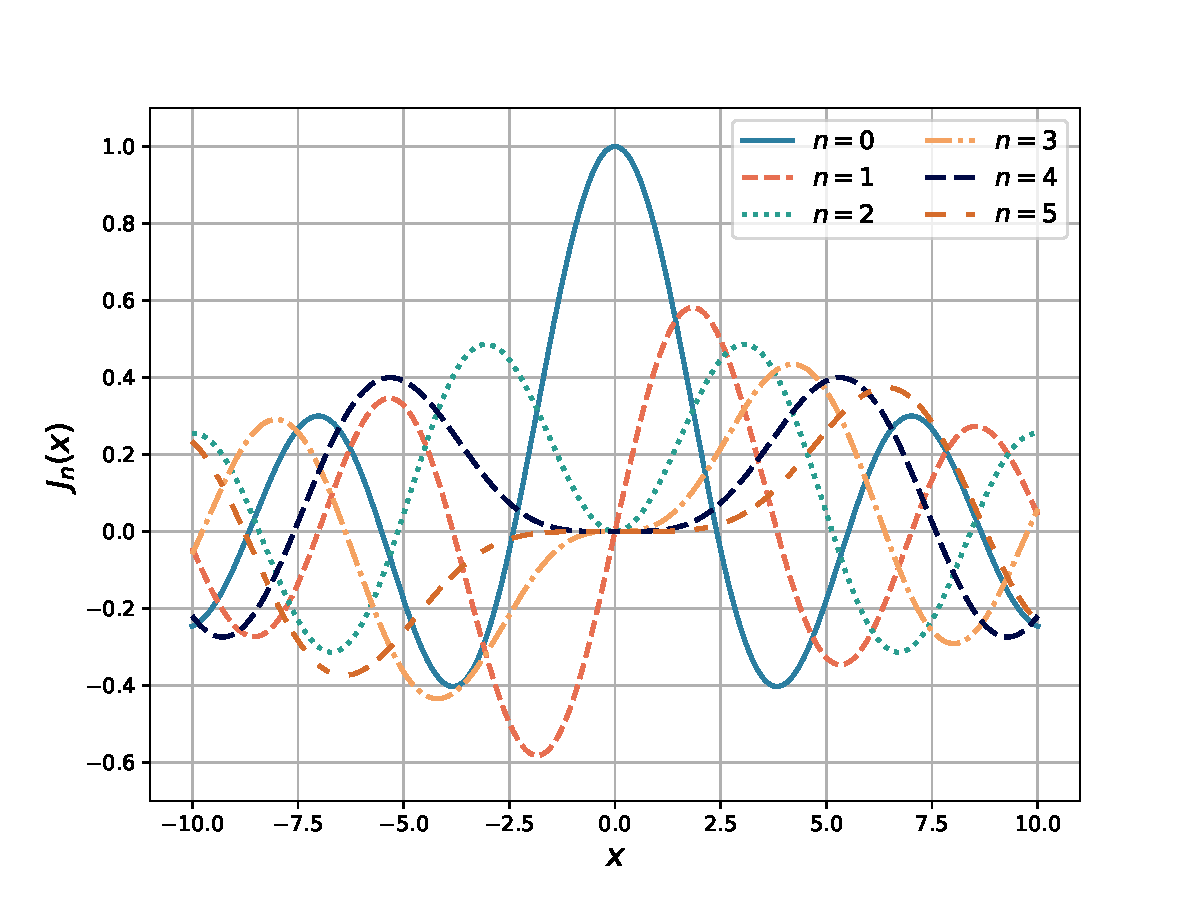
\includegraphics[width = 12cm]{Figuras/Bessel_first_Kind.pdf}
    \caption{Funciones de Bessel de orden entero para $n$ entre 0 y 5. Adaptación de \href{https://github.com/gfrubi/FM2/blob/master/figuras-editables/fig-Bessel.py}{este} código. La adaptación se encuentra \href{aa}{aquí}.}
    % \end{subfigure}
    %
    % \begin{subfigure}[b]{\textwidth}
    %     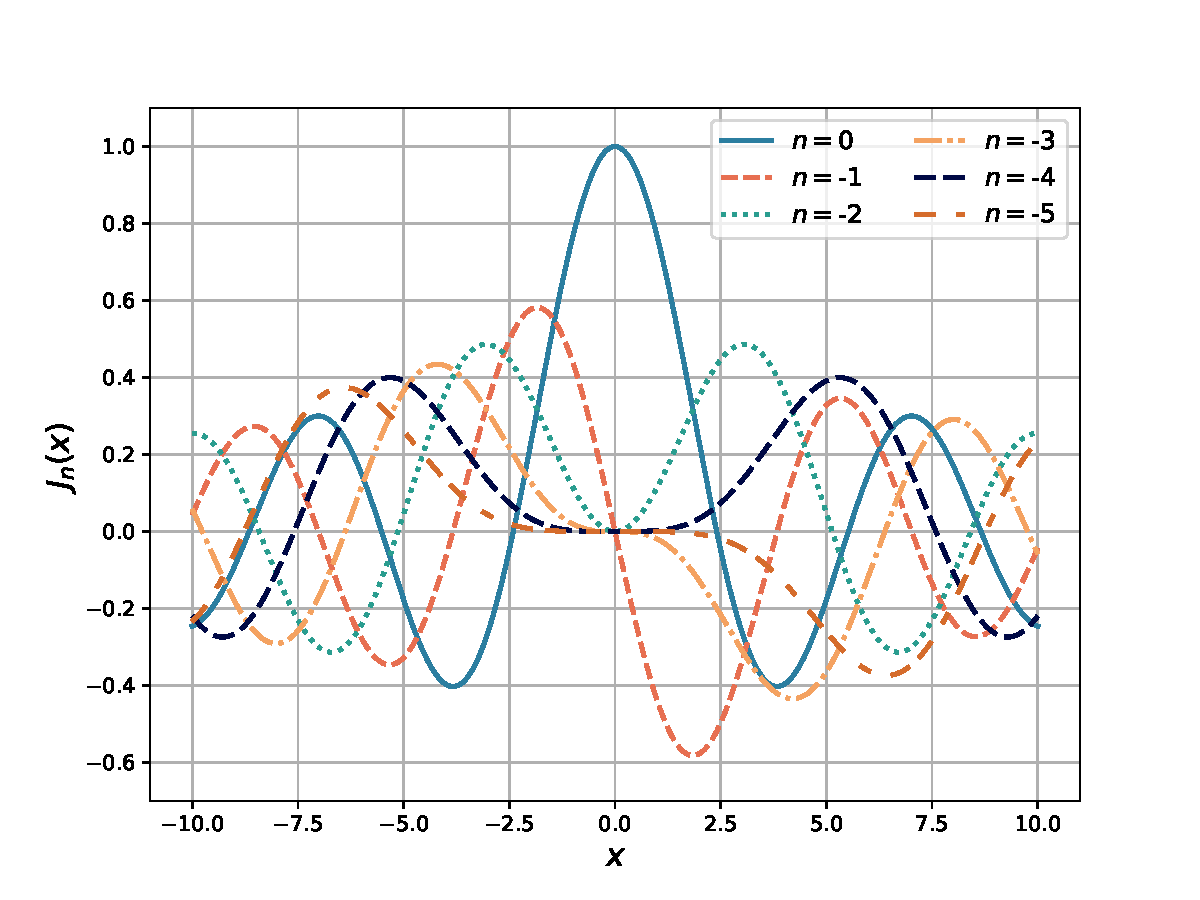
\includegraphics[width = 12cm]{Figuras/Bessel_first_Kind_negative.pdf}
    %     \caption{}
    % \end{subfigure}
    % \caption{aaa}
    \label{fig:Bessel_entero}
\end{figure}

\subsection{Funciones de Bessel de segunda especie, o de Neumann}

Mediante el método de Frobenius, podemos también encontrar soluciones logarítmicas. Mediante este método, podemos encontrar que una segunda solución de este tipo.

\begin{defi} \marginnote{Funciones de Bessel de segunda especie}
    Se denominan \textbf{funciones de Bessel de segunda especie} $Y_\nu(x)$, o \textbf{funciones de Neumann} $N_\nu(x)$ a las soluciones de tipo logarítmica obtenidas a partir del método de Frobenius para la EDO de Bessel \eqref{eq:EDO_Bessel}, linealmente independientes a $J_\nu(x)$.

    Alternativamente, las definimos más comúnmente como
    \begin{equation}
        Y_\nu(x) = N_\nu(x) = \frac{\cos(\pi \nu) J_\nu(x) - J_{-\nu(x)}}{\sin(\pi \nu)} \ , \qquad \nu \notin \mathbb{Z} \ .
    \end{equation}
\end{defi}
% denominada históricamente \textbf{funciones de Neumann} $N_\nu(x)$, o más recientemente \textbf{funciones de Bessel de segunda especie}, $Y_\nu(x)$, como
% \begin{equation}
%     Y_\nu(x) = N_\nu(x) = \frac{\cos(\pi \nu) J_\nu(x) - J_{-\nu(x)}}{\sin(\pi \nu)} \ , \qquad \nu \notin \mathbb{Z} \ ,
% \end{equation}
% que es linealmente independiente a $J_\nu(x)$.\footnote{No se aprecia directamente, pero las funciones de Bessel de segunda especie son soluciones de tipo logarítmicas. Aquí se prefiere utilizar la notación que involucra senos y cosenos por simplicidad, evitando escribir una solución en serie en cada momento.} 

En base a esta definición, podemos también escribir las soluciones generales de la ecuación de Bessel como
\begin{equation}
    y(x) = C_3 J_\nu(x) + C_4 Y_\nu(x) \ .
\end{equation}

La definición dada más arriba es válida para números \emph{no enteros}. Cuando deseamos trabajar con números enteros, es posible demostrar, usando la regla de L'Hôpital, que esta solución sigue siendo linealmente independiente en el límite en que $\nu \to n$, de modo que
\begin{equation}
    Y_n(x) = \lim_{\nu \to n} \frac{\cos(\pi \nu) J_\nu(x) - J_{-\nu(x)}}{\sin(\pi \nu)} \ , \qquad n \in \mathbb{Z} \ .
\end{equation}
Nótese que estas funciones divergen para $x = 0$, como se observa más claramente en la figura \ref{fig:Bessel_segunda_especie}.

De forma similar a las funciones de Bessel de primera especie, estas satisfacen, para orden entero, 
\begin{equation}
    Y_{-n}(x) = (-1)^n Y_n(x) \ .
\end{equation}

\begin{figure}
    \centering
    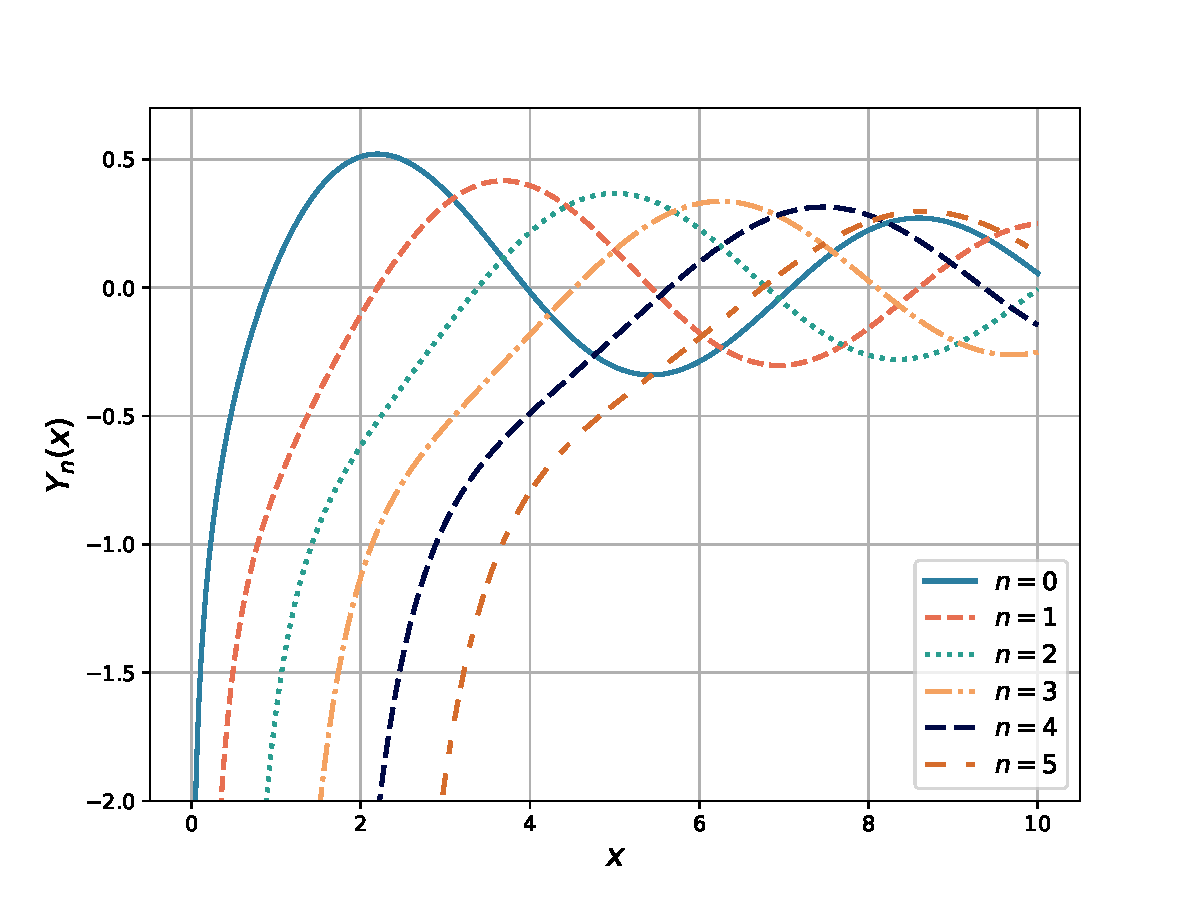
\includegraphics[width = 12cm]{Figuras/Bessel_second_kind.pdf}
    \caption{Funciones de Neumann de orden entero para $n$ entre 0 y 5. Adaptación de \href{https://github.com/gfrubi/FM2/blob/master/figuras-editables/fig-Bessel.py}{este} código. La adaptación se encuentra \href{aa}{aquí}.}
    \label{fig:Bessel_segunda_especie}
\end{figure}

\newpage

\subsection{Funciones de Hankel}

\begin{defi} \marginnote{Funciones de Hankel}
    Se definen las \textbf{funciones de Hankel} $H_\nu^{(1)}(x)$ y $H_\nu^{(2)}(x)$ como dos soluciones linealmente independientes para la EDO de Bessel \eqref{eq:EDO_Bessel}, dadas por
    \begin{align}
        H_\nu^{(1)}(x) & = J_\nu(x) + i Y_\nu(x) \ , \\
        H_\nu^{(2)}(x) & = J_\nu(x) - i Y_\nu(x) \ .
    \end{align}
\end{defi}

¿Por qué definimos otro tipo de soluciones a la EDO de Bessel? Pues es útil trabajar con funciones de Hankel al estudiar soluciones de la ecuación de onda, e históricamente ha sido la ruta a seguir. Además, mediante su representación integral (que mencionaremos más adelante), es posible mostrar\footnote{Puede encontrar el detalle en \cite{Arfken}, pues no considero relevante hacerlo aquí.} que las funciones de Hankel satisfacen las relaciones
\begin{align}
    H_\nu^{(1)}(x) & = e^{-i\nu\pi} H_{-\nu}^{(1)}(x) \ , \\
    H_\nu^{(2)}(x) & = e^{i\nu\pi} H_{-\nu}^{(2)}(x) \ .
\end{align}

% También es útil definir, particularmente al estudiar soluciones de la ecuación de onda, un nuevo conjunto de funciones linealmente independientes, las llamadas \textbf{funciones de Hankel}, que son combinaciones lineales de las funciones de Bessel y Neumann,
% \begin{align}
%     H_\nu^{(1)}(x) & = J_\nu(x) + Y_\nu(x) \ , \\
%     H_\nu^{(2)}(x) & = J_\nu(x) - Y_\nu(x) \ .
% \end{align}

% Mediante su representación integral (que mencionaremos más adelante), es posible mostrar\footnote{En este caso, el detalle puede encontrarse en \cite{Arfken}.} que las funciones de Hankel satisfacen las relaciones
% \begin{align}
%     H_\nu^{(1)}(x) = e^{-i\nu\pi} H_{-\nu}^{(1)}(x) \ , \\
%     H_\nu^{(2)}(x) = e^{i\nu\pi} H_{-\nu}^{(2)}(x) \ .
% \end{align}


\subsection{Función generatriz (para orden entero)}

En el caso en que $\nu$ es un número entero, podemos escribir una función generatriz de una forma análoga a cualquier polinomio ortogonal, a pesar de que las funciones de Bessel no son polinomios. En este caso, esta tiene la forma
\begin{equation}
    G(x,t) = \exp\left[ \frac{x}{2} \left( t - \frac{1}{t} \right) \right] = \sum_{n = -\infty}^\infty J_n(x) t^n \ .
\end{equation}
Es directo verificar la segunda igualdad al expandir la exponencial en una serie de potencias para $t$. Gracias a la función generatriz, podemos hallar de una forma más sencilla algunas propiedades para las funciones de Bessel de orden entero.

\subsection{Ceros de las funciones de Bessel}

Las funciones de Bessel son funciones oscilantes, pero no periódicas. Por ello, si bien tienen infinitos ceros (puntos para los cuales $J_\nu(x) = 0$), no existe una forma analítica de calcularlos. Por este motivo, estos valores son calculados de forma numérica a partir de, por ejemplo, la expresión en serie para las funciones de Bessel. Denotaremos la $n-$ésima raíz de la función de Bessel de orden $\nu$ como $\alpha_{\nu, n}$, tal que $J(\alpha_{\nu, n}) = 0$. Además, estas cumplen que $\alpha_{\nu, n+1} > \alpha_{\nu, n}$. Mostramos algunos ceros para funciones de orden entero en la tabla \ref{tab:alphanun}.

\begin{table}[htbp]
    \centering
    \begin{tabular}{ccccccc}
    \hline $\alpha_{\nu,n}$ & $n=1$ & $n=2$ & $n=3$ & $n=4$ & $n=5$ \\ \hline 
    $\nu=0$ & 2.4048255 &  5.5200781 &  8.6537279 & 11.7915344 & 14.9309177\\
    $\nu=1$ & 3.8317059 &  7.0155866 & 10.1734681 & 13.3236919 & 16.4706300\\
    $\nu=2$ & 5.1356223 &  8.4172441 & 11.6198411 & 14.7959517 & 17.9598194 \\
    $\nu=3$ & 6.3801619 &  9.7610231 & 13.0152007 & 16.2234661 & 19.4094152 \\
    $\nu=4$ & 7.5883424 & 11.0647094 & 14.3725366 & 17.6159660 & 20.8269329 \\
    \hline 
    \end{tabular} 
    \caption{Las primeras raíces $\alpha_{\nu,n}$ de $J_\nu(x)$, $\nu=0,1,2,3,4$. Un Código Python para hallarlas se encuentra disponible en \href{https://github.com/gfrubi/FM2/blob/master/Notebooks/Bessel-Ceros.ipynb}{este} notebook.}
    \label{tab:alphanun}
\end{table}

De igual manera, a veces es necesario utilizar los ceros de las derivadas de las funciones de Bessel, los que denotaremos por $\beta_{\nu, n}$. Ellos, al igual que los $\alpha_{\nu, n}$, satisfacen que $\beta_{\nu, n+1} > \beta_{\nu, n}$. Algunos valores numéricos se presentan en la tabla \ref{tab:betanun}.

\begin{table}[htbp]
    \centering
    \begin{tabular}{ccccccc}
    \hline $\beta_{m,n}$ & $n=1$ & $n=2$ & $n=3$ & $n=4$ & $n=5$ \\ \hline 
    $m=0$ & 3.8317059 &  7.0155866 & 10.1734681 & 13.3236919 & 16.4706300\\
    $m=1$ & 1.8411837 &  5.3314427 &  8.5363163 & 11.7060049 & 14.8635886 \\
    $m=2$ & 3.0542369 &  6.7061331 &  9.9694678 & 13.1703708 & 16.3475223 \\
    $m=3$ & 4.2011889 &  8.0152366 & 11.3459243 & 14.5858482 & 17.7887478 \\
    $m=4$ & 5.3175531 &  9.2823962 & 12.6819084 & 15.9641070 & 19.1960288 \\
    \hline 
    \end{tabular} 
    \caption{Las primeras raíces $\beta_{m,n}$ de $J'_m(x)$, $m=0,1,2,3,4$. Un Código Python para hallarlas se encuentra disponible en \href{https://github.com/gfrubi/FM2/blob/master/Notebooks/Bessel-Ceros.ipynb}{este} notebook.}
    \label{tab:betanun}
\end{table}


\subsection{Propiedades}
\begin{propiedad}
    \textbf{Propiedades de las funciones de Bessel}

    \begin{enumerate}
        % \item \textbf{Normalización.} Dada una raíz $\alpha_{\nu, n}$ de la función de Bessel de orden $\nu$, se satisface que
        % \begin{equation}
        %     \int_0^a r \left[J_\nu\left( \alpha_{\nu, n} \frac{x}{a} \right)\right]^2 dr = \frac{a^2}{2} \left[ J_{\nu+1}(\alpha_{\nu, n}) \right]^2 \ . 
        % \end{equation}
        \item \textbf{Ortogonalidad respecto a las raíces.} Para valores de $\nu$ no negativos, para $a > 0$ y para $n, m \in \mathbb{N}$, se tiene que
        \begin{equation}
            \int_0^a x J_{\nu} \left( \frac{\alpha_{\nu, n}}{a} x \right) J_\nu\left( \frac{\alpha_{\nu, m}}{a} x \right) dx = \frac{a^2}{2} [J'_\nu(\alpha_{\nu, n})]^2 \delta_{n, m} = \frac{a^2}{2} [J_{\nu+1}(\alpha_{\nu, n})]^2 \delta_{n, m} \ .
        \end{equation}
        Similarmente, para las raíces de la derivada de la función de Bessel, se tiene
        \begin{equation}
            \int_0^a x J_\nu\left(\frac{\beta_{\nu, n}}{a}x \right) J_\nu\left(\frac{\beta_{\nu, m}}{a}x \right) dx = \frac{a^2}{2} \left( 1 - \frac{\nu^2}{\beta^2_{\nu, n}} \right) \left[ J_\nu(\beta_{\nu, n}) \right]^2 \ .
        \end{equation}
        % 
        % En general, dadas dos constantes $u, v$, y dado el intervalo $[a,b]$, las funciones de Bessel satisfacen
        % \begin{equation}
        %     \int_a^b x J_\nu(u x) J_\nu(bx) dx = \frac{1}{u^2-v^2} \left[ vx J_\nu(ux) J0_\nu(vx) - ux J_\nu(vx) J'_\nu(ux) \right]_a^b \delta_{u,v} \ .
        % \end{equation} 
        \item \textbf{Ortogonalidad respecto al orden.} Las funciones de Bessel, en general, \emph{no son ortogonales respecto a los índices}, es decir, $\left\langle J_\mu(x), J_\nu(x) \right\rangle \neq 0$.
        \item \textbf{Completitud.} Las funciones de Bessel (de orden no negativo) forman un \emph{conjunto completo} de funciones en el intervalo $[0,a]$, lo que se puede representar aproximadamente como \cite{Reimberg2015}
        \begin{equation}
            \sum_{k=1}^\infty \frac{J_{\nu-1} \left(\frac{ \alpha_{\mu, k}}{a}x \right) J_{\nu-1} \left(\frac{\alpha_{\mu, k}}{a} y \right)}{\left[J_{\mu+1}(\alpha_{\mu, k})\right]^2} = \frac{a}{2x} \delta\left( \frac{x}{a} - \frac{y}{a} \right) \ ,
        \end{equation}
        donde $\mu + 1 \geq \nu$, y $\mu - \nu > 1$.
        % \begin{equation}
        %     \int_0^\infty x J_\nu(ux) J_\nu(vx) dx = \frac{1}{u} \delta(u-v) \ ,
        % \end{equation}
        % para cualquier $\nu > -1/2$.
        \item \textbf{Serie de Fourier-Bessel.} Dado que las funciones de Bessel forman una base en el intervalo $[0,a]$, podemos expandir cualquier función en una Serie de Fourier-Bessel, tal que
        \begin{equation}
            f(x) = \sum_{n=0}^\infty c_{\nu, n} \ J_\nu\left(\alpha_{\nu, n} \frac{x}{a}\right) \ ,
        \end{equation}
        donde
        \begin{equation}
            c_{\nu, n} = \frac{2}{a^2 \left[J_{\nu+1}(\alpha_{\nu, n})\right]^2} \int_0^a x f(x) \ J_\nu\left( \alpha_{\nu, k} \frac{x}{a} \right) dx \ .
        \end{equation}
        \item \textbf{Representación Integral.} Por motivos históricos, las funciones de Bessel fueron encontradas como soluciones a ecuaciones integrales. Por ello, listamos las representaciones integrales más comunes, que pueden ser obtenidas como una Serie de Laurent de la función generatriz.
        \begin{align}
            J_n(x) & = \frac{1}{\pi}\int_0^\pi \cos(nt - x\sin t) dt \ , \\
            J_\nu(x) & = \frac{1}{\pi} \int_0^\pi \cos(\nu t - x\sin t) dt - \frac{\sin(\nu \pi)}{\pi} \int_0^\infty e^{-x \sinh t - \nu t} dt \ , \\
            Y_n(x) & = \frac{1}{\pi} \int_0^\pi \sin(x\sin t - nt) dt - \frac{1}{\pi} \int_0^\infty \left[e^{nt} + (-1)^n e^{-nt} \right] e^{-x \sinh t} dt \ .
        \end{align}
    
        Gracias a ellas, podemos obtener tres resultados interesantes, los que son 
        \begin{align}
            \cos(x \sin \theta) & = J_0(x) + 2 \sum_{n*1}^\infty J_{2n}(x) \cos(2n\theta) \ , \\
            \sin(x \sin \theta) & = 2 \sum_{n=1}^\infty J_{2n-1}(x) \sin((2n-1)\theta) \ ,
        \end{align}
        y para el caso en que $\theta = 0$, 
        \begin{equation}
            J_0(x) + 2\sum_{n=1}^\infty J_{2n}(x) = 1 \ .
        \end{equation}
        \item \textbf{Comportamiento asintótico.} En el límite en que $x$ toma valores \emph{muy grandes}, generalmente entendido como $x \gg |\nu^2 - 1/4|$, podemos representar las funciones de Bessel como
        \begin{align}
            J_\nu(x) & \approx \sqrt{\frac{2}{\pi x}} \cos\left( x - \frac{\nu \pi}{2} - \frac{\pi}{4} \right) \ , \\
            Y_\nu(x) & \approx \sqrt{\frac{2}{\pi x}} \sin\left( x - \frac{\nu \pi}{2} - \frac{\pi}{4} \right) \ , \\
            H^{(1)}_\nu(x) = H^{(2)}_\nu(x)^\ast & = \sqrt{\frac{2}{\pi x}} \exp\left[ i \left( x - \frac{\nu \pi}{2} - \frac{\pi}{4} \right) \right] \ .
        \end{align}
        \item \textbf{Relaciones de Recurrencia.} Por definición, cualquier función de Bessel (incluyendo las de Neumann y de Hankel) debe satisfacer las siguientes relaciones de recurrencia:
        \begin{align}
            Z_{n+1}(x) + Z_{n-1}(x) & = \frac{2n}{x} Z_n(x) \ , \\
            Z_{n+1}(x) - Z_{n-1}(x) & = -2 Z'_n(x) \ . 
        \end{align}

        \item \textbf{Relaciones con derivadas.} A partir de las relaciones de recurrencia, es posible mostrar que cualquier función de Bessel satisface
        \begin{align}
            x^\nu Z_{\nu-1}(x) & = \frac{d}{dx}\left[ x^\nu Z_\nu(x) \right] \ , \\
            -x^{-\nu} Z_{\nu+1}(x) & = \frac{d}{dx}\left[ x^{-\nu} Z_\nu(x) \right] \ , \\
            \frac{d}{dx} \left[ Z_\nu(x) \right] & = \frac{1}{2} \left[ Z_{\nu-1}(x) - Z_{\nu+1}(x) \right] \ .
        \end{align}
    \end{enumerate}
\end{propiedad}


\section{Funciones modificadas de Bessel}

¿Qué pasaría si, en la ecuación \eqref{eq:EDO_Bessel}, $x^2$ tuviera signo negativo en lugar de positivo? Es decir, si la ecuación toma la forma
\begin{equation}\label{eq:Bessel_modificada}
    x^2 \frac{d^2y}{dx^2} + x \frac{dy}{dx} - (x^2 + \nu^2)y = 0 \ . 
\end{equation}

Esta ecuación es conocida como la \textbf{ecuación modificada de Bessel}, y sus soluciones, a diferencia de las funciones de Bessel, \emph{no son oscilantes}, sino que su comportamiento es exponencial. Por suerte, métodos análogos a los utilizados anteriormente nos permiten encontrar soluciones a esta ecuación.

\begin{defi} \marginnote{Funciones modificadas de Bessel}
    Un conjunto particular de soluciones a la ecuación modificada de Bessel \eqref{eq:Bessel_modificada} corresponde a las \textbf{funciones modificadas de Bessel de primera especie}, $I_\nu(x)$, y a las \textbf{funciones modificadas de Bessel de segunda especie}, $K_\nu(x)$, definidas como
    \begin{align}
        I_\nu(x) & = i^{-\nu} J_\nu(ix) = \sum_{k=0^\infty} \frac{1}{k! \Gamma(k+\nu+1)} \left( \frac{x}{2} \right)^{2k+\nu} \ , \\
        K_\nu(x) & = i^{\nu + 1} \frac{\pi}{2} H_\nu^{(1)}(ix) = \frac{\pi}{2} \left[ \frac{I_{-\nu}(x) - I_\nu(x)}{\sin(\nu \pi)} \right] \ , \qquad \nu \notin \mathbb{Z} \ .
    \end{align}
\end{defi}

De forma análoga a lo ocurrido para las funciones de Bessel de segunda especie, en caso en que $\nu$ sea entero, las funciones modificadas de segunda especie se definen como el límite
\begin{equation}
    K_n(x) = \lim_{\nu \to n} \frac{\pi}{2} \left[ \frac{I_{-\nu}(x) - I_\nu(x)}{\sin(\nu \pi)} \right] \ , \qquad n \in \mathbb{Z} \ .
\end{equation}

\begin{figure}[htbp]
    \centering
    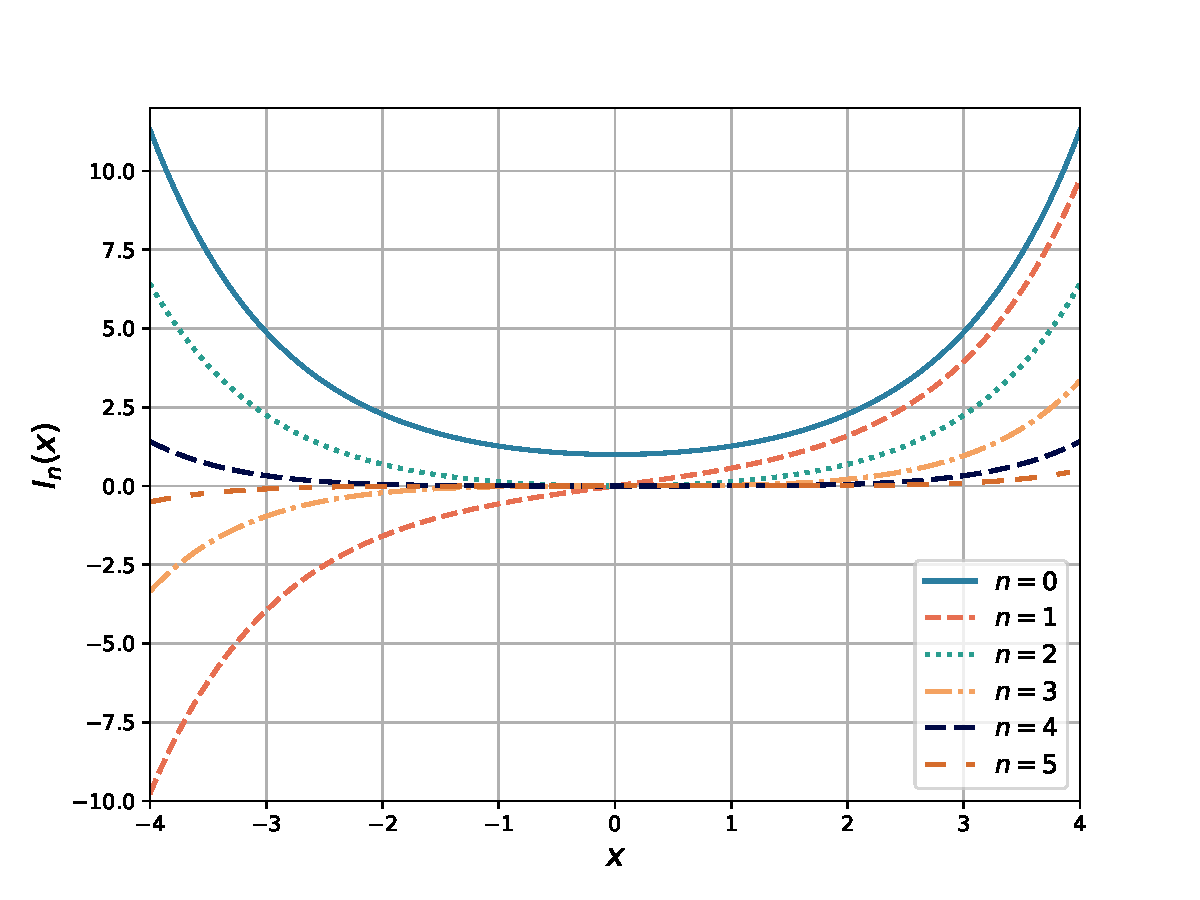
\includegraphics[width = 10cm]{Figuras/Bessel-modified-first-kind.pdf}
    \caption{Funciones de Bessel modificadas de primera especie. Figura adaptada a partir de \href{https://github.com/gfrubi/FM2/blob/master/figuras-editables/fig-Bessel.py}{este} código. La adaptación se encuentra \href{aa}{aquí}.}
    \label{fig:Bessel_modificada_primera}
\end{figure}

\begin{figure}[htbp]
    \centering
    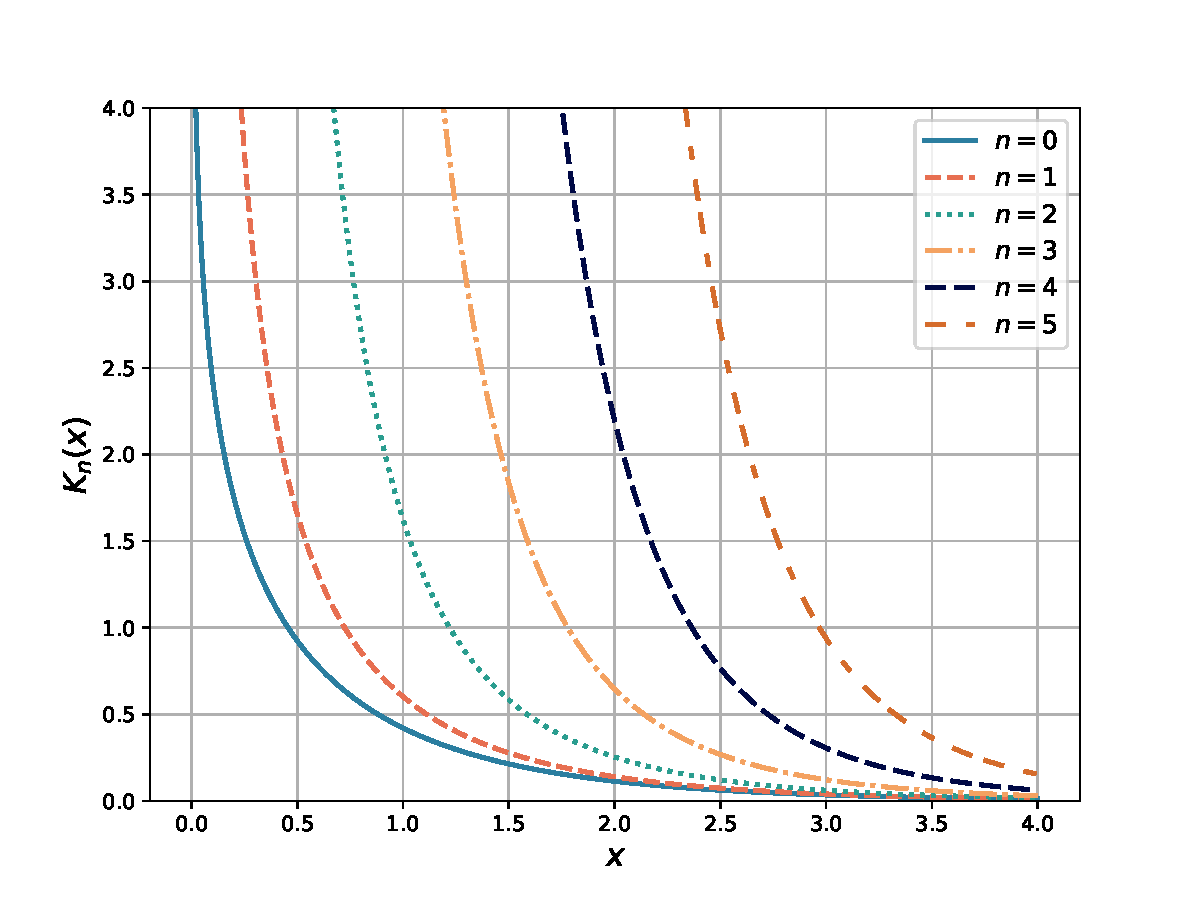
\includegraphics[width = 10cm]{Figuras/Bessel-modified-second-kind.pdf}
    \caption{Funciones de Bessel modificadas de segunda especie. Figura adaptada a partir de \href{https://github.com/gfrubi/FM2/blob/master/figuras-editables/fig-Bessel.py}{este} código. La adaptación se encuentra \href{aa}{aquí}.}
    \label{fig:Bessel_modificada_segunda}
\end{figure}

% \begin{figure}[htbp]
%     \centering
%     \begin{subfigure}{\textwidth}
%         \centering
%         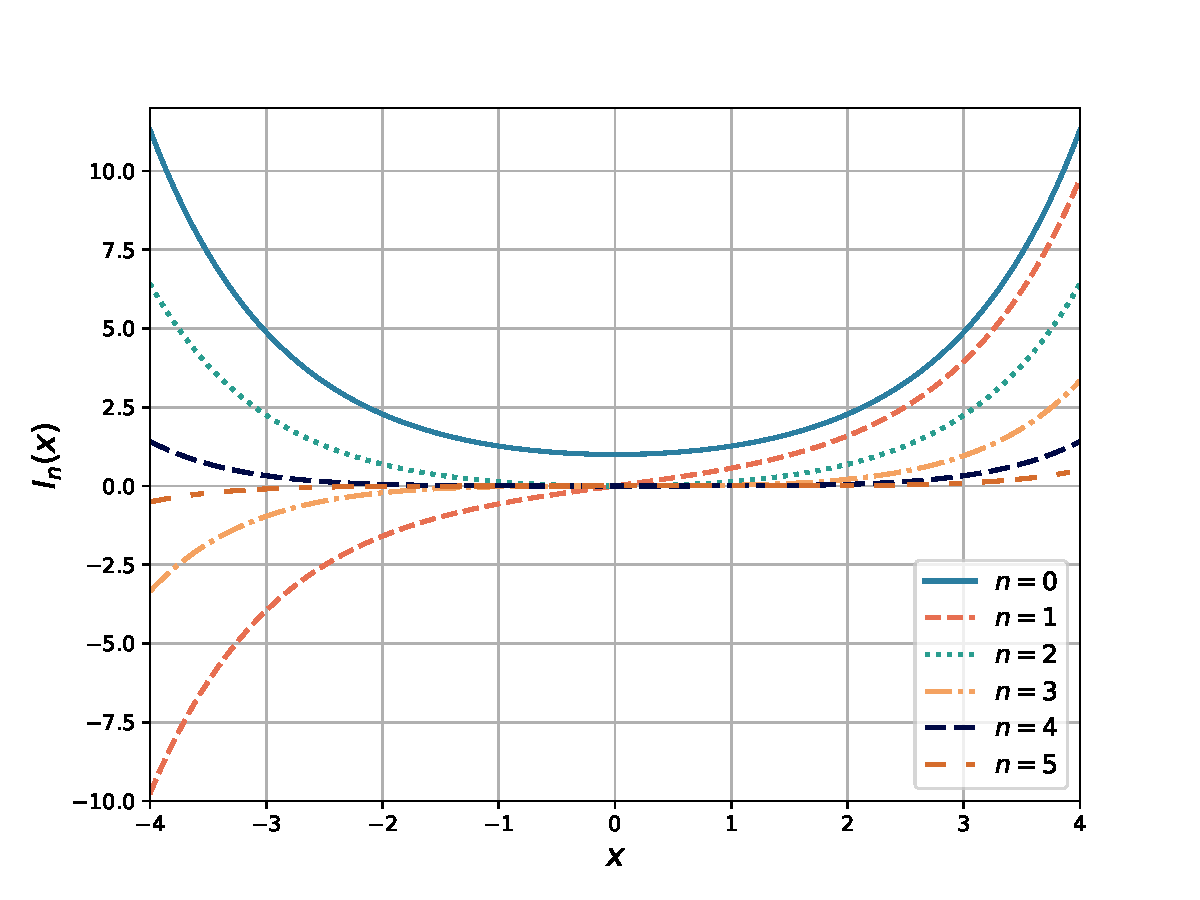
\includegraphics[width = 10cm]{Figuras/Bessel-modified-first-kind.pdf}
%         \caption{\label{fig:Bessel_modificada_primera}}
%     \end{subfigure}
%     \begin{subfigure}{\textwidth}
%         \centering
%         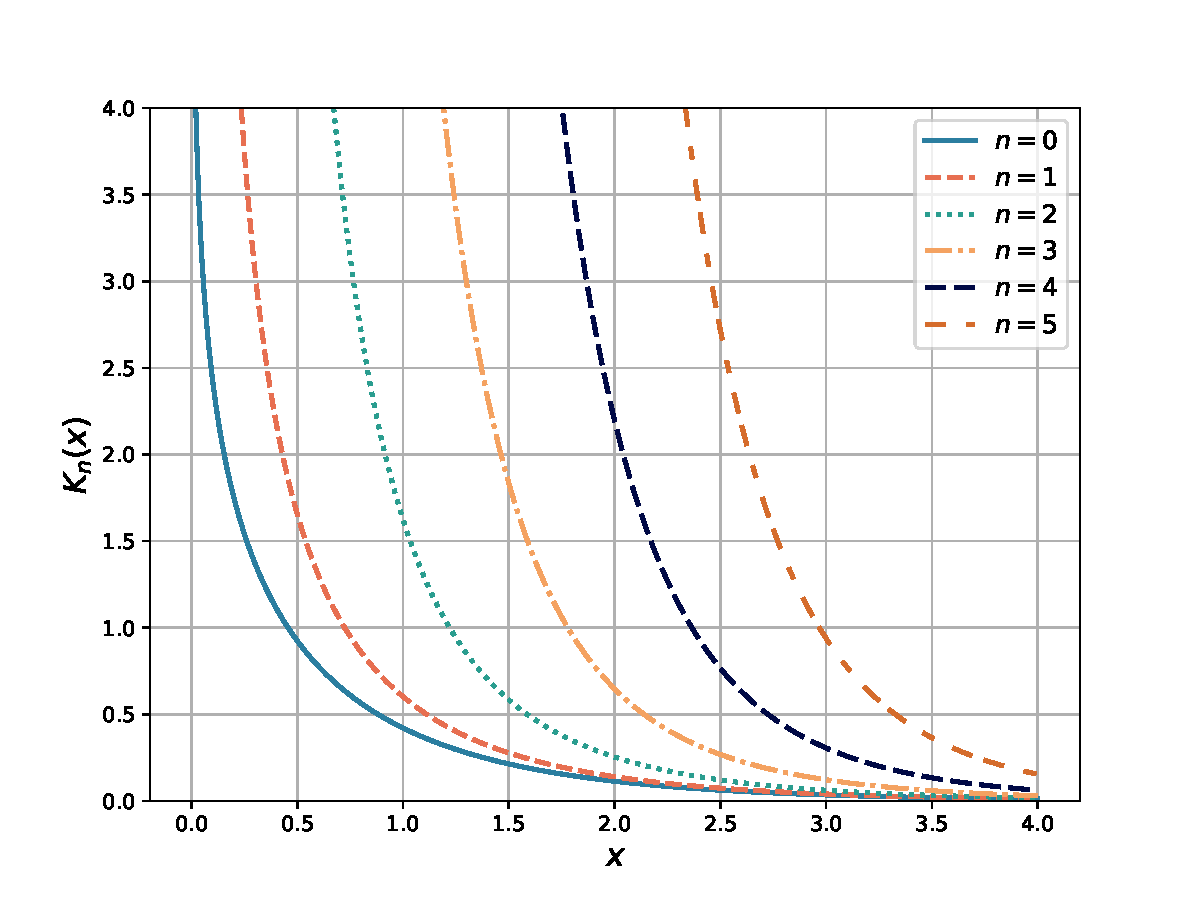
\includegraphics[width = 10cm]{Figuras/Bessel-modified-second-kind.pdf}
%         \caption{\label{fig:Bessel_modificada_segunda}}
%     \end{subfigure}
%     \caption{Funciones de Bessel modificadas de \subref{fig:Bessel_modificada_primera} primera especie y \subref{fig:Bessel_modificada_segunda} segunda especie. Figura adaptada a partir de \href{https://github.com/gfrubi/FM2/blob/master/figuras-editables/fig-Bessel.py}{este} código. La adaptación se encuentra \href{aa}{aquí}.}
%     \label{fig:Bessel_modificada}
% \end{figure}

\subsection{Propiedades}

\begin{propiedad}
    \textbf{Propiedades de las funciones modificadas de Bessel.}

    \begin{enumerate}
        \item \textbf{Comportamiento asintótico.} En el límite en que $x$ toma valores \emph{muy grandes}, generalmente entendido como $x \gg |\nu^2 - 1/4|$, podemos representar las funciones de Bessel como
        \begin{align}
            I_\nu(x) & = \frac{1}{\sqrt{2\pi x}} e^x \ , \\
            K_\nu(x) & = \sqrt{\frac{\pi}{2x}} e^{-x} \ . 
        \end{align}
        \item \textbf{Relaciones de recurrencia.} Las funciones modificadas de Bessel satisfacen las siguientes relaciones de recurrencia,
        \begin{align}
            I_{\nu - 1}(x) - I_{\nu + 1}(x) & =   \frac{2\nu}{x} I_\nu(x) \ , \\
            K_{\nu - 1}(x) - K_{\nu + 1}(x) & = - \frac{2\nu}{x} K_\nu(x) \ , \\
            I_{\nu - 1}(x) + I_{\nu + 1}(x) & =   2 I'_\nu(x) \ , \\
            K_{\nu - 1}(x) + K_{\nu + 1}(x) & = - 2 K'_\nu(x) \ .
        \end{align}
        \item \textbf{Relaciones con derivadas.} A partir de las relaciones de recurrencia, podemos hallar las relaciones
        \begin{align}
            x^{\nu} I_{\nu - 1}(x)    & = \frac{d}{dx}[x^\nu    I_\nu(x)] \ , \\
            - x^{\nu} K_{\nu - 1}(x)  & = \frac{d}{dx}[x^\nu    K_\nu(x)] \ , \\
            x^{-\nu} I_{\nu + 1}(x)   & = \frac{d}{dx}[x^{-\nu} I_\nu(x)] \ , \\
            - x^{-\nu} K_{\nu + 1}(x) & = \frac{d}{dx}[x^{-\nu} K_\nu(x)] \ .
        \end{align}
    \end{enumerate}
\end{propiedad}

\begin{ejemplo}
    \textbf{(Butkov, sección 9.11.)} Considere un cilindro circular sólido de radio $b$ y longitud $L$. Las bases del cilindro se mantienen a temperatura cero, $u(z = 0, t) = u(z = L, t) = 0$, mientras que su superficie lateral es mantenida a una temperatura $u(\rho = b, t) = T_1$ constante. Encuentre la distribución de temperatura en el interior del cilindro en el estado estacionario.

    \textbf{Solución.} Cuando nos referimos a \emph{estado estacionario}, nos referimos al caso en que la temperatura se mantenga constante en el tiempo. Dado este requisito, la ecuación de difusión del calor se convertirá en la ecuación de Laplace, pues
    \begin{equation*}
        \nabla^2 u = \frac{1}{\alpha^2} \cancelto{0}{\frac{\partial u}{\partial t}} = 0 \ .
    \end{equation*}
    Dado que el sistema es un cilindro, también imponemos la condición de periodicidad sobre la variable angular, es decir, $u(\rho, \phi, z) = u(\rho, \phi + 2\pi, z)$. Realizando separación de variables, tendremos las ecuaciones
    \begin{align*}
        \frac{d^2 Z}{dz^2} & = \lambda_1 Z \ , \\
        \frac{d^2 \Phi}{d\phi^2} & = \lambda_2 \Phi \ , \\
        \frac{d}{d\rho}\left( \rho \frac{dP}{d\rho} \right) + \left[ \rho \lambda_1 + \frac{\lambda_2}{\rho} \right] & = 0 \ .
    \end{align*} 
    Imponiendo nuestras condiciones de contorno, concluimos que $\lambda_1 = -n^2 \pi^2/L^2$ para $n = 1, 2, 3, \dots$ (solución oscilante), y $\lambda_2 = -m^2$ para $m = 0, 1, 2, \dots$ Así, la ecuación para $P$ se convierte en
    \begin{equation*}
        \frac{d}{d\rho}\left( \rho \frac{dP}{d\rho} \right) - \left[ \rho \frac{n^2\pi^2}{L^2} + \frac{m^2}{\rho} \right] = 0 \ ,
    \end{equation*} 
    lo que corresponde a la EDO modificada de Bessel. Esto se aprecia de forma más clara bajo el cambio de variable $x = n\pi \rho/L$, $P(\rho) = y(x)$, donde tendremos
    \begin{equation*}
        x^2 \frac{d^2 y}{dy^2} + x \frac{dy}{dx} - (x^2 + m^2)y = 0 \ .
    \end{equation*}

    Esta EDO tiene por solución general a las funciones modificadas de Bessel, tal que
    \begin{equation*}
        P_{mn}(\rho) = A_{mn} I_m\left( \frac{n\pi \rho}{L} \right) + B_{mn} K_m\left( \frac{n\pi \rho}{L} \right) \ .
    \end{equation*}

    Ahora, dado que trabajamos con un cilindro de radio finito, $\rho \to \infty$ no es parte de nuestro dominio, por lo que la función $I_m(x)$ está definida para nuestro problema. En cambio, dado que $\rho = 0$ es parte de nuestro dominio, y la función $K_m(x)$ diverge para $x = 0$, descartamos esta solución imponiendo que $B_{mn} = 0$.

    Por otro lado, dado que nuestro sistema posee simetría axial como consecuencia de la condición de contorno $u(\rho = b) = T_1$, pues este valor es válido para cualquier valor de $\phi$, podemos concluir que basta con considerar el caso en que $m=0$, de modo que la solución para $P(\rho)$ es dada por
    \begin{equation*}
        P_n(\rho) = A_n I_0\left( \frac{n \pi \rho}{L} \right) \ ,
    \end{equation*}
    mientras que la solución general al problema es de la forma
    \begin{equation*}
        u(\rho, \phi, z) = \sum_{n=1}^\infty A_n \sin\left( \frac{n \pi z}{L} \right) I_0 \left( \frac{n \pi \rho}{L} \right) \ ,
    \end{equation*}
    donde el coeficiente $A_n$ se obtiene imponiendo la condición de contorno $u(\rho = b) = T_1$. Queda como ejercicio para el lector comprobar que luego de imponer la condición de contorno, la solución a nuestro problema será
    \begin{equation*}
        u(\rho, \phi, z) = \frac{4T_1}{\pi} \sum_{n=1, 3, 5, \dots}^\infty \frac{1}{n} \frac{I_0(n \pi \rho/L) \sin(n \pi z/L)}{I_0(n \pi b/L)} \ .
    \end{equation*}
\end{ejemplo}

% las que corresponden a las \textbf{funciones modificadas de Bessel de primera especie}, $I_\nu(x)$, y a las \textbf{funciones modificadas de Bessel de segunda especie}, $K_\nu(x)$, definidas como
% \begin{align}
%     I_\nu(x) & = i^{-\nu} J_\nu(ix) = \sum_{k=0^\infty} \frac{1}{k! \Gamma(k+\nu+1)} \left( \frac{x}{2} \right)^{2k+\nu} \ , \\
%     K_\nu(x) & = \frac{\pi}{2} \left[ \frac{I_{-\nu}(x) - I_\nu(x)}{\sin(\nu \pi)} \right] \ , \qquad \nu \notin \mathbb{Z} \ , \\
%     K_n(x) & = \lim_{\nu \to n} \frac{\pi}{2} \left[ \frac{I_{-\nu}(x) - I_\nu(x)}{\sin(\nu \pi)} \right] \ , \qquad n \in \mathbb{Z} \ .
% \end{align}

\section{Funciones esféricas de Bessel}

Hemos discutido que las funciones de Bessel surgen como solución de la \emph{EDO radial} que surge de separar la ecuación de Helmholtz para coordenadas cilíndricas, que denominamos EDO de Bessel. De manera análoga, la EDO radial que surge en coordenadas esféricas es denominada \textbf{ecuación esférica de Bessel}, y es dada por
\begin{equation}
    x^2 \frac{d^2y}{dx^2} + 2x \frac{dy}{dx} + (x^2 - \ell(\ell+1))y = 0 \ ,
\end{equation}
donde hemos realizado el cambio de variables $x = kr$.

% Si bien las incluímos en el mismo capítulo dado su nombre, las \textbf{funciones esféricas de Bessel} surgen como soluciones de la parte radial de la ecuación de Helmholtz \emph{en coordenadas esféricas}, donde en la ecuación X hallamos que la ecuación esférica de Bessel es
% \begin{equation}
%     r^2 \frac{d^2R}{dr^2} + 2r \frac{dR}{dr} + [k^2 r^2 - \ell (\ell+1)]R(r) = 0 \ ,
% \end{equation}
% donde $\ell$ es un número entero. 
Notemos que, bajo la sustitución $y(x) = x^{-1/2} S(x)$, la ecuación toma la forma
\begin{equation} \label{eq:EDO_esferica_Bessel}
    x^2 \frac{d^2 S}{dx^2} + x \frac{dS}{dx} + \left[x^2 - \left(\ell + \frac{1}{2}\right)^2\right]S = 0 \ ,
\end{equation}
que al comparar con \eqref{eq:EDO_Bessel}, notamos que corresponde a la ecuación de Bessel de orden $\ell + 1/2$. Por ello, una solución de esta ecuación será
\begin{equation}
    y(x) = C_1 \frac{J_{\ell + 1/2}(x)}{\sqrt{x}} + C_2 \frac{Y_{\ell + 1/2}(x)}{\sqrt{x}} \ ,
\end{equation}
donde las constantes $C_1$ y $C_2$ se determinan a partir de las condiciones de contorno. En particular, cuando deseamos soluciones que sean finitas en el origen, escogeremos $C_2 = 0$.

\begin{defi} \marginnote{Funciones esféricas de Bessel}
    Las \textbf{funciones esféricas de Bessel} de primera y segunda especie corresponden a las soluciones de la ecuación esférica de Bessel \eqref{eq:EDO_esferica_Bessel} dadas por
    \begin{align}
        j_\ell(x) & = \sqrt{\frac{\pi}{2x}} J_{\ell + 1/2}(x) \ , \\
        y_\ell(x) = n_\ell(x) & = \sqrt{\frac{\pi}{2x}} Y_{\ell + 1/2}(x) \ .
    \end{align}
\end{defi}

% Bajo una normalización adecuada, preferimos definir las \textbf{funciones esféricas de Bessel} de primera y segunda especie como
% \begin{align}
%     j_\ell (x) & = \sqrt{\frac{\pi}{2x}} J_{\ell + 1/2}(x) \ , \\
%     y_\ell (x) = n_\ell(x) & = \sqrt{\frac{\pi}{2x}} Y_{\ell + 1/2} \ ,
% \end{align}
% donde, para $\ell$ entero, $Y_{\ell + 1/2}(x) = (-1)^{\ell + 1}J_{-\ell - 1/2}(x)$. 
Vale la pena hacer notar que
\begin{align}
    j_0(x) & = \frac{\sin x}{x} \ , \\
    y_0(x) & = - \frac{\cos x}{x} \ .
\end{align}
Además, cuando $\ell$ corresponde a un número entero, las funciones esféricas de Bessel satisfacen que
\begin{equation}
    y_{\ell+1/2}(x) = (-1)^{\ell+1} j_{-\ell - 1/2}(x) \ ,
\end{equation}
lo que es consecuencia de su relación con las funciones de Bessel de orden semientero.

\begin{figure}[htbp]
    \centering
    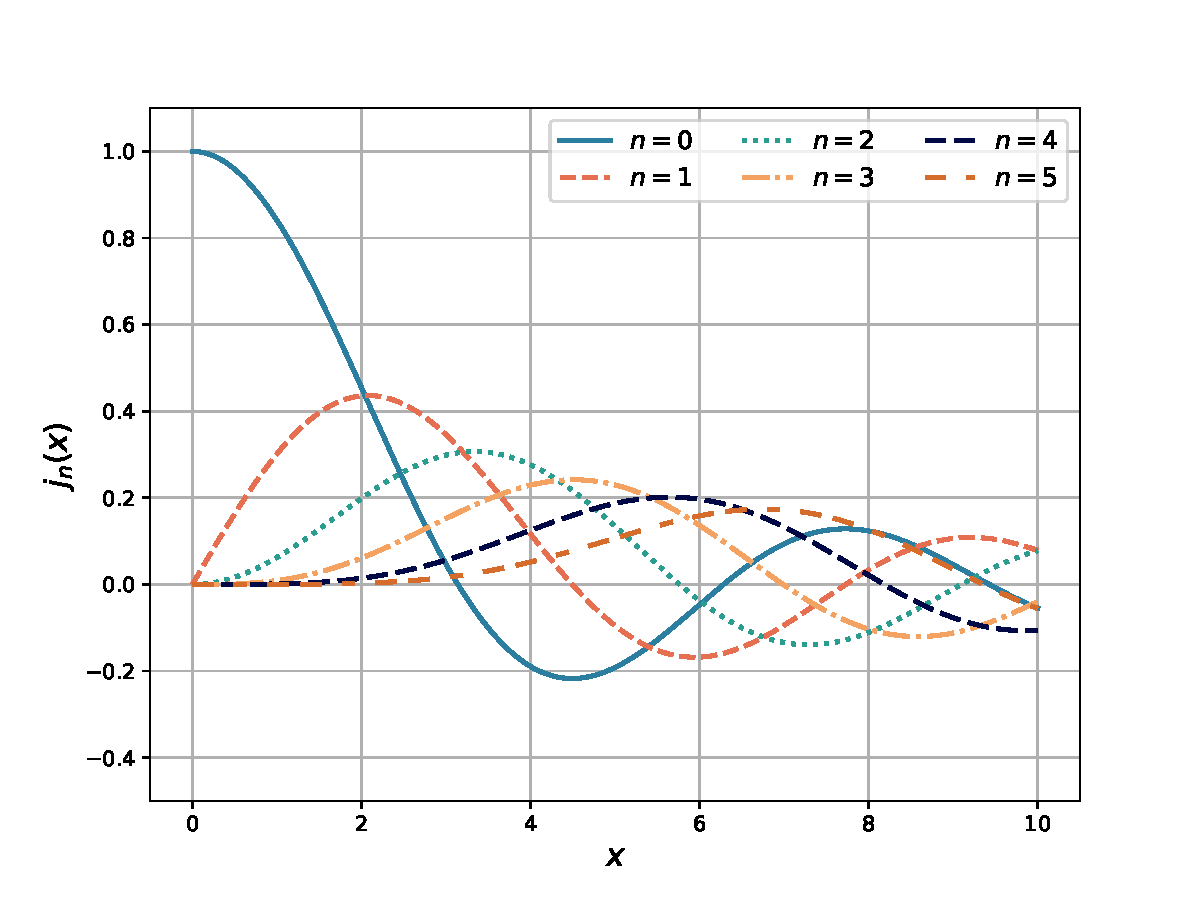
\includegraphics[width = 12cm]{Figuras/Bessel-Esferica-first-kind.pdf}
    \caption{Funciones esféricas de Bessel de orden entero para $n$ entre 0 y 5. Adaptación de \href{https://github.com/gfrubi/FM2/blob/master/figuras-editables/fig-Bessel.py}{este} código. La adaptación se encuentra \href{aa}{aquí}.}
    \label{fig:esferica_bessel_primera}
\end{figure}

\begin{figure}[htbp]
    \centering
    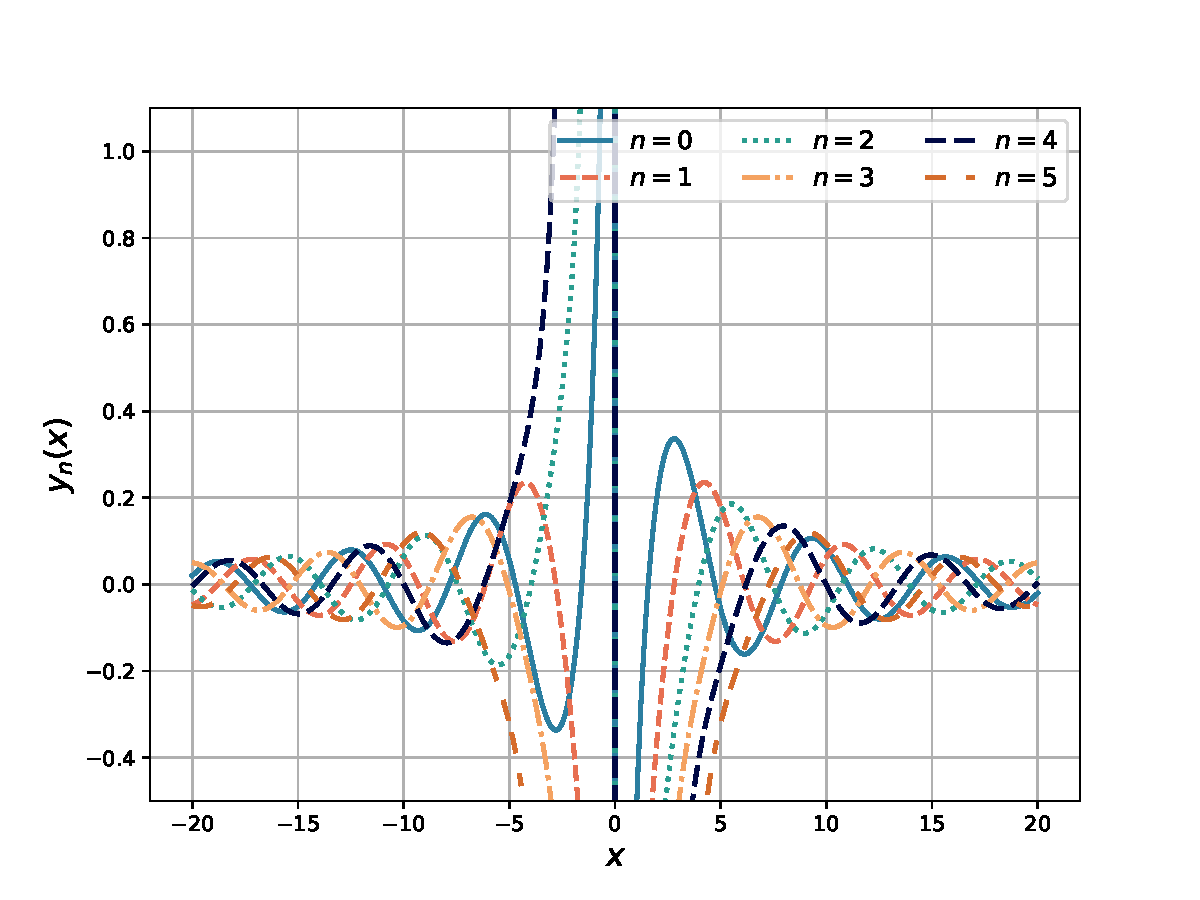
\includegraphics[width = 12cm]{Figuras/Bessel-Esferica-second-kind.pdf}
    \caption{Funciones esféricas de Neumann de orden entero para $n$ entre 0 y 5. Adaptación de \href{https://github.com/gfrubi/FM2/blob/master/figuras-editables/fig-Bessel.py}{este} código. La adaptación se encuentra \href{aa}{aquí}.}
    \label{fig:esferica_bessel_segunda}
\end{figure}

\subsection{Función generatriz (para orden entero)}

Las funciones esféricas de Bessel de orden entero pueden obtenerse a partir de las siguientes funciones generatrices
\begin{align}
    G_j(x,t) & = \frac{1}{x} \cos \left( \sqrt{x^2 - 2xt} \right) = \sum_{n=0}^\infty \frac{t^n}{n!} j_{n-1}(x) \ , \\
    G_y(x,t) & = \frac{1}{x} \sin \left( \sqrt{x^2 - 2xt} \right) = \sum_{n=0}^\infty \frac{t^n}{n!} y_{n-1}(x) \ .
\end{align} 

\subsection{Ceros de las funciones esféricas de Bessel}

Al igual que en el caso de las funciones de Bessel, no es posible hallar las raíces de las funciones esféricas de Bessel de forma analítica, por lo que en la tabla \ref{tab:alphanun_esferica} presentamos algunos ceros para funciones de orden entero. A su vez, en la tabla \ref{tab:betanun_esferica} presentamos los ceros de su primera derivada.

\begin{table}[htbp]
    \centering
    \begin{tabular}{ccccccc}
    \hline $\alpha_{n,p}$ & $n=1$ & $n=2$ & $n=3$ & $n=4$ & $n=5$ \\ \hline 
    $\nu=0$ & 3.1416 &  6.2832 &  9.4248 & 12.5664 & 15.7080 \\
    $\nu=1$ & 4.4934 &  7.7253 & 10.9041 & 14.0662 & 17.2208 \\
    $\nu=2$ & 5.7635 &  9.0950 & 12.3229 & 15.5146 & 18.6890 \\
    $\nu=3$ & 6.9879 & 10.4171 & 13.6980 & 16.9236 & 20.1218 \\
    $\nu=4$ & 8.1826 & 11.7049 & 15.0397 & 18.3013 & 21.5254 \\
    \hline 
    \end{tabular} 
    \caption{Las primeras raíces $\alpha_{n,p}$ de $j_n(x)$, $n=0,1,2,3,4$. Valores tomados del capítulo 14 de \cite{Arfken}.}
    \label{tab:alphanun_esferica}
\end{table}

\begin{table}[htbp]
    \centering
    \begin{tabular}{ccccccc}
    \hline $\beta_{n,p}$ & $n=1$ & $n=2$ & $n=3$ & $n=4$ & $n=5$ \\ \hline 
    $\nu=0$ & 4.4934 & 7.7253 & 10.9041 & 14.0662 & 17.2208 \\
    $\nu=1$ & 2.0816 & 5.9404 &  9.2058 & 12.4044 & 15.5792 \\
    $\nu=2$ & 3.3421 & 7.2899 & 10.6139 & 13.8461 & 17.0429 \\
    $\nu=3$ & 4.5141 & 8.5838 & 11.9727 & 15.2445 & 18.4681 \\
    $\nu=4$ & 5.6467 & 9.8404 & 13.2956 & 16.6093 & 19.8624 \\
    \hline 
    \end{tabular} 
    \caption{Las primeras raíces $\beta_{n,p}$ de $j'_n(x)$, $n=0,1,2,3,4$. Valores tomados del capítulo 14 de \cite{Arfken}.}
    \label{tab:betanun_esferica}
\end{table}

\subsection{Propiedades}

\begin{propiedad}
    \textbf{Propiedades de las funciones esféricas de Bessel.}

    \begin{enumerate}
        \item \textbf{Ortogonalidad respecto a las raíces.} A partir de la ortogonalidad de las funciones de Bessel, tenemos que
        \begin{equation}
            \int_0^a j_n\left( \alpha_{n,p} \frac{x}{a} \right) j_n\left( \alpha_{n,q} \frac{x}{a}  \right) r^2 \ dr = \frac{a^3}{2} \left[ j_{n+1}(\alpha_{np}) \right]^2 \delta_{pq} \ .
        \end{equation}
        \item \textbf{Ortogonalidad respecto al orden.} Tenemos que, a diferencia de las funciones de Bessel, las funciones esféricas de Bessel son ortogonales respecto a su orden, tal que
        \begin{equation}
            \int_{-\infty}^{+\infty} j_m(x) j_n(x) dx = \frac{\pi}{2n+1} \delta_{mn} \ .
        \end{equation}
        \item \textbf{Funciones esféricas de Hankel.} De forma análoga a las funciones de Bessel, podemos definir las funciones esféricas de Hankel como
        \begin{align}
            h_\ell^{(1)}(x) & = \sqrt{\frac{\pi}{2x}}H_{\ell + 1/2}^{(1)}(x) = j_n(x) + i y_n(x) \ , \\
            h_\ell^{(2)}(x) & = \sqrt{\frac{\pi}{2x}}H_{\ell + 1/2}^{(2)}(x) = j_n(x) - i y_n(x) \ .
        \end{align}
        \item \textbf{Expansión en serie de potencias.} Para el caso de orden entero, es posible representar las funciones esféricas de Bessel en términos de una serie de potencias, donde
        \begin{align}
            j_n(x) & = 2^n x^n  \sum_{k=0}^\infty \frac{(-1)^k}{k!} \frac{(k+n)!}{(2k+2n+1)!}x^{2k} \ , \\
            y_n(x) & = \frac{(-1)^{n+1}}{2^n x^{n+1}} \sum_{k = 0}^\infty \frac{(-1)^k (k-n)!}{k! (2k-2n)!}z^{2k} \ .
        \end{align}
        \item \textbf{Comportamiento asintótico.} A partir del comportamiento asintótico de las funciones de Bessel, tenemos que
        \begin{align}
            j_n(x) & \approx \frac{1}{x} \sin\left( x - \frac{n\pi}{2} \right) \ , \\
            y_n(x) & \approx - \frac{1}{x} \cos\left( x - \frac{n\pi}{2} \right) \ , \\
            h_n^{(1)}(x) = H_n^{(2)}(x)^\ast & = \approx (-i)^{n+1} \frac{e^{ix}}{x} = - \frac{e^{i(x-n\pi/2)}}{x} \ .
        \end{align}
        \item \textbf{Relaciones de recurrencia.} Cualquier función esférica de Bessel satisface las relaciones de recurrencia
        \begin{align}
            f_{n-1}(x) + f_{n+1}(x) & = \frac{2n+1}{x} f_n(x) \ , \\
            n f_{n-1}(x) - (n+1) f_{n+1}(x) & = (2n+1) f'_n(x) \ .
        \end{align}
        \item \textbf{Relaciones con derivadas.} Las funciones esféricas de Bessel de orden $n$ pueden obtenerse a partir de las funciones de orden 0 mediante sucesivas derivaciones, esto es,
        \begin{align}
            j_n(x) & = (-1)^n x^n \left( \frac{1}{x} \frac{d}{dx} \right)^n \left( \frac{\sin x}{x} \right) \ , \\
            y_n(x) & = (-1)^n x^n \left( \frac{1}{x} \frac{d}{dx} \right)^n \left( \frac{\cos x}{x} \right) \ , \\
            h_n^{(1)}(x) & = -i (-1)^n x^n \left( \frac{1}{x} \frac{d}{dx} \right)^n \left( \frac{e^{ix}}{x} \right) \ , \\
            h_n^{(2)}(x) & = i (-1)^n x^n \left( \frac{1}{x} \frac{d}{dx} \right)^n \left( \frac{e^{-ix}}{x} \right) \ .
        \end{align}
        \item \textbf{Funciones esféricas modificadas de Bessel.} Puede darse el caso en que la ecuación esférica de Bessel tenga la forma de la ecuación modificada de Bessel para orden $1/2$. En ese caso,se definen las \emph{funciones esféricas de Bessel modificadas} como
        \begin{align}
            i_n(x) & = \sqrt{\frac{\pi}{2x}} I_{n+1/2}(x) \ , \\
            k_n(x) & = \sqrt{\frac{2}{\pi x}} K_{n+1/2}(x) \ .
        \end{align} 
        Nótese que el factor de escala para $k_n$ es diferente al utilizado para el resto de las funciones esféricas de Bessel.
    \end{enumerate}
\end{propiedad}



% Nuevamente, podemos hacer uso del método de Frobenius para resolver la EDO alrededor de $x=0$. Podríamos preguntarnos si esto es posible, ya que $x=0$ corresponde a un punto singular de la ecuación, ya que si consideramos una solución de la forma $y(x) = \sum_n a_n x^n$, en $x=0$, $y(0) = 0$

\begin{ejemplo}
    \textbf{(Arfken 7$^{\boldsymbol{\circ}}$ Edición, Ejemplo 14.7.1)} Considere una partícula cuántica libre de masa $m$ y con energía $E$ que se mueve dentro de una esfera de radio $a$. Encuentre el valor mínimo de energía para el cual la función de onda del sistema tiene una solución física. Para esto, considere que
    \begin{enumerate}
        \item La función de onda $\psi(r)$ es finita dentro de la esfera, es decir, para $0 \leq r \leq a$.
        \item En los bordes de la esfera, $\psi(a) = 0$.
    \end{enumerate} 

    \textbf{Solución.} Esta situación puede ser descrita mediante la ecuación de Schrödinger independiente del tiempo,
    \begin{equation*}
        - \frac{\hbar^2}{2m} \nabla^2 \psi = (E - V(r)) \psi \ ,
    \end{equation*}
    donde podemos modelar el potencial como un pozo cuadrado, tal que
    \begin{equation*}
        V(r) = \left\{ \begin{array}{cc}
            0 \ , & \quad r \leq a \ , \\
            \infty \ , & \quad r > a \ .
        \end{array} \right.
    \end{equation*}
    Luego, en el interior de la esfera, la ecuación de Schrödinger correspondiente será
    \begin{equation*}
        - \frac{\hbar^2}{2m} \nabla^2 \psi = E \psi \ .
    \end{equation*}
    
    Realizamos separación de variables, obteniendo la ecuación radial
    \begin{equation*}
        \frac{d^2R}{dr^2} + \frac{2}{r} \frac{dR}{dr} + \left[ k^2 - \frac{\ell(\ell+1)}{r^2} \right]R = 0 \ ,
    \end{equation*}
    que corresponde a la ecuación esférica de Bessel, con $k^2 = 2mE/\hbar^2$. Así, la solución general para $R$ será dada por
    \begin{equation*}
        R(r) = A j_\ell(kr) + By_\ell(kr) \ .
    \end{equation*}
    Descartamos la presencia de las funciones de segunda especie, pues estas no son finitas en $r = 0$, para lo cual imponemos que $B = 0$. Por otra parte, imponiendo la condición de borde $\psi(a) = R(a) = 0$, necesitamos que $j_\ell(ka) = 0$, de donde concluimos que
    \begin{equation*}
        k = \frac{\alpha_{\ell,i}}{a} \ ,
    \end{equation*}
    donde $\alpha_{\ell,i}$ es la $i$-ésima raíz positiva de $j_\ell$. Luego, la solución para la ecuación radial tendrá la forma
    \begin{equation*}
        R(r) = A j_\ell \left( \frac{\alpha_{\ell,i}}{a} r \right) \ .
    \end{equation*}

    De la definición de $k^2$, observamos que el menor valor de energía se corresponderá con el menor valor de $k^2$, que a su vez corresponderá a la primera raíz positiva de $j_\ell$, siendo esta la que corresponde para $\ell = 0$. De la tabla \ref{tab:alphanun_esferica}, observamos que esta corresponde a $\alpha_{0,1} \approx 3.1416 = \pi$, de modo que el menor valor de energía posible corresponde a
    \begin{equation*}
        E_{\min} = \frac{\hbar^2 k_{\min}^2}{2m} = \frac{\hbar^2}{2m} \left(\frac{\pi}{a}\right)^2 = \frac{\pi^2 \hbar^2}{2ma^2} = \frac{h^2}{8ma^2} \ .
    \end{equation*}

    Para finalizar, algunas observaciones,
    \begin{itemize}
        \item Esta \emph{energía mínima posible} es comúnmente denominada energía del \textbf{estado fundamental}, \textbf{estado basal} o \textbf{\emph{groundstate}}, o bien \textbf{energía del punto cero}. Por ejemplo, el átomo de hidrógeno posee una energía mínima $E_{\min} = -13.6$ eV.
        
        \item La energía de este sistema \emph{cuántico} no es continua, sino que solo puede tomar valores discretos, correspondientes a autovalores de la ecuación de Schrödinger.
        
        \item Para cualquier partícula encerrada dentro de una esfera, el valor mínimo de energía siempre será positivo.

        \item En este ejemplo, la energía mínima dependerá del valor de $\ell$, de modo que si deseamos encontrar la energía mínima del $\ell$-ésimo estado, esta será dada por
        \begin{equation*}
            E_{\ell_{\min}} = \frac{\hbar^2 \alpha_{\ell, 1}}{2ma^2} \ .
        \end{equation*}
    \end{itemize}
\end{ejemplo}
\chapter{Funciones de Green}

Hasta ahora, hemos visto maneras de resolver EDPs lineales y \emph{homogéneas}, es decir, que son igualables a cero, sin términos que no dependan de la función incógnita ni sus derivadas.

Sin embargo, muchas situaciones físicas no pueden ser descritas únicamente mediante ecuaciones homogéneas. ¿Cómo podemos resolverlas en este caso?

Una forma de hacerlo es mediante el \textbf{método de las funciones de Green}, gracias a las cuales podemos reducir una EDP lineal e inhomogénea a un problema abordable.

% En general, diremos que podemos hacer uso de las funciones de Green cuando tenemos un problema de la forma
% \begin{equation}
%     \mathcal{L}\Psi(\vec{x}) = f(\vec{x}) \ ,
% \end{equation}
% donde $f(\vec{x})$ corresponde a una función \emph{fuente} y $\mathcal{L}$ es un operador diferencial cualquiera. 
\begin{defi} \marginnote{Función de Green}
    Dado un operador diferencial $\mathcal{L}$ cualquiera, y una función \emph{fuente} $f(\x)$, tales que
    \begin{equation}
        \mathcal{L}\Psi(\vec{x}) = f(\vec{x}) \ .
    \end{equation}

    Una \textbf{función de Green} $G(\x, \x')$ para el operador $\mathcal{L}$ es aquella que satisface la ecuación
    \begin{equation}\label{eq:condicion_green}
        \mathcal{L}G(\vec{x}, \vec{x}') = \delta^{(n)}(\vec{x} - \vec{x}') \ ,
    \end{equation}
    donde $\delta^{(n)}$ es la delta de Dirac $n$-dimensional.
\end{defi}

\begin{propiedad} \marginnote{Condición de consistencia}
    \textbf{Condición de consistencia.} Integrando la definición de las funciones de Green \eqref{eq:condicion_green} sobre el volumen $V$ en el que se encuentre definida nuestro operador diferencial $\mathcal{L}$, la función de Green cumplirá que
    \begin{equation} \label{eq:condicion_consistencia}
        \int_V \mathcal{L} G(\x, \x') dV = \int_V \delta^{(n)}(\x - \x') dV = 1 \ , \quad \forall \ \x \in V \ .
    \end{equation}
\end{propiedad}
% En este caso, buscamos una \textbf{función de Green} $G(\vec{x}, \vec{x}')$ que satisfaga la ecuación
% \begin{equation}\label{eq:condicion_green}
%     \mathcal{L}G(\vec{x}, \vec{x}') = \delta^{(n)}(\vec{x} - \vec{x}') \ ,
% \end{equation}
% donde $\delta^{(n)}$ es la delta de Dirac $n$-dimensional.

\section{Motivación: Potencial electrostático}

En presencia de una carga (o distribución de cargas), el potencial electrostático satisface la \emph{ecuación de Poisson}
\begin{equation}
    \nabla^2 \phi = - \frac{\rho(x)}{\varepsilon_0} \ ,
\end{equation}
donde $\rho(x)$ es la distribución de cargas en la región considerada.

A partir de la ley de Coulomb, sabemos que podemos describir el potencial eléctrico de una distribución de cargas como
\begin{equation} \label{eq:potencial_coulomb}
    \phi(\vec{x}) = \frac{1}{4\pi \varepsilon_0} \int_V \frac{\rho(\vec{x}')}{|\vec{x} - \vec{x}'|} dV' \ ,
\end{equation}
donde hemos hecho la elección tradicional de que el potencial de referencia se anula en el infinito.

Observamos que, si definimos nuestra \emph{función de Green} como
\begin{equation}\label{eq:green_laplaciano} \marginnote{Función de Green para el Laplaciano}
    G(\vec{x}, \vec{x}') = - \frac{1}{4\pi} \frac{1}{|\vec{x} - \vec{x}'|} \ ,
\end{equation}
podemos reescribir \eqref{eq:potencial_coulomb} como
\begin{equation}
    \phi(x) = \int_V G(\vec{x}, \vec{x}') \left( - \frac{\rho(\vec{x}')}{\varepsilon_0} \right) dV' \ .
\end{equation}

Esta función de Green debe satisfacer la ecuación \eqref{eq:condicion_green}, que en este caso es dada por
\begin{equation}
    \nabla^2 G(\vec{x}, \vec{x}') = \delta^{(3)} (\vec{x} - \vec{x}') \ .
\end{equation}

De esta forma, observamos que
\begin{align}
    \nabla^2 \phi(\vec{x}) & = \nabla^2 \int_V G(\vec{x}, \vec{x}') \left( - \frac{\rho(\vec{x}')}{\varepsilon_0} \right) dV' \\
    & = \int_V [\nabla^2 G(\vec{x}, \vec{x}')] \left( - \frac{\rho(\vec{x}')}{\varepsilon_0} \right) dV' \\
    & = \int_V \delta^{(3)}(\vec{x} - \vec{x}') \left( - \frac{\rho(\vec{x}')}{\varepsilon_0} \right) dV'\\
    & = - \frac{\rho(\vec{x})}{\varepsilon_0} \ ,
\end{align}
recuperando la ecuación original.

\section{Encontrando soluciones mediante funciones de Green}

Consideremos una EDP \emph{lineal e inhomogénea} de la forma
\begin{equation}\label{eq:edp_general}
    \mathcal{L} \psi(\vec{x}) = \left(\nabla \cdot (p(\vec{x}) \nabla) + q(\vec{x})\right)\psi(\vec{x}) = f(\vec{x}) \ ,
\end{equation}
donde $p(\vec{x})$ y $q(\vec{x})$ son funciones conocidas.

Para resolver la EDP, encontramos primero la función de Green que satisface la expresión \eqref{eq:condicion_green}, junto a una solución \emph{particular} de la ecuación \eqref{eq:edp_general} en el punto $\vec{x}'$, podemos hallar una solución general del problema, la que será dada por
\begin{equation}\label{eq:solucion_green}
    \psi(\vec{x}) = \oint_{\partial V} p(\vec{x})[\psi(\vec{x}') \nabla' G(\vec{x}, \vec{x}') - G(\vec{x}, \vec{x}') \nabla' \psi(\vec{x}')] \cdot d\vec{S}' + \int_V G(\vec{x}, \vec{x}') f(\vec{x}') dV' \ ,
\end{equation}
donde $\nabla'$ indica que el operador actúa sobre las componentes de $\vec{x}'$. Aquí, $V$ denota al dominio en que la solución $\psi(\vec{x})$ es válida, y $\partial V$ es su frontera.

¿Cómo sabemos que esta ecuación es válida? Resolvamos la primera integral. Notemos que podemos utilizar el teorema de Gauss, de modo que
\begin{align}
    I & = \oint_{\partial V} p(\vec{x})[\psi(\vec{x}') \nabla' G(\vec{x}, \vec{x}') - G(\vec{x}, \vec{x}') \nabla' \psi(\vec{x}')] \cdot d\vec{S}' \label{eq:integral_green_superficie} \\
    & = \int_V \nabla' \cdot \left[ p(\vec{x}') \psi(\vec{x}') \nabla' G(\vec{x}, \vec{x}') - p(\vec{x}') G(\vec{x}, \vec{x}') \nabla' \psi(\vec{x}') \right] dV' \\
    & = \int_V \left[\psi(\vec{x}') \nabla' \cdot \left[ p(\vec{x}')  \nabla' G(\vec{x}, \vec{x}')\right] + \textcolor{blue}{\nabla \psi(\vec{x}') \cdot (p(\vec{x}') \nabla' G(\vec{x}, \vec{x}') )} \right. \nonumber \\
    & \qquad \quad \left. -  G(\vec{x}, \vec{x}') \nabla' \cdot \left[p(\vec{x}') \nabla' \psi(\vec{x}')\right] \textcolor{blue}{- \nabla \psi(\vec{x}') \cdot (p(\vec{x}') \nabla' G(\vec{x}, \vec{x}') )} \right] dV' \\
    & = \int_V \left[ \psi(\vec{x}') \left( \mathcal{L}' G(\vec{x}, \vec{x}') \right) - G(\vec{x}, \vec{x}') \left( \mathcal{L}' \psi(\vec{x}') \right) \right] dV' \\
    & = \int_V \left[ \psi(\vec{x}') \delta(\vec{x} - \vec{x}') - G(\vec{x}, \vec{x}') f(\vec{x}') \right] dV' \\
    & = \psi(\vec{x}) - \int_V G(\vec{x}, \vec{x}') f(\vec{x}') dV' \ ,
\end{align}
donde hemos definido un nuevo operador diferencial $\mathcal{L}'$ que actúa sobre las componentes primadas, tal que $\mathcal{L}' \psi(\vec{x}') = f(\vec{x}')$.

¿Cómo hallamos una solución en el punto $\vec{x}'$? Haciendo uso de las condiciones de borde del problema, que usualmente serán definidas en el contorno $\partial V$.

\subsection{Condiciones de borde de tipo Dirichlet}

Si las condiciones de borde son \emph{de tipo Dirichlet}, sabemos el valor de $\psi(\vec{x}')$ en el borde $\partial V$ de la región en que nos encontramos, por lo que podremos determinar el primer término de la integral sobre $\partial V$ en \eqref{eq:integral_green_superficie}, pero el segundo, que depende de la derivada de $\psi(\vec{x}')$, no estará determinado. Por ello, escogeremos \emph{de forma conveniente} una función de Green que se anule en los bordes, es decir,
\begin{equation}\label{eq:condicion_dirichlet_green}
    G(\vec{x}, \vec{x}') = 0 \ , \qquad \forall \ \vec{x}' \in \ \partial V \ .
\end{equation}

En este caso, la solución general tendrá la forma
\begin{equation}\label{eq:solucion_dirichlet}
    \psi(\vec{x}) = \int_V G(\vec{x}, \vec{x}') f(\vec{x}') dV + \oint_{\partial V} p(\vec{x}') \psi(\vec{x}') \frac{\partial G(\vec{x}, \vec{x'})}{\partial n'} dS' \ ,
\end{equation}
donde $\partial f/\partial n' = (\nabla' f) \cdot \hat{n}$ , con 
$\hat{n}$ un vector normal a la superficie.

Sin embargo, muchas veces puede ser difícil hallar directamente una función de Green que satisfaga a la vez \eqref{eq:condicion_dirichlet_green} y \eqref{eq:condicion_green}. Un ejemplo sencillo de esto es el operador laplaciano, cuando $\mathcal{L} = \nabla^2$. En este caso, es útil buscar una solución de la forma
\begin{equation}\label{eq:green_fundamental}
    G(\x, \x') = F(\x, \x') + H(\x, \x') \ ,
\end{equation}
donde $F(\x, \x')$ satisface la ecuación \eqref{eq:condicion_green} pero no necesariamente la condición de borde \eqref{eq:condicion_dirichlet_green}, mientras que $H(\x, \x')$ satisface la ecuación \emph{homogénea del problema} (es decir, donde no hay funciones fuente) en el interior de la región $V$, pero su valor en $\partial V$ es tal que, sumada a $F(\x, \x')$, resulta en que $G(\x,\x') = 0$ en el borde $\partial V$. Cuando seguimos este procedimiento, la función $F(\x,\x')$ es denominada \textbf{solución fundamental}. En efecto,
\begin{equation}
    \nabla^2 G(\x, \x') = \nabla^2 F(\x, \x') + \nabla^2 H(\x, \x') = \nabla^2 F(\x, \x') + 0 = \delta^{(3)}(\x - \x') \ .
\end{equation}

\begin{ejemplo}
    \textbf{(Riley, Sección 21.5.3)} Encuentre la solución fundamental a la ecuación de Poisson en tres dimensiones, sujeta a la condición de contorno $F(\x , \x') \to 0$ cuando $|\x| \to \infty$.

    \textbf{Solución.}  Dado que nuestro contorno se encuentra en infinito, el problema posee simetría esférica, y puede ser modelado como una esfera $S$ de radio $R$ \emph{muy grande} centrada en $\x'$. La condición de consistencia \eqref{eq:condicion_consistencia} establece
    \begin{equation*}
        \int_V \nabla^2 F(\x, \x') dV = \int_V \delta^{(3)}(\x-\x') dV = 1 \ ,
    \end{equation*}
    que a su vez, usando el teorema de Gauss, puede escribirse como
    \begin{equation}
        \int_S \nabla F(\x, \x') \cdot d\vec{S}' = 1 \ .
    \end{equation}

    Dada la simetría esférica del problema, podemos suponer que nuestra función dependa únicamente de la distancia entre el centro y el punto $\x$, de modo que $F(\x,\x') = F(|\x-\x') = F(r)$. Evaluando la integral de superficie, tenemos que
    \begin{equation*}
        4\pi r^2 \left. \frac{dF}{dr}\right|_{r=R} = 1 \ .
    \end{equation*}

    Integrando sobre $r$, podemos encontrar una expresión para $F$, de modo que
    \begin{equation*}
        F(r) = - \frac{1}{4\pi r} + C \ ,
    \end{equation*}
    que sumado a la condición de contorno del problema, deducimos que $C = 0$. Luego, la solución fundamental en tres dimensiones es dada por
    \begin{equation*}
        F(\x, \x') = - \frac{1}{4\pi |\x-\x'|} \ .
    \end{equation*}
\end{ejemplo}

\subsection{Condiciones de borde de tipo Neumann}


Si las condiciones de borde son \textbf{de tipo Neumann}, conocemos el valor de la derivada $\frac{\partial \psi}{\partial n}(\vec{x}')$ en el borde $\partial V$ de la región en que nos encontramos, por lo que podemos determinar el segundo término de la integral \eqref{eq:integral_green_superficie}, mas no así el primero. 

Por analogía al caso de las condiciones de Dirichlet, podríamos pensar en escoger una función de Green que satisfaga
\begin{equation} \label{eq:condicion_neumann_green}
    \frac{\partial G(\vec{x}, \vec{x}')}{\partial n'} = 0 \ , \qquad \forall \ \vec{x}' \in \ \partial V \ ,
\end{equation}
con lo que la solución general tendría la forma
% En este caso, la solución general tendrá la forma
\begin{equation}\label{eq:solucion_neumann_inicial}
    \psi(\x) = \int_V G(\x, \x') f(\x') dV - \oint_{\partial V} p(\x ') G(\x, \x') \frac{\partial \psi(\x')}{\partial n'} dS' \ .
\end{equation}

Lamentablemente, en general \emph{no es posible} encontrar una función de Green que satisfaga la condición \eqref{eq:condicion_neumann_green}, siendo nuevamente un ejemplo de esto el operador laplaciano $\nabla^2$, ya que las funciones de Green deben satisfacer la condición de consistencia \eqref{eq:condicion_consistencia}. Por ello, ya que descartamos la solución más sencilla posible ($\frac{\partial G(\vec{x}, \vec{x}')}{\partial n'} = 0$), escogemos la segunda más sencilla, igualar la derivada a una constante,
\begin{equation}
    \frac{\partial G(\vec{x}, \vec{x}')}{\partial n'} = C \ , \qquad \forall \vec{x}' \in \ \partial V \ .
\end{equation}
Para hallar el valor de esta constante, hacemos uso de la \emph{condición de consistencia}, de modo que el caso más sencillo será suponer que $C = 1/\text{Área}(\partial V)$.

De ser posible esta elección, la solución tendrá la forma
\begin{equation}\label{eq:solucion_neumann}
    \psi(\x) = \int_V G(\x, \x') f(\x') dV - \oint_{\partial V} p(\x ') G(\x, \x') \frac{\partial \psi(\x')}{\partial n'} dS' + \underbrace{\frac{1}{A} \oint_{\partial V} p(\x) \psi(\x') \ dS'}_{\langle \psi(\x') \rangle_{\partial V}} \ .
\end{equation}
Aquí, la notación $\langle \psi(\x') \rangle_{\partial V}$ representa una especie de \emph{valor promedio ponderado} sobre el contorno $\partial V$. Este promedio actuará como una constante que puede ser determinada libremente. Es más, si el contorno $\partial V$ de la región es el infinito, este término puede ser fijado a cero, pues no requeriremos de este término para que la solución tenga sentido físico.

% \begin{ejemplo}
%     \textbf{(Riley, Sección 21.5.4)} Resuelva la ecuación de Laplace en la región bidimensional $|\x| \leq a$ sujeta a la condición de contorno $\partial \Psi/\partial n = f(\phi)$ en $|\x| = a$. Considere que la condición de consistencia implica que $\int_0^{2\pi} f(\phi) d\phi = 0$.

%     \textbf{Solución.} 
% \end{ejemplo}

\begin{obs}{Observación}
    Es importante recordar que una misma EDP puede dar origen a diferentes funciones de Green, pues estas dependen también de las condiciones de contorno.
\end{obs}


\section{Simetría de las funciones de Green}

Cuando tenemos el caso particular en que $\mathcal{L} = \nabla^2$, la función de Green \eqref{eq:green_laplaciano} es simétrica bajo el intercambio de argumentos, es decir, $G(\x, \x') = G(\x', \x)$. Podemos buscar cuál es la condición general que permite que esto ocurra, escogiendo $\psi(\x) = \psi(\x'', \x)$, de modo que, según la expresión \eqref{eq:solucion_green},
\begin{align}
    \nonumber G(\x'', \x) & = \int_V G(\x, \x') \delta(\x'' - \x') dV' \\ 
    & \qquad + \oint_{\partial V} p(\x')\left[ G(\x'', \x') \nabla' G(\x, \x') - G(\x, \x') \nabla'G(\x'', \x') \right] \cdot d\vec{S}' \\
    & = G(\x, \x'') + \oint_{\partial V} p(\x')\left[ G(\x'', \x') \nabla' G(\x, \x') - G(\x, \x') \nabla'G(\x'', \x') \right] \cdot d\vec{S}' \ ,
\end{align}
con lo que vemos que la función de Green será simétrica siempre y cuando la integral de superficie se anule en la frontera, 
\begin{equation}\label{eq:condicion_simetria}
    \oint_{\partial V} p(\x')\left[ G(\x'', \x') \nabla' G(\x, \x') - G(\x, \x') \nabla'G(\x'', \x') \right] \cdot d\vec{S}' = 0 \ .
\end{equation}
% Esto ocurre, típicamente, para condiciones de tipo Dirichlet.
A continuación, listamos algunas situaciones en que una función de Green será simétrica.

\begin{propiedad}
    \textbf{Simetría de las funciones de Green.} Una función de Green para un operador diferencial $\mathcal{L}$ será simétrica, esto es, $G(\x, \x') = G(\x', \x)$, si 
    \begin{enumerate}
        \item El problema posee condiciones de tipo Dirichlet homogéneas.
        \item El problema posee condiciones de tipo Neumann homogéneas.
        \item El operador diferencial es \emph{hermítico}, esto es, $\mathcal{L} = \mathcal{L}^\dagger$.
        \item El operador diferencial es \emph{real}, ya que no poseerá parte imaginaria por conjugar.
        \item Cualquier otra condición que satisfaga la expresión \eqref{eq:condicion_simetria}.
    \end{enumerate}
\end{propiedad}

\section{Método de las imágenes}

Anteriormente mencionamos que podemos hallar la función de Green para un problema con condiciones de Dirichlet hallando la solución fundamental y una solución que produzca que $G(\x,\x') = 0$ en $\partial V$, como establecimos en \eqref{eq:green_fundamental}. Para ello, podemos hacer uso del \textbf{método de las imágenes}, en el cual hemos de considerar \emph{copias} de nuestra solución fundamental que representen \emph{fuentes} ubicadas en el exterior de nuestra región $V$. Este método es de gran utilidad en problemas de electrostática que presenten geometrías altamente simétricas, y será aplicado en este contexto en el curso de Electrodinámica I.
\begin{propo} \marginnote{Método de las imágenes}
    \textbf{Método de las imágenes.} Es posible hallar una función de Green para una ecuación inhomogénea al sumar a la solución fundamental $F(\x, \x')$ diferentes copias (o \emph{imágenes}) de la ella misma, ubicadas \emph{fuera} de la región $V$ en la que deseamos resolver la ecuación. Para ello, seguiremos el siguiente procedimiento,
    \begin{enumerate}
        \item Para una fuente singular $\delta(\x - \x')$ dentro de la región $V$, añadiremos fuentes imágenes \emph{fuera} de $V$, donde las posiciones $\x_n$ e intensidades $q_n$ de estas fuentes las podremos determinar a futuro, de modo que las fuentes externas se pueden expresar como
        \begin{equation}
            \sum_{n=1}^N q_n \delta(\x - \x_n) \ , \qquad \x_n \notin \ V \ .
        \end{equation}
    
        \item Ya que todas las imágenes se encuentran en el exterior de $V$, la solución fundamental que corresponde a cada una de las fuentes deberá satisfacer la ecuación de Laplace \emph{dentro} de $V$. Por ello, podemos suponer que cada imagen tiene asociada la misma \emph{solución fundamental} que la fuente en el interior de $V$, con lo que la función de Green tomará la forma
        \begin{equation}
            G(\x, \x') = F(\x, \x') + \sum_{n=1}^N q_n F(\x,\x_n) \ .
        \end{equation}
    
        \item Ajustamos las posiciones $\x_n$ e intensidades $q_n$ de las imágenes de modo que las condiciones de contorno se satisfagan en $S$. En el caso de las condiciones de Dirichlet, esto es exigir que $G(\x, \x') = 0$, para cualquier $\x' \in \partial V$.
    
        \item Por último, podemos usar la función de Green hallada para encontrar la solución, sujeta a las condiciones de Dirichlet, que satisfaga \eqref{eq:solucion_dirichlet}.
    \end{enumerate}
\end{propo}

En general, no es tarea sencilla encontrar las posiciones e intensidades correctas para cualquier problema, pero sí lo es para ciertos problemas con geometrías simples. Particularmente, este método es útil para problemas en los que los bordes sean \emph{líneas rectas} (problema bidimensional) o \emph{planos} (problema tridimensional), pues en esos casos simplemente supondremos que estos actúan como espejos, de modo que la fuente \emph{verdadera} se refleja simétricamente en este espejo.

\begin{ejemplo}
    \textbf{(Riley, Sección 21.5.3)} Resuelva la ecuación de Laplace en la región bidimensional $|\x| \leq a$ sujeta a la condición de contorno $u = h(\phi)$ en $|\x| = a$, dada una carga fuente ubicada en $\x_0$.

    \textbf{Solución.} Nuestro problema corresponde a un disco de radio $a$ sujeto a condiciones de Dirichlet. Como queremos que nuestra función de Green satisfaga que $G(\x, \x_0) = 0$ para $|\x| = a$, podemos suponer que nuestra \emph{carga imagen} se encuentra fuera del disco en una posición $\x_1 = (a^2/|\x_0|^2)\x_0$, de modo que, suponiendo que la intensidad de la carga imagen es $-1$, nuestra función de Green toma la forma (véase la siguiente sección para la deducción detallada de la función de Green para el Laplaciano en 2D)
    \begin{equation*}
        G(\x, \x_0) = \frac{1}{2\pi} \ln(|\x - \x_0|) - \frac{1}{2\pi} \ln(|\x - \x_1|) + C \ .
    \end{equation*}

    Del hecho que $G(\x, \x_0) = 0$ para $|\x| = a$, tenemos que
    \begin{align*}
        2\pi C & = \ln(|\x - \x_1|) - \ln(|\x - \x_0|) \\
        & = \ln\left( \frac{|\x - \x_1|}{|\x - \x_0|} \right) \\
        & = \ln \left( \frac{\sqrt{a^4/x_0^2 - 2 a^3 \cos(\phi - \phi_0)/x_0 + a^2}}{|\x - \x_0|} \right) \\
        & = \ln \left( \frac{\sqrt{(a^2/x_0^2)}\cancel{|\x - \x_0|}}{\cancel{|\x - \x_0|}} \right) \\
        & = - \ln \left( \frac{x_0}{a} \right)
        % \\
        % & = \ln\left( \sqrt{\frac{a^2}{x_0^2}} \right) \ ,
    \end{align*}
    donde $x_0 = |\x_0|$. Así,
    \begin{equation*}
        C = - \frac{1}{2\pi} \ln \frac{x_0}{a} \ ,
    \end{equation*}
    y nuestra función de Green toma la forma 
    \begin{equation*}
        G(\x, \x_0) = \frac{1}{2\pi} \left[ \ln|\x - \x_0| - \ln\left| \x - \frac{a^2}{x_0^2} \x_0 \right| - \ln \frac{x_0}{a} \right] \ .
    \end{equation*}

    Conociendo nuestra función de Green, podemos utilizar la ecuación \eqref{eq:solucion_dirichlet} para hallar una solución a nuestro problema. Como trabajamos con la ecuación de Laplace, $f(\x_0) = 0$, de modo que solo sobrevive la integral sobre el contorno de nuestra región en \eqref{eq:solucion_dirichlet}, con lo cual
    \begin{equation*}
        \psi(\x) = \oint_C \psi(\x') \frac{\partial G(\x, \x')}{\partial n'} \ d\ell' = \int_0^{2\pi} \psi(\x') \left. \frac{\partial G}{\partial \rho'}\right|_{\rho' = a} a \ d\phi' \ .
    \end{equation*}

    Para nuestra función de Green,
    \begin{align*}
        \frac{\partial G}{\partial \rho'} & = \hat{x}' \cdot \nabla' G(\x,\x') \\
        & = \hat{x}' \cdot \nabla' G(\x',\x) \\
        & = \frac{\x'}{2\pi x'} \cdot \left( \frac{\x' - \x}{|\x' - \x|^2} - \frac{\x' - (a^2/x^2)\x}{|\x' - (a^2/x^2)\x|^2} \right) \ .
    \end{align*}
    que en $\rho' = a$ satisface que
    \begin{align*}
        \left. \frac{\partial G}{\partial \rho'} \right|_{\rho' = a} & = \frac{\x'}{2\pi a} \cdot \left( \frac{\x' - \x}{|\x' - \x|^2} - \frac{\x' - (a^2/x^2)\x}{(a^2/x^2)|\x' - \x|^2} \right) \\
        & = \frac{\x'}{2\pi a} \cdot \frac{(a^2/x^2)\x' - (a^2/x^2) \x - \x' + (a^2/x^2)\x }{(a^2/x^2)|\x' - \x|^2} \\
        & = \frac{1}{2\pi a} \frac{a^2 - x^2}{|\x' - \x|^2} \\
        & = \frac{1}{2\pi a} \frac{a^2 - \rho^2}{a^2 + \rho^2 - 2a\rho \cos(\phi' - \phi)} \ .
    \end{align*}
    
    De esta manera, concluimos que una solución a nuestro problema puede ser hallada como
    \begin{equation*}
        u(\rho, \phi) = \frac{1}{2\pi} \int_0^{2\pi}  \frac{(a^2 - \rho^2) f(\phi') \ d\phi'}{a^2 + \rho^2 - 2a\rho \cos(\phi' - \phi)} \ .
    \end{equation*}
\end{ejemplo}

También es útil mencionar que es válido utilizar el método de las imágenes al trabajar con condiciones de Neumann, donde el procedimiento descrito anteriormente sigue siendo el mismo, pero utilizando las condiciones de Neumann para establecer nuestras imágenes.

\begin{ejemplo}
    \textbf{(Riley, Sección 21.5.4)} Resuelva la ecuación de Laplace en la región bidimensional $|\x| \leq a$ sujeta a la condición de contorno $\partial u/\partial n = f(\phi)$ en $|\x| = a$, con $\int_0^{2\pi} f(\phi) d\phi = 0$, como requiere la condición de consistencia.

    \textbf{Solución.} La geometría del problema es la misma que la del ejemplo anterior. Por ello, podemos suponer que la carga imagen se encuentra en la misma posición $\x_1 = (a^2/x_0^2) \x_0$, donde nuevamente $\x_0$ corresponde a la carga fuente dentro del círculo. Sin embargo, ahora no asumiremos la intensidad de la carga imagen, sino que la dejaremos como un parámetro $q$. De esta forma, la función de Green será de la forma
    \begin{equation*}
        G(\x, \x_0) = \frac{1}{2\pi} \left( \ln |\x - \x_0| + q \ln |\x - \x_1| + C \right) \ .
    \end{equation*}

    En este caso, la derivada radial (normal) de esta función es dada por
    \begin{equation*}
        \frac{\partial G}{\partial \rho} = \frac{\x}{|\x|} \cdot \nabla G(\x, \x_0) = \frac{\x}{2\pi |\x|} \cdot \left[ \frac{\x - \x_0}{|\x - \x_0|^2} + q \frac{\x - \x_1}{|\x - \x_1|^2} \right] \ ,
    \end{equation*}
    que evaluada en $\rho = a$, tenemos que
    \begin{equation*}
        \left. \frac{\partial G}{\partial \rho} \right|_{\rho = a} = \frac{1}{2\pi a} \frac{1}{|\x - \x_0|^2} \left[ |\x|^2 + qx_0^2 - (1+q) \x \cdot \x_0 \right] \ .
    \end{equation*} 

    Como se discutió anteriormente, en problemas con condiciones de tipo Neumann es conveniente escoger que esta derivada se iguale a alguna constante, típicamente el inverso del valor del ``área'' del contorno de nuestra región. Dado que estamos trabajando en una región bidimensional, esta ``área'' corresponde al perímetro del círculo, de modo que
    \begin{equation*}
        \left. \frac{\partial G}{\partial \rho} \right|_{\rho = a} = \frac{1}{2\pi a} \ ,
    \end{equation*}
    lo que se cumple escogiendo $q = 1$. Así, observamos que para un problema con la misma geometría, las condiciones de contorno afectarán al valor de la intensidad $q$ de la carga imagen.

    Podemos encontrar la solución a nuestro problema a partir de la ecuación \eqref{eq:solucion_neumann}, donde al tratarse de la ecuación de Laplace, $f(x) = 0$, con lo que la solución será de la forma
    \begin{equation*}
        \psi(\x) = \langle \psi(\x) \rangle_{C} - \oint_{\partial V} G(\x', \x) f(\x') \ d\ell' 
    \end{equation*}

    Así, la función de Green adecuada, al ser evaluada en $\rho' = a$, tomará el valor
    \begin{align*}
        G(\x',\x)|_{\rho' = a} & = \frac{1}{2\pi} \left[ \ln |\x' - \x| + \ln |\x' - (a^2/x^2)\x| + C \right] \\
        & = \frac{1}{2\pi} \left[ \ln\left( |\x' - \x| |\x - (a^2/x^2)\x| \right) + C \right] \\
        & = \frac{1}{2\pi} \left[ \ln\left( |\x' - \x|^2 \right) + \ln\frac{a}{x} C \right] \\
        & = \frac{1}{2\pi} \left[ \ln(a^2 + \rho^2 - 2 a \rho \cos(\phi' - \phi)) + \ln \frac{a}{\rho} + C \right] \ ,
    \end{align*}
    donde la constante $C$, es una constante arbitraria. Entonces,
    \begin{align*}
        \psi(\rho, \phi) & = \langle \psi(\x) \rangle_C - \frac{a}{2\pi} \int_0^{2\pi} f(\phi') \ln[a^2 + \rho^2 - 2a\rho \cos(\phi' - \phi)] \ d\phi' \\
        & \qquad - \frac{a}{2\pi} \left(\ln \frac{a}{\rho} + C \right) \int_0^{2\pi} f(\phi') \ d\phi' \\
        & = \langle \psi(\x) \rangle_C - \frac{a}{2\pi} \int_0^{2\pi} f(\phi') \ln[a^2 + \rho^2 - 2a\rho \cos(\phi' - \phi)] \ d\phi' \ ,
    \end{align*}
    donde hemos usado la condición dada en el enunciado, $\int_0^{2\pi} f(\phi) d\phi = 0$. 

\end{ejemplo}


\section{Algunas funciones de Green comunes}

Como mencionamos anteriormente, las funciones de Green no son únicas, sino que pueden construirse siempre a partir de una solución fundamental $F(\x,\x')$ que también es una función de Green, sumada a una función $H(\x,\x')$ que es solución al problema homogéneo asociado al operador $\mathcal{L}$,
\begin{equation}
    \mathcal{L} H(\x,\x') = 0 \ .
\end{equation} 

Por ello, listamos a continuación las soluciones fundamentales para el operador Laplaciano y para el Operador de Helmholtz, a las que podemos sumar soluciones a la ecuación homogénea de modo que la suma satisfaga las condiciones de borde del problema específico que podamos estar desarrollando.

\subsection{Ecuación de Laplace}

En este caso, nuestro operador diferencial corresponde a $p(x) = 1$ y $q(x) = 0$ en la definición \eqref{eq:edp_general}. Dado que este curso se centra en métodos útiles en problemas físicos, consideraremos siempre la función de Green que respete la \emph{homogeneidad e isotropía del espacio}, es decir, que la función de Green dependa únicamente de la \emph{diferencia} entre $\x$ y $\x'$ (homogeneidad), y en particular, dependa de la \emph{distancia} $|\x - \x'|$ (isotropía, o invariancia bajo rotaciones). Por ello, la función de Green en este caso corresponde a una función de una variable, que podemos llamar $r = |\x - \x'|$.

\subsubsection{Caso tridimensional}

En un sistema de coordenadas esféricas centradas en $\x'$, nuestra función de Green satisface
\begin{equation}
    \nabla^2 G(r) = \frac{1}{r^2} \frac{d}{dr} \left( r^2 \frac{dG}{dr} \right) = \delta^{(3)}(r) \ ,
\end{equation}
de modo que, si $r \neq 0$, 
\begin{equation}
    \frac{1}{r^2} \frac{d}{dr} \left( r^2 \frac{dG}{dr} \right) = 0 \ .
\end{equation}
Integrando esta expresión, hallamos que
\begin{equation}
    G(r) = \alpha + \frac{\beta}{r} \ ,
\end{equation}
donde $\alpha$ y $\beta$ son coeficientes a determinar. Podemos hacerlo utilizando el teorema de Gauss en la condición de consistencia \eqref{eq:condicion_consistencia}, de modo que
\begin{equation}
    \int_{\partial V} \nabla G \cdot d\vec{S} = \int_{\partial V} \frac{dG}{dr} r^2 d\Omega = 1 \ ,
\end{equation}
donde $\Omega$ corresponde a un ángulo sólido. Integrando, tenemos que
\begin{equation}
    \beta = - \frac{1}{4\pi} \ .
\end{equation}

Por otro lado, en la mayoría de los problemas es conveniente escoger una función de Green que se anule a grandes distancias ($\lim_{r\to \infty} G(r) = 0)$. Por ello, es común escoger $\alpha = 0$. Es más, podemos argumentar que una solución constante $H(r) = - \alpha$ corresponde a una solución al problema homogéneo, que podemos sumar a nuestra función de Green anterior, obteniendo así la solución fundamental para la ecuación de Laplace,
\begin{equation} \marginnote{Solución fundamental de la ecuación de Laplace en 3D}
    \boxed{G(\x - \x') = - \frac{1}{4\pi} \frac{1}{|\x - \x'|} \ .}
\end{equation}

\subsubsection{Caso bidimensional}

En un sistema de coordenadas polares centradas en $\vec{x}'$, nuestra función de Green satisface
\begin{equation}
    \nabla^2 G = \frac{1}{\rho} \frac{d}{d\rho} \left( \rho \frac{dG}{d\rho} \right) = \delta^{(2)}(\rho) \ .
\end{equation}
Integrando para $\rho \neq 0$, tenemos que
\begin{equation}
    G(\rho) = \alpha + \beta \ln \rho \ .
\end{equation}
Utilizando el teorema de Gauss (en dos dimensiones) y la condición de consistencia \eqref{eq:condicion_consistencia}, 
\begin{equation}
    \int_{\partial S} \nabla G \cdot d\vec{S} = \oint \frac{dG}{d\rho} \rho d\phi = 2\pi \beta = 1 \ , 
\end{equation}
por lo que nuevamente suponiendo $\alpha = 0$, tenemos que 
\begin{equation} \marginnote{Solución fundamental de la ecuación de Laplace en 2D}
    \boxed{G(|\x - \x'|) = \frac{1}{2\pi} \ln |\x - \x'| \ .}
\end{equation}

% \subsubsection{Caso unidimensional}

% En un sistema unidimensional con origen en $\x'$, nuestra función de Green satisface
% \begin{equation}
%     \nabla^2 G = \frac{d^2G}{dx^2} = \delta(x) \ .
% \end{equation}
% Integrando para $x \neq 0$, tenemos que
% \begin{equation}
%     G(x) = \alpha + \beta x \ ,
% \end{equation}
% de modo que aplicando la condición de consistencia, tenemos que
% \begin{equation}
%     \int \frac{dG}{dx} dx
% \end{equation}

\subsection{Ecuación de Helmholtz}

En este caso, nuestro operador diferencial corresponde a $p(x) = 1$ y $q(x) = k^2$ en \eqref{eq:edp_general}, de modo que $\mathcal{L} = \nabla^2 + k^2$. Nuevamente, supondremos homogenenidad e isotropía, de modo que buscaremos funciones de la forma $G(\x, \x') = G(|\x - \x'|)$.

\subsubsection{Caso tridimensional}

En coordenadas esféricas centradas en $\x'$, nuestra función de Green satisface
\begin{equation}
    (\nabla^2 + k^2) G(r) = \frac{1}{r^2} \frac{d}{dr}\left( r^2 \frac{dG}{dr} \right) + k^2 G(r) = \delta^{(3)}(r) \ ,
\end{equation}
de modo que al considerar $r \neq 0$, obtenemos la ecuación
\begin{equation}
    \frac{1}{r^2} \frac{d}{dr}\left( r^2 \frac{dG}{dr} \right) + k^2 G(r) = 0 \ .
\end{equation}

Bajo el cambio de variable $u(r) = r G(r)$, podemos reescribir la ecuación anterior como
\begin{equation}
    \frac{d^2 u}{dr^2} + k^2 u = 0 \ ,
\end{equation}
que corresponde a la ecuación de un oscilador armónico simple. Luego, las soluciones son de la forma
\begin{equation}\label{eq:solucion_green_Helmholtz}
    G(r) = \alpha \frac{e^{ikr}}{r} + \beta \frac{e^{-ikr}}{r} \ ,
\end{equation}
donde nuevamente, $\alpha$ y $\beta$ son coeficientes a determinar. Mediante el teorema de Gauss aplicado a la condición de consistencia \eqref{eq:condicion_consistencia}, sobre una esfera de rario $R$ centrada en $r=0$, de modo que
\begin{equation}
    \oint_{\partial V}  \nabla G \cdot \ d\vec{S} + k^2 \int_V G \ dV = \oint_{\partial V} \frac{dG}{dr} r^2 \ d\Omega + k^2 \int_V G r^2 \ dr \ d\Omega = 1 \ .
\end{equation}

La primera integral es directa, puesto que el integrando no depende del ángulo sólido $\Omega$. La segunda integral, por otro lado, debe ser resuelta con más cuidado. Tenemos que
\begin{align*}
    1 & = 4\pi R^2 \left. \frac{dG}{dr}\right|_R + 4\pi k^2 \int_0^R G r^2 \ dr \nonumber \\
    & = 4\pi R^2 \left[\frac{1}{R} (\alpha ik e^{ikR} - \beta ik e^{-ikR}) - \frac{1}{R^2} (\alpha e^{ikR} + \beta e^{-ikR}) \right] + 4\pi k^2 \int_0^R \left[ \alpha e^{ikr} + \beta e^{-ikr} \right] r \ dr \nonumber \\
    & = 4\pi \left[ \alpha (ikR-1)e^{ikR} - \beta (1+ikR)e^{-ikR} + \alpha (1-ikR)e^{ikR} + \beta (1+ikR) e^{-ikR} - (\alpha + \beta) \right] \nonumber \\
    & = -4\pi (\alpha + \beta) \ ,
\end{align*}
de modo que nuestros coeficientes deben satisfacer
\begin{equation}
    \alpha + \beta = - \frac{1}{4\pi} \ .
\end{equation}
Luego, podemos escribir la solución \eqref{eq:solucion_green_Helmholtz} en términos del coeficiente $\beta$ como
\begin{equation}
    G(r) = - \frac{1}{4\pi} \frac{e^{ikr}}{r} - 2i\beta \frac{\sin(kr)}{r} \ ,
\end{equation}
donde el segundo término corresponde a una solución de la ecuación de Helmholtz homogénea, pues es proporcional a la función esférica de Bessel $j_0(kr)$. Luego, considerando $\beta = 0$ por este motivo, es posible escoger la solución fundamental de la ecuación de Helmholtz como
\begin{equation} \marginnote{Solución fundamental de la ecuación de Helmholtz en 3D}
    \boxed{G(\x - \x') = - \frac{1}{4\pi} \frac{e^{ik|\x - \x'|}}{|\x - \x'|} \ .}
\end{equation}

\begin{obs}{Observación}
    Una elección igual de válida habría sido escribir la ecuación \eqref{eq:solucion_green_Helmholtz} en términos de $\alpha$, donde de igual forma obtendríamos un término proporcional a la función esférica de Bessel $j_0(kr)$. Luego, escogiendo $\alpha = 0$, obtendríamos la solución
    \begin{equation}
        \boxed{G_2(\x - \x') = - \frac{1}{4\pi} \frac{e^{-ik|\x - \x'|}}{|\x - \x'|} \ .}
    \end{equation}
    
    Dependerá de la fuente que estén consultando cuál de las dos soluciones se prefiere.
\end{obs}

\subsubsection{Caso bidimensional}

En un sistema de coordenadas polares centrado en $\x'$, nuestra función de Green satisface
\begin{equation}
    (\nabla^2 + k^2)G(\rho) = \frac{1}{\rho} \frac{d}{d\rho} \left( \rho \frac{dG}{d\rho} \right) + k^2 G(\rho) = \delta^{(2)}(\rho) \ ,
\end{equation}
que para $\rho \neq 0$ corresponde a la ecuación
\begin{equation}
    \frac{1}{\rho} \frac{d}{d\rho} \left( \rho \frac{dG}{d\rho} \right) + k^2 G = 0 \ .
\end{equation}

Bajo el cambio de variable $x = k\rho$, esta se reduce a la ecuación de Bessel de orden 0,
\begin{equation}
    x \frac{d}{dx}\left( x \frac{dG}{dx} \right)  + x^2 G(x) = 0 \ ,
\end{equation}
con soluciones de la forma
\begin{equation}\label{eq:solucion_green_Helmholtz_2d}
    G(\rho) = \alpha J_0(k\rho) + \beta Y_0(k\rho) = \tilde{\alpha} H_0^{(1)}(k\rho) + \tilde{\beta} H_0^{(2)}(k\rho) \ .
\end{equation}
Preferiremos utilizar la solución en términos de funciones de Hankel, pues es la elección habitual.

Integrando la ecuación original sobre un círculo $S$ de radio $R$ centrado en $\rho = 0$, obtenemos
\begin{equation}
    \oint_{\partial S} \nabla G \cdot d\vec{S} + k^2 \int_S G \ dS = \oint \left. \frac{dG}{d\rho}\right|_R R \ d\phi + 2\pi \int_0^R G \rho \ d\rho = 1 \ .
\end{equation}

Nuevamente, la primera integral se calcula directamente, ya que no existe dependencia de $\phi$, mientras que la segunda necesita un tratamiento más delicado. Recordemos que las funciones de Hankel, al ser funciones de Bessel, satisfacen las identidades $H_0^{\prime \, (1)}(x) = - H_1^{(1)}(x)$ y $x H_0^{(1)}(x) = [xH_1^{(1)}(x)]'$. Entonces, tenemos que
\begin{align*}
    1 & = 2\pi \left[ kR (\tilde{\alpha} H_0^{\prime \, (1)}(kR) + \tilde{\beta} H_0^{\prime \, (2)}(kR))  + \int_0^{kR} \left(\tilde{\alpha} H_0^{(1)}(x) + \tilde{\beta} H_0^{(2)}(x) \right) x \ dx \right] \\
    & = 2\pi \left[ - kR (\tilde{\alpha} H_1^{(1)}(kR) + \tilde{\beta} H_1^{(2)}(kR)) + \int_0^{kR} \left(\tilde{\alpha} \frac{d}{dx} \left( x H_1^{(1)}(x) \right) + \tilde{\beta} \frac{d}{dx} \left( x H_1^{(2)}(x) \right) \right) \ dx \right] \\
    & = 2\pi \left[ - kR (\tilde{\alpha} H_1^{(1)}(kR) + \tilde{\beta} H_1^{(2)}(kR)) + kR \left(\tilde{\alpha} H_1^{(1)}(kR) + \tilde{\beta} H_1^{(2)}(kR) \right) \right. \\
    & \left. \qquad - \lim_{x \to 0} \left( \tilde{\alpha} x H_1^{(1)}(x) - \tilde{\beta} x H_1^{(2)}(x) \right) \right] \\
    & = 2\pi \left[ \tilde{\alpha} \frac{2i}{\pi} - \tilde{\beta} \frac{2i}{\pi} \right] \\
    & = 4i (\tilde{\alpha} - \tilde{\beta}) \ ,
\end{align*}
de modo que nuestros coeficientes deberán satisfacer la condición
\begin{equation}
    \tilde{\alpha} - \tilde{\beta} = - \frac{i}{4} \ .
\end{equation}
Luego, la solución \eqref{eq:solucion_green_Helmholtz_2d} se puede escribir, en términos de $\tilde{\beta}$, como
\begin{equation}
    - \frac{i}{4} H_0^{(1)}(k\rho) + \tilde{\beta} \left( H_0^{(1)}(k\rho) + H_0^{(2)}(k\rho) \right) = - \frac{i}{4} H_0^{(1)}(k\rho) + 2 \tilde{\beta} J_0(k\rho) \ .
\end{equation}
Al igual que en el caso tridimensional, la solución proporcional a la función de Bessel de orden 0 corresponde a una solución del problema homogéneo, de modo que si $\tilde{\beta = 0}$, la solución fundamental de la ecuación de Helmholtz en 2D corresponde a
\begin{equation} \marginnote{Solución fundamental de la ecuación de Helmholtz en 2D}
    \boxed{G(\x - \x') = - \frac{i}{4} H_0^{(1)}(k|\x - \x'|) \ .}
\end{equation}
\begin{obs}{Observación}
    Al igual que en el caso anterior, la elección de $\tilde{\alpha} = 0$ conduce a una segunda solución posible, la que corresponde a 
    \begin{equation}
        \boxed{G_2(\x - \x') = \frac{i}{4} H_0^{(2)}(k|\x - \x'|) \ .}
    \end{equation}
\end{obs}
\chapter{Introducción a los Tensores Cartesianos}

Llegando al último capítulo del curso, nos desviamos un poco de la noción de que este curso se dedica a enseñar métodos matemáticos que pueden ser útiles en Física, para en su lugar introducir cantidades y conceptos con la misma utilidad.

Una de las nociones más importantes que tenemos en física clásica es el hecho de que \emph{los fenómenos físicos son los mismos, y no deben cambiar según el observador}, más allá de que las componentes de las cantidades que los describen puedan hacerlo. Particularmente, nos centraremos en las \emph{transformaciones ortogonales} de un sistema coordenado, referidas de forma más común como \textbf{rotaciones}. 

Por ejemplo, un vector que describe la posición de un objeto en función del tiempo puede ser diferente según el sistema de coordenadas en que se lo describa, pero el movimiento \emph{físico} del objeto seguirá siendo el mismo.

\section{Sistemas Coordenados}

Antes de entrar más de lleno en la discusión, recordemos e introduzcamos algunas definiciones.

\begin{defi} \marginnote{Delta de Kronecker}
    Se denomina \textbf{delta de Kronecker} al elemento $\delta_{ij}$, definido en un espacio vectorial de $n$ dimensiones como
    \begin{equation}
        \delta_{ij} = \begin{dcases}
            1, \qquad i = j \\
            0, \qquad i \neq j
        \end{dcases} \ .
    \end{equation} 

    Este elemento puede representarse de forma matricial como la matriz identidad del espacio de dimensión $n$.
\end{defi}

\newpage

\begin{defi} \marginnote{Base ortonormal}
    Sea un conjunto de vectores unitarios $\left\{ \hat{e}_i\right\}_{i=1}^n$ de un espacio $n$-dimensional. Diremos que este forma una \textbf{base ortonormal} si al realizar el producto escalar entre elementos del conjunto, se cumple la relación
    \begin{equation}
        \hat{e}_i\cdot \hat{e}_j = \delta_{ij} \ ,
    \end{equation}
    donde $\delta_{ij}$ es la delta de Kronecker.
\end{defi}

\begin{defi} \marginnote{Vector posición}
    Dado un sistema coordenado en un espacio de $n$ dimensiones, podemos definir el \textbf{vector posición} $\vec{x}$, que une el origen del sistema con punto con coordenadas $x_i$, con $i = 1, 2, \dots, n$ como
\begin{equation} \label{eq:vector-posicion}
    \vec{x} = \sum_{i=1}^n x_i \hat{e}_i \ ,
\end{equation}
donde las \textbf{componentes del vector} en la base $\{ \hat{e}_i\}_{i=1}^n$ pueden expresarse como
\begin{equation}
    x_i = \vec{x} \cdot \hat{e}_i \ .
\end{equation}
\end{defi}

Más allá de que el vector posición es aquel que tiene un sentido \emph{físico} a partir del cual hacer las definiciones, podemos descomponer \emph{cualquier vector} en la base $\{ \hat{e}_i\}_{i=1}^n$ en términos de sus respectivas componentes, sin importar la cantidad que este pueda representar.

Una vez introducidas estas nociones, podemos definir un nuevo sistema coordenado, que llamaremos $x'_i$ y cuya base es $\{ \hat{e}_i'\}_{i=1}^n$, que corresponde a una \emph{rotación} del sistema $x_i$ definido anteriormente, como se ve en la figura \ref{fig:bases-ortonormales}.

\begin{figure}[htbp]
    \centering
    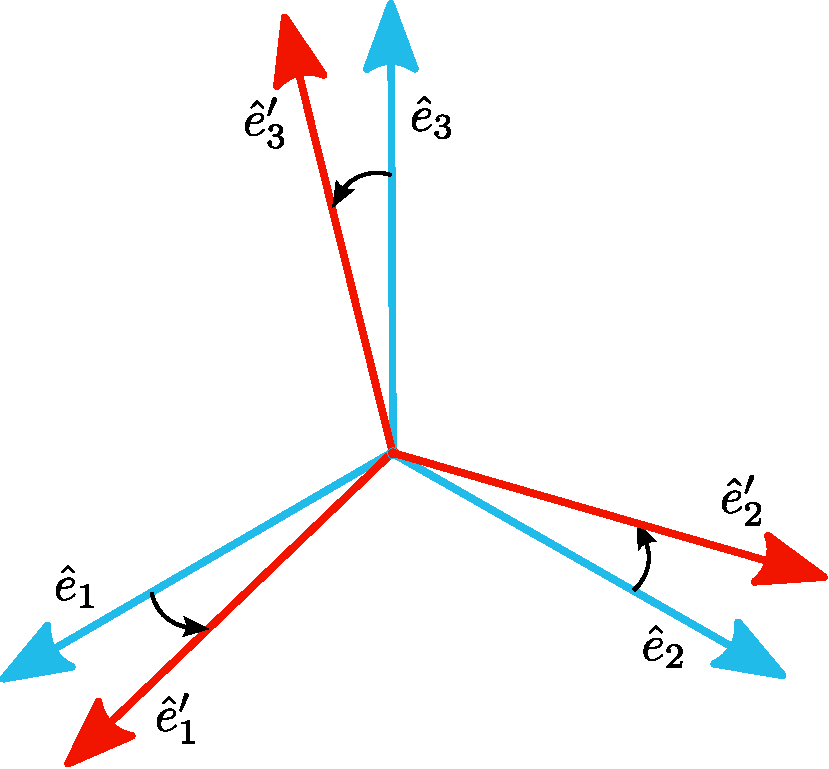
\includegraphics[width=6cm]{Figuras/fig-rotacion-bases.pdf}
    \caption{Una transformación ortogonal de dos bases ortonotmales en 3 dimensiones, $\hat{e}_i$ y $\hat{e}'_j$}
    \label{fig:bases-ortonormales}
\end{figure}

Respecto de esta nueva base, un vector $\vec{v}$ cualquiera puede ser descompuesto en sus componentes $v_i'$ \emph{en la base} $\{ \hat{e}_i'\}_{i=1}^n$,
\begin{equation}
    \vec{v} = \sum_{i=1}^n v_i' \hat{e}'_i \ .
\end{equation}

Dado que, si bien dan origen a sistemas de coordenadas diferentes, ambas bases se encuentran en el mismo espacio vectorial, ¿Cómo podemos relacionar ambas bases entre sí? Para ello, haremos uso de una \textbf{matriz de transformación}, definida como
\begin{equation}
    A = \begin{pmatrix}
        a_{11} & a_{12} & \dots & a_{1n} \\
        a_{21} & a_{22} & \dots & a_{2n} \\
        \vdots & \vdots & \ddots & \vdots \\
        a_{n1} & a_{n2} & \dots & a_{nn}
    \end{pmatrix} =
    \begin{pmatrix}
        \hat{e}_1 \cdot \hat{e}'_1 & \hat{e}_1 \cdot \hat{e}'_2 & \dots & \hat{e}_1 \cdot \hat{e}'_n \\
        \hat{e}_2 \cdot \hat{e}'_1 & \hat{e}_2 \cdot \hat{e}'_2 & \dots & \hat{e}_2 \cdot \hat{e}'_n \\
        \vdots & \vdots & \ddots & \vdots \\
        \hat{e}_n \cdot \hat{e}'_1 & \hat{e}_n \cdot \hat{e}'_2 & \dots & \hat{e}_n \cdot \hat{e}'_n
    \end{pmatrix} \ .
\end{equation}

De este modo, un vector de la base $\vec{e}'_i$ puede escribirse también en términos de la base $\vec{e}_i$,
\begin{equation} \label{eq:transformacion-coordenadas}
    \hat{e}'_i = \sum_{j=1}^n a_{ij} \hat{e}_j \ ,
\end{equation}
por lo que podemos reescribir el vector $\vec{v}$ como
\begin{equation} \label{eq:transformacion-vector}
    \vec{v} = \sum_{i=1}^n v'_i \left( \sum_{j=1}^n a_{ij} \hat{e}_j \right) \ .
\end{equation}

\subsection{Convenio de suma de Einstein}

Antes de continuar la discusión, es útil introducir el  \textbf{convenio de suma de Einstein}, que establece que en toda expresión donde se repitan dos índices iguales, \emph{existe una suma implícita sobre todo el rango de variación del índice}. Es más, el índice de suma \emph{es una etiqueta arbitraria}, por lo que puede ser renombrada a conveniencia.

Por ejemplo, las expresiones \eqref{eq:vector-posicion} y \eqref{eq:transformacion-vector} pueden reescribirse como
\begin{align}
    \vec{v} & = v_i \hat{e}_i \, , \\
    \vec{v} & = v'_i a_{ij} \hat{e}_j .
\end{align}

Además, dado que existe una suma implícita, podemos aplicar la delta de Kronecker para reemplazar índices en una multiplicación, de modo que
\begin{equation}
    a_{ij} b_{jk} \delta_{ki} = a_{ij} b_{ji} = a_{kj} b_{jk} \ .
\end{equation}

\section{Covarianza y contravarianza}

En la sección anterior, vimos que podemos reescribir un vector $\vec{x} = x_i \hat{e}_i$ en términos de una segunda base ortonormal $\{\hat{e}'_i\}_{i=1}^n$ como
\begin{equation} \label{eq:transformacion-vector-einstein}
    \vec{x} = x'_i a_{ij} \hat{e}_j \ .
\end{equation}
Comparando esta expresión con $\x = x_i \hat{e}_i$, observamos que \emph{las componentes de un vector} transforman como
\begin{equation} \label{eq:transformacion-componentes}
    x'_j = a_{ji} x_i \ , 
\end{equation}
donde la inversión de los índices en las componentes de la matriz representa que estamos considerando la matriz transversa.

Nos gustaría poder encontrar una expresión explícita para dicha matriz. Para ello, podemos derivar la expresión \eqref{eq:transformacion-componentes} respecto a las coordenadas $x_i$, obteniendo
\begin{equation}
    a_{ji} = \frac{\partial x'_j}{\partial x_i} \ ,
\end{equation}
mientras que la transformación inversa satisface
\begin{equation}
    a_{ij} = \frac{\partial x_i}{\partial x'_j} \ .
\end{equation}

De este modo, podemos reescribir la ecuación \eqref{eq:transformacion-componentes}, con lo que \emph{las componentes de los vectores transforman, bajo transformaciones ortogonales, como}
\begin{equation}
    x'_i = \frac{\partial x'_i}{\partial x_j} A_j \ .
\end{equation}

Uno podría esperar que todos los vectores transformaran según esta regla. Sin embargo, veamos qué ocurre para el vector gradiente de un campo escalar, $\nabla\phi$, donde $(\nabla \phi)_j = (\partial \phi/\partial x_j )\vec{e}_j$. Tenemos, por regla de la cadena,
\begin{equation}
    (\nabla \phi)'_i = \frac{\partial \phi}{\partial x'_i} = \frac{\partial x_j}{\partial x'_i} \frac{\partial \phi}{\partial x_j} \ ,
\end{equation}
que es \emph{una ley de transformación diferente}. Sin embargo, ambas cantidades corresponden a vectores. ¿Cómo explicamos esta diferencia?

El hecho radica en que, en efecto, ambas cantidades son vectores \emph{en coordenadas cartesianas}, pero no necesariamente \emph{en cualquier sistema de coordenadas}. Por ello, es conveniente introducir las nociones de vectores \textbf{covariantes} y vectores \textbf{contravariantes}. En este curso esta distinción no es necesaria, pero quienes deseen trabajar en gravitación o en altas energías, deberán comenzar a tener en cuenta estas nociones.

\begin{defi} \marginnote{Vector contravariante y vector covariante}
    Un vector $\vec{v}$ es denominado \textbf{contravariante} cuando, al ser sometido a una transformación ortogonal, transforma según la regla
    \begin{equation} \label{eq:contravariante}
        v'_i = \frac{\partial x'_i}{\partial x_j} v_j \ ,
    \end{equation}
    y se denomina \textbf{covariante} cuando transforma según la regla
    \begin{equation} \label{eq:covariante}
        v'_i = \frac{\partial x_j}{\partial x_i'} v_j \ .
    \end{equation}

    Las componentes del vector posición siempre transforman como vectores contravariantes.
\end{defi}


Al trabajar en sistemas no cartesianos, es común representar los vectores contravariantes con superíndices en lugar de subíndices, de modo que las reglas \eqref{eq:contravariante} y \eqref{eq:covariante} se suelen escribir como
\begin{align*}
    v'^i & = \frac{\partial x'^{i}}{\partial x^j} v^j \ , \\
    v'_i & = \frac{\partial x^j}{\partial x'^{i}} v_j \ .
\end{align*}

Al utilizar esta convención, la suma se representa al tener \emph{índices cruzados}, es decir, índices repetidos tanto como superíndice y como subíndice.

\section{Transformaciones Ortogonales}

La discusión hecha hasta ahora es válida para cualquier transformación de coordenadas entre dos bases distintas. Para los efectos de este curso, nos interesa trabajar únicamente con \emph{transformaciones ortogonales}.

\begin{defi} \marginnote{Transformación ortogonal}
    Una \textbf{transformación ortogonal} es aquella transformación de cambio de base que permite convertir una base ortonormal $\{\hat{e}_i\}_{i=1}^n$ en una nueva base ortonormal $\{\hat{e}'_i\}_{i=1}^n$.
\end{defi}

Para asegurarnos que la transformación \eqref{eq:transformacion-coordenadas} sea una transformación ortogonal, debe además satisfacer que
\begin{align}
    \delta_{ij} & = \hat{e}'_i \cdot \hat{e}'_j \\
    & = \left( \sum_{k=1}^n a_{ik} \hat{e}_k \right) \left( \sum_{l=1}^n a_{jl} \hat{e}_l \right) \\
    & = \sum_{k=1}^n \sum_{l=1}^n a_{ik} a_{jl} (\hat{e}_k \cdot \hat{e}_l) \\
    & = \sum_{k=1}^n \sum_{l=1}^n a_{ik} a_{jl} \delta_{kl} \\
    & = \sum_{k=1}^n a_{ik} a_{jk} \ , \label{eq:delta-transformacion-ortogonal}
\end{align}
o bien, matricialmente,
\begin{equation}\label{eq:condicion-matricial}
    A \cdot (A^T) = I \ ,
\end{equation}
que al calcular el determinante, observamos que
\begin{equation}
    \det(A)^2 = 1 \ , 
\end{equation}
de modo que una transformación ortogonal deberá satisfacer que $\det(A) = 1$, caso en que se denomina \emph{transformación propia}, o bien que $\det(A) = -1$, lo que se conoce como \emph{transformación impropia}.

En particular, de \eqref{eq:condicion-matricial} podemos observar que para una transformación ortogonal, $A^T = A^{-1}$, es decir, la transpuesta de la transformación coincide con su inversa, de modo que también se satisface que
\begin{equation}
    (A^T) \cdot A = I \ ,
\end{equation}
o en notación indicial,
\begin{equation}
    \sum_{k=1}^n a_{ki} a_{kj} =  \delta_{ij} \ .
\end{equation}

\section{Tensores Cartesianos}

Hasta ahora, hemos discutido las propiedades de los vectores, elementos con los que ya somos familiares. Sin embargo, seguimos sin responder la incógnita de \emph{¿qué es un tensor?}. Para ello, introduzcamos una operación entre vectores.

\begin{defi}\marginnote{Producto externo}
    Dados dos vectores $\vec{u} = u_i \hat{e}_i$ y $\vec{v} = v_i \hat{e}_i$, se define el \textbf{producto externo} entre ambos vectores como la cantidad
    \begin{equation}
        T_{ij} = u_i v_j \ .
    \end{equation}
\end{defi}

Como podemos ver de la definición anterior, necesitamos de \emph{dos índices} para definir el producto externo. ¿Qué ocurre con esta cantidad si, en lugar de utilizar la base $\hat{e}_i$, utilizamos la base $\hat{e}'_i$? En otras palabras, ¿cómo transforma $T_{ij}$ bajo transformaciones ortogonales? Notamos que
\begin{equation}
    T'_{ij} = u'_i v'_j = (a_{ik}u_k)(a_{jl} v_l) = a_{ik} a_{jl} (u_k v_l) =  a_{ik} a_{jl} T_{kl} \ .
\end{equation}

Observamos pues, que $T_{ij}$ transforma de manera similar a los vectores bajo transformaciones ortogonales. A cantidades que siguen una regla de transformación de este tipo, las llamamos \emph{tensores (cartesianos) de rango 2}, pues requerimos de dos matrices de transformación para definirlas adecuadamente. Observamos que, para un espacio de $n$ dimensiones, estos elementos tendrán $n^2$ componentes.

Esta noción puede ampliarse a más dimensiones, según la siguiente definición,
\begin{defi} \marginnote{Tensor cartesiano}
    Dado un espacio de $n$ dimensiones, el conjunto de $n^r$ cantidades $T_{i_1 i_2 \dots i_r}$ definidas en cada sistema ortogonal de coordenadas, son las componentes de un \textbf{tensor cartesiano de rango} $\mathbf{r}$ si, bajo transformaciones ortogonales, sus valores siguien la regla de transformación
    \begin{equation}
        T'_{i_1 i_2 \dots, i_r} = a_{i_1 j_1} a_{i_2 j_2} \dots a_{i_r j_r} T_{j_1 j_2 \dots j_r} \ . 
    \end{equation}
\end{defi}

Gracias a esta definición, observamos que los \textbf{vectores}, que tienen una sola matriz de transformación en su definición \eqref{eq:transformacion-vector}, son \emph{tensores de rango 1}. A su vez, los \textbf{escalares} son cantidades que no se ven modificadas frente a una transformación de coordendas, de modo que $\rho' = \rho$. Por ello, podemos considerarlos \emph{tensores de rango 0}.

\begin{ejemplo}
    \textbf{Tensor de inercia.}

    Consideremos un cuerpo con densidad $\rho(x_i)$, contenido en una región $V$ que rota \emph{rígidamente} respecto de un eje con dirección $\hat{\omega}$ con velocidad angular $\omega$. Entonces, podemos hallar su momento angular respecto al origen del sistema (ubicado sobre el eje de rotación) como
    \begin{align*}
        \vec{L} & = \int_V \x \times d\vec{p} \\
        & = \int_V \rho(x) \x \times \vec{v} \ dV \\
        & = \int_V \rho(x) \x \times (\vec{\omega} \times \x) \ dV \ .
    \end{align*}
    Usando la identidad $\vec{A} \times (\vec{B} \times \vec{C}) = \vec{B} (\vec{A} \cdot \vec{C}) - \vec{C} (\vec{A} \cdot \vec{B})$, podemos escribir
    \begin{equation*}
        \vec{L} = \int_V \rho(x) [\vec{\omega}(\x \cdot \x) - \x (\vec{\omega} \cdot \x)] \ dV \ ,
    \end{equation*}
    o en términos de las componentes del vector,
    \begin{align*}
        L_i & = \int_V \rho(x) [\omega_i(x_k x_k) - x_i(\omega_j x_j)] \ dV \\
        & = \int_V \rho(x) [(\delta_{ij} \omega_j)(x_k x_k) - x_i(\omega_j x_j)] \ dV \\
        & = \left( \int_V \rho(x) [\delta_{ij} (x_k x_k) - x_i x_j] \ dV \right) \omega_j \ ,
    \end{align*}
    es decir, 
    \begin{equation*}
        L_i = I_{ij} \omega_j \, 
    \end{equation*}
    donde $I_{ij}$ es el \emph{tensor de inercia} definido como
    \begin{equation*}
        \int_V \rho(x) [\delta_{ij} (x_k x_k) - x_i x_j] \ dV \ .
    \end{equation*}

    ¿Es esta cantidad efectivamente un tensor cartesiano? Revisemos cómo transforma bajo una transformación ortogonal,
    \begin{align*}
        I'_{ij} & = \int_V \rho'(x') [\delta_{ij} (x'_k x'_k) - x'_i x'_j] \ dV' \\
        & = \int_V \underbrace{\rho(x)}_{\text{Escalar}} [\delta_{ij}\underbrace{(x_k x_k)}_\text{Escalar} - (a_{il} x_l)(a_{jm} x_m)] \ dV \\
        & = \int_V \rho(x) [(a_{il}a_{jl})(x_k x_k) - (a_{il} x_l)(a_{jm} x_m)] \ dV \\
        & = \int_V \rho(x) [(a_{il}a_{jm}\delta_{lm})(x_k x_k) - (a_{il} x_l)(a_{jm} x_m)] \ dV \\
        & = (a_{il} a_{jm}) \int_V \rho(x) [(\delta_{lm})(x_k x_k) - x_l x_m] \ dV \\
        & = a_{il} a_{jm} I_{lm} \ ,
    \end{align*}
    de modo que efectivamente $I_{jl}$ transforma como un tensor cartesiano.
\end{ejemplo}

\subsection{Propiedades}

En este contexto, vale la pena mencionar con algo más de detalle a dos propiedades.

\begin{propiedad}
    \textbf{Propiedades de los tensores cartesianos.}

    \begin{enumerate}
        \item Si \emph{todas las componentes de un tensor se anulan en un sistema coordenado ortogonal}, ellas se anularán \emph{en todo sistema coordenado ortogonal}.  Esta propiedad nos interesa, ya que nos indica que la anulación de un tensor \textbf{es una propiedad intrínseca} de este. De esta propiedad surge la importancia de utilizar tensores en Física, pues nos permite plantear leyes \emph{que no dependen del sistema coordenado en que trabajamos}, sino únicamente del fenómeno estudiado.
        
        Por ejemplo, podemos estar estudiando el momento de inercia de un cuerpo en movimiento, el cual es un tensor de rango 2. Si diera la casualidad de que este es cero en algún sistema coordenado ortogonal, esto quiere decir que, \textbf{en cualquier sistema coordenado ortogonal}, el cuerpo \emph{no se encuentra rotando}.
    
        \item Existen algunos \textbf{tensores invariantes} o \textbf{isotrópicos}, los cuales tienen siempre las mismas componentes \emph{en cualquier sistema coordenado}. Un ejemplo de estos es la delta de Kronecker, pues en cualquier sistema coordenado tendrá las mismas componentes, 1 si $i=j$ y 0 si $i\neq j$.
        
        En efecto, podemos observar que la delta de Kronecker transforma como
        \begin{equation}
            \delta'_{ij} = a_{ik} a_{jl} \delta_{kl} = a_{ik} a_{jk} = \delta_{ij} \ .
        \end{equation}
    \end{enumerate}
\end{propiedad}



\section{Álgebra Tensorial}

Dicho rápido y sencillo, hemos visto que los tensores de rango 1 y rango 2 se comportan como vectores columna y como matrices, respectivamente. Por ello, esperaríamos que sea posible definir operaciones tensoriales similares a las definidas para estos elementos, incluyendo la posibilidad de construir tensores a partir de otros.

\begin{itemize}
    \item \textbf{Adición y sustracción.} Se define la adición (o suma) y sustracción (o resta) de dos tensores \emph{del mismo orden} componente a componente, es decir,
    \begin{align}
        S_{ij \dots k} & = V_{ij \dots k} + W_{ij \dots k} \ , \\
        D_{ij \dots k} & = V_{ij \dots k} - W_{ij \dots k} \ .
    \end{align}
    % \item \textbf{Producto por escalar.}
    \item \textbf{Permutación de índices.} La operación de permutar dos índices de un tensor de rango $r$, define un nuevo tensor de rango $r$. Es decir, dado un tensor $T_{ijk \dots l}$ de rango $r$, la cantidad
    \begin{equation}
        B_{ijk \dots l} = T_{ikj \dots l} 
    \end{equation}
    es también un tensor de rango $r$.

    \item \textbf{Producto tensorial, o directo.} De manera similar al \emph{producto externo} de dos vectores que calculamos anteriormente, podemos definir el producto entre dos tensores de diferente rango, digamos $r$ y $s$, lo que permite formar un nuevo vector de rango $r+s$,
    \begin{equation}
        C_{i_1 i_2 \dots i_{r+s}} = A_{i_1 i_2 \dots i_r} \cdot B_{i_{r+1} i_{r+2} \dots i_{r+s}} \ .
    \end{equation}
    
    En este caso, es relevante respetar la posición de los índices en el producto, pues en general el tensor $C_{ij} = A_i B_j$ será distinto al vector $D_{ij} = A_j B_i$, como consecuencia de la permutación de índices.

    Esta operación incluye, por supuesto, el producto entre un tensor de rango 0 (un escalar) y un tensor de rango $r$, definiendo el \emph{prodcuto por un escalar}.

    \item \textbf{Contracción de índices.} El producto escalar entre dos vectores nos entrega un escalar en lugar de un tensor de orden 2, como consecuencia de la repetición de índices en el producto. De manera similar, la repetición de dos índices dentro de un tensor de orden $r$ (digamos, el $s$-ésimo y el $t$-ésimo índice), es equivalente a un tensor de orden $r-2$,
    \begin{equation}
        B_{i_1 i_2 \dots i_{r-2}} = A_{i_1 i_2 \dots j \dots j \dots i_{r-2}} \ ,
    \end{equation}
    o de forma equivalente,
    \begin{equation}
        B_{i_1 i_2 \dots} = A_{i_1 i_2 \dots i_r} \delta_{i_s i_t} \ .
    \end{equation}

    \item \textbf{Ley del cociente.} Consideremos el caso en que tenemos una expresión de la forma
    \begin{equation}\label{eq:ley-cociente}
        A_{pq \dots k \dots m} B_{ij \dots k \dots n} = C_{pq \dots m ij \dots n} \ ,
    \end{equation}
    donde sabemos que $B$ y $C$ son tensores de rango $r$ y $s$, respectivamente, pero desconocemos si $A$ es un tensor. La ley del cociente establece que \emph{si la relación \eqref{eq:ley-cociente} es válida en cualquier sistema de coordenadas, entonces} $A$ es un tensor de orden $s-r+2$. La demostración (para el caso $r=s=2$) puede ser hallada en el capítulo 26, sección 7 de Riley \cite{Riley}.
    
    \item \textbf{Simetría.} Cuando un tensor no cambia bajo la permutación de dos de sus índices, 
    \begin{equation}
        T_{i_1 i_2 \dots i_s \dots i_t \dots i_r} = T_{i_1 i_2 \dots i_t \dots i_s \dots i_r} \ , 
    \end{equation}
    se dice que este es \emph{simétrico} respecto a dichos índices. Si, en cambio,
    \begin{equation}
        T_{i_1 i_2 \dots i_s \dots i_t \dots i_r} = - T_{i_1 i_2 \dots i_t \dots i_s \dots i_r} \ ,
    \end{equation}
    decimos que el tensor es \emph{antisimétrico} respecto de dichos índices. En general, un tensor de rango $r$ puede escribirse como la suma de un tensor simétrico y un tensor antisimétrico respecto de la misma permutación de índices, de modo que
    \begin{align}
        T_{i_1 i_2 \dots i_s \dots i_t \dots i_r} & = \frac{1}{2} (T_{i_1 i_2 \dots i_s \dots i_t \dots i_r} + T_{i_1 i_2 \dots i_t \dots i_s \dots i_r}) + \frac{1}{2}(T_{i_1 i_2 \dots i_s \dots i_t \dots i_r} - T_{i_1 i_2 \dots i_t \dots i_s \dots i_r}) \\
        & = S_{i_1 i_2 \dots i_s \dots i_t \dots i_r} + A_{i_1 i_2 \dots i_s \dots i_t \dots i_r} \ .
    \end{align}

    En física, a veces es común utilizar la siguiente notación,
    \begin{align}
        T_{i_1 i_2 \dots (i_s| \dots |i_t) \dots i_r} & \equiv S_{i_1 i_2 \dots i_s \dots i_t \dots i_r} \ , \\
        T_{i_1 i_2 \dots [i_s| \dots |i_t] \dots i_r} & \equiv A_{i_1 i_2 \dots i_s \dots i_t \dots i_r} \ ,
    \end{align}
    donde los índices entre paréntesis o corchetes son los índices respecto de los cuales el tensor es simétrico o antisimétrico.

    Un tensor \textbf{completamente simétrico} de rango $r$ es aquel que es simétrico respecto a la permutación de cada par de índices. Este tendrá $\frac{(n+r-1)!}{(n-1)! r!}$ componentes linealmente independientes.

    De forma análoga, un tensor \textbf{completamente antisimétrico} de rango $r$ es aquel que es antisimétrico respecto a la permutación de cada par de índices. Este tendrá $\frac{n!}{(n-r)! r!}$ componentes linealmente independientes. En particular, un tensor de rango $r=n$, tendrá \emph{una única componente linealmente independiente}.
\end{itemize}

\section{Pseudovectores y pseudotensores}

Hasta ahora, de manera implícita, hemos utilizado transformaciones ortogonales \emph{propias}, es decir, que solo rotan el sistema, pero no modeifican la orientación de los tensores. Sin embargo, al considerar transformaciones \emph{impropias}, que no solo rotan el sistema sino que realizan una inversión de coordenadas o \emph{reflexión} ($x_i \to -x_i$). Cuando también incluimos este tipo de transformaciones, los vectores siguen cumpliendo la regla de transformación \eqref{eq:transformacion-vector}. Sin embargo, existen ciertas cantidades físicas que comúnmente supondríamos como vectores, que \textbf{no transforman de igual manera} bajo una reflexión, como es el caso de aquellas relacionadas a cantidades \emph{angulares}, como la velociadad angular, el torque o el momento angular.

\begin{defi} \marginnote{Pseudovector}
    Las cantidades que transforman según la regla
    \begin{equation} \label{eq:pseudovector}
        \vec{v}' = \det(A) A \, \vec{v} \ ,
    \end{equation}
    se denominan \textbf{pseudovectores}, o \textbf{vectores axiales}.
\end{defi}

De forma análoga, es posible extender esta noción a tensores y \emph{pseudotensores}.

\begin{defi} \marginnote{Pseudotensor}
    Los elementos que transforman según la regla
    \begin{equation}
        T'_{i_1 i_2 \dots i_r} = \det(A) a_{i_1 j_1} a_{i_2 j_2} \dots a_{i_n j_n} T_{j_1 j_2 \dots j_r} 
    \end{equation}
    se denominan \textbf{pseudotensores}.
\end{defi}

\subsection{Propiedades}

\begin{propiedad}
    \textbf{Propiedades de los pseudotensores.}

    \begin{enumerate}
        \item La suma y la diferencia de dos pseudotensores del mismo rango es también un pseudotensor del mismo rango.
        \item El producto tensorial de dos pseudotensores es un tensor cartesiano.
        \item El producto tensorial de un pseudotensor y un tensor es un pseudotensor.
        \item La contracción de dos índices de un pseudotensor define un nuevo pseudotensor.
        \item Un \textbf{pseudoescalar} es una cantidad que cambia de signo bajo una transformación impropia.
        \item En física, es común considerar únicamente transformaciones propias. En estos casos, la distinción entre tensores y pseudotensores no es necesaria.
    \end{enumerate}
\end{propiedad}

\subsection{Símbolo de Levi-Civita}

\begin{defi} \textbf{Símbolo de Levi-Civita}
    En un espacio $n-$dimensional, se define el \textbf{símbolo de Levi-Civita} como un objeto de $n$ índices \emph{totalmente antisimétrico}, es decir,
    \begin{equation}
        \varepsilon_{ijkl\dots} = -\varepsilon_{jikl\dots} = - \varepsilon_{kjil\dots} = - \varepsilon_{ljki} = \varepsilon_{jilk} = \dots \ ,
    \end{equation}
    tal que en todo sistema de coordenadas,
    \begin{equation}
        \varepsilon_{123 \dots n} = 1 \ .
    \end{equation}

    De forma equivalente, se puede definir como
    \begin{equation}
        \varepsilon_{i_1 \dots i_n} = \begin{dcases}
            1, \qquad \text{si } i_1 \dots i_n \text{ es una permutación par de } 12 \dots n \ , \\
            -1, \quad \text{si } i_1 \dots i_n \text{ es una permutación impar de } 12 \dots n \ , \\
            0, \qquad \text{en otro caso} \ .
        \end{dcases}
    \end{equation}
\end{defi}

% \subsubsection*{Propiedades}

\begin{propiedad}
    \textbf{Propiedades del símbolo de Levi-Civita.}

    \begin{enumerate}
        \item El símbolo de Levi-Civita puede utilizarse para calcular determinantes, mediante la relación
        \begin{equation}
            det(A) = a_{1 j_1} a_{2 j_2} \dots a_{n j_n} \varepsilon_{j_1 j_2 \dots j_n} \ .
        \end{equation}

        \item El símbolo de Levi-Civita transforma como un pseudotensor.
        
        De la propiedad 1, se desprende que el símbolo de Levi-Civita transforma, bajo una transformación arbitraria, como
        \begin{equation}
            \varepsilon'_{i_1 \dots i_n} = \frac{1}{\det(A)} a_{i_1 j_1} a_{i_2 j_2} \dots a_{i_n j_n} \varepsilon_{j_1 j_2 \dots j_n} \ .
        \end{equation}
        Como en las transformaciones ortogonales, $\det(A) = 1/\det(A) = \pm 1$, concluímos que el símbolo de Levi-Civita \emph{transforma como un pseudotensor}.

        \item El símbolo de Levi-Civita puede ser utilizado para representar productos vectoriales entre dos vectores en notación tensorial, de modo que si $\vec{C} = \vec{A} \, \times \, \vec{B}$, podemos escribir
        \begin{equation}
            C_i = \varepsilon_{ijk} A_j B_k \ .
        \end{equation}
        Como consecuencia, \emph{todo vector que se obtiene a partir del producto vectorial entre dos vectores, es un pseudovector}, lo que explica por qué las cantidades angulares se comportan como pseudovectores.

        \item El símbolo de Levi-Civita satisface la identidad
        \begin{equation}
            \varepsilon_{i_1 \dots i_n} = \left| \begin{array}{cccc}
                \delta_{i_1 1} & \delta_{i_1 2} & \dots & \delta_{i_1 n} \\
                \delta_{i_2 1} & \delta_{i_2 2} & \dots & \delta_{i_2 n} \\
                \vdots & \vdots & \ddots & \vdots \\
                \delta_{i_n 1} & \delta_{i_n 2} & \dots & \delta_{i_n n} 
            \end{array} \right| \ ,
        \end{equation}
        de donde es directo hallar que el producto de dos símbolos de Levi-Civita se puede hallar como
    \begin{equation}
        \varepsilon_{i_1 i_2 \dots i_n} \varepsilon_{j_1 j_2 \dots j_n} = \left| \begin{array}{cccc}
            \delta_{i_1 j_1} & \delta_{i_1 j_2} & \dots & \delta_{i_1 j_n} \\
            \delta_{i_2 j_1} & \delta_{i_2 j_2} & \dots & \delta_{i_2 j_n} \\
            \vdots & \vdots & \ddots & \vdots \\
            \delta_{i_n j_1} & \delta_{i_n j_2} & \dots & \delta_{i_n j_n} \\
        \end{array}
        \right| \ .
    \end{equation}

    \item En tres dimensiones, el símbolo de Levi-Civita satisface las identidades
    \begin{align}
        \varepsilon_{ijk} \varepsilon_{lmk} & = \delta_{il} \delta_{jm} - \delta_{im} \delta_{jl} \ , \\
        \varepsilon_{ijk} \varepsilon_{ljk} & = 2 \delta_{il} \ , \\
        \varepsilon_{ijk} \varepsilon_{ijk} & = 6 \ .
    \end{align}
    
    \end{enumerate}
\end{propiedad}

\subsection{Tensores duales}

A cualquier (pseudo-)tensor totalmente antisimétrico de rango $r$ en $n$ dimensiones se le puede asociar un (pseudo-)tensor totalmente antisimétrico de rango $(n-r)$, pues ambos tienen el mismo número de componentes linealmente independientes.

\begin{defi} \marginnote{Pseudotensor dual}
    Si $A_{i_1 \dots i_r}$ es un tensor totalmente antisimétrico de rango $r$, se define un \textbf{pseudotensor dual} de rango $n-r$ como
    \begin{equation}
        \mathcal{A}_{i_1 \dots i_{n-r}} = \frac{1}{r!} \varepsilon_{i_1 \dots i_{n-r} j_1 \dots j_r} A_{j_1 \dots j_r} \ ,
    \end{equation}
    mientras que la transformación inversa se define como
    \begin{equation}
        A_{i_1 \dots i_{r}} = \frac{1}{(n-r)!} \varepsilon_{i_1 \dots i_{r} j_1 \dots j_{n-r}} \mathcal{A}_{j_1 \dots j_{n-r}} \ .
    \end{equation}
\end{defi}

Cuando trabajamos en tres dimensiones, a cualquier tensor de rango 3 totalmente antisimétrico, $A_{ijk}$, le podemos asociar un pseudoescalar dual $\mathcal{A}$, tal que
\begin{equation}
    \mathcal{A} = \frac{1}{3!} \varepsilon_{ijk} A_{ijk} \ , \qquad A_{ijk} = \varepsilon_{ijk} \mathcal{A} \ ,
\end{equation}
y a cualquier tensor antisimétrico $A_{ij}$ se le puede asociar un pseudovector $\mathcal{A}_i$, tal que
\begin{equation}
    \mathcal{A}_i = \frac{1}{2} \varepsilon_{ijk} A_{jk} \ , \qquad A_{ij} = \varepsilon_{ijk} \mathcal{A}_k \ ,
\end{equation}
y viceversa.

En Física, el uso de tensores y sus duales nos permite tener cantidades diferentes que contienen la misma información, y que pueden ser útiles en diferentes contextos. Por ejemplo, el \emph{momento multipolar magnético de orden 1}, $M_{ij} = - M_{ji}$, contiene la misma información que el pseudovector \emph{momento magnético}, definido como $\mu_i = \varepsilon_{ijk} M_{jk}/2$.

\section{Análisis tensorial}

En el curso de Física Matemática I, ya estudiaron la noción de \emph{análisis vectorial}, que correspondía al uso del operador nabla en diferentes sistemas coordenados. En este, hicieron uso de las nociones de \emph{campo escalar} y \emph{campo vectorial}. Estas nociones pueden también extenderse a elementos de mayor rango mediante los campos tensoriales.
\begin{defi} \marginnote{Campo tensorial}
    Se define un \textbf{campo tensorial} como la función que asocia a cada punto del espacio con un tensor $T_{i_1 i_2 \dots i_r}$, es decir,
    \begin{equation}
        x \mapsto T_{i_1 i_2 \dots i_r}(x) \ .
    \end{equation}
\end{defi}

\subsection{Derivación}

Dado que un campo tensorial de rango $r$ consta de $n^r$ cantidades definidas en cada punto del espacio, podemos derivar cada una de estas cantidades respecto a las $n$ coordenadas del espacio, obteniendo $n^{r+1}$ derivadas parciales
\begin{equation}
    \frac{\partial T_{i_1 \dots i_r}}{\partial x_j} \equiv \partial_j T_{i_1 \dots i_r} \ ,
\end{equation}
que forman un tensor cartesiano de rango $r+1$ bajo transformaciones ortogonales. En efecto,
\begin{align}
    (\partial_j T_{i_1 \dots i_r})' & = \frac{\partial T'_{i_1 \dots i_r}}{\partial x'_j} \\
    & = \frac{\partial}{\partial x'_j}(a_{i_1 j_1} \dots a_{i_r j_r} T_{j_1 \dots j_r}) \\
    & = a_{i_1 j_1} \dots a_{i_r j_r} \frac{\partial T_{j_1 \dots j_r}}{\partial x'_j} \ .
\end{align}
Usando ahora la regla de la cadena, tenemos que
\begin{equation}
    \frac{\partial T_{j_1 \dots j_r}(x')}{\partial x'_j} = \frac{\partial T_{j_1 \dots j_r}(x')}{\partial x_k} \frac{\partial x_k}{\partial x'_j} = a_{jk} \frac{\partial T_{j_1 \dots j_r}(x')}{\partial x_k}\ ,
\end{equation}
de modo que
\begin{align}
    (\partial_j T_{i_1 \dots i_r})' & = a_{i_1 j_1} \dots a_{i_r j_r} \frac{\partial T_{j_1 \dots j_r}(x')}{\partial x_k} \frac{\partial x_k}{\partial x'_j} \\
    & = a_{i_1 j_1} \dots a_{i_r j_r}  a_{jk} \frac{\partial T_{j_1 \dots j_r}(x')}{\partial x_k} \\
    & = a_{i_1 j_1} \dots a_{i_r j_r}  a_{jk} (\partial_k T_{j_1 \dots j_r}) \ ,
\end{align}
comprobando así que transforma como un tensor de orden $r+1$.

También podemos calcular la derivada de un tensor de rango $r$ respecto de un parámetro $t$ \emph{independiente de las coordenadas}. En este caso, el resultado es también un tensor de orden $r$,
\begin{equation}
    \frac{d T'_{i_1 \dots i_r}}{dt} = a_{i_1 j_1} \dots a_{i_r j_r} \frac{dA_{j_1 \dots j_r}}{dt} \ . 
\end{equation}

De una manera similar, podemos operar sobre este nuevo tensor \emph{derivada} con todas las operaciones tensoriales disponibles. En particular, podemos definir el operador nabla en un espacio de $n$ dimensiones. En notación indicial, dado un campo escalar $\phi$ y un vector $\vec{A}$, tenemos
\begin{align}
    (\nabla \phi)_i & = \partial_i \phi \ , \\
    \nabla \cdot \vec{A} & = \partial_i A_i \ , \\
    (\nabla \times \vec{A})_i & = \varepsilon_{ijk} \partial_j A_k \ , \\
    \nabla^2 \phi & = \partial_i \partial_i \phi \ .
\end{align}

\subsection{Integración}

Al igual que tenemos \emph{integrales vectoriales} para campos vectoriales, que puedn dar como resultado un vector o un escalar, podemos definir \emph{integrales tensoriales} para campos tensoriales. En particular, revisaremos las integrales de línea, superficie y volumen.

\subsubsection*{Integrales de línea}

Una integral de línea sobre un campo tensorial $T_{i_i \dots i_r}(x)$ de rango $r$ a lo largo de una curva $\mathcal{C}$ definida por un parámetro $\lambda$ tal que $\lambda_1 < \lambda < \lambda_2$, genera una tensor de rango $r+1$ definido como
\begin{equation}
    C_{j i_1 \dots i_r} = \int_{\mathcal{C}} T_{i_1 \dots i_r} (x) dx_j \ ,
\end{equation}
o de forma explícita,
\begin{equation}
    C_{j i_1 \dots i_r} =  \int_{\lambda_1}^{\lambda_2} T_{i_1 \dots i_r}(x(\lambda)) \left(\frac{dx_j}{d\lambda}(\lambda) \right) d\lambda \ .
\end{equation}

En efecto, observamos que
\begin{align}
    C'_{j i_1 \dots i_r} & = \int_{\lambda_1}^{\lambda_2} [T'_{i_1 \dots i_r}(x(\lambda))] \left[ \frac{dx'_j}{d\lambda}(x) \right] d\lambda \ , \\
    & = \int_{\lambda_1}^{\lambda_2} [a_{i_1 j_1} \dots a_{i_r j_r} T_{j_1 \dots j_r}(x(\lambda))] \left[ \frac{d(a_{jk}x_k)}{d\lambda}(x) \right] d\lambda \ , \\
    & = a_{jk} a_{i_1 j_1} \dots a_{i_r j_r} \int_{\lambda_1}^{\lambda_2} T_{j_1 \dots j_r}(x(\lambda)) \frac{dx_k}{d\lambda}(\lambda) d\lambda \ , \\
    & = a_{jk} a_{i_1 j_1} \dots a_{i_r j_r} C_{k j_1 \dots j_r} \ .
\end{align}

\subsubsection*{Integrales de superficie}

Dado un (pseudo)vector $n_i(x)$ unitario y normal a la superficie $S$ en el punto $x_i$, podemos definir la integral de superficie de un campo tensorial $T_{i_i \dots i_r}(x)$ de rango $r$, que será un (pseudo)tensor de rango $r+1$, como
\begin{equation}
    C_{j i_1 \dots i_r} = \int_S T_{i_1 \dots i_r} (x) dS_j \ , \qquad dS_j = n_j dS \ ,
\end{equation}
donde $dS$ es el elemento de superficie que, por definición, es un escalar.

Comprobamos que esta integral es un tensor, ya que
\begin{align}
    C'_{j i_1 \dots i_r} & = \int_S T'_{i_1 \dots i_r}(x) n'_j dS' \ , \\
    & = \int_S [a_{i_1 j_1} \dots a_{i_r j_r} T_{j_1 \dots j_r}(x)](a_{jk} n_k) dS \ , \\
    & = a_{jk} a_{i_1 j_1} \dots a_{i_r j_r} \int_S T_{j_1 \dots j_r}(x) n_k dS \ , \\
    & = a_{jk} a_{i_1 j_1} \dots a_{i_r j_r} C_{k j_1 \dots j_r} \ .
\end{align}

\subsubsection*{Integrales de volumen}

En este caso, dado un volumen $n-$dimensional, la integral de volumen de un campo tensorial $T_{i_i \dots i_r}(x)$ de rango $r$, es también un tensor de rango $r$, definido como
\begin{equation}
    C_{i_1 \dots i_r} = \int_V T_{i_1 \dots i_r}(x) d^n x \ .
\end{equation}

Efectivamente, observamos que
\begin{align}
    C'_{i_1 \dots i_r} & = \int_V T'_{i_1 \dots i_r}(x) d^n x' \ , \\
    & = \int_V [a_{i_1 j_1} \dots a_{i_r j_r} T_{j_1 \dots j_r}(x)] \left| \frac{\partial x'}{\partial x} \right| d^n x \ , \\
    & = a_{i_1 j_1} \dots a_{i_r j_r} \int_V T_{j_1 \dots j_r}(x) \det(A) d^n x \ , \qquad \det(A) = 1 \\
    & = a_{i_1 j_1} \dots a_{i_r j_r} \int_V T_{j_1 \dots j_r}(x) d^n x \ , \\
    & = a_{i_1 j_1} \dots a_{i_r j_r} C_{j_1 \dots j_r} \ .
\end{align}

\subsubsection*{Teoremas integrales}

El \textbf{teorema fundamental del cálculo} en varias variables puede ser escrito en notación tensorial como
\begin{equation}
    \int_{C_{[A,B]}} (\partial_k T_{i_1 \dots i_r}) dx_k = T_{i_1 \dots i_r}(B) - T_{i_1 \dots i_r}(A) \ ,
\end{equation}
donde $C_{[A,B]}$ es una curva que une los puntos $A$ y $B$.

El \textbf{teorema de Gauss} en 3 dimensiones puede escribirse como
\begin{equation}
    \int_V \partial_j T_{i_1 \dots k \dots i_r}(x) dV = \oint_{\partial V} T_{i_1 \dots k \dots i_r} (x) dS_j \ ,
\end{equation}
y puede generalizarse al caso en el que no necesariamente exista una contracción de índices (no necesariamente hay una divergencia) como
\begin{equation}
    \int_V \partial_j T_{i_1 \dots i_r}(x) dV = \oint_{\partial V} T_{i_1 \dots i_r} (x) dS_j \ .
\end{equation}

El \textbf{teorema de Stokes} se puede escribir de una manera similar, escribiendo los casos donde hay contracción de índices,
\begin{equation}
    \int_S \varepsilon_{ijk} \partial_j T_{i_1 \dots k \dots i_r} dS_i = \oint_{\partial S} T_{i_1 \dots k \dots i_r} dx_k \ ,
\end{equation}
y el caso en que no necesariamente exista una contracción,
\begin{equation}
    \int_S \varepsilon_{ijk} \partial_j T_{i_1 \dots i_r} dS_i = \oint_{\partial S} T_{i_1 \dots i_r} dx_k \ .
\end{equation}


\appendix

% \chapter{Un breve repaso: Espacios vectoriales y espacio de funciones}

\section{Definiciones}

\begin{defi}
    Un \emph{espacio vectorial} sobre un cuerpo $\mathbb{K}$ es una terna $(V, +, \cdot)$ formada por un \textbf{conjunto no vacío} $V$, una \textbf{operación de suma} $+: V \times V \to V$ y una \textbf{operación de producto escalar} $\cdot: \mathbb{K} \times V \to V$, que satisface ocho propiedades: 

    \begin{multicols}{2}   
        \begin{itemize}
            \item[\textbf{EV1}] (Asociatividad) $\vec{x} + (\vec{y} + \vec{z}) = (\vec{x} + \vec{y}) + \vec{z}$. 
            \item[\textbf{EV2}] (Elemento neutro) $\vec{x} + \vec{0} = \vec{0} + \vec{x} = \vec{x}$.
            \item[\textbf{EV3}] (Elemento opuesto) $\vec{x} + (-\vec{x}) = \vec{0}$.
            \item[\textbf{EV4}] (Conmutatividad) $\vec{x} + \vec{y} = \vec{y} + \vec{x}$. 
            \item[\textbf{EV5}] $a(b\vec{x}) = (ab) \vec{x}$.
            \item[\textbf{EV6}] (Distributividad) $a(\vec{x} + \vec{y}) = a \vec{x} + a\vec{y}$.
            \item[\textbf{EV7}] (Distributividad) $(a+b) \vec{x} = a\vec{x} + b\vec{x}$.
            \item[\textbf{EV8}] $1\vec{x} = \vec{x}$.    
        \end{itemize}
    \end{multicols}
\end{defi}

% \begin{defi}
Denotemos por $\mathscr{C}_0 [a,b]$ al conjunto de funciones complejas continuas de una variable real $t \in [a,b]$.
% \end{defi}

Notemos que claramente se cumple:
\begin{shaded}
$$f,g \in \mathscr{C}_0[a,b] ~\Rightarrow~ f + g \in \mathscr{C}_0 [a,b]$$
\end{shaded}

y 
\begin{shaded}
$$f \in \mathscr{C}_0[a,b] ~\mbox{y}~ \lambda \in \mathbb{C} ~\Rightarrow~ \lambda f \in  \mathscr{C}_0[a,b].$$ 
\end{shaded}

\begin{defi}
Una función $f: [a,b] \longrightarrow \mathbb{C}$ es \textbf{seccionalmente continua} si $[a,b]$ tiene una partición finita $a = t_0 < t_1 < \cdots < t_n = b$ tal que $f$ es continua y acotada en cada intervalo abierto $(t_i, t_{i+1}), i = 0, \dots, n-1$.

Denotaremos por $\mathscr{C}[a,b]$ al conjunto de las funciones complejas seccionalmente continuas.
\end{defi}

Geométricamente, $f: [a,b] \longrightarrow \mathbb{C}$ es una curva en el plano complejo y la condición de seccionalmente continua se puede apreciar en la figura \ref{fig:FunciónSC}. 

\begin{figure}
    \centering
    \includegraphics[scale=0.45]{Figuras/FuncionSC.pdf}
    \caption{En (a) una función de la forma $f: [a,b] \rightarrow \mathbb{R}$ y en (b) una función de la forma $f: [a,b] \rightarrow \mathbb{C}$, ambas seccionalmente continuas.}
    \label{fig:FunciónSC}
\end{figure}

Podemos afirmar que los conjuntos $\mathscr{C}_0 [a,b]$ y $\mathscr{C}[a,b]$ forman espacios vectoriales sobre el cuerpo de los complejos. Además, $\mathscr{C}_0 [a,b] \subset \mathscr{C} [a,b].$

\begin{defi}
Consideremos dos funciones $f,g \in \mathscr{C}[a,b]$. Definimos su \textbf{producto escalar}\footnote{Aquí utilizaremos la notación comúnmente utilizada en matemática para el producto escalar, donde el segundo término del producto es el que se conjuga, en este caso, $g$. Comúnmente en física, al usar notación de Dirac, se utiliza que el elemento conjugado es el primero, en este caso, $f$.} como
$$\boxed{\langle f , g \rangle = \int_a^b f(t) g^\ast(t) \,dt }$$
\end{defi}

\begin{propo}[Propiedades del producto escalar] \label{ProductoEscalar}
 Sean $f,g,h \in \mathscr{C}[a,b]$ y  $\lambda \in \mathbb{C}$.
 
 \begin{itemize}
     \item $\langle f , g \rangle = \langle g, f \rangle^*$
     \item $\langle f , g + h \rangle = \langle f , g \rangle + \langle f , h \rangle$
     \item $\langle f + g , h \rangle = \langle f , h \rangle + \langle g , h \rangle$
     \item $\langle \lambda f , g \rangle = \lambda \langle f , g \rangle$
     \item $\langle  f , \lambda g \rangle = \lambda^*\langle f , g \rangle$
     \item Si $f \not\equiv 0$, entonces $\langle f , f \rangle > 0$
 \end{itemize}
\end{propo}


%% Considero que lo comentado es solo una formalidad matemática, que no es relevante al nivel de este curso

% \textbf{Observación:} Con respecto a la última propiedad, se tiene que 
% $$\langle f , f \rangle = \int_a^b |f(t)|^2 \,dt = 0 \color{red}{\nRightarrow} f = 0.$$

% Por esto se define la relación de equivalencia \footnote{$m(E) = 0$ denota que $E$ es un conjunto de medida cero.}
% $$f = g ~ c.t.p ~\Leftrightarrow~ f(t) = g(t), \forall t \in [a,b]-E, \mbox{con}~ m(E) = 0.$$

% Esta relación se expresa diciendo que $f = g $ casi en todas partes.

% \textbf{Notación:} $f \equiv g ~\Leftrightarrow~ f = g ~c.t.p$

% Esencialmente una relación de equivalencia es una relación de igualdad, bajo la cual dos funciones equivalentes se consideran ``iguales". Así, toda función $f = 0 ~c.t.p$, o simplemente $f\equiv 0$, se considera como la función nula.

% \begin{defi}
% Un espacio vectorial complejo dotado de un producto escalar con las propiedades de la proposición \ref{ProductoEscalar}, se conoce como \textbf{espacio pre-Hilbert}.
% \end{defi} 

\begin{defi}
Sea $f \in \mathscr{C}[a,b]$. Definimos su \textbf{norma} como
$$\norm{f} = \sqrt{\langle f,f \rangle} \in \mathbb{R}.$$
\end{defi}

\begin{propo}
Sean $f,g \in \mathscr{C}[a,b]$ y $\lambda \in \mathbb{C}$.

\begin{itemize}
    \item $\norm{f} \geq 0$
    \item $\norm{\lambda f} = |\lambda| \norm{f}$
    \item $|\langle f| g \rangle | \leq \norm{f} \cdot \norm{g}$ (Desigualdad de Cauchy-Schwarz)
    \item $\norm{f \pm g} \leq \norm{f} + \norm{g}$ (Desigualdad triangular)
    \item Si $f \not\equiv 0$, entonces $\norm{f} > 0$.
\end{itemize}
\end{propo}

\begin{demo}
Demostraremos solo la desigualdad de Cauchy-Schwarz y la triangular.

\begin{itemize}
    \item \textbf{Desigualdad de Cauchy-Schwarz}:
    
    Sea $\lambda \in \mathbb{C}$ arbitrario,
\begin{align*}
0 \leq \norm{\lambda f + g}^2 = \langle \lambda f + g , \lambda f + g\rangle &= \langle \lambda f , \lambda f \rangle + \langle \lambda f , g \rangle + \langle g, \lambda f \rangle + \langle g , g \rangle \\
&= \lambda \lambda^* \norm{f}^2 + \lambda \langle f,g\rangle + \lambda^* \langle g,f\rangle + \norm{g}^2.
\end{align*}

Siendo $\lambda$ arbitrario, consideremos entonces
\begin{equation*}
    \lambda = - \frac{\langle g,f \rangle}{\norm{f}^2} ~\Rightarrow~ \lambda^* = - \frac{\langle f,g\rangle}{\norm{f}^2}, \quad \norm{f} \neq 0.
\end{equation*}

Luego, 
$$0 \leq \frac{|\langle f, g \rangle|^2}{\norm{f}^4} \norm{f}^2 - 2 \frac{|\langle f,g \rangle|^2}{\norm{f}^2} + \norm{g}^2 = -\frac{|\langle f,g \rangle|^2}{\norm{f}^2} + \norm{g}^2. $$

Lo que implica 
$$|\langle f,g \rangle|^2 \leq \norm{f}^2 \cdot \norm{g}^2 ~\Rightarrow~ \boxed{|\langle f , g \rangle| \leq \norm{f} \cdot \norm{g}}$$

Si suponemos que $\norm{f} = 0$, $f \equiv 0$ y la desigualdad se demuestra trivialmente.

 \item \textbf{Desigualdad triangular}: De la definición de norma
 \begin{align*}
     \norm{f\pm g}^2 = \langle  f \pm g , f \pm g \rangle &= \langle f \pm g , f \rangle \pm \langle f \pm g , g\rangle \\
     &= \langle f,f \rangle \pm \langle f , g \rangle^* \pm \langle f,g \rangle +  \langle g,g \rangle \\
     &= \norm{f}^2 \pm 2 \real(\langle f,g \rangle) + \norm{g}^2.
 \end{align*}
 
 Como $\pm \real(z) \leq |z|$ para todo $z \in \mathbb{C}$, obtenemos que 
 $$\norm{f\pm g}^2 \leq \norm{f}^2+ 2 |\langle f,g \rangle| + \norm{g}^2.$$
 
 Por la desigualdad de  Cauchy-Shwarz:
 $$\norm{f\pm g}^2 \leq \norm{f}^2 + 2 \norm{f} \cdot \norm{g} + \norm{g}^2 = (\norm{f} + \norm{g})^2 ~\Rightarrow~ \boxed{\norm{f \pm g} \leq \norm{f} + \norm{g}}$$
\end{itemize}


\end{demo}

% \section{Sucesiones y series de funciones}

% \begin{defi}[Sucesión de funciones]
% Sea $\{f_n\}_{n \in \mathbb{N}}$ una sucesión de funciones 
% $$f_n: D \subseteq \mathbb{R} \longrightarrow \mathbb{C}.$$

% y considere $f: D \subseteq \mathbb{R} \longrightarrow \mathbb{C}$.

% \begin{enumerate}
%     \item Diremos que $\{f_n\}_{n \in \mathbb{N}}$ \textbf{converge puntualmente} a $f$ si dado $t \in D$ se tiene que la sucesión de números complejos $\{f_n(t)\}_{n \in \mathbb{N}}$ converge a $f(t)$ donde $f$ se llama la \textbf{función límite} de $\{f_n\}_{n \in \mathbb{N}}$, matemáticamente:
%     $$(\forall t \in D)(\forall \varepsilon > 0)(\exists N(t,\varepsilon) \in \mathbb{N})(n \geq N ~\Rightarrow~ |f_n(t) - f(t)| < \varepsilon).$$
    
%     \textbf{Notación:} $\lim\limits_{n \to + \infty} f_n(t) = f(t)$.
    
%     \item  Diremos que $\{f_n\}_{n \in \mathbb{N}}$ \textbf{converge uniformemente} a $f$ si 
%      $$(\forall \varepsilon > 0)(\exists N(\varepsilon) \in \mathbb{N})(n \geq N ~\wedge~ \forall t \in D ~\Rightarrow~ |f_n(t) - f(t)| < \varepsilon).$$
     
%      \textbf{Notación:} $\lim\limits_{n \to + \infty} f_n(t) = f(t) ~[uniforme]$.
% \end{enumerate}

% \end{defi}

% \textbf{Observación:} Es fácil de ver que si $\{f_n\}_{n\in \mathbb{N}}$ converge uniformemente a $f$, entonces $\{f_n\}_{n\in \mathbb{N}}$ converge puntualmente a $f$.

% \begin{defi}[Serie de funciones]
% Sea $\{f_n\}_{n \in \mathbb{N}}$ una sucesión de funciones
% $$f_n: D \subseteq \mathbb{R} \longrightarrow \mathbb{C}.$$

% Sea $F_n = \sum\limits_{k=1}^n f_k$. Se llama \textbf{serie de funciones} a la sucesión de sumas parciales $\{F_n\}_{n\in\mathbb{N}}$ y se denota por $\sum\limits_{n=1}^{\infty} f_n$.

% \begin{enumerate}
%     \item La serie $\sum\limits_{n=1}^{\infty} f_n$ converge (puntualmente) a $F$ si y solamente si $\{F_n\}_{n \in \mathbb{N}}$ converge puntualmente a $F$ sobre $D$.
    
%     \textbf{Notación:} 
%     $$\sum_{n=1}^{\infty} f_n = F = \lim_{n\to + \infty} \sum_{k=1}^n f_k.$$
    
%     \item La serie $\sum\limits_{n=1}^{\infty} f_n$ converge uniformemente a $F$  sobre $D$ si y solamente si $\{F_n\}_{n \in \mathbb{N}}$ converge uniformemente a $F$ sobre $D$.
    
%     \textbf{Notación:} 
%     $$\sum_{n=1}^{\infty} f_n = F ~[uniforme].$$
    
%     \item La serie $\sum\limits_{n=1}^{\infty} f_n$ converge absolutamente a $F$  sobre $D$ si y solamente si la serie $\sum\limits_{n=1}^{\infty} |f_n|$ converge puntualmente a $F$ sobre $D$.
    
% \end{enumerate}
% \end{defi}

% \begin{defi}
% La \textbf{distancia} entre dos funciones $f,g \in \mathscr{C}[a,b]$ se define por 
% $$\boxed{\norm{f-g} = \sqrt{\int_a^b [f(t)-g(t)][f(t)-g(t)]^* dt}}$$
% \end{defi}

% A partir de la definición y las propiedades de la norma, se tiene que
% $$\norm{f-g} = 0 ~\Leftrightarrow~ f \equiv g.$$

% \begin{defi}
% Un \textbf{espacio métrico} es un conjunto $X$ provisto de una \textbf{distancia} (o \textbf{métrica}) $d: X \times X \rightarrow \mathbb{R}$ que verifica:

% \begin{enumerate}
%     \item[(i)] $\forall x,y \in X: d(x,y) = 0 \Leftrightarrow x = y$.
    
%     \item[(ii)] $\forall x,y \in X: d(x,y) = d(y,x)$.
    
%     \item[(iii)] $\forall x,y,z \in X: d(x,y) \leq d(x,z) + d(z,y)$. (Desigualdad triangular)
% \end{enumerate}
% \end{defi}

% \textbf{Observación:} Note que de las condiciones para una métrica, se desprende la no negatividad de la función $d$. En efecto, para todo $x,y \in X$, se tiene que
% $$d(x,x) = 0 \leq d(x,y) + d(y,x) = d(x,y) + d(x,y) = 2  d(x,y) \Rightarrow d(x,y) \geq 0.$$

% El par $(\mathscr{C}[a,b], \norm{\cdot})$ es un espacio métrico y como tal se introducen los conceptos de convergencia de sucesiones y series en el sentido de la distancia dada en este espacio. La convergencia en esta métrica se llama \textbf{convergencia en media} o \textbf{convergencia cuadrática}.

% \begin{defi}
% Sea $\{f_n\}_{n\in \mathbb{N}}$ una sucesión de elementos de $\mathscr{C}[a,b]$. Se dice que $\{f_n\}_{n\in \mathbb{N}}$ \textbf{converge en media} a $f \in \mathscr{C}[a,b]$ si 
% \begin{equation*}
%     \lim_{n \to + \infty} \norm{f_n - f} = 0.
% \end{equation*}

% Se escribe, $\lim\limits_{n \to + \infty} f_n = f ~[en ~media]$ en $[a,b]$.
% \end{defi}

% \textbf{Observación:}
% \begin{shaded}
% $$ \lim_{n \to + \infty} \norm{f_n - f} = 0  ~\Leftrightarrow~ \lim_{n \to + \infty} \int_a^b |f_n(t) - f(t)|^2 dt = 0.$$    
% \end{shaded}

% \begin{propo}
% Considere $f,f_n \in \mathscr{C}[a,b]$, $n\in \mathbb{N}$. Si $\{f_n\}_{n \in \mathbb{N}}$ converge uniformemente a $f$, entonces $\{f_n\}_{n \in \mathbb{N}}$ converge en media a $f$.
% \end{propo}

% \begin{demo}
% Por hipótesis tenemos que dado $\varepsilon > 0$, existe $N = N(\varepsilon) \in \mathbb{N}$ tal que
% \begin{align*}
%     n \geq N ~\wedge~ \forall t \in [a,b] &\Rightarrow |f_n(t) - f(t)| < \sqrt{\frac{\varepsilon}{b-a}} \\
%     &\Rightarrow |f_n(t) - f(t)|^2 < \frac{\varepsilon}{b-a} \\
%     &\Rightarrow \int_a^b |f_n(x) - f(x)|^2 \,dt < \varepsilon. \qquad \mbox{(Propiedad de Monotonía)}
% \end{align*}

% Por lo tanto, 
% $$\forall\varepsilon > 0, \exists N \in \mathbb{N}: ~ n \geq N ~\Rightarrow~ \int_a^b |f_n(t) - f(t)|^2 \,dt < \varepsilon,$$

% lo que muestra que $\{f_n\}_{n \in \mathbb{N}}$ converge en media a $f$

% \end{demo}

% \textbf{Observación:} No hay relación entre la convergencia en media y la convergencia puntual.

% \begin{ejemplo}
% Sea la sucesión de polinomios definidos por $p_n(x) = x^n, n \in \mathbb{N}$ para $x \in [-1,1]$.

% \begin{figure}[H]
%     \centering
%     \includegraphics[scale = 0.57]{Figuras/SucesionPolinomios.pdf}
%     \caption{Sucesión de polinomios $p_n(x) = x^n, x \in [-1,1]$ para $n = 1, \dots, 6$.}
% \end{figure}

% Ésta converge en media a $f \equiv 0$. En efecto, 
% \begin{align*}
% \lim_{n \to + \infty} \int_{-1}^1 |x^n - 0|^2 dx  = \lim_{n \to + \infty }  \int_{-1}^1 x^{2n} \,dx &= \lim_{n \to + \infty} \left. \frac{x^{2n+1}}{2n+1} \right|_{-1}^1 \\
% &=  \lim_{n \to + \infty} \frac{2}{2n+1} = 0.
% \end{align*}

% Sin embargo, no converge puntualmente a $f$ sobre $[-1,1]$, pues 
% $$\lim_{n \to + \infty} x^n = \left\{ \begin{array}{cl}
%    0 ,& \mbox{si}~ -1 < x < 1 \\
%    1  ,&  \mbox{si}~ x = 1 \\
%    \mbox{diverge},&  \mbox{si}~ x = -1
% \end{array}  \right. .$$

% Luego, tampoco uniformemente a $f \equiv 0$ sobre $[-1,1]$.
% \end{ejemplo}

% \begin{defi}
% Considere $f, f_n \in \mathscr{C}[a,b], n \in \mathbb{N}$ y $F_n = \sum\limits_{k=1}^n f_k$. Diremos que la serie $\sum\limits_{n=1}^{\infty} f_n$ \textbf{converge en media} a $f$ si la sucesión de sumas parciales $\{F_n\}_{n\in \mathbb{N}}$ converge en media a $f$. 
% \\

% \textbf{Notación:} 
% $$\sum_{n=1}^{\infty} f_n(t) \sim f(t), \quad t \in [a,b]$$

% o 
% $$\sum_{n=1}^{\infty} f_n(t) = f(t) ~ [en ~media], \quad t \in [a,b].$$
% \end{defi}

% \textbf{Observación:}  
% \begin{shaded}
% $$\sum_{n=1}^{\infty} f_n(t) \sim f(t), \quad t \in [a,b] ~\Leftrightarrow~ \lim_{n \to + \infty} \int_a^b \left[ \sum_{k=1}^n f_k(t) - f(t)\right]^2 \, dt = 0.$$ 
% \end{shaded}

% \begin{defi}
% Una sucesión $\{f_n\}_{n \in \mathbb{N}}$ en $\mathscr{C}[a,b]$ se dice \textbf{sucesión de Cauchy} si dado $\varepsilon > 0$, existe un $N \in \mathbb{N}$ tal que 
% $$\forall n,m \geq N ~\Rightarrow~ \norm{f_n-f_m} < \varepsilon.$$
% \end{defi}

% La definición anterior se puede generalizar a espacios de funciones sin norma, pero con una métrica definida.

% Es inmediato verificar que $\{f_n\}_{n \in \mathbb{N}}$ converge a una función $f$ en media, entonces es de Cauchy, pues 
% $$\norm{f_n - f_m} \leq \norm{f_n - f} + \norm{f_m - f},$$

% y ambos términos en el lado derecho se pueden acotar por un $\varepsilon > 0$ arbitrario para todo $n,m \geq N$. El inverso, sin embargo, es falso, como se puede apreciar en el siguiente ejemplo:

% \begin{ejemplo}
% Consideremos el conjunto de funciones reales 
%  $\mathscr{C}_0[0,1]$, con el producto escalar definido como 
% $$\langle f,g\rangle = \int_0^1 f(x) g(x) \,dx.$$

% Sea  
% \begin{equation*}
%     f_n(x) = \left\{ \begin{array}{cl}
%        1,  & \mbox{si} ~ 0 \leq x \leq \frac{1}{2}\\
%     1 - \left(x - \frac{1}{2} \right)n,     & \mbox{si}  ~ \frac{1}{2} < x < \frac{1}{2} + \frac{1}{n} \\
%     0, & \mbox{si} ~ \frac{1}{2} + \frac{1}{n} \leq x \leq 1
%     \end{array} \right., n \geq 2.
% \end{equation*}

% \begin{figure}[H]
%     \centering
%     \includegraphics[scale = 0.5]{Figuras/EjemploCauchy.pdf}
%     \caption{Ejemplo de sucesión de Cauchy que no converge en media a $C_0[0,1]$.}
% \end{figure}

% Para $m \geq n$, 
% \begin{align*}
%     \norm{f_n - f_m}^2 = \int_0^1 |f_n(x) - f_m(x)|^2 \,dx &= \int_0^{\frac{1}{2}} [1-1] \,dx + \int_{\frac{1}{2}}^{\frac{1}{2} + \frac{1}{n}} |f_n(x) - f_m(x)|^2 \,dx + \int_{\frac{1}{2} + \frac{1}{n}}^1 0 \, dx \\
%     &=  \int_{\frac{1}{2}}^{\frac{1}{2} + \frac{1}{n}} |f_n(x) - f_m(x)|^2 \,dx.
% \end{align*}

% Ahora, para todo $x \in \left[\frac{1}{2}, \frac{1}{2}  + \frac{1}{n} \right]$, tenemos

% $$|f_n(x) - f_m(x)| \leq |f_n(x)| + |f_m(x)| \leq 1 + 1 = 2. $$

% Luego, 
% \begin{equation*}
%    \norm{f_n - f_m}^2  = \int_{\frac{1}{2}}^{\frac{1}{2} + \frac{1}{n}} |f_n(x) - f_m(x)|^2 \,dx \leq \int_{\frac{1}{2}}^{\frac{1}{2} + \frac{1}{n}} 4 \,dx = \frac{4}{n} ~\Rightarrow~ \norm{f_n - f_m} \leq \frac{2}{\sqrt{n}}.
% \end{equation*}

% Para $m < n$, es fácil de ver que 
% $$\norm{f_n - f_m} \leq \frac{2}{\sqrt{m}}.$$

% Así, dado $\varepsilon > 0$, por propiedad arquimediana, existe $N \in \mathbb{N}$ tal que 
% $$N > \frac{4}{\varepsilon^2} $$

% que verifica 
% $$\forall m,n \geq N ~\Rightarrow~   \norm{f_n - f_m} < \varepsilon$$

% de modo que es una sucesión de Cauchy. Sin embargo, $\{f_n\}$ converge en media a una función discontinua en $x = \frac{1}{2}$ (pruébelo!), y por lo tanto no converge en $\mathscr{C}_0[0,1]$.
% \end{ejemplo}

% \begin{defi}
% Un espacio normado es llamado \textbf{completo} si toda sucesión de Cauchy es convergente. A un espacio normado completo se le llama \textbf{espacio de Banach}. A un espacio pre-Hilbert que es completo se le llama \textbf{espacio de Hilbert}
% \end{defi}

\begin{defi}
El conjunto de funciones $\{\varphi_n(t)\}_{n=0, \pm 1, \pm 2, \dots}$ se dice \textbf{ortogonal} si 
$$\langle \varphi_n , \varphi_m \rangle = 0, \quad \mbox{para} ~ n \neq m.$$

Si además, $\norm{\varphi_n} = 1$ para cada $n \in \mathbb{Z}$, se dice que es un conjunto \textbf{ortonormal}, entonces podemos escribir 
$$\langle \varphi_n , \varphi_m \rangle = \delta_{nm}, \quad \forall \ n,m.$$
\end{defi}

\begin{ejemplo}
Como ejemplo de funciones ortonormales tenemos las $c_n(t) \in \mathscr{C}_0[-\pi,\pi]$ con $n = 0, \pm 1, \pm 2, \dots$ que se definen como
$$c_n(t) = \frac{1}{\sqrt{2\pi}} e^{i nt}.$$

En efecto, para $n \neq m$, se tiene que
\begin{align*}
    \langle c_n , c_m \rangle = \frac{1}{2\pi} \int_{-\pi}^{\pi} e^{i(n-m)t} \,dt &= \frac{1}{2\pi} \left[ -\frac{i}{n-m} e^{i(n-m) t}\right]_{-\pi}^{\pi} \\
    &= \frac{i}{2\pi(m-n)} [e^{i n\pi} + e^{-i m \pi} - e^{-in \pi} - e^{im \pi}] \\
    &= 0.
\end{align*}

Por otro lado, para $n = m$:
\begin{equation*}
  \langle c_n , c_n \rangle =\frac{1}{2\pi} \int_{-\pi}^{\pi} e^{i(n-n)t} \,dt = \frac{1}{2\pi} \int_{-\pi}^{\pi} 1 \,dt = 1.
\end{equation*}
$$\therefore  \langle c_n , c_m \rangle = \delta_{nm}.$$
\end{ejemplo}

\begin{ejemplo}
Pruebe que el conjunto de funciones 
$$\left\{ \frac{1}{\sqrt{2 \pi}}, \frac{\cos(nt)}{\sqrt{\pi}} ,  \frac{\sin(nt)}{\sqrt{\pi}} \right\}_{n=1}^{\infty}$$

es ortonormal en $\mathscr{C}[-\pi,\pi]$.
\\

\textbf{Solución}: Probemos primero la normalización.
\begin{align*}
    \int_{-\pi}^{\pi} \left( \frac{1}{\sqrt{2\pi}} \right)^2 \,dt &= 1, \\
    \int_{-\pi}^{\pi} \frac{\cos^2(nt)}{\pi} \,dt &=  \frac{1}{\pi} \int_{-\pi}^{\pi} \frac{1}{2} + \frac{1}{2} \cos(2n t) \,dt = 1, \\
    \int_{-\pi}^{\pi} \frac{\sin^2(nt)}{\pi} \,dt &=  \frac{1}{\pi} \int_{-\pi}^{\pi} \frac{1}{2} - \frac{1}{2} \cos(2n t) \,dt = 1.
\end{align*}

Para la ortogonalidad, tengamos en cuenta las siguientes identidades trigonométricas:
\begin{align*}
    \sin \alpha \sin \beta &= \frac{1}{2} [\cos(\alpha - \beta) - \cos(\alpha + \beta)], \\
    \cos \alpha \cos \beta &= \frac{1}{2} [\cos(\alpha - \beta) + \cos(\alpha + \beta)], \\
    \sin \alpha \cos \beta &= \frac{1}{2} [\sin(\alpha + \beta) + \sin(\alpha - \beta)].
\end{align*}

Entonces, 
\begin{align*}
    \int_{-\pi}^{\pi} \frac{1}{\sqrt{2} \pi} \cos(nt) \,dt &=  \left. \frac{1}{\sqrt{2}\pi n} \sin(nt) \right|_{-\pi}^{\pi} = 0, \\
     \int_{-\pi}^{\pi} \frac{1}{\sqrt{2} \pi} \sin(nt) \,dt &=   \left. - \frac{1}{\sqrt{2}\pi n} \cos(nt) \right|_{-\pi}^{\pi} = 0,\\
      \int_{-\pi}^{\pi} \frac{1}{\pi} \cos(n t) \sin(m t)\,dt &=  \frac{1}{2 \pi} \int_{-\pi}^{\pi} \sin(m+n)t + \sin(m-n)t \ dt = 0; \quad n,m \in \mathbb{N}. 
\end{align*}

Para todo $n, m \in \mathbb{N}$, $m \neq n$, se tiene que 
\begin{align*}
    \int_{-\pi}^{\pi} \frac{1}{\pi} \cos(n t) \cos(mt) \,dt &= \frac{1}{2\pi} \int_{-\pi}^{\pi} \cos(n-m)t + \cos(n+m) t\,dt \\
    &= \frac{1}{2\pi} \left[ \frac{1}{n-m} \sin(n-m)t + \frac{1}{n+m} \sin(n+m)t \right]_{-\pi}^{\pi} = 0. \\
     \int_{-\pi}^{\pi} \frac{1}{\pi} \sin(n t) \sin(mt) \,dt &=\frac{1}{2\pi} \int_{-\pi}^{\pi} \cos(n-m)t - \cos(n+m) t\,dt  \\
    &= \frac{1}{2\pi} \left[ \frac{1}{n-m} \sin(n-m)t - \frac{1}{n+m} \sin(n+m)t \right]_{-\pi}^{\pi} = 0.
\end{align*}

Por lo tanto, 
$$\left\{ \frac{1}{\sqrt{2 \pi}}, \frac{\cos(nt)}{\sqrt{\pi}} ,  \frac{\sin(nt)}{\sqrt{\pi}} \right\}_{n=1}^{\infty}$$

es ortonormal en $\mathscr{C}[-\pi,\pi]$.
\end{ejemplo}

\begin{defi}
Sea $S = \{\varphi_n(t)\}_{n=0, \pm 1, \pm 2, \dots}$. Se dice que $S$ es \textbf{linealmente independiente} (l.i.) si todo subconjunto finito de $S$ también lo es.
\end{defi}

\begin{propo} \label{LIortogonal}
Todo conjunto ortogonal en $\mathscr{C}[a,b]$ que no contenga al vector nulo es linealmente independiente.
\end{propo}

\begin{demo}
Sea $S = \{\varphi_n(t)\}_{n=0, \pm 1, \pm 2, \dots}$ ortogonal tal que $\varphi_n \not\equiv 0, \forall n$. Consideremos el subconjunto finito de $S$, $S' = \{\varphi_{i_1}, \dots, \varphi_{i_n}\}$ y además la combinación lineal
$$\alpha_1 \varphi_{i_1} + \alpha_2 \varphi_{i_2} + \cdots + \alpha_n \varphi_{i_n} \equiv 0.$$

Entonces, para un cierto $\varphi_{i_m}$, se tiene que
$$\langle \alpha_1 \varphi_{i_1} + \alpha_2 \varphi_{i_2} + \cdots + \alpha_n \varphi_{i_n},\varphi_{i_m} \rangle = \alpha_m \underbrace{\norm{\varphi_{i_m}}^2}_{\neq 0} = 0.$$

Por lo tanto, 
$$\alpha_m = 0, \quad m = 1, 2, \dots, n$$

probando así que $S'$ es linealmente independiente y en consecuencia $S$ es l.i.
\end{demo}

\section{Proceso de ortonormalización de Gram-Schmidt}

Sea $\{v_n\}_{n = 1,2, \dots}$ un conjunto linealmente independiente de funciones en $\mathscr{C}[a,b]$. Para construir un conjunto ortonormal debemos seguir los siguientes pasos:

\begin{enumerate}
    \item Construimos 
    $$\varphi_1 = \frac{v_1}{\norm{v_1}}$$ 
    
    tal que $\langle \varphi_1 , \varphi_1 \rangle = 1$. 
    
    \item Consideramos
    $$\overline{\varphi}_2 = v_2 - \langle v_2, \varphi_1   \rangle \varphi_1.$$
    
    Entonces, 
    $$\langle \overline{\varphi}_2, \varphi_1 \rangle = \langle v_2, \varphi_1 \rangle - \langle  v_2, \varphi_1  \rangle \langle \varphi_1, \varphi_1 \rangle = \langle v_2, \varphi_1 \rangle -  \langle  v_2, \varphi_1 \rangle  = 0.$$
    
    Normalizando, 
    $$\varphi_2 = \frac{\overline{\varphi}_2}{\norm{\overline{\varphi}_2}}.$$
    
    \item En general para un cierto $n \geq 2$, consideremos 
 $$\overline{\varphi}_n = v_n - \sum_{j=1}^{n-1} \langle  v_n, \varphi_j \rangle \varphi_j.$$
    
Entonces, para $1 \leq  i \leq n-1$, tenemos que
\begin{align*}
    \langle \Bar{\varphi}_n , \varphi_i \rangle &= \langle v_n , \varphi_i \rangle - \sum_{j=1}^{n-1} \langle v_n , \varphi_j \rangle \langle \varphi_j , \varphi_i\rangle \\
    &= \langle v_n, \varphi_i \rangle - \sum_{j=1}^{n-1} \langle v_n , \varphi_j \rangle \delta_{ji} \\
    &= \langle v_n , \varphi_i \rangle -  \langle v_n, \varphi_i \rangle = 0.
\end{align*}
    
Finalmente, normalizando    
$$\varphi_n = \frac{\overline{\varphi}_n}{\norm{\overline{\varphi}_n}}.$$
\end{enumerate}

El conjunto de funciones $\{\varphi_n\}_{n = 1,2, \dots}$ construido de la manera anterior es un conjunto ortonormal.

Geométricamente, el método se encuentra ilustrado en la figura \ref{fig:Gram-Schmidt}, donde se ha considerado las funciones como vectores y solo el proceso de ortogonalización.

\begin{figure}[H]
    \centering
    \includegraphics[scale = 0.7]{Figuras/Gram-Schmidt.pdf}
    \caption{Proceso de ortogonalización (sin la normalización) de Gram-Schmidt para tres funciones $\{v_1,v_2,v_3\}$.}
    \label{fig:Gram-Schmidt}
\end{figure}

\newpage
\section{Coeficientes de Fourier}

Ahora, definiremos un espacio de funciones más general que $\mathscr{C}[a,b]$, las funciones cuadrado integrables. \footnote{La condición de cuadrado integrable es usada, por ejemplo, en Mecánica Cuántica, pues constituye la base para que las funciones de onda describan el comportamiento de los sistemas físicos, consecuencia de la interpretación de Copenhague (probabilística) de la mecánica cuántica.}

\begin{defi}
    Definimos $\mathcal{L}^2[a,b]$ como el espacio de funciones $f:[a,b] \rightarrow \mathbb{C}$, tales que 
    $$\int_a^b |f(t)|^2 \,dt < \infty.$$
\end{defi}

\begin{teorema}
El espacio $\mathcal{L}^2[a,b]$ es un espacio vectorial con producto interno 
$$\langle f,g \rangle = \int_a^b f(t) g^* (t) \,dt$$

y norma
$$\norm{f} = \left( \int_a^b |f(t)|^2 \,dt \right)^{1/2}.$$
\end{teorema}

La demostración requiere verificar las propiedades del producto interno (escalar) dadas por \ref{ProductoEscalar}, la cual está fuera de los alcances de los contenidos de este apunte. \footnote{Para más información puede consultar bibliografía relacionada a la integral de Lebesgue.} 

\textbf{Observación:} Las funciones seccionalmente continuas son funciones cuadrado integrables.
\\

Sea $\{\varphi_{\nu}(t)\}_{\nu \in \mathbb{N}}$ un conjunto ortonormal de funciones tales que $\varphi_{\nu} \in \mathscr{C}[a,b]$ para todo $\nu \in \mathbb{N}$. Sea $f(t)$ una función cuadrado integrable en $[a,b]$. Deseamos aproximar $f(t)$ por una suma finita 
$$S_n(t) = \sum_{\nu = 1}^n C_{\nu} \varphi_{\nu}(t),$$

de manera que $\norm{f - S_n}$ sea mínimo. Es decir, el objetivo es encontrar los coeficientes $C_{\nu}$ de modo que el \textbf{error cuadrático medio}
$$M_n(f) = \norm{f-S_n}^2 = \int_a^b \left| f(t) - \sum_{\nu = 1}^n C_{\nu} \varphi_{\nu}(t) \right|^2 \,dt,$$

sea mínimo. Evaluemos el error cuadrático medio
\begin{align}
    M_n(f) &= \int_a^b \left( f(t) - \sum_{\nu = 1}^n C_{\nu} \varphi_{\nu}(t)  \right) \left( f(t) - \sum_{\nu = 1}^n C_{\nu} \varphi_{\nu}(t) \right)^* \,dt \nonumber \\
    &= \int_a^b |f(t)|^2 \, dt  + \sum_{\nu = 1}^n |C_{\nu}|^2 \int_a^b |\varphi_{\nu}(t)|^2 \,dt - \sum_{\nu = 1}^n C_{\nu}^* \int_a^b f(t) \varphi_{\nu}^*(t) \,dt \nonumber \\
    & \quad - \sum_{\nu = 1}^n C_{\nu} \int_a^b f^*(t) \varphi_{\nu}(t) \,dt  \nonumber \\
    &= \norm{f}^2 + \sum_{\nu = 1}^n |C_{\nu}|^2 - \sum_{\nu = 1}^n C_{\nu}^* \langle f, \varphi_{\nu} \rangle - \sum_{\nu = 1}^n C_{\nu} \langle f, \varphi_{\nu} \rangle^* + \sum_{\nu = 1}^n |\langle f, \varphi_{\nu} \rangle|^2 - \sum_{\nu = 1}^n |\langle f, \varphi_{\nu} \rangle|^2\nonumber  \\
    &= \norm{f}^2  - \sum_{\nu = 1}^n |\langle f, \varphi_{\nu} \rangle|^2 + \sum_{\nu = 1}^n |C_{\nu} - \langle f , \varphi_{\nu} \rangle|^2 \geq 0, \label{ErrorMedio}
\end{align}

ya que la norma es mayor o igual a cero siempre. Claramente el mínimo se obtiene cuando $C_{\nu} = \langle f, \varphi_{\nu} \rangle$. 

De lo anterior se desprende: 
\begin{shaded}
 \begin{equation}
 \sum_{\nu = 1}^n |C_{\nu}|^2 = \sum_{\nu = 1}^n |\langle f , \varphi_{\nu} \rangle|^2 \leq \norm{f}^2  \qquad \mbox{\textbf{Desigualdad de Bessel}} \label{D.Bessel}.
\end{equation}
 
\end{shaded}

Como el número a la derecha de la desigualdad es independiente de $n$, la suma está acotada superiormente. Siendo todos sus términos no negativos, tenemos que
$$\sum_{\nu = 1}^{\infty} |C_{\nu}|^2 < \infty ~\Rightarrow~ \lim_{\nu \to + \infty} |C_{\nu}|^2 = 0 ~\Rightarrow ~ \lim_{\nu \to + \infty} \langle f , \varphi_{\nu} \rangle = 0.$$

Luego,
\begin{equation*}
 \sum_{\nu = 1}^{\infty} |C_{\nu}|^2 = \sum_{\nu = 1}^{\infty} |\langle f , \varphi_{\nu} \rangle|^2 \leq \norm{f}^2    .
\end{equation*}

\begin{defi}
Los coeficientes $\langle f , \varphi_{\nu}\rangle$ son llamados los \textbf{coeficientes de Fourier} de $f$  respecto al sistema ortonormal $\{\varphi_{\nu}\}_{\nu = 1,2, \dots}$. La serie $\sum\limits_{\nu = 1}^{\infty} C_{\nu} \varphi_{\nu}(t)$ se llama \textbf{serie generalizada de Fourier} de $f$ relativa al sistema ortonormal $\{\varphi_{\nu}\}_{\nu = 1,2, \dots}$.

\end{defi}

\begin{defi}
Si un conjunto de funciones $\{\varphi_{\nu}\}$ en cierto espacio permite aproximar en la norma (en media), con sus combinaciones lineales, cualquier función $f$ del espacio tan bien como se quiera, es decir,
$$\left\Vert f - \sum_{\nu} C_{\nu} \varphi_{\nu} \right\Vert< \varepsilon, \qquad \mbox{para $\varepsilon$ arbitrario},$$

se dice que es un \textbf{conjunto completo} respecto a este espacio.
\end{defi}

Sean $C_{\nu} = \langle f , \varphi_{\nu} \rangle$ los coeficientes de Fourier de $f$ respecto del conjunto ortonormal  $\{\varphi_{\nu}\}$, entonces la completitud de este conjunto se puede expresar por 
$$\lim_{n \to + \infty} \left\Vert f - \sum_{\nu =1}^{n} C_{\nu} \varphi_{\nu} \right\Vert = 0,$$

es decir, 
$$f \sim \sum_{\nu = 1}^{\infty} C_{\nu} \varphi_{\nu}.$$

Lo anterior NO implica que $f(t) = \sum\limits_{\nu = 1}^{\infty} C_{\nu} \varphi_{\nu}(t)$ en algún otro sentido (convergencia puntual o uniforme). Si
$$f \sim \sum_{\nu = 1}^{\infty} C_{\nu} \varphi_{\nu},$$

entonces de la relación \eqref{ErrorMedio}, tenemos 
\begin{equation*}
    \lim_{n \to + \infty} \left\Vert f - \sum_{\nu = 1}^n  C_{\nu} \varphi_{\nu} \right\Vert^2 = \lim_{n \to + \infty} \left\{ \Vert f \Vert^2 - \sum_{\nu = 1}^{n} |C_n|^2 \right\} = \norm{f}^2  - \sum_{\nu = 1}^{\infty} |C_n|^2 = 0.
\end{equation*}

Lo que implica que
\begin{shaded}
 \begin{equation}
    \norm{f}^2  = \sum_{\nu =1 }^{\infty} |C_{\nu}|^2 \qquad \mbox{\textbf{Igualdad de Parseval}}
\end{equation}   
\end{shaded}

\textbf{Observación:} El conjunto ortogonal completo $\{\varphi_{\nu}\}$ se le conoce también como \textbf{base ortogonal} del espacio de funciones en cuestión.

\begin{ejemplo}
El conjunto $\left\{ \frac{1}{\sqrt{2 \pi}} e^{i n t} \right\}_{n \in \mathbb{Z}}$ es ortonormal completo respecto a $[-\pi,\pi]$.
$$f(t) \sim \sum_{n = - \infty}^{\infty} C_n \frac{e^{int}}{\sqrt{2\pi}} ~\Rightarrow~ \int_{-\pi}^{\pi} |f|^2 \,dt = \sum_{n=- \infty}^{\infty} |C_n|^2 = \norm{f}^2 .$$
\end{ejemplo}


\begin{teorema}{}{} 
Si el conjunto ortonormal $\{\phi_{\nu}\}$ es completo respecto a $\mathscr{C}[a,b]$, entonces en $\mathscr{C}[a,b]$ la única función ortonormal a todo $\varphi_{\nu}$ es $f(t) \equiv 0$.
\end{teorema}

\begin{demo}
Sea $f$ una función ortonormal a todo $\varphi_{\nu}$, si $f(t_0) \neq 0$ para algún $t_0 \in [a,b]$, la función también es no nula en una vecindad en torno a $t_0$ (por continuidad), por lo tanto 
$$\int_a^b |f(t)|^2 \,dt = \norm{f}^2  > 0,$$

pero usando la igualdad de Parseval, tenemos para la norma de $f$ que
$$\norm{f}^2  = \sum_{\nu} |C_{\nu}|^2 = \sum_{\nu} |\langle f ,\varphi_{\nu} \rangle|^2 > 0,$$

es decir, $f$ no es ortogonal a todos los $\varphi_{\nu}$, lo cual es una contradicción. Luego, $f$ debe ser idénticamente nula.
\end{demo}

\begin{teorema}
Sea $\{S_n(t) \in \mathscr{C}_0[a,b]\}$; si existe $F(t)$ tal que la sucesión $S_n(t) = \sum\limits_{\nu = 1}^n C_{\nu} \varphi_{\nu}(t)$ converge uniformemente a $F(t)$, entonces $F(t)$ es continua, es decir, $F(t) \in \mathscr{C}_0[a,b]$.
\end{teorema}

\begin{demo}
Por convergencia uniforme, dado $\varepsilon > 0$, $\exists N \in \mathbb{N}$ tal que
$$n \geq N \wedge \forall t \in [a,b] ~\Rightarrow~ |S_n(t) - F(t)| < \frac{\varepsilon}{3}.$$

Además, por la continuidad de $S_n$ para todo $t_0 \in [a,b]$, existe $\delta(\varepsilon, N, t_0)$ tal que
$$\forall t \in [a,b]: ~ 0 < |t-t_0| < \delta ~\Rightarrow~ |S_N(t) - S_N(t_0)| < \frac{\varepsilon}{3}.$$

Por lo tanto, 
\begin{align*}
 \forall t \in [a,b]: ~ 0 < |t-t_0| < \delta &\Rightarrow |F(t) - F(t_0)|  \\
 &= |F(t) - S_n(t) + S_n(t) - S_n(t_0) + S_n(t_0) - f(t_0)| \\
 &\leq |F(t) - S_n(t)| + |S_n(t) - S_n(t_0)| + |S_n(t_0) - F(t_0)| \\
 &\leq \frac{\varepsilon}{3} + \frac{\varepsilon}{3} + \frac{\varepsilon}{3} = \varepsilon .
\end{align*}
\end{demo}

Este teorema nos asegura que una función discontinua no puede ser aproximada uniformemente por una familia de funciones continuas (por ejemplo, las funciones sinusoidales).

\begin{teorema}
Si dos funciones $f,g \in \mathscr{C}[a,b]$ tienen igual expansión en base completa (en el sentido de aproximación en la norma), entonces $f(t) = g(t)$.
\end{teorema}

\begin{demo}
Sea
$$S(t) = \sum_{\nu = 1}^{\infty} \langle f, \varphi_{\nu}\rangle \varphi_{\nu}(t)$$

la aproximación en la norma para $f$ y $g$. Luego, 
$$\Vert f-S \Vert = \Vert g-S \Vert = 0.$$

Así, 
\begin{equation*}
    \Vert f-g \Vert = \Vert f-S+S-g \Vert \leq \Vert f-S \Vert + \Vert S-g \Vert = 0 +0 = 0 ~\Rightarrow~ f = g.
\end{equation*}

\end{demo}

% \section{Convergencia según Cesàro*}

% Si consideramos la serie
% $$\frac{1}{1-x} = \sum_{n=1}^{\infty} x^{n-1} = 1 + x + x^2 + x^3 + \cdots$$

% ella converge para $|x|< 1$. A pesar de lo anterior evaluemos la función y su expansión en serie en $x = -1$:
% $$\left. \frac{1}{1-x} \right|_{x= -1} \overset{?}{=} \frac{1}{2} = 1 - 1 + 1 -1 +1 -1 + \cdots$$

% ¿Será posible sumar la serie de modo que ésta sí converja al valor de la función en ese punto?

% \begin{defi}
% Sea $s_n$ la suma parcial $n$-ésima de la serie $\sum\limits_{n=1}^{\infty} a_n$ y sea $\{\sigma_n\}_{n\in \mathbb{N}}$ la sucesión de las medias aritméticas definidas por
% $$\sigma_n = \frac{s_1 + \cdots + s_n}{n}, \quad n = 1, 2, \dots$$

% La serie $\sum\limits_{n=1}^{\infty} a_n$ es \textbf{sumable de Cesàro} si $\{\sigma_n\}_{n\in \mathbb{N}}$ converge. Si $\lim\limits_{n \to + \infty} \sigma_n = S^*$, entonces $S^*$ se llama \textbf{suma de Cesàro} de $\sum\limits_{n=1}^{\infty} a_n$ y se escribe 
% $$ {\sum_{n=1}^{\infty}}^*   a_n = S^*.$$
% \end{defi}

% \begin{ejemplo}
% Sea $a_n = x^{n-1}$ con $x \neq 1$. Entonces
% $$s_n = \frac{1}{1-x} - \frac{x^n}{1-x} \qquad \mbox{(Demuéstrelo!!)}$$

% y
% \begin{align*}
%  \sigma_n = \frac{1}{n} \sum_{k=1}^n \left\{\frac{1}{1-x} - \frac{x^k}{1-x} \right\} &= \frac{1}{1-x} - \frac{1}{n(1-x)} \sum_{k =1}^{n} x^k   \\
%  &=\frac{1}{1-x} -  \frac{1}{n} \frac{x(1-x^n)}{(1-x)^2}.
% \end{align*}

% Por consiguiente, 
% $${\sum_{n=1}^{\infty}}^*  x^{n-1} = \lim_{n \to +\infty} \left\{ \frac{1}{1-x} -  \frac{1}{n} \frac{x(1-x^n)}{(1-x)^2}\right\} = \frac{1}{1-x}; \quad |x| \leq 1, x \neq 1. $$

% En particular,
% $${\sum_{n=1}^{\infty}}^*  (-1)^{n-1} = \frac{1}{2}.$$

% \end{ejemplo}

% Note que la idea de la definición de sumabilidad de Cesàro es encontrar una forma de dar significado a series que en otro caso serían divergentes.
% \\

% \textbf{Observación}: La convergencia ordinaria necesita que el $\lim\limits_{n \to + \infty} \sum\limits_{k = 1}^n a_{k}$ exista. 

% \hspace{2.45cm} La convergencia según Cesàro necesita que el $\lim\limits_{n \to + \infty} \frac{1}{n} \sum\limits_{k = 1}^n  \sum\limits_{l = 1}^{k} a_{l}$ exista.

% \begin{teorema}
% Si una serie es convergente con suma $S$, entonces es sumable de Cesàro con suma $S^* = S$.
% \end{teorema}

% Problemas similares a la serie discreta anterior ofrece calcular la integral, desde cero hasta infinito, de una función oscilante, que no decrece, del tipo $\int_0^{\infty} \sin(\omega x) \,dx$.

% En el espíritu del caso discreto, proponemos la siguiente definición.

% \begin{defi}
% Definimos una \textbf{integral de Cesàro} de la siguiente manera:
% \begin{equation}
%     ^* \int_0^{\infty} f(t) \,dt = \lim_{y \to \infty } \frac{1}{y} \left\{ \int_0^y \int_0^x f(t) \,dt dx \right\}. \label{IntegralCesaro1}
% \end{equation}

% \end{defi}


% Podemos encontrar una expresión alternativa para la integral de Cesàro integrando por partes la ecuación \eqref{IntegralCesaro1}:
% \begin{align*}
%     ^* \int_0^{\infty} f(t) \,dt &= \lim_{y \to \infty } \frac{1}{y} \left\{ \int_0^y \int_0^x f(t) \,dt dx \right\} \\
%     &= \lim_{y \to \infty } \frac{1}{y} \left\{\left. x \int_0^x f(t)\,dt \right|_0^y - \int_0^y x f(x) \,dx \right\} \\
%     &= \lim_{y \to \infty } \frac{1}{y} \left\{ y \int_0^y f(t) \,dt - \int_0^y xf(x) \,dx \right\}
% \end{align*}
% \begin{equation}
%     \Rightarrow ~  \boxed{^* \int_0^{\infty} f(t) \,dt = \lim_{y \to \infty} \int_0^y \left( 1 - \frac{x}{y} \right) f(x) \,dx} \label{IntegralCesaro2}
%  \end{equation}
 
%  \begin{ejemplo}
% Evalúe la integral de Cesàro de la función $f(x) = \sin(\omega x)$ con $\omega \neq 0$.
% \\

% \textbf{Solución:} Usando la ecuación \eqref{IntegralCesaro1}, obtenemos que
% \begin{align*}
%       ^* \int_0^{\infty} \sin(\omega t) \,dt &= \lim_{y \to \infty } \frac{1}{y} \left\{ \int_0^y \int_0^x \sin(\omega t) \,dt dx \right\} \\
%       &= \lim_{y \to \infty } \frac{1}{y} \int_0^y \left[ \frac{1 - \cos(\omega x)}{\omega}\right] \, dx \\
%       &= \lim_{y \to \infty} \left[ \frac{1}{\omega} - \frac{1}{\omega^2} \frac{\sin(\omega y)}{y}\right]
% \end{align*}
% \begin{equation}
%     \Rightarrow ~  \boxed{^* \int_0^{\infty} \sin(\omega t) \,dt = \frac{1}{\omega}} \label{CesaroSeno}
%  \end{equation}

%  \end{ejemplo}
 
%   \begin{ejemplo}
% Evalúe la integral de Cesàro de la función $f(x) = \cos(\omega x)$ con $\omega \neq 0$.
% \\

% \textbf{Solución:} Usando la ecuación \eqref{IntegralCesaro1}, obtenemos que
% \begin{align*}
%       ^* \int_0^{\infty} \cos(\omega t) \,dt &= \lim_{y \to \infty } \frac{1}{y} \left\{ \int_0^y \int_0^x \cos(\omega t) \,dt dx \right\} \\
%       &= \lim_{y \to \infty } \frac{1}{y} \int_0^y \frac{\sin(\omega x)}{\omega} \, dx \\
%       &= \lim_{y \to \infty} \left[ \frac{1}{\omega^2 y} - \frac{\cos(\omega y)}{\omega^2 y} \right]
% \end{align*}
% \begin{equation}
%     \Rightarrow ~  \boxed{^* \int_0^{\infty} \cos(\omega t) \,dt = 0 } \label{CesaroCoseno}
%  \end{equation}

%  \end{ejemplo}
% \chapter{El método de series para EDO y una introducción al problema de Sturm-Liouville}

\section{Resolver EDOs por el método de series}

\section{El problema de Sturm-Liouville}

Para el caso de una EDO de segundo orden, lineal (no hay combinación de derivadas en un mismo término) y homogénea (igualable a 0) de la forma
\begin{equation}
    \frac{d}{dx}\left[ p(x) \frac{dy}{dx} \right] + q(x) y + \lambda r(x)y = 0 \ , \quad a \leq x \leq b
\end{equation}
donde $p(x)$, $p'(x)$, $q(x)$ y $r(x)$ son funciones reales y continuas en el intervalo $[a,b]$ y $\lambda$ es un parámetro a determinar se conoce como una \textbf{ecuación de Sturm-Liouville}. Cabe mencionar que, desde una perspectiva matemáticamente formal, deben también satisfacerse que tanto $p(x)$ como $r(x)$ son funciones definidas positivas en $[a,b]$. A la función $r(x)$ se le denomina \emph{función peso}.

Si revisamos el capítulo anterior, podemos darnos cuenta que todas las EDO que surgen de separar la ecuación de Helmholtz en diferentes sistemas coordenados corresponden a ecuaciones de Sturm-Liouville, donde ya hemos definido diferentes constantes de separación, salvo $\lambda$.

¿Por qué nos interesa esto? Recordamos que un \emph{operador diferencial} es un operador lineal, es decir, puede actuar sobre un elemento de un espacio vectorial (en este caso, una función) y transformarlo en otro elemento del mismo espacio vectorial. Gracias a ello, podemos definir el \emph{operador de Sturm-Liouville} como
\begin{equation}
    \mathcal{L} = \frac{d}{dx}\left[p(x) \frac{d}{dx}\right] - q(x) \ ,
\end{equation}
de modo que podemos escribir la ecuación de Sturm-Liouville como
\begin{equation}
    \mathcal{L}y = -\lambda r(x) y \ ,
\end{equation}
que corresponde a la expresión de un problema de autovalores, como los vistos en Álgebra Lineal. Por ende, nos interesaría poder determinar el valor de $\lambda$ a partir de la teoría de operadores, pero esta perspectiva escapa a los objetivos del curso. Sin embargo, podrán encontrar en el apéndice X un desarrollo siguiendo este camino.

La perspectiva que sí nos interesa analizar en este curso, es uno de los resultados de entender la ecuación de Sturm-Liouville como un problema de autovalores: la \textbf{ortogonalidad} de sus autofunciones. Si recordamos, una propiedad de los autovectores de un operador es que, cuando están asociados a diferentes autovalores, ellos son ortogonales entre sí. Una \emph{autofunción} es el equivalente a un autovector en el espacio de funciones, de modo que, usando un producto interno apropiado, las funciones asociadas a dos autovalores $\lambda_m$ y $\lambda_n$, denotadas como $y_m$ e $y_n$ respectivamente, satisfacen la relación
\begin{equation}
    \int_a^b w(x) y_m(x) y_n(x) = 0 \ , \quad n \neq m \ .
\end{equation}

En el caso del problema de Sturm-Liouville, la función peso que definimos en el producto interno corresponde a la función peso $r(x)$ del problema, de modo que sus soluciones deberán satisfacer
\begin{equation}
    \int_a^b r(x) y_m(x) y_n(x) = 0 \ , \quad n \neq m \ .
\end{equation}

También es posible mostrar que los autovalores de esta ecuación siempre serán valores reales, demostración que se encuentra en el apéndice X.

\section{Condiciones de contorno de Sturm-Liouville}

Sea un conjunto de condiciones de contorno \emph{homogéneas} (es decir, si tengo un conjunto de funciones $f_i$ que satisfacen la condición de contorno, cualquier combinación lineal de ellas también la satisface) en $x=a$ y en $x=b$. Si para dos funciones cualesquiera, $f(x)$ y $g(x)$, que satisfacen estas condiciones de contorno se verifica que
\begin{equation} \label{eq:SM-condicion}
    p(x)\left[ f^\ast(x) \frac{dg}{dx} - g(x)\frac{df^\ast}{dx} \right] \left. \right|_a^b = 0 \ ,
\end{equation}
entonces dichas condiciones de contorno se denominan \textbf{condiciones de contorno de Sturm-Liouville}, las que pueden clasificarse en tres clases, que discutiremos a continuación.

\subsection{Condiciones de contorno periódicas}

En este caso, nos referimos a condiciones de contorno de la forma
\begin{equation}
    \begin{dcases}
        y(a) = y(b) \ , \\
        y'(a) = y'(b) \ ,
    \end{dcases}
\end{equation}
donde además se verifica que $p(a) = p(b)$. En particular, esta última condición es necesaria para que se satisfaga \eqref{eq:SM-condicion}.

\subsection{Condiciones de contorno de tipo Robin, o regulares}

Estas condiciones son de la forma
\begin{equation}
    \begin{dcases}
        \alpha_1 y(a) + \alpha_2 y'(a) = 0 \ , \quad \alpha_1, \alpha_2 \in \mathbb{R} \ , \\
        \beta_1 y(b) + \beta_2 y'(b) = 0 \ , \quad \beta_1, \beta_2 \in \mathbb{R} \ , 
    \end{dcases}
\end{equation}
donde $\alpha_1$ y $\alpha_2$ no son iguales a cero simultáneamente, ni tampoco lo son $\beta_1$ y $\beta_2$.

Este caso corresponde a una generalización (más precisamente, una combinación lineal) de las condiciones de Dirichlet y de Neumann. En efecto, observamos que cuando $\alpha_2 = \beta_2 = 0$, recuperamos las condiciones de Dirichlet, $y(a) = y(b) = 0$; mientras que al hacer $\alpha_1 = \beta_1 = 0$, recuperamos las condiciones de Neumann, $y'(a) = y'(b) = 0$.

Se puede comprobar que estas condiciones satisfacen la ecuación \eqref{eq:SM-condicion} tomando complejo conjugado en la primera ecuación del sistema, y observando que se puede interpretar como un sistema de ecuaciones de dos incógnitas, es decir,
\begin{equation}
    \begin{pmatrix}
        f^\ast(a) & {f^\ast}'(a) \\ g(a) & g'(a)
    \end{pmatrix}
    \begin{pmatrix}
        \alpha_1 \\ \alpha_2
    \end{pmatrix}
    = 
    \begin{pmatrix}
        0 \\ 0
    \end{pmatrix} \ ,
\end{equation}
donde el sistema tendrá infinitas soluciones, de modo que
\begin{equation}
    \left| \begin{array}{cc}
        f^\ast(a) & {f^\ast}'(a) \\ g(a) & g'(a)
    \end{array}
    \right| = f^\ast(a) g'(a) - g(a) {f^\ast}'(a) = 0 \ .
\end{equation}

Mediante un procedimiento análogo para $b$, tenemos que
\begin{equation}
    f^\ast(b) g'(b) - g(b) {f^\ast}'(b) = 0 \ ,
\end{equation}
de modo que se satisface la expresión \eqref{eq:SM-condicion}.

\subsection{Condiciones de contorno singulares}

\backmatter

\nocite{*} %Referencia todo, incluso lo que no está citado.
% \chapter*{Referencias}
\setcounter{chapter}{0}

\printbibliography[heading=bibintoc, title=Referencias]

\end{document}